\documentclass[]{book}
\usepackage{lmodern}
\usepackage{amssymb,amsmath}
\usepackage{ifxetex,ifluatex}
\usepackage{fixltx2e} % provides \textsubscript
\ifnum 0\ifxetex 1\fi\ifluatex 1\fi=0 % if pdftex
  \usepackage[T1]{fontenc}
  \usepackage[utf8]{inputenc}
\else % if luatex or xelatex
  \ifxetex
    \usepackage{mathspec}
  \else
    \usepackage{fontspec}
  \fi
  \defaultfontfeatures{Ligatures=TeX,Scale=MatchLowercase}
\fi
% use upquote if available, for straight quotes in verbatim environments
\IfFileExists{upquote.sty}{\usepackage{upquote}}{}
% use microtype if available
\IfFileExists{microtype.sty}{%
\usepackage{microtype}
\UseMicrotypeSet[protrusion]{basicmath} % disable protrusion for tt fonts
}{}
\usepackage[margin=1in]{geometry}
\usepackage{hyperref}
\hypersetup{unicode=true,
            pdftitle={Statistical Methods II},
            pdfauthor={Derek L. Sonderegger},
            pdfborder={0 0 0},
            breaklinks=true}
\urlstyle{same}  % don't use monospace font for urls
\usepackage{natbib}
\bibliographystyle{apalike}
\usepackage{color}
\usepackage{fancyvrb}
\newcommand{\VerbBar}{|}
\newcommand{\VERB}{\Verb[commandchars=\\\{\}]}
\DefineVerbatimEnvironment{Highlighting}{Verbatim}{commandchars=\\\{\}}
% Add ',fontsize=\small' for more characters per line
\usepackage{framed}
\definecolor{shadecolor}{RGB}{248,248,248}
\newenvironment{Shaded}{\begin{snugshade}}{\end{snugshade}}
\newcommand{\KeywordTok}[1]{\textcolor[rgb]{0.13,0.29,0.53}{\textbf{{#1}}}}
\newcommand{\DataTypeTok}[1]{\textcolor[rgb]{0.13,0.29,0.53}{{#1}}}
\newcommand{\DecValTok}[1]{\textcolor[rgb]{0.00,0.00,0.81}{{#1}}}
\newcommand{\BaseNTok}[1]{\textcolor[rgb]{0.00,0.00,0.81}{{#1}}}
\newcommand{\FloatTok}[1]{\textcolor[rgb]{0.00,0.00,0.81}{{#1}}}
\newcommand{\ConstantTok}[1]{\textcolor[rgb]{0.00,0.00,0.00}{{#1}}}
\newcommand{\CharTok}[1]{\textcolor[rgb]{0.31,0.60,0.02}{{#1}}}
\newcommand{\SpecialCharTok}[1]{\textcolor[rgb]{0.00,0.00,0.00}{{#1}}}
\newcommand{\StringTok}[1]{\textcolor[rgb]{0.31,0.60,0.02}{{#1}}}
\newcommand{\VerbatimStringTok}[1]{\textcolor[rgb]{0.31,0.60,0.02}{{#1}}}
\newcommand{\SpecialStringTok}[1]{\textcolor[rgb]{0.31,0.60,0.02}{{#1}}}
\newcommand{\ImportTok}[1]{{#1}}
\newcommand{\CommentTok}[1]{\textcolor[rgb]{0.56,0.35,0.01}{\textit{{#1}}}}
\newcommand{\DocumentationTok}[1]{\textcolor[rgb]{0.56,0.35,0.01}{\textbf{\textit{{#1}}}}}
\newcommand{\AnnotationTok}[1]{\textcolor[rgb]{0.56,0.35,0.01}{\textbf{\textit{{#1}}}}}
\newcommand{\CommentVarTok}[1]{\textcolor[rgb]{0.56,0.35,0.01}{\textbf{\textit{{#1}}}}}
\newcommand{\OtherTok}[1]{\textcolor[rgb]{0.56,0.35,0.01}{{#1}}}
\newcommand{\FunctionTok}[1]{\textcolor[rgb]{0.00,0.00,0.00}{{#1}}}
\newcommand{\VariableTok}[1]{\textcolor[rgb]{0.00,0.00,0.00}{{#1}}}
\newcommand{\ControlFlowTok}[1]{\textcolor[rgb]{0.13,0.29,0.53}{\textbf{{#1}}}}
\newcommand{\OperatorTok}[1]{\textcolor[rgb]{0.81,0.36,0.00}{\textbf{{#1}}}}
\newcommand{\BuiltInTok}[1]{{#1}}
\newcommand{\ExtensionTok}[1]{{#1}}
\newcommand{\PreprocessorTok}[1]{\textcolor[rgb]{0.56,0.35,0.01}{\textit{{#1}}}}
\newcommand{\AttributeTok}[1]{\textcolor[rgb]{0.77,0.63,0.00}{{#1}}}
\newcommand{\RegionMarkerTok}[1]{{#1}}
\newcommand{\InformationTok}[1]{\textcolor[rgb]{0.56,0.35,0.01}{\textbf{\textit{{#1}}}}}
\newcommand{\WarningTok}[1]{\textcolor[rgb]{0.56,0.35,0.01}{\textbf{\textit{{#1}}}}}
\newcommand{\AlertTok}[1]{\textcolor[rgb]{0.94,0.16,0.16}{{#1}}}
\newcommand{\ErrorTok}[1]{\textcolor[rgb]{0.64,0.00,0.00}{\textbf{{#1}}}}
\newcommand{\NormalTok}[1]{{#1}}
\usepackage{longtable,booktabs}
\usepackage{graphicx,grffile}
\makeatletter
\def\maxwidth{\ifdim\Gin@nat@width>\linewidth\linewidth\else\Gin@nat@width\fi}
\def\maxheight{\ifdim\Gin@nat@height>\textheight\textheight\else\Gin@nat@height\fi}
\makeatother
% Scale images if necessary, so that they will not overflow the page
% margins by default, and it is still possible to overwrite the defaults
% using explicit options in \includegraphics[width, height, ...]{}
\setkeys{Gin}{width=\maxwidth,height=\maxheight,keepaspectratio}
\IfFileExists{parskip.sty}{%
\usepackage{parskip}
}{% else
\setlength{\parindent}{0pt}
\setlength{\parskip}{6pt plus 2pt minus 1pt}
}
\setlength{\emergencystretch}{3em}  % prevent overfull lines
\providecommand{\tightlist}{%
  \setlength{\itemsep}{0pt}\setlength{\parskip}{0pt}}
\setcounter{secnumdepth}{5}
% Redefines (sub)paragraphs to behave more like sections
\ifx\paragraph\undefined\else
\let\oldparagraph\paragraph
\renewcommand{\paragraph}[1]{\oldparagraph{#1}\mbox{}}
\fi
\ifx\subparagraph\undefined\else
\let\oldsubparagraph\subparagraph
\renewcommand{\subparagraph}[1]{\oldsubparagraph{#1}\mbox{}}
\fi

%%% Use protect on footnotes to avoid problems with footnotes in titles
\let\rmarkdownfootnote\footnote%
\def\footnote{\protect\rmarkdownfootnote}

%%% Change title format to be more compact
\usepackage{titling}

% Create subtitle command for use in maketitle
\newcommand{\subtitle}[1]{
  \posttitle{
    \begin{center}\large#1\end{center}
    }
}

\setlength{\droptitle}{-2em}
  \title{Statistical Methods II}
  \pretitle{\vspace{\droptitle}\centering\huge}
  \posttitle{\par}
  \author{Derek L. Sonderegger}
  \preauthor{\centering\large\emph}
  \postauthor{\par}
  \predate{\centering\large\emph}
  \postdate{\par}
  \date{2017-09-26}

\usepackage{booktabs}

\usepackage{amsthm}
\newtheorem{theorem}{Theorem}[chapter]
\newtheorem{lemma}{Lemma}[chapter]
\theoremstyle{definition}
\newtheorem{definition}{Definition}[chapter]
\newtheorem{corollary}{Corollary}[chapter]
\newtheorem{proposition}{Proposition}[chapter]
\theoremstyle{definition}
\newtheorem{example}{Example}[chapter]
\theoremstyle{remark}
\newtheorem*{remark}{Remark}
\begin{document}
\maketitle

{
\setcounter{tocdepth}{1}
\tableofcontents
}
\chapter{Matrix Theory}\label{matrix-theory}

Almost all of the calculations done in classical statistics require
formulas with large number of subscripts and many different sums. In
this chapter we will develop the mathematical machinery to write these
formulas in a simple compact formula using \emph{matrices}.

\section{Types of Matrices}\label{types-of-matrices}

We will first introduce the idea behind a matrix and give several
special types of matrices that we will encounter.

\subsection{Scalars}\label{scalars}

To begin, we first define a \emph{scalar}. A scalar is just a single
number, either real or complex. The key is that a scalar is just a
single number. For example, \(6\) is a scalar, as is \(-3\). By
convention, variable names for scalars will be lower case and not in
bold typeface.

Examples could be \(a=5\), \(b=\sqrt{3}\), or \(\sigma=2\).

\subsection{Vectors}\label{vectors}

A vector is collection of scalars, arranged as a row or column. Our
convention will be that a vector will be a lower cased letter but
written in a bold type. In other branches of mathematics is common to
put a bar over the variable name to denote that it is a vector, but in
statistics, we have already used a bar to denote a mean.

Examples of column vectors could be

\begin{eqnarray*}
\boldsymbol{a} & = & \left[\begin{array}{c}
2\\
-3\\
4
\end{array}\right]\;\;\;\;\;\boldsymbol{b}=\left[\begin{array}{c}
2\\
8\\
3\\
4\\
1
\end{array}\right]
\end{eqnarray*}

and examples of row vectors are

\[
\boldsymbol{c}=\left[\begin{array}{cccc}
8 & 10 & 43 & -22\end{array}\right]
\]

\[
\boldsymbol{d}=\left[\begin{array}{ccc}
-1 & 5 & 2\end{array}\right]
\]

To denote a specific entry in the vector, we will use a subscript. For
example, the second element of \(\boldsymbol{d}\) is \(d_{2}=5\).
Notice, that we do not bold this symbol because the second element of
the vector is the scalar value \(5\).

\subsection{Matrix}\label{matrix}

Just as a vector is a collection of scalars, a matrix can be viewed as a
collection of vectors (all of the same length). We will denote matrices
with bold capitalized letters. In general, I try to use letters at the
end of the alphabet for matrices. Likewise, I try to use symmetric
letters to denote symmetric matrices.

For example, the following is a matrix with two rows and three columns
\[
\boldsymbol{W}=\left[\begin{array}{ccc}
1 & 2 & 3\\
4 & 5 & 6
\end{array}\right]
\] and there is no requirement that the number of rows be equal, less
than, or greater than the number of columns. In denoting the size of the
matrix, we first refer to the number of rows and then the number of
columns. Thus \(\boldsymbol{W}\) is a \(2\times3\) matrix and it
sometimes is helpful to remind ourselves of this by writing
\(\boldsymbol{W}_{2\times3}\).

To pick out a particular element of a matrix, I will again use a
subscripting notation, always with the row number first and then column.
Notice the notational shift to lowercase, non-bold font. \[
w_{1,2}=2\;\;\;\;\;\;\textrm{and }\;\;\;\;\;\;\;w_{2,3}=6
\]

There are times I will wish to refer to a particular row or column of a
matrix and we will use the following notation \[
\boldsymbol{w}_{1,\cdot}=\left[\begin{array}{ccc}
1 & 2 & 3\end{array}\right]
\] is the first row of the matrix \(\boldsymbol{W}\). The second column
of matrix \(\boldsymbol{W}\) is \[
\boldsymbol{w}_{\cdot,2}=\left[\begin{array}{c}
2\\
5
\end{array}\right]
\]

\subsection{Square Matrices}\label{square-matrices}

A square matrix is a matrix with the same number of rows as columns. The
following are square \[
\boldsymbol{Z}=\left[\begin{array}{cc}
3 & 6\\
8 & 10
\end{array}\right]\;\;\;\;\;\;\boldsymbol{X}=\left[\begin{array}{ccc}
1 & 2 & 3\\
2 & 1 & 2\\
3 & 2 & 1
\end{array}\right]
\]

\subsection{Symmetric Matrices}\label{symmetric-matrices}

In statistics we are often interested in square matrices where the
\(i,j\) element is the same as the \(j,i\) element. For example,
\(x_{1,2}=x_{2,1}\) in the above matrix \(\boldsymbol{X}.\)

Consider a matrix \(\boldsymbol{D}\) that contains the distance from
four towns to each of the other four towns. Let \(d_{i,j}\) be the
distance from town \(i\) to town \(j\). It only makes sense that the
distance doesn't matter which direction you are traveling, and we should
therefore require that \(d_{i,j}=d_{j,i}\).

In this example, it is the values \(d_{i,i}\) represent the distance
from a town to itself, which should be zero. It turns out that we are
often interested in the terms \(d_{i,i}\) and I will refer to those
terms as the \emph{main diagonal} of matrix \(\boldsymbol{D}\).

Symmetric matrices play a large role in statistics because matrices that
represent the covariances between random variables must be symmetric
because \(Cov\left(Y,Z\right)=Cov\left(Z,Y\right)\).

\subsection{Diagonal Matrices}\label{diagonal-matrices}

A square matrix that has zero entries in every location except the main
diagonal is called a diagonal matrix. Here are two examples: \[
\boldsymbol{Q}=\left[\begin{array}{ccc}
4 & 0 & 0\\
0 & 5 & 0\\
0 & 0 & 6
\end{array}\right]\;\;\;\;\;\;\;\;\boldsymbol{R}=\left[\begin{array}{cccc}
1 & 0 & 0 & 0\\
0 & 2 & 0 & 0\\
0 & 0 & 2 & 0\\
0 & 0 & 0 & 3
\end{array}\right]
\] Sometimes to make matrix more clear, I will replace the \(0\) with a
dot to emphasize the non-zero components. \[
\boldsymbol{R}=\left[\begin{array}{cccc}
1 & \cdot & \cdot & \cdot\\
\cdot & 2 & \cdot & \cdot\\
\cdot & \cdot & 2 & \cdot\\
\cdot & \cdot & \cdot & 3
\end{array}\right]
\]

\subsection{Identity Matrices}\label{identity-matrices}

A diagonal matrix with main diagonal values exactly \(1\) is called the
identity matrix. The \(3\times3\) identity matrix is denoted \(I_{3}\).
\[
\boldsymbol{I}_{3}=\left[\begin{array}{ccc}
1 & \cdot & \cdot\\
\cdot & 1 & \cdot\\
\cdot & \cdot & 1
\end{array}\right]
\]

\section{Operations on Matrices}\label{operations-on-matrices}

\subsection{Transpose}\label{transpose}

The simplest operation on a square matrix matrix is called
\emph{transpose}. It is defined as \(\boldsymbol{M}=\boldsymbol{W}^{T}\)
if and only if \(m_{i,j}=w_{j,i}.\)

\[
\boldsymbol{Z}=\left[\begin{array}{cc}
1 & 6\\
8 & 3
\end{array}\right]\;\;\;\;\;\;\boldsymbol{Z}^{T}=\left[\begin{array}{cc}
1 & 8\\
6 & 3
\end{array}\right]
\] \[
\boldsymbol{M}=\left[\begin{array}{ccc}
3 & 1 & 2\\
9 & 4 & 5\\
8 & 7 & 6
\end{array}\right]\;\;\;\;\;\boldsymbol{M}^{T}=\left[\begin{array}{ccc}
3 & 9 & 8\\
1 & 4 & 7\\
2 & 5 & 6
\end{array}\right]
\] We can think of this as swapping all elements about the main
diagonal. Alternatively we could think about the transpose as making the
first row become the first column, the second row become the second
column, etc. In this fashion we could define the transpose of a
non-square matrix.

\[
\boldsymbol{W}=\left[\begin{array}{ccc}
1 & 2 & 3\\
4 & 5 & 6
\end{array}\right]
\]

\[
\boldsymbol{W}^T=\left[\begin{array}{cc}
1 & 4 \\
2 & 5 \\
3 & 6
\end{array}\right]
\]

\subsection{Addition and Subtraction}\label{addition-and-subtraction}

Addition and subtraction are performed \emph{element-wise}. This means
that two matrices or vectors can only be added or subtracted if their
dimensions match. \[
\left[\begin{array}{c}
1\\
2\\
3\\
4
\end{array}\right]+\left[\begin{array}{c}
5\\
6\\
7\\
8
\end{array}\right]=\left[\begin{array}{c}
6\\
8\\
10\\
12
\end{array}\right]
\] \[
\left[\begin{array}{cc}
5 & 8\\
2 & 4\\
11 & 15
\end{array}\right]-\left[\begin{array}{cc}
1 & 2\\
3 & 4\\
5 & -6
\end{array}\right]=\left[\begin{array}{cc}
4 & 6\\
-1 & 0\\
6 & 21
\end{array}\right]
\]

\subsection{Multiplication}\label{multiplication}

Multiplication is the operation that is vastly different for matrices
and vectors than it is for scalars. There is a great deal of
mathematical theory that suggests a useful way to define multiplication.
What is presented below is referred to as the \emph{dot-product} of
vectors in calculus, and is referred to as the standard
\emph{inner-product} in linear algebra.

\subsection{Vector Multiplication}\label{vector-multiplication}

We first define multiplication for a row and column vector. For this
multiplication to be defined, both vectors must be the same length. The
product is the sum of the element-wise multiplications. \[
\left[\begin{array}{cccc}
1 & 2 & 3 & 4\end{array}\right]\left[\begin{array}{c}
5\\
6\\
7\\
8
\end{array}\right]=\left(1\cdot5\right)+\left(2\cdot6\right)+\left(3\cdot7\right)+\left(4\cdot8\right)=5+12+21+32=70
\]

\subsection{Matrix Multiplication}\label{matrix-multiplication}

Matrix multiplication is just a sequence of vector multiplications. If
\(\boldsymbol{X}\) is a \(m\times n\) matrix and \(\boldsymbol{W}\) is
\(n\times p\) matrix then \(\boldsymbol{Z}=\boldsymbol{XW}\) is a
\(m\times p\) matrix where
\(z_{i,j}=\boldsymbol{x}_{i,\cdot}\boldsymbol{w}_{\cdot, j}\) where
\(\boldsymbol{x}_{i,\cdot}\) is the \(i\)th column of \(\boldsymbol{X}\)
and \(\boldsymbol{w}_{\cdot, j}\) is the \(j\)th column of
\(\boldsymbol{W}\). For example, let \[
\boldsymbol{X}=\left[\begin{array}{cccc}
1 & 2 & 3 & 4\\
5 & 6 & 7 & 8\\
9 & 10 & 11 & 12
\end{array}\right]\;\;\;\;\;\;\;\;\;\boldsymbol{W}=\left[\begin{array}{cc}
13 & 14\\
15 & 16\\
17 & 18\\
19 & 20
\end{array}\right]
\] so \(\boldsymbol{X}\) is \(3\times4\) (which we remind ourselves by
adding a \(3\times4\) subscript to \(\boldsymbol{X}\) as
\(\boldsymbol{X}_{3\times4}\)) and \(\boldsymbol{W}\) is
\(\boldsymbol{W}{}_{4\times2}\). Because the \emph{inner} dimensions
match for this multiplication, then
\(\boldsymbol{Z}_{3\times2}=\boldsymbol{X}_{3\times4}\boldsymbol{W}_{4\times2}\)
is defined where\textbf{ 
\begin{eqnarray*}
z_{1,1} & = & \boldsymbol{x}_{1,\cdot}\boldsymbol{w}_{\cdot,1}\\
 & = & \left(1\cdot13\right)+\left(2\cdot15\right)+\left(3\cdot17\right)+\left(4\cdot19\right)=170
\end{eqnarray*}
}and similarly

\begin{eqnarray*}
z_{2,1} & = & \boldsymbol{x}_{2,\cdot}\boldsymbol{w}_{\cdot,1}\\
 & = & \left(5\cdot13\right)+\left(6\cdot15\right)+\left(7\cdot17\right)+\left(8\cdot19\right)=426
\end{eqnarray*}

so that \[
\boldsymbol{Z}=\left[\begin{array}{cc}
170 & 180\\
426 & 452\\
682 & 724
\end{array}\right]
\]

For another example, we note that

\begin{eqnarray*}
\left[\begin{array}{ccc}
1 & 2 & 3\\
2 & 3 & 4
\end{array}\right]\left[\begin{array}{cc}
1 & 2\\
2 & 2\\
1 & 2
\end{array}\right] & = & \left[\begin{array}{cc}
1+4+3\;\;\; & 2+4+6\\
2+6+4\;\;\; & 4+6+8
\end{array}\right]\\
 & = & \left[\begin{array}{cc}
8 & 12\\
12 & 18
\end{array}\right]
\end{eqnarray*}

Notice that this definition of multiplication means that the order
matters. Above, we calculated
\(\boldsymbol{X}_{3\times4}\boldsymbol{W}_{4\times2}\) but we cannot
reverse the order because the inner dimensions do not match up.

\subsection{Scalar times a Matrix}\label{scalar-times-a-matrix}

Strictly speaking, we are not allowed to multiply a matrix by a scalar
because the dimensions do not match. However, it is often notationally
convenient. So we define \(a\boldsymbol{X}\) to be the
\emph{element-wise} multiplication of each element of \(\boldsymbol{X}\)
by the scalar \(a\). Because this is just a notational convenience, the
mathematical theory about inner-products does not apply to this
operation. \[
5\left[\begin{array}{cc}
4 & 5\\
7 & 6\\
9 & 10
\end{array}\right]=\left[\begin{array}{cc}
20 & 25\\
35 & 30\\
45 & 50
\end{array}\right]
\]

Because of this definition, it is clear that
\(a\boldsymbol{X}=\boldsymbol{X}a\) and the order does not matter. Thus
when mixing scalar multiplication with matrices, it is acceptable to
reorder scalars, but not matrices.

\subsection{Determinant}\label{determinant}

The determinant is defined only for square matrices and can be thought
of as the matrix equivalent of the absolute value or magnitude (i.e.
\(|-6|=6\)). The determinant gives a measure of the multi-dimensional
size of a matrix (say the matrix \(\boldsymbol{A}\)) and as such is
denoted \(\det\left(\boldsymbol{A}\right)\) or
\(\left|\boldsymbol{A}\right|\). Generally this is a very tedious thing
to calculate by hand and for completeness sake, we will give a
definition and small examples.

For a \(2\times2\) matrix \[
\left|\begin{array}{cc}
a & c\\
b & d
\end{array}\right|=ad-cb
\] So a simple example of a determinant is

\[
\left|\begin{array}{cc}
5 & 2\\
3 & 10
\end{array}\right|=50-6=44
\]

The determinant can be thought of as the area of the parallelogram
created by the row or column vectors of the matrix.

\begin{center}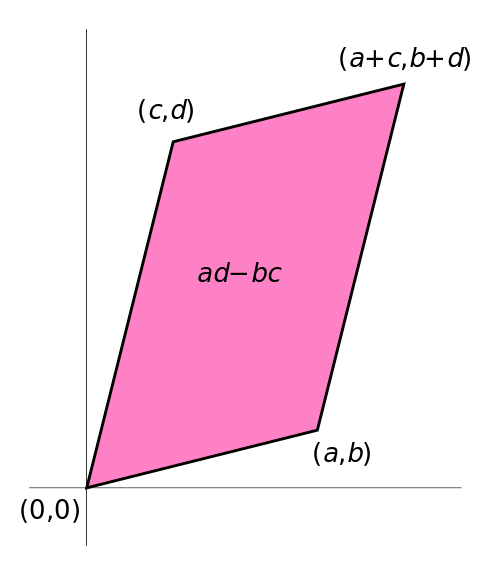
\includegraphics[width=6.94in]{External_Images/determinant} \end{center}

\subsection{Inverse}\label{inverse}

In regular algebra, we are often interested in solving equations such as
\[ 5x=15 \] for \(x\). To do so, we multiply each side of the equation
by the inverse of 5, which is \(1/5\).

\begin{eqnarray*}
5x & = & 15\\
\frac{1}{5}\cdot5\cdot x & = & \frac{1}{5}\cdot15\\
1\cdot x & = & 3\\
x & = & 3
\end{eqnarray*}

For scalars, we know that the inverse of scalar \(a\) is the value that
when multiplied by \(a\) is 1. That is we see to find \(a^{-1}\) such
that \(aa^{-1}=1\).

In the matrix case, I am interested in finding \(\boldsymbol{A}^{-1}\)
such that \(\boldsymbol{A}^{-1}\boldsymbol{A}=\boldsymbol{I}\) and
\(\boldsymbol{A}\boldsymbol{A}^{-1}=\boldsymbol{I}\). For both of these
multiplications to be defined, \(\boldsymbol{A}\) must be a square
matrix and so the inverse is only defined for square matrices.

For a \(2\times2\) matrix \[
\boldsymbol{W}=\left[\begin{array}{cc}
a & b\\
c & d
\end{array}\right]
\] the inverse is given by: \[
\boldsymbol{W}^{-1}=\frac{1}{\det\boldsymbol{W}}\;\left[\begin{array}{cc}
d & -b\\
-c & a
\end{array}\right]
\]

For example, suppose \[
\boldsymbol{W}=\left[\begin{array}{cc}
1 & 2\\
5 & 3
\end{array}\right]
\] then \(\det W=3-10=-7\) and

\begin{eqnarray*}
\boldsymbol{W}^{-1} & = & \frac{1}{-7}\;\left[\begin{array}{cc}
3 & -2\\
-5 & 1
\end{array}\right]\\
 & = & \left[\begin{array}{cc}
-\frac{3}{7} & \frac{2}{7}\\
\frac{5}{7} & -\frac{1}{7}
\end{array}\right]
\end{eqnarray*}

and thus

\begin{eqnarray*}
\boldsymbol{W}\boldsymbol{W}^{-1} & = & \left[\begin{array}{cc}
1 & 2\\
5 & 3
\end{array}\right]\left[\begin{array}{cc}
-\frac{3}{7} & \frac{2}{7}\\
\frac{5}{7} & -\frac{1}{7}
\end{array}\right]\\
\\
 & = & \left[\begin{array}{cc}
-\frac{3}{7}+\frac{10}{7}\;\;\; & \frac{2}{7}-\frac{2}{7}\\
\\
-\frac{15}{7}+\frac{15}{7}\;\;\; & \frac{10}{7}-\frac{3}{7}
\end{array}\right]\\
\\
 & = & \left[\begin{array}{cc}
1 & 0\\
0 & 1
\end{array}\right]=\boldsymbol{I}_{2}
\end{eqnarray*}

Not every square matrix has an inverse. If the determinant of the matrix
(which we think of as some measure of the magnitude or \emph{size} of
the matrix) is zero, then the formula would require us to divide by
zero. Just as we cannot find the inverse of zero (i.e.~solve \(0x=1\)
for \(x\)), a matrix with zero determinate is said to have no inverse.

\section{Exercises}\label{exercises}

Consider the following matrices: \[
\mathbf{A}=\left[\begin{array}{ccc}
1 & 2 & 3\\
6 & 5 & 4
\end{array}\right]\;\;\;\;\;\;\;\mathbf{B}=\left[\begin{array}{ccc}
6 & 4 & 3\\
8 & 7 & 6
\end{array}\right]\;\;\;\;\;\;\;\mathbf{c}=\left[\begin{array}{c}
1\\
2\\
3
\end{array}\right]\;\;\;\;\;\;\;\mathbf{d}=\left[\begin{array}{c}
4\\
5\\
6
\end{array}\right]\;\;\;\;\;\;\;\mathbf{E}=\left[\begin{array}{cc}
1 & 2\\
2 & 6
\end{array}\right]
\]

\begin{enumerate}
\def\labelenumi{\arabic{enumi}.}
\tightlist
\item
  Find \(\mathbf{Bc}\)
\item
  Find \(\mathbf{AB}^{T}\)
\item
  Find \(\mathbf{c}^{T}\mathbf{d}\)
\item
  Find \(\mathbf{cd}^{T}\)
\item
  Confirm that
  \(\mathbf{E}^{-1}=\left[\begin{array}{cc}  3 & -1\\  -1 & 1/2 \end{array}\right]\)
  is the inverse of \(\mathbf{E}\) by calculating
  \(\mathbf{E}\mathbf{E}^{-1}=\mathbf{I}\).
\end{enumerate}

\chapter{Parameter Estimation}\label{parameter-estimation}

We have previously looked at ANOVA and regression models and, in many
ways, they felt very similar. In this chapter we will introduce the
theory that allows us to understand both models as a particular flavor
of a larger class of models known as \emph{linear models}.

First we clarify what a linear model is. A linear model is a model where
the data (which we will denote using roman letters as \(\boldsymbol{x}\)
and \(\boldsymbol{y}\)) and parameters of interest (which we denote
using Greek letters such as \(\boldsymbol{\alpha}\) and
\(\boldsymbol{\beta}\)) interact only via addition and multiplication.
The following are linear models:

\begin{longtable}[]{@{}ll@{}}
\toprule
\begin{minipage}[b]{0.25\columnwidth}\raggedright\strut
Model\strut
\end{minipage} & \begin{minipage}[b]{0.60\columnwidth}\raggedright\strut
Formula\strut
\end{minipage}\tabularnewline
\midrule
\endhead
\begin{minipage}[t]{0.25\columnwidth}\raggedright\strut
ANOVA\strut
\end{minipage} & \begin{minipage}[t]{0.60\columnwidth}\raggedright\strut
\(y_{ij}=\mu+\tau_{i}+\epsilon_{ij}\)\strut
\end{minipage}\tabularnewline
\begin{minipage}[t]{0.25\columnwidth}\raggedright\strut
Simple Regression\strut
\end{minipage} & \begin{minipage}[t]{0.60\columnwidth}\raggedright\strut
\(y_{i}=\beta_{0}+\beta_{1}x_{i}+\epsilon_{i}\)\strut
\end{minipage}\tabularnewline
\begin{minipage}[t]{0.25\columnwidth}\raggedright\strut
Quadratic Term\strut
\end{minipage} & \begin{minipage}[t]{0.60\columnwidth}\raggedright\strut
\(y_{i}=\beta_{0}+\beta_{1}x_{i}+\beta_{2}x_{i}^{2}+\epsilon_{i}\)\strut
\end{minipage}\tabularnewline
\begin{minipage}[t]{0.25\columnwidth}\raggedright\strut
General Regression\strut
\end{minipage} & \begin{minipage}[t]{0.60\columnwidth}\raggedright\strut
\(y_{i}=\beta_{0}+\beta_{1}x_{i,1}+\beta_{2}x_{i,2}+\dots+\beta_{p}x_{i,p}+\epsilon_{i}\)\strut
\end{minipage}\tabularnewline
\bottomrule
\end{longtable}

Notice in the Quadratic model, the square is not a parameter and we can
consider \(x_{i}^{2}\) as just another column of data. This leads to the
second example of multiple regression where we just add more slopes for
other covariates where the \(p\)th covariate is denoted
\(\boldsymbol{x}_{\cdot,p}\) and might be some transformation (such as
\(x^{2}\) or \(\log x\)) of another column of data. The critical point
is that the transformation to the data \(\boldsymbol{x}\) does not
depend on a parameter. Thus the following is \emph{not} a linear model
\[
y_{i}=\beta_{0}+\beta_{1}x_{i}^{\alpha}+\epsilon_{i}
\]

\section{Simple Regression}\label{simple-regression}

We would like to represent all linear models in a similar compact matrix
representation. This will allow us to make the transition between simple
and multiple regression (and ANCOVA) painlessly.

To begin, we think about how to write the simple regression model using
matrices and vectors that correspond the the data and the parameters.
Notice we have

\[\begin{aligned}
y_{1} & =  \beta_{0}+\beta_{1}x_{1}+\epsilon_{1}\\
y_{2} & =  \beta_{0}+\beta_{1}x_{2}+\epsilon_{2}\\
y_{3} & =  \beta_{0}+\beta_{1}x_{3}+\epsilon_{3}\\
 & \vdots\\
y_{n-1} & =  \beta_{0}+\beta_{1}x_{n-1}+\epsilon_{n-1}\\
y_{n} & =  \beta_{0}+\beta_{1}x_{n}+\epsilon_{n}
\end{aligned}\]

where, as usual,
\(\epsilon_{i}\stackrel{iid}{\sim}N\left(0,\sigma^{2}\right)\). These
equations can be written using matrices as RR \[
\underset{\boldsymbol{y}}{\underbrace{\left[\begin{array}{c}
y_{1}\\
y_{2}\\
y_{3}\\
\vdots\\
y_{n-1}\\
y_{n}
\end{array}\right]}}=\underset{\boldsymbol{X}}{\underbrace{\left[\begin{array}{cc}
1 & x_{1}\\
1 & x_{2}\\
1 & x_{3}\\
\vdots & \vdots\\
1 & x_{n-1}\\
1 & x_{n}
\end{array}\right]}}\underset{\boldsymbol{\beta}}{\underbrace{\left[\begin{array}{c}
\beta_{0}\\
\beta_{1}
\end{array}\right]}}+\underset{\boldsymbol{\epsilon}}{\underbrace{\left[\begin{array}{c}
\epsilon_{1}\\
\epsilon_{2}\\
\epsilon_{3}\\
\vdots\\
\epsilon_{n-1}\\
\epsilon_{n}
\end{array}\right]}}
\]

and we compactly write the model as

\[
\boldsymbol{y}=\boldsymbol{X}\boldsymbol{\beta}+\boldsymbol{\epsilon}
\] where \(\boldsymbol{X}\) is referred to as the \emph{design matrix}
and \(\boldsymbol{\beta}\) is the vector of \emph{location parameters}
we are interested in estimating.

\subsection{Estimation of Location
Paramters}\label{estimation-of-location-paramters}

Our next goal is to find the best estimate of \(\boldsymbol{\beta}\)
given the data. To justify the formula, consider the case where there is
no error terms (i.e. \(\epsilon_{i}=0\) for all \(i\)). Thus we have \[
\boldsymbol{y}=\boldsymbol{X}\boldsymbol{\beta}
\] and our goal is to solve for \(\boldsymbol{\beta}\). To do this, we
must use a matrix inverse, but since inverses only exist for square
matrices, we pre-multiple by \(\boldsymbol{X}^{T}\) (notice that
\(\boldsymbol{X}^{T}\boldsymbol{X}\) is a symmetric \(2\times2\)
matrix). \[
\boldsymbol{X}^{T}\boldsymbol{y}=\boldsymbol{X}^{T}\boldsymbol{X}\boldsymbol{\beta}
\] and then pre-multiply by
\(\left(\boldsymbol{X}^{T}\boldsymbol{X}\right)^{-1}\).

\[\begin{eqnarray*}
\left(\boldsymbol{X}^{T}\boldsymbol{X}\right)^{-1}\boldsymbol{X}^{T}\boldsymbol{y} & = & \left(\boldsymbol{X}^{T}\boldsymbol{X}\right)^{-1}\boldsymbol{X}^{T}\boldsymbol{X}\boldsymbol{\beta}\\
\left(\boldsymbol{X}^{T}\boldsymbol{X}\right)^{-1}\boldsymbol{X}^{T}\boldsymbol{y} & = & \boldsymbol{\beta}
\end{eqnarray*}\]

This exercise suggests that
\(\left(\boldsymbol{X}^{T}\boldsymbol{X}\right)^{-1}\boldsymbol{X}^{T}\boldsymbol{y}\)
is a good place to start when looking for the maximum-likelihood
estimator for \(\boldsymbol{\beta}\). It turns out that this quantity is
in fact the maximum-likelihood estimator (and equivalently minimizes the
sum-of-squared error). Therefore we will use it as our estimate of
\(\boldsymbol{\beta}\). \[
\hat{\boldsymbol{\beta}}=\left(\boldsymbol{X}^{T}\boldsymbol{X}\right)^{-1}\boldsymbol{X}^{T}\boldsymbol{y}
\]

\subsection{Estimation of Variance
Parameter}\label{estimation-of-variance-parameter}

Recall our model is \[
y_{i}=\beta_{0}+\beta_{1}x_{i}+\epsilon_{i}
\] where \(\epsilon_{i}\stackrel{iid}{\sim}N\left(0,\sigma^{2}\right)\).

Using our estimates \(\hat{\boldsymbol{\beta}}\) we can obtain predicted
values for the regression line at any x-value. In particular we can find
the predicted value for each \(x_i\) value in our dataset. \[
\hat{y}_i = \hat{\beta}_0 + \hat{\beta}_1 x_i
\] Using matrix notation, I would write
\(\hat{\boldsymbol{y}}=\boldsymbol{X}\hat{\boldsymbol{\beta}}\).

As usual we will find estimates of the noise terms (which we will call
residuals or errors) via \[\begin{eqnarray*}
\hat{\epsilon}_{i} & = & y_{i}-\hat{y}_{i}\\
 & = & y_{i}-\left(\hat{\beta}_{0}+\hat{\beta}_{1}x_{i}\right)
\end{eqnarray*}\]

Writing \(\hat{\boldsymbol{y}}\) in matrix terms we have
\[\begin{eqnarray*}
\hat{\boldsymbol{y}} & = & \boldsymbol{X}\hat{\boldsymbol{\beta}}\\
 & = & \boldsymbol{X}\left(\boldsymbol{X}^{T}\boldsymbol{X}\right)^{-1}\boldsymbol{X}^{T}\boldsymbol{y}\\
 & = & \boldsymbol{H}\boldsymbol{y}
\end{eqnarray*}\] where
\(\boldsymbol{H}=\boldsymbol{X}\left(\boldsymbol{X}^{T}\boldsymbol{X}\right)^{-1}\boldsymbol{X}^{T}\)
is often called the \emph{hat-matrix} because it takes \(y\) to
\(\hat{y}\) and has many interesting theoretical
properties.\footnote{Mathematically, $\boldsymbol{H}$ is the projection matrix that takes
a vector in $n$-dimensional space and projects it onto a $p$-dimension
subspace spanned by the vectors in $\boldsymbol{X}$. Projection matrices
have many useful properties and much of the theory of linear models
utilizes $\boldsymbol{H}$. }

We can now estimate the error terms via

\[\begin{eqnarray*}
\hat{\boldsymbol{\epsilon}} & = & \boldsymbol{y}-\hat{\boldsymbol{y}}\\
 & = & \boldsymbol{y}-\boldsymbol{H}\boldsymbol{y}\\
 & = & \left(\boldsymbol{I}_{n}-\boldsymbol{H}\right)\boldsymbol{y}
\end{eqnarray*}\]

As usual we estimate \(\sigma^{2}\) using the mean-squared error
\[\begin{eqnarray*}
\hat{\sigma}^{2} & = & \frac{1}{n-2}\;\sum_{i=1}^{n}\hat{\epsilon}_{i}^{2}\\
\\
 & = & \frac{1}{n-2}\;\hat{\boldsymbol{\epsilon}}^{T}\hat{\boldsymbol{\epsilon}}
\end{eqnarray*}\]

In the general linear model case where \(\boldsymbol{\beta}\) has \(p\)
elements (and thus we have \(n-p\) degrees of freedom), the formula is
\[\begin{eqnarray*}
\hat{\sigma}^{2} & = & \frac{1}{n-p}\;\hat{\boldsymbol{\epsilon}}^{T}\hat{\boldsymbol{\epsilon}}
\end{eqnarray*}\]

\subsection{Expectation and variance of a random
vector}\label{expectation-and-variance-of-a-random-vector}

Just as we needed to derive the expected value and variance of
\(\bar{x}\) in the previous semester, we must now do the same for
\(\hat{\boldsymbol{\beta}}\). But to do this, we need some properties of
expectations and variances.

In the following, let \(\boldsymbol{A}_{n\times p}\) and
\(\boldsymbol{b}_{n\times1}\) be constants and
\(\boldsymbol{\epsilon}_{n\times1}\) be a random vector.

Expectations are very similar to the scalar case where \[
E\left[\boldsymbol{\epsilon}\right]=\left[\begin{array}{c}
E\left[\epsilon_{1}\right]\\
E\left[\epsilon_{2}\right]\\
\vdots\\
E\left[\epsilon_{n}\right]
\end{array}\right]
\] and any constants are pulled through the expectation \[
E\left[\boldsymbol{A}^{T}\boldsymbol{\epsilon}+\boldsymbol{b}\right]=\boldsymbol{A}^{T}\,E\left[\boldsymbol{\epsilon}\right]+\boldsymbol{b}
\]

Variances are a little different. The variance of the vector
\(\boldsymbol{\epsilon}\) is \[
Var\left(\boldsymbol{\epsilon}\right)=\left[\begin{array}{cccc}
Var\left(\epsilon_{1}\right) & Cov\left(\epsilon_{1},\epsilon_{2}\right) & \dots & Cov\left(\epsilon_{1},\epsilon_{n}\right)\\
Cov\left(\epsilon_{2},\epsilon_{1}\right) & Var\left(\epsilon_{2}\right) & \dots & Cov\left(\epsilon_{2},\epsilon_{n}\right)\\
\vdots & \vdots & \ddots & \vdots\\
Cov\left(\epsilon_{n},\epsilon_{1}\right) & Cov\left(\epsilon_{n},\epsilon_{2}\right) & \dots & Var\left(\epsilon_{1}\right)
\end{array}\right]
\] and additive constants are ignored, but multiplicative constants are
pulled out as follows: \[
Var\left(\boldsymbol{A}^{T}\boldsymbol{\epsilon}+\boldsymbol{b}\right)=Var\left(\boldsymbol{A}^{T}\boldsymbol{\epsilon}\right)=\boldsymbol{A}^{T}\,Var\left(\boldsymbol{\epsilon}\right)\,\boldsymbol{A}
\]

\subsection{Variance of Location
Parameters}\label{variance-of-location-parameters}

We next derive the sampling variance of our estimator
\(\hat{\boldsymbol{\beta}}\) by first noting that \(\boldsymbol{X}\) and
\(\boldsymbol{\beta}\) are constants and therefore

\begin{eqnarray*}
Var\left(\boldsymbol{y}\right) & = & Var\left(\boldsymbol{X}\boldsymbol{\beta}+\boldsymbol{\epsilon}\right)\\
 & = & Var\left(\boldsymbol{\epsilon}\right)\\
 & = & \sigma^{2}\boldsymbol{I}_{n}
\end{eqnarray*}

because the error terms are independent and therefore
\(Cov\left(\epsilon_{i},\epsilon_{j}\right)=0\) when \(i\ne j\) and
\(Var\left(\epsilon_{i}\right)=\sigma^{2}\). Recalling that constants
come out of the variance operator as the constant \emph{squared,
}

\begin{eqnarray*}
Var\left(\hat{\boldsymbol{\beta}}\right) & = & Var\left(\left(\boldsymbol{X}^{T}\boldsymbol{X}\right)^{-1}\boldsymbol{X}^{T}\boldsymbol{y}\right)\\
 & = & \left(\boldsymbol{X}^{T}\boldsymbol{X}\right)^{-1}\boldsymbol{X}^{T}\,Var\left(\boldsymbol{y}\right)\,\boldsymbol{X}\left(\boldsymbol{X}^{T}\boldsymbol{X}\right)^{-1}\\
 & = & \left(\boldsymbol{X}^{T}\boldsymbol{X}\right)^{-1}\boldsymbol{X}^{T}\,\sigma^{2}\boldsymbol{I}_{n}\,\boldsymbol{X}\left(\boldsymbol{X}^{T}\boldsymbol{X}\right)^{-1}\\
 & = & \sigma^{2}\left(\boldsymbol{X}^{T}\boldsymbol{X}\right)^{-1}\boldsymbol{X}^{T}\boldsymbol{X}\left(\boldsymbol{X}^{T}\boldsymbol{X}\right)^{-1}\\
 & = & \sigma^{2}\left(\boldsymbol{X}^{T}\boldsymbol{X}\right)^{-1}
\end{eqnarray*}

Using this, the standard error (i.e.~the estimated standard deviation)
of \(\hat{\beta}_{j}\) (for any \(j\) in \(1,\dots,p\)) is \[
StdErr\left(\hat{\beta}_{j}\right)=\sqrt{\hat{\sigma}^{2}\left[\left(\boldsymbol{X}^{T}\boldsymbol{X}\right)^{-1}\right]_{jj}}
\]

\subsection{Confidence intervals and hypothesis
tests}\label{confidence-intervals-and-hypothesis-tests}

We can now state the general method of creating confidence intervals and
perform hypothesis tests for any element of \(\boldsymbol{\beta}\).

The confidence interval formula is (as usual) \[
\hat{\beta}_{j}\pm t_{n-p}^{1-\alpha/2}\,StdErr\left(\hat{\beta}_{j}\right)
\] and a test statistic for testing \(H_{0}:\,\beta_{j}=0\) versus
\(H_{a}:\,\beta_{j}\ne0\) is \[
t_{n-p}=\frac{\hat{\beta}_{j}-0}{StdErr\left(\hat{\beta}_{j}\right)}
\]

\subsection{Summary of pertinent
results}\label{summary-of-pertinent-results}

\begin{itemize}
\item
  \(\hat{\boldsymbol{\beta}}=\left(\boldsymbol{X}^{T}\boldsymbol{X}\right)^{-1}\boldsymbol{X}^{T}\boldsymbol{y}\)
  is the unbiased maximum-likelihood estimator of
  \(\boldsymbol{\beta}\).
\item
  The Central Limit Theorem applies to each element of
  \(\boldsymbol{\beta}\). That is, as \(n\to\infty\), the distribution
  of
  \(\hat{\beta}_{j}\to N\left(\beta_{j},\left[\sigma^{2}\left(\boldsymbol{X}^{T}\boldsymbol{X}\right)^{-1}\right]_{jj}\right)\).
\item
  The error terms can be calculated via

  \begin{eqnarray*}
  \hat{\boldsymbol{y}} & = & \boldsymbol{X}\hat{\boldsymbol{\beta}}\\
  \hat{\boldsymbol{\epsilon}} & = & \boldsymbol{y}-\hat{\boldsymbol{y}}
  \end{eqnarray*}
\item
  The estimate of \(\sigma^{2}\) is \[
  \hat{\sigma}^{2}=\frac{1}{n-p}\;\hat{\boldsymbol{\epsilon}}^{T}\hat{\boldsymbol{\epsilon}}
  \]
\item
  The standard error (i.e.~the estimated standard deviation) of
  \(\hat{\beta}_{j}\) (for any \(j\) in \(1,\dots,p\)) is \[
  StdErr\left(\hat{\beta}_{j}\right)=\sqrt{\hat{\sigma}^{2}\left[\left(\boldsymbol{X}^{T}\boldsymbol{X}\right)^{-1}\right]_{jj}}
  \]
\end{itemize}

\subsection{An example in R}\label{an-example-in-r}

Here we will work an example in R and see the calculations. Consider the
following data:

\begin{Shaded}
\begin{Highlighting}[]
\KeywordTok{library}\NormalTok{(ggplot2)}
\NormalTok{n <-}\StringTok{ }\DecValTok{20}
\NormalTok{x <-}\StringTok{ }\KeywordTok{seq}\NormalTok{(}\DecValTok{0}\NormalTok{,}\DecValTok{10}\NormalTok{, }\DataTypeTok{length=}\NormalTok{n)}
\NormalTok{y <-}\StringTok{ }\NormalTok{-}\DecValTok{3} \NormalTok{+}\StringTok{ }\DecValTok{2}\NormalTok{*x +}\StringTok{ }\KeywordTok{rnorm}\NormalTok{(n, }\DataTypeTok{sd=}\DecValTok{2}\NormalTok{)}
\NormalTok{my.data <-}\StringTok{ }\KeywordTok{data.frame}\NormalTok{(}\DataTypeTok{x=}\NormalTok{x, }\DataTypeTok{y=}\NormalTok{y)}
\KeywordTok{ggplot}\NormalTok{(my.data) +}\StringTok{ }\KeywordTok{geom_point}\NormalTok{(}\KeywordTok{aes}\NormalTok{(}\DataTypeTok{x=}\NormalTok{x,}\DataTypeTok{y=}\NormalTok{y))}
\end{Highlighting}
\end{Shaded}

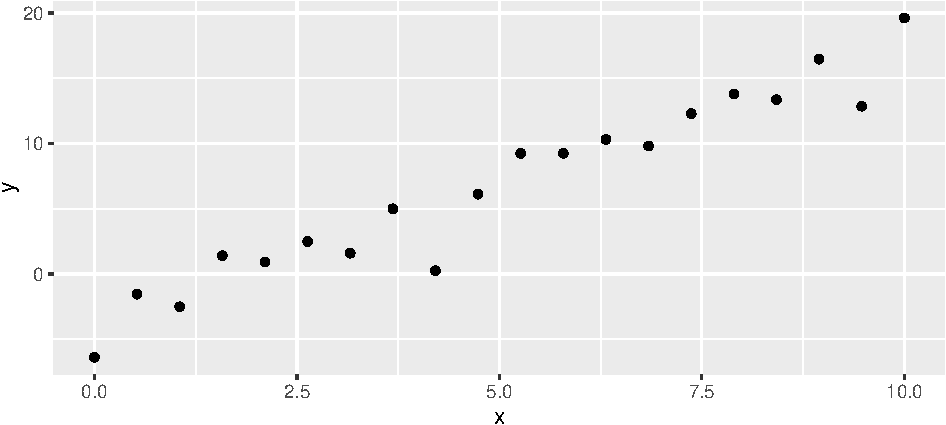
\includegraphics{Statistical_Methods_II_files/figure-latex/unnamed-chunk-3-1.pdf}

First we must create the design matrix \(\boldsymbol{X}\). Recall \[
\boldsymbol{X}=\left[\begin{array}{cc}
1 & x_{1}\\
1 & x_{2}\\
1 & x_{3}\\
\vdots & \vdots\\
1 & x_{n-1}\\
1 & x_{n}
\end{array}\right]
\] and can be created in R via the following:

\begin{Shaded}
\begin{Highlighting}[]
\NormalTok{X <-}\StringTok{ }\KeywordTok{cbind}\NormalTok{( }\KeywordTok{rep}\NormalTok{(}\DecValTok{1}\NormalTok{,n), x)}
\end{Highlighting}
\end{Shaded}

Given \(\boldsymbol{X}\) and \(\boldsymbol{y}\) we can calculate \[
\hat{\boldsymbol{\beta}}=\left(\boldsymbol{X}^{T}\boldsymbol{X}\right)^{-1}\boldsymbol{X}^{T}\boldsymbol{y}
\] in R using the following code:

\begin{Shaded}
\begin{Highlighting}[]
\NormalTok{XtXinv <-}\StringTok{ }\KeywordTok{solve}\NormalTok{( }\KeywordTok{t}\NormalTok{(X) %*%}\StringTok{ }\NormalTok{X )}
\NormalTok{beta.hat <-}\StringTok{ }\NormalTok{XtXinv %*%}\StringTok{ }\KeywordTok{t}\NormalTok{(X) %*%}\StringTok{ }\NormalTok{y}
\NormalTok{beta.hat}
\end{Highlighting}
\end{Shaded}

\begin{verbatim}
##        [,1]
##   -2.845342
## x  2.038477
\end{verbatim}

Our next step is to calculate the predicted values
\(\hat{\boldsymbol{y}}\) and the residuals
\(\hat{\boldsymbol{\epsilon}}\)

\begin{eqnarray*}
\hat{\boldsymbol{y}} & = & \boldsymbol{X}\hat{\boldsymbol{\beta}}\\
\hat{\boldsymbol{\epsilon}} & = & \boldsymbol{y}-\hat{\boldsymbol{y}}
\end{eqnarray*}

\begin{Shaded}
\begin{Highlighting}[]
\NormalTok{y.hat <-}\StringTok{ }\NormalTok{X %*%}\StringTok{ }\NormalTok{beta.hat}
\NormalTok{residuals <-}\StringTok{ }\NormalTok{y -}\StringTok{ }\NormalTok{y.hat}
\end{Highlighting}
\end{Shaded}

Now that we have the residuals, we can calculate \(\hat{\sigma}^{2}\)
and the standard errors of \(\hat{\beta}_{j}\) \[
\hat{\sigma}^{2}=\frac{1}{n-p}\,\hat{\boldsymbol{\epsilon}}^{T}\hat{\boldsymbol{\epsilon}}
\] \[
StdErr\left(\hat{\beta}_{j}\right)=\sqrt{\hat{\sigma}^{2}\left[\left(\boldsymbol{X}^{T}\boldsymbol{X}\right)^{-1}\right]_{jj}}
\]

\begin{Shaded}
\begin{Highlighting}[]
\NormalTok{sigma2.hat <-}\StringTok{ }\NormalTok{( }\KeywordTok{t}\NormalTok{(residuals) %*%}\StringTok{ }\NormalTok{residuals) /}\StringTok{ }\NormalTok{(n}\DecValTok{-2}\NormalTok{)}
\NormalTok{sigma.hat <-}\StringTok{ }\KeywordTok{sqrt}\NormalTok{( sigma2.hat )}
\NormalTok{std.errs <-}\StringTok{ }\KeywordTok{sqrt}\NormalTok{( sigma2.hat *}\StringTok{ }\KeywordTok{diag}\NormalTok{(XtXinv) )}
\end{Highlighting}
\end{Shaded}

We now print out the important values and compare them to the summary
output given by the \texttt{lm()} function in R.

\begin{Shaded}
\begin{Highlighting}[]
\NormalTok{beta.hat}
\end{Highlighting}
\end{Shaded}

\begin{verbatim}
##        [,1]
##   -2.845342
## x  2.038477
\end{verbatim}

\begin{Shaded}
\begin{Highlighting}[]
\NormalTok{sigma.hat}
\end{Highlighting}
\end{Shaded}

\begin{verbatim}
##          [,1]
## [1,] 1.690702
\end{verbatim}

\begin{Shaded}
\begin{Highlighting}[]
\NormalTok{std.errs}
\end{Highlighting}
\end{Shaded}

\begin{verbatim}
## [1] 0.7286009 0.1245690
\end{verbatim}

\begin{Shaded}
\begin{Highlighting}[]
\NormalTok{model <-}\StringTok{ }\KeywordTok{lm}\NormalTok{(y~x)}
\KeywordTok{summary}\NormalTok{(model)}
\end{Highlighting}
\end{Shaded}

\begin{verbatim}
## 
## Call:
## lm(formula = y ~ x)
## 
## Residuals:
##     Min      1Q  Median      3Q     Max 
## -3.0465 -1.3949  0.5699  1.1023  2.9904 
## 
## Coefficients:
##             Estimate Std. Error t value Pr(>|t|)    
## (Intercept)  -2.8453     0.7286  -3.905  0.00104 ** 
## x             2.0385     0.1246  16.364 2.98e-12 ***
## ---
## Signif. codes:  0 '***' 0.001 '**' 0.01 '*' 0.05 '.' 0.1 ' ' 1
## 
## Residual standard error: 1.691 on 18 degrees of freedom
## Multiple R-squared:  0.937,  Adjusted R-squared:  0.9335 
## F-statistic: 267.8 on 1 and 18 DF,  p-value: 2.979e-12
\end{verbatim}

We calculate \(95\%\) confidence intervals via:

\begin{Shaded}
\begin{Highlighting}[]
\NormalTok{lwr <-}\StringTok{ }\NormalTok{beta.hat -}\StringTok{ }\KeywordTok{qt}\NormalTok{(.}\DecValTok{975}\NormalTok{, n}\DecValTok{-2}\NormalTok{) *}\StringTok{ }\NormalTok{std.errs}
\NormalTok{upr <-}\StringTok{ }\NormalTok{beta.hat +}\StringTok{ }\KeywordTok{qt}\NormalTok{(.}\DecValTok{975}\NormalTok{, n}\DecValTok{-2}\NormalTok{) *}\StringTok{ }\NormalTok{std.errs}
\NormalTok{CI <-}\StringTok{ }\KeywordTok{cbind}\NormalTok{(lwr,upr)}
\KeywordTok{colnames}\NormalTok{(CI) <-}\StringTok{ }\KeywordTok{c}\NormalTok{(}\StringTok{'lower'}\NormalTok{,}\StringTok{'upper'}\NormalTok{)}
\KeywordTok{rownames}\NormalTok{(CI) <-}\StringTok{ }\KeywordTok{c}\NormalTok{(}\StringTok{'Intercept'}\NormalTok{, }\StringTok{'x'}\NormalTok{)}
\NormalTok{CI}
\end{Highlighting}
\end{Shaded}

\begin{verbatim}
##               lower     upper
## Intercept -4.376076 -1.314608
## x          1.776767  2.300187
\end{verbatim}

These intervals are the same as what we get when we use the
\texttt{confint()} function.

\begin{Shaded}
\begin{Highlighting}[]
\KeywordTok{confint}\NormalTok{(model)}
\end{Highlighting}
\end{Shaded}

\begin{verbatim}
##                 2.5 %    97.5 %
## (Intercept) -4.376076 -1.314608
## x            1.776767  2.300187
\end{verbatim}

\section{ANOVA model}\label{anova-model}

The anova model is also a linear model and all we must do is create a
appropriate design matrix. Given the design matrix \(\boldsymbol{X}\),
all the calculations are identical as in the simple regression case.

\subsection{Cell means representation}\label{cell-means-representation}

Recall the cell means representation is \[
y_{i,j}=\mu_{i}+\epsilon_{i,j}
\] where \(y_{i,j}\) is the \(j\)th observation within the \(i\)th
group. To clearly show the creation of the \(\boldsymbol{X}\) matrix,
let the number of groups be \(p=3\) and the number of observations per
group be \(n_{i}=4\). We now expand the formula to show all the data.

\begin{eqnarray*}
y_{1,1} & = & \mu_{1}+\epsilon_{1,1}\\
y_{1,2} & = & \mu_{1}+\epsilon_{1,2}\\
y_{1,3} & = & \mu_{1}+\epsilon_{1,3}\\
y_{1,4} & = & \mu_{1}+\epsilon_{1,4}\\
y_{2,1} & = & \mu_{2}+\epsilon_{2,1}\\
y_{2,2} & = & \mu_{2}+\epsilon_{2,2}\\
y_{2,3} & = & \mu_{2}+\epsilon_{2,3}\\
y_{2,4} & = & \mu_{2}+\epsilon_{2,4}\\
y_{3,1} & = & \mu_{3}+\epsilon_{3,1}\\
y_{3,2} & = & \mu_{3}+\epsilon_{3,2}\\
y_{3,3} & = & \mu_{3}+\epsilon_{3,3}\\
y_{3,4} & = & \mu_{3}+\epsilon_{3,4}
\end{eqnarray*}

In an effort to write the model as
\(\boldsymbol{y}=\boldsymbol{X}\boldsymbol{\beta}+\boldsymbol{\epsilon}\)
we will write the above as

\begin{eqnarray*}
y_{1,1} & = & 1\mu_{1}+0\mu_{2}+0\mu_{3}+\epsilon_{1,1}\\
y_{1,2} & = & 1\mu_{1}+0\mu_{2}+0\mu_{3}+\epsilon_{1,2}\\
y_{1,3} & = & 1\mu_{1}+0\mu_{2}+0\mu_{3}+\epsilon_{1,3}\\
y_{1,4} & = & 1\mu_{1}+0\mu_{2}+0\mu_{3}+\epsilon_{1,4}\\
y_{2,1} & = & 0\mu+1\mu_{2}+0\mu_{3}+\epsilon_{2,1}\\
y_{2,2} & = & 0\mu+1\mu_{2}+0\mu_{3}+\epsilon_{2,2}\\
y_{2,3} & = & 0\mu+1\mu_{2}+0\mu_{3}+\epsilon_{2,3}\\
y_{2,4} & = & 0\mu+1\mu_{2}+0\mu_{3}+\epsilon_{2,4}\\
y_{3,1} & = & 0\mu+0\mu_{2}+1\mu_{3}+\epsilon_{3,1}\\
y_{3,2} & = & 0\mu+0\mu_{2}+1\mu_{3}+\epsilon_{3,2}\\
y_{3,3} & = & 0\mu+0\mu_{2}+1\mu_{3}+\epsilon_{3,3}\\
y_{3,4} & = & 0\mu+0\mu_{2}+1\mu_{3}+\epsilon_{3,4}
\end{eqnarray*}

and we will finally be able to write the matrix version \[
\underset{\boldsymbol{y}}{\underbrace{\left[\begin{array}{c}
y_{1,1}\\
y_{1,2}\\
y_{1,3}\\
y_{1,4}\\
y_{2,1}\\
y_{2,2}\\
y_{2,3}\\
y_{2,4}\\
y_{3,1}\\
y_{3,2}\\
y_{3,3}\\
y_{3,4}
\end{array}\right]}}=\underset{\mathbf{X}}{\underbrace{\left[\begin{array}{ccc}
1 & 0 & 0\\
1 & 0 & 0\\
1 & 0 & 0\\
1 & 0 & 0\\
0 & 1 & 0\\
0 & 1 & 0\\
0 & 1 & 0\\
0 & 1 & 0\\
0 & 0 & 1\\
0 & 0 & 1\\
0 & 0 & 1\\
0 & 0 & 1
\end{array}\right]}}\underset{\boldsymbol{\beta}}{\underbrace{\left[\begin{array}{c}
\mu_{1}\\
\mu_{2}\\
\mu_{3}
\end{array}\right]}}+\underset{\boldsymbol{\epsilon}}{\underbrace{\left[\begin{array}{c}
\epsilon_{1,1}\\
\epsilon_{1,2}\\
\epsilon_{1,3}\\
\epsilon_{1,4}\\
\epsilon_{2,1}\\
\epsilon_{2,2}\\
\epsilon_{2,3}\\
\epsilon_{2,4}\\
\epsilon_{3,1}\\
\epsilon_{3,2}\\
\epsilon_{3,3}\\
\epsilon_{3,4}
\end{array}\right]}}
\] \[
\] Notice that each column of the \(\boldsymbol{X}\) matrix is acting as
an indicator if the observation is an element of the appropriate group.
As such, these are often called \emph{indicator variables}. Another term
for these, which I find less helpful, is \emph{dummy variables}.

\subsection{Offset from reference
group}\label{offset-from-reference-group}

In this model representation of ANOVA, we have an overall mean and then
offsets from the control group (which will be group one). The model is
thus \[
y_{i,j}=\mu+\tau_{i}+\epsilon_{i,j}
\] where \(\tau_{1}=0\). We can write this in matrix form as \[
\underset{\boldsymbol{y}}{\underbrace{\left[\begin{array}{c}
y_{1,1}\\
y_{1,2}\\
y_{1,3}\\
y_{1,4}\\
y_{2,1}\\
y_{2,2}\\
y_{2,3}\\
y_{2,4}\\
y_{3,1}\\
y_{3,2}\\
y_{3,3}\\
y_{3,4}
\end{array}\right]}}=\underset{\mathbf{X}}{\underbrace{\left[\begin{array}{ccc}
1 & 0 & 0\\
1 & 0 & 0\\
1 & 0 & 0\\
1 & 0 & 0\\
1 & 1 & 0\\
1 & 1 & 0\\
1 & 1 & 0\\
1 & 1 & 0\\
1 & 0 & 1\\
1 & 0 & 1\\
1 & 0 & 1\\
1 & 0 & 1
\end{array}\right]}}\underset{\boldsymbol{\beta}}{\underbrace{\left[\begin{array}{c}
\mu\\
\tau_{2}\\
\tau_{3}
\end{array}\right]}}+\underset{\boldsymbol{\epsilon}}{\underbrace{\left[\begin{array}{c}
\epsilon_{1,1}\\
\epsilon_{1,2}\\
\epsilon_{1,3}\\
\epsilon_{1,4}\\
\epsilon_{2,1}\\
\epsilon_{2,2}\\
\epsilon_{2,3}\\
\epsilon_{2,4}\\
\epsilon_{3,1}\\
\epsilon_{3,2}\\
\epsilon_{3,3}\\
\epsilon_{3,4}
\end{array}\right]}}
\]

\section{Exercises}\label{exercises-1}

\begin{enumerate}
\def\labelenumi{\arabic{enumi}.}
\item
  We will do a simple ANOVA analysis on example 8.2 from Ott \&
  Longnecker using the matrix representation of the model. A clinical
  psychologist wished to compare three methods for reducing hostility
  levels in university students, and used a certain test (HLT) to
  measure the degree of hostility. A high score on the test indicated
  great hostility. The psychologist used 24 students who obtained high
  and nearly equal scores in the experiment. eight were selected at
  random from among the 24 problem cases and were treated with method 1.
  Seven of the remaining 16 students were selected at random and treated
  with method 2. The remaining nine students were treated with method 3.
  All treatments were continued for a one-semester period. Each student
  was given the HLT test at the end of the semester, with the results
  show in the following table. (This analysis was done in section 8.3 of
  my STA 570 notes)

  \begin{longtable}[]{@{}ll@{}}
  \toprule
  Method & Values\tabularnewline
  \midrule
  \endhead
  1 & 96, 79, 91, 85, 83, 91, 82, 87\tabularnewline
  2 & 77, 76, 74, 73, 78, 71, 80\tabularnewline
  3 & 66, 73, 69, 66, 77, 73, 71, 70, 74\tabularnewline
  \bottomrule
  \end{longtable}

  We will be using the cell means model of ANOVA
  \[ y_{ij}=\beta_{i}+\epsilon_{ij} \] where \(\beta_{i}\) is the mean
  of group \(i\) and
  \(\epsilon_{ij}\stackrel{iid}{\sim}N\left(0,\sigma^{2}\right)\).

  \begin{enumerate}
  \def\labelenumii{\alph{enumii}.}
  \item
    Create one vector of all 24 hostility test scores \texttt{y}. (Use
    the \texttt{c()} function.)
  \item
    Create a design matrix \texttt{X} with dummy variables for columns
    that code for what group an observation belongs to. Notice that
    \texttt{X} will be a \(24\) rows by \(3\) column matrix. \emph{Hint:
    An R function that might be handy is \texttt{cbind(a,b)} which will
    bind two vectors or matrices together along the columns. (There is
    also a corresponding \texttt{rbind()} function that binds
    vectors/matrices along rows.) Also you'll like to have the repeat
    command \texttt{rep()}.}
  \end{enumerate}

  \begin{enumerate}
  \def\labelenumii{\alph{enumii})}
  \setcounter{enumii}{2}
  \item
    Find \(\hat{\boldsymbol{\beta}}\) using the matrix formula given in
    class. \emph{Hint: The R function \texttt{t(A)} computes the matrix
    transpose \(\mathbf{A}^{T}\), \texttt{solve(A)} computes
    \(\mathbf{A}^{-1}\), and the operator \texttt{\%*\%} does matrix
    multiplication (used as \texttt{A\ \%*\%\ B}).}
  \item
    Examine the matrix
    \(\left(\mathbf{X}^{T}\mathbf{X}\right)^{-1}\mathbf{X}^{T}\). What
    do you notice about it? In particular, think about the result when
    you right multiply by \(\mathbf{y}\). How does this matrix calculate
    the appropriate group means and using the appropriate group sizes
    \(n_i\)?
  \end{enumerate}
\item
  We will calculate the y-intercept and slope estimates in a simple
  linear model using matrix notation. We will use a data set that gives
  the diameter at breast height (DBH) versus tree height for a randomly
  selected set of trees. In addition, for each tree, a ground
  measurement of crown closure (CC) was taken. Larger values of crown
  closure indicate more shading and is often associated with taller tree
  morphology (possibly). We will be interested in creating a regression
  model that predicts height based on DBH and CC. In the interest of
  reduced copying, we will only use 10 observations. \emph{(Note: I made
  this data up and the DBH values might be unrealistic. Don't make fun
  of me.)}

  \begin{longtable}[]{@{}cllllllllll@{}}
  \toprule
  \begin{minipage}[t]{0.13\columnwidth}\centering\strut
  \textbf{DBH}\strut
  \end{minipage} &
  \begin{minipage}[t]{0.05\columnwidth}\raggedright\strut
  30.5\strut
  \end{minipage} &
  \begin{minipage}[t]{0.05\columnwidth}\raggedright\strut
  31.5\strut
  \end{minipage} &
  \begin{minipage}[t]{0.05\columnwidth}\raggedright\strut
  31.7\strut
  \end{minipage} &
  \begin{minipage}[t]{0.05\columnwidth}\raggedright\strut
  32.3\strut
  \end{minipage} &
  \begin{minipage}[t]{0.05\columnwidth}\raggedright\strut
  33.3\strut
  \end{minipage} &
  \begin{minipage}[t]{0.04\columnwidth}\raggedright\strut
  35\strut
  \end{minipage} &
  \begin{minipage}[t]{0.05\columnwidth}\raggedright\strut
  35.4\strut
  \end{minipage} &
  \begin{minipage}[t]{0.05\columnwidth}\raggedright\strut
  35.6\strut
  \end{minipage} &
  \begin{minipage}[t]{0.05\columnwidth}\raggedright\strut
  36.3\strut
  \end{minipage} &
  \begin{minipage}[t]{0.05\columnwidth}\raggedright\strut
  37.8\strut
  \end{minipage}\tabularnewline
  \begin{minipage}[t]{0.13\columnwidth}\centering\strut
  \textbf{CC}\strut
  \end{minipage} &
  \begin{minipage}[t]{0.05\columnwidth}\raggedright\strut
  0.74\strut
  \end{minipage} &
  \begin{minipage}[t]{0.05\columnwidth}\raggedright\strut
  0.69\strut
  \end{minipage} &
  \begin{minipage}[t]{0.05\columnwidth}\raggedright\strut
  0.65\strut
  \end{minipage} &
  \begin{minipage}[t]{0.05\columnwidth}\raggedright\strut
  0.72\strut
  \end{minipage} &
  \begin{minipage}[t]{0.05\columnwidth}\raggedright\strut
  0.58\strut
  \end{minipage} &
  \begin{minipage}[t]{0.04\columnwidth}\raggedright\strut
  0.5\strut
  \end{minipage} &
  \begin{minipage}[t]{0.05\columnwidth}\raggedright\strut
  0.6\strut
  \end{minipage} &
  \begin{minipage}[t]{0.05\columnwidth}\raggedright\strut
  0.7\strut
  \end{minipage} &
  \begin{minipage}[t]{0.05\columnwidth}\raggedright\strut
  0.52\strut
  \end{minipage} &
  \begin{minipage}[t]{0.05\columnwidth}\raggedright\strut
  0.6\strut
  \end{minipage}\tabularnewline
  \begin{minipage}[t]{0.13\columnwidth}\centering\strut
  \textbf{Height}\strut
  \end{minipage} &
  \begin{minipage}[t]{0.05\columnwidth}\raggedright\strut
  58\strut
  \end{minipage} &
  \begin{minipage}[t]{0.05\columnwidth}\raggedright\strut
  64\strut
  \end{minipage} &
  \begin{minipage}[t]{0.05\columnwidth}\raggedright\strut
  65\strut
  \end{minipage} &
  \begin{minipage}[t]{0.05\columnwidth}\raggedright\strut
  70\strut
  \end{minipage} &
  \begin{minipage}[t]{0.05\columnwidth}\raggedright\strut
  68\strut
  \end{minipage} &
  \begin{minipage}[t]{0.04\columnwidth}\raggedright\strut
  63\strut
  \end{minipage} &
  \begin{minipage}[t]{0.05\columnwidth}\raggedright\strut
  78\strut
  \end{minipage} &
  \begin{minipage}[t]{0.05\columnwidth}\raggedright\strut
  80\strut
  \end{minipage} &
  \begin{minipage}[t]{0.05\columnwidth}\raggedright\strut
  74\strut
  \end{minipage} &
  \begin{minipage}[t]{0.05\columnwidth}\raggedright\strut
  76\strut
  \end{minipage}\tabularnewline
  \bottomrule
  \end{longtable}

  We are interested in fitting the regression model
  \[y_{i}=\beta_{0}+\beta_{1}x_{i,1}+\beta_{2}x_{i,2}+\epsilon_{i}\]
  where \(\beta_{0}\) is the y-intercept and \(\beta_{1}\) is the slope
  parameter associated with DBH and \(\beta_{2}\) is the slope parameter
  associated with Crown Closure.

  \begin{enumerate}
  \def\labelenumii{\alph{enumii})}
  \tightlist
  \item
    Create a vector of all 10 heights \(\mathbf{y}\).
  \item
    Create the design matrix \(\mathbf{X}\).
  \item
    Find \(\hat{\boldsymbol{\beta}}\) using the matrix formula given in
    class.
  \item
    Compare your results to the estimated coefficients you get using the
    \texttt{lm()} function. To add the second predictor to the model,
    your call to \texttt{lm()} should look something like
    \texttt{lm(Height\ \textasciitilde{}\ DBH\ +\ CrownClosure)}.
  \end{enumerate}
\end{enumerate}

\chapter{Inference}\label{inference}

\section{F-tests}\label{f-tests}

We wish to develop a rigorous way to compare nested models and decide if
a complicated model explains enough more variability than a simple model
to justify the additional intellectual effort of thinking about the data
in the complicated fashion.

It is important to specify that we are developing a way of testing
nested models. By nested, we mean that the simple model can be created
from the full model just by setting one or more model parameters to
zero.

\subsection{Theory}\label{theory}

Recall that in the simple regression and ANOVA cases we were interested
in comparing a simple model versus a more complex model. For each model
we computed the residual sum of squares (RSS) and said that if the
complicated model performed much better than the simple then
\(RSS_{simple}\gg RSS_{complex}\). To do this we needed to standardize
by the number of parameters added to the model and the degrees of
freedom remaining in the full model. We first defined
\(RSS_{diff}=RSS_{simple}-RSS_{complex}\) and let \(df_{diff}\) be the
number of parameters difference between the simple and complex models.
Then we had
\[F=\frac{RSS_{difference}/df_{diff}}{RSS_{complex}/df_{complex}}\] and
we claimed that if the null hypothesis was true (i.e.~the complex model
is an unnecessary obfuscation of the simple), then this ratio follows an
F -distribution with degrees of freedom \(df_{diff}\) and
\(df_{complex}\).

The critical assumption for the F-test to be appropriate is that the
error terms are independent and normally distributed with constant
variance.

We will consider a data set from Johnson and Raven (1973) which also
appears in Weisberg (1985). This data set is concerned with the number
of tortoise species on \(n=30\) different islands in the Galapagos. The
variables of interest in the data set are:

\begin{longtable}[]{@{}ll@{}}
\toprule
Variable & Description\tabularnewline
\midrule
\endhead
\texttt{Species} & Number of tortoise species found on the
island\tabularnewline
\texttt{Endimics} & Number of tortoise species endemic to the
island\tabularnewline
\texttt{Elevation} & Elevation of the highest point on the
island\tabularnewline
\texttt{Area} & Area of the island (km\(^2\))\tabularnewline
\texttt{Nearest} & Distance to the nearest neighboring island
(km)\tabularnewline
\texttt{Scruz} & Distance to the Santa Cruz islands (km)\tabularnewline
\texttt{Adjacent} & Area of the nearest adjacent island
(km\(^2\))\tabularnewline
\bottomrule
\end{longtable}

We will first read in the data set from the package \texttt{faraway}.

\begin{Shaded}
\begin{Highlighting}[]
\KeywordTok{library}\NormalTok{(faraway)    }\CommentTok{# load the library }
\KeywordTok{data}\NormalTok{(gala)          }\CommentTok{# import the data set}
\KeywordTok{head}\NormalTok{(gala)          }\CommentTok{# show the first couple of rows}
\end{Highlighting}
\end{Shaded}

\begin{verbatim}
##              Species Endemics  Area Elevation Nearest Scruz Adjacent
## Baltra            58       23 25.09       346     0.6   0.6     1.84
## Bartolome         31       21  1.24       109     0.6  26.3   572.33
## Caldwell           3        3  0.21       114     2.8  58.7     0.78
## Champion          25        9  0.10        46     1.9  47.4     0.18
## Coamano            2        1  0.05        77     1.9   1.9   903.82
## Daphne.Major      18       11  0.34       119     8.0   8.0     1.84
\end{verbatim}

First we will create the full model that predicts the number of species
as a function of elevation, area, nearest, scruz and adjacent. Notice
that this model has \(p=6\) \(\beta_{i}\) values (one for each
coefficient plus the intercept).

\[ y_i = \beta_0 + \beta_1 Area_i + \beta_2 Elevation_i + \beta_3 Nearest_i + \beta_4 Scruz_i + \beta_5 Adjacent_i + \epsilon_i\]

We can happily fit this model just by adding terms on the left hand side
of the model formula. Notice that R creates the design matrix \(X\) for
us.

\begin{Shaded}
\begin{Highlighting}[]
\NormalTok{M.c <-}\StringTok{ }\KeywordTok{lm}\NormalTok{(Species ~}\StringTok{ }\NormalTok{Area +}\StringTok{ }\NormalTok{Elevation +}\StringTok{ }\NormalTok{Nearest +}\StringTok{ }\NormalTok{Scruz +}\StringTok{ }\NormalTok{Adjacent, }\DataTypeTok{data=}\NormalTok{gala)}
\KeywordTok{model.matrix}\NormalTok{(M.c)  }\CommentTok{# this is the design matrix X.}
\end{Highlighting}
\end{Shaded}

\begin{verbatim}
##              (Intercept)    Area Elevation Nearest Scruz Adjacent
## Baltra                 1   25.09       346     0.6   0.6     1.84
## Bartolome              1    1.24       109     0.6  26.3   572.33
## Caldwell               1    0.21       114     2.8  58.7     0.78
## Champion               1    0.10        46     1.9  47.4     0.18
## Coamano                1    0.05        77     1.9   1.9   903.82
## Daphne.Major           1    0.34       119     8.0   8.0     1.84
## Daphne.Minor           1    0.08        93     6.0  12.0     0.34
## Darwin                 1    2.33       168    34.1 290.2     2.85
## Eden                   1    0.03        71     0.4   0.4    17.95
## Enderby                1    0.18       112     2.6  50.2     0.10
## Espanola               1   58.27       198     1.1  88.3     0.57
## Fernandina             1  634.49      1494     4.3  95.3  4669.32
## Gardner1               1    0.57        49     1.1  93.1    58.27
## Gardner2               1    0.78       227     4.6  62.2     0.21
## Genovesa               1   17.35        76    47.4  92.2   129.49
## Isabela                1 4669.32      1707     0.7  28.1   634.49
## Marchena               1  129.49       343    29.1  85.9    59.56
## Onslow                 1    0.01        25     3.3  45.9     0.10
## Pinta                  1   59.56       777    29.1 119.6   129.49
## Pinzon                 1   17.95       458    10.7  10.7     0.03
## Las.Plazas             1    0.23        94     0.5   0.6    25.09
## Rabida                 1    4.89       367     4.4  24.4   572.33
## SanCristobal           1  551.62       716    45.2  66.6     0.57
## SanSalvador            1  572.33       906     0.2  19.8     4.89
## SantaCruz              1  903.82       864     0.6   0.0     0.52
## SantaFe                1   24.08       259    16.5  16.5     0.52
## SantaMaria             1  170.92       640     2.6  49.2     0.10
## Seymour                1    1.84       147     0.6   9.6    25.09
## Tortuga                1    1.24       186     6.8  50.9    17.95
## Wolf                   1    2.85       253    34.1 254.7     2.33
## attr(,"assign")
## [1] 0 1 2 3 4 5
\end{verbatim}

All the usual calculations from chapter two can be calculated and we can
see the summary table for this regression as follows:

\begin{Shaded}
\begin{Highlighting}[]
\KeywordTok{summary}\NormalTok{(M.c)}
\end{Highlighting}
\end{Shaded}

\begin{verbatim}
## 
## Call:
## lm(formula = Species ~ Area + Elevation + Nearest + Scruz + Adjacent, 
##     data = gala)
## 
## Residuals:
##      Min       1Q   Median       3Q      Max 
## -111.679  -34.898   -7.862   33.460  182.584 
## 
## Coefficients:
##              Estimate Std. Error t value Pr(>|t|)    
## (Intercept)  7.068221  19.154198   0.369 0.715351    
## Area        -0.023938   0.022422  -1.068 0.296318    
## Elevation    0.319465   0.053663   5.953 3.82e-06 ***
## Nearest      0.009144   1.054136   0.009 0.993151    
## Scruz       -0.240524   0.215402  -1.117 0.275208    
## Adjacent    -0.074805   0.017700  -4.226 0.000297 ***
## ---
## Signif. codes:  0 '***' 0.001 '**' 0.01 '*' 0.05 '.' 0.1 ' ' 1
## 
## Residual standard error: 60.98 on 24 degrees of freedom
## Multiple R-squared:  0.7658, Adjusted R-squared:  0.7171 
## F-statistic:  15.7 on 5 and 24 DF,  p-value: 6.838e-07
\end{verbatim}

\subsection{Testing All Covariates}\label{testing-all-covariates}

The first test we might want to do is to test if any of the covariates
are significant. That is to say that we want to test the full model
versus the simple null hypothesis model \[y_{i}=\beta_{0}+\epsilon_{i}\]
that has no covariates and only a y-intercept. So we will create a
simple model

\begin{Shaded}
\begin{Highlighting}[]
\NormalTok{M.s <-}\StringTok{ }\KeywordTok{lm}\NormalTok{(Species ~}\StringTok{ }\DecValTok{1}\NormalTok{, }\DataTypeTok{data=}\NormalTok{gala)}
\end{Highlighting}
\end{Shaded}

and calculate the appropriate Residual Sums of Squares (RSS) for each
model, along with the difference in degrees of freedom between the two
models.

\begin{Shaded}
\begin{Highlighting}[]
\NormalTok{RSS.c <-}\StringTok{ }\KeywordTok{sum}\NormalTok{(}\KeywordTok{resid}\NormalTok{(M.c)^}\DecValTok{2}\NormalTok{)}
\NormalTok{RSS.s <-}\StringTok{ }\KeywordTok{sum}\NormalTok{(}\KeywordTok{resid}\NormalTok{(M.s)^}\DecValTok{2}\NormalTok{)}
\NormalTok{df.diff <-}\StringTok{ }\DecValTok{5}               \CommentTok{# complex model has 5 additional parameters}
\NormalTok{df.c <-}\StringTok{ }\DecValTok{30} \NormalTok{-}\StringTok{ }\DecValTok{6}             \CommentTok{# complex model has 24 degrees of freedom left}
\end{Highlighting}
\end{Shaded}

The F-statistic for this test is therefore

\begin{Shaded}
\begin{Highlighting}[]
\NormalTok{F.stat <-}\StringTok{  }\NormalTok{( (RSS.s -}\StringTok{ }\NormalTok{RSS.c) /}\StringTok{ }\NormalTok{df.diff ) /}\StringTok{ }\NormalTok{( RSS.c /}\StringTok{ }\NormalTok{df.c )}
\NormalTok{F.stat}
\end{Highlighting}
\end{Shaded}

\begin{verbatim}
## [1] 15.69941
\end{verbatim}

and should be compared against the F-distribution with \(5\) and \(24\)
degrees of freedom. Because a large difference between RSS.s and RSS.c
would be evidence for the alternative, larger model, the p-value for
this test is \[p-value=P\left(F_{5,24}\ge\mathtt{F.stat}\right)\]

\begin{Shaded}
\begin{Highlighting}[]
\NormalTok{p.value <-}\StringTok{  }\DecValTok{1} \NormalTok{-}\StringTok{ }\KeywordTok{pf}\NormalTok{(}\FloatTok{15.699}\NormalTok{, }\DecValTok{5}\NormalTok{, }\DecValTok{24}\NormalTok{)}
\NormalTok{p.value}
\end{Highlighting}
\end{Shaded}

\begin{verbatim}
## [1] 6.839486e-07
\end{verbatim}

Both the F.stat and its p-value are given at the bottom of the summary
table. However, I might be interested in creating an ANOVA table for
this situation.

\begin{longtable}[]{@{}llllll@{}}
\toprule
Source & df & Sum Sq & Mean Sq & F & p-value\tabularnewline
\midrule
\endhead
Difference & \(p-1\) & \(RSS_d\) & \(MSE_d = RSS_d / (p-1)\) &
\(MSE_d/MSE_c\) & \(P(F > F_{p-1,n-p})\)\tabularnewline
Complex & \(n-p\) & \(RSS_c\) & \(MSE_c = RSS_c / (n-p)\) &
&\tabularnewline
Simple & \(n-1\) & \(RSS_s\) & & &\tabularnewline
\bottomrule
\end{longtable}

This table can be obtained from R by using the \texttt{anova()} function
on the two models of interest. As usual with R, it does not show the
simple row, but rather concentrates on the difference row.

\begin{Shaded}
\begin{Highlighting}[]
\KeywordTok{anova}\NormalTok{(M.s, M.c)}
\end{Highlighting}
\end{Shaded}

\begin{verbatim}
## Analysis of Variance Table
## 
## Model 1: Species ~ 1
## Model 2: Species ~ Area + Elevation + Nearest + Scruz + Adjacent
##   Res.Df    RSS Df Sum of Sq      F    Pr(>F)    
## 1     29 381081                                  
## 2     24  89231  5    291850 15.699 6.838e-07 ***
## ---
## Signif. codes:  0 '***' 0.001 '**' 0.01 '*' 0.05 '.' 0.1 ' ' 1
\end{verbatim}

\subsection{Testing a Single
Covariate}\label{testing-a-single-covariate}

For a particular covariate, \(\beta_{j}\), we might wish to perform a
test to see if it can be removed from the model. It can be shown that
the F-statistic can be re-written as

\[\begin{aligned}
F   &=  \frac{\left[RSS_{s}-RSS_{c}\right]/1}{RSS_{c}/\left(n-p\right)}\\
    &=  \vdots\\
    &=  \left[\frac{\hat{\beta_{j}}}{SE\left(\hat{\beta}_{j}\right)}\right]^{2}\\
    &= t^{2}
\end{aligned}\] where \(t\) has a t-distribution with \(n-p\) degrees of
freedom under the null hypothesis that the simple model is sufficient.

We consider the case of removing the covariate \texttt{Area} from the
model and will calculate our test statistic using both methods.

\begin{Shaded}
\begin{Highlighting}[]
\NormalTok{M.c <-}\StringTok{ }\KeywordTok{lm}\NormalTok{(Species ~}\StringTok{ }\NormalTok{Area +}\StringTok{ }\NormalTok{Elevation +}\StringTok{ }\NormalTok{Nearest +}\StringTok{ }\NormalTok{Scruz +}\StringTok{ }\NormalTok{Adjacent, }\DataTypeTok{data=}\NormalTok{gala)}
\NormalTok{M.s <-}\StringTok{ }\KeywordTok{lm}\NormalTok{(Species ~}\StringTok{        }\NormalTok{Elevation +}\StringTok{ }\NormalTok{Nearest +}\StringTok{ }\NormalTok{Scruz +}\StringTok{ }\NormalTok{Adjacent, }\DataTypeTok{data=}\NormalTok{gala)}
\NormalTok{RSS.c <-}\StringTok{ }\KeywordTok{sum}\NormalTok{( }\KeywordTok{resid}\NormalTok{(M.c)^}\DecValTok{2} \NormalTok{)}
\NormalTok{RSS.s <-}\StringTok{ }\KeywordTok{sum}\NormalTok{( }\KeywordTok{resid}\NormalTok{(M.s)^}\DecValTok{2} \NormalTok{)}
\NormalTok{df.d <-}\StringTok{ }\DecValTok{1}
\NormalTok{df.c <-}\StringTok{ }\DecValTok{30-6}
\NormalTok{F.stat <-}\StringTok{ }\NormalTok{((RSS.s -}\StringTok{ }\NormalTok{RSS.c)/}\DecValTok{1}\NormalTok{) /}\StringTok{ }\NormalTok{(RSS.c /}\StringTok{ }\NormalTok{df.c)}
\NormalTok{F.stat}
\end{Highlighting}
\end{Shaded}

\begin{verbatim}
## [1] 1.139792
\end{verbatim}

\begin{Shaded}
\begin{Highlighting}[]
\DecValTok{1} \NormalTok{-}\StringTok{ }\KeywordTok{pf}\NormalTok{(F.stat, }\DecValTok{1}\NormalTok{, }\DecValTok{24}\NormalTok{)}
\end{Highlighting}
\end{Shaded}

\begin{verbatim}
## [1] 0.296318
\end{verbatim}

\begin{Shaded}
\begin{Highlighting}[]
\KeywordTok{sqrt}\NormalTok{(F.stat)}
\end{Highlighting}
\end{Shaded}

\begin{verbatim}
## [1] 1.067611
\end{verbatim}

To calculate it using the estimated coefficient and its standard error,
we must grab those values from the summary table

\begin{Shaded}
\begin{Highlighting}[]
\NormalTok{temp <-}\StringTok{ }\KeywordTok{summary}\NormalTok{(M.c)}
\NormalTok{temp$coefficients}
\end{Highlighting}
\end{Shaded}

\begin{verbatim}
##                 Estimate  Std. Error      t value     Pr(>|t|)
## (Intercept)  7.068220709 19.15419782  0.369016796 7.153508e-01
## Area        -0.023938338  0.02242235 -1.067610554 2.963180e-01
## Elevation    0.319464761  0.05366280  5.953187968 3.823409e-06
## Nearest      0.009143961  1.05413595  0.008674366 9.931506e-01
## Scruz       -0.240524230  0.21540225 -1.116628222 2.752082e-01
## Adjacent    -0.074804832  0.01770019 -4.226216850 2.970655e-04
\end{verbatim}

\begin{Shaded}
\begin{Highlighting}[]
\NormalTok{beta.area <-}\StringTok{ }\NormalTok{temp$coefficients[}\DecValTok{2}\NormalTok{,}\DecValTok{1}\NormalTok{]}
\NormalTok{SE.beta.area <-}\StringTok{ }\NormalTok{temp$coefficients[}\DecValTok{2}\NormalTok{,}\DecValTok{2}\NormalTok{]}
\NormalTok{t <-}\StringTok{ }\NormalTok{beta.area /}\StringTok{ }\NormalTok{SE.beta.area}
\NormalTok{t}
\end{Highlighting}
\end{Shaded}

\begin{verbatim}
## [1] -1.067611
\end{verbatim}

\begin{Shaded}
\begin{Highlighting}[]
\DecValTok{2} \NormalTok{*}\StringTok{ }\KeywordTok{pt}\NormalTok{(t, }\DecValTok{24}\NormalTok{)}
\end{Highlighting}
\end{Shaded}

\begin{verbatim}
## [1] 0.296318
\end{verbatim}

All that hand calculation is tedious, so we can again use the anova()
command to compare the two models.

\begin{Shaded}
\begin{Highlighting}[]
\KeywordTok{anova}\NormalTok{(M.s, M.c)}
\end{Highlighting}
\end{Shaded}

\begin{verbatim}
## Analysis of Variance Table
## 
## Model 1: Species ~ Elevation + Nearest + Scruz + Adjacent
## Model 2: Species ~ Area + Elevation + Nearest + Scruz + Adjacent
##   Res.Df   RSS Df Sum of Sq      F Pr(>F)
## 1     25 93469                           
## 2     24 89231  1    4237.7 1.1398 0.2963
\end{verbatim}

\subsection{Testing a Subset of
Covariates}\label{testing-a-subset-of-covariates}

Often a researcher will want to remove a subset of covariates from the
model. In the Galapagos example, Area, Nearest, and Scruz all have
non-significant p-values and would be removed when comparing the full
model to the model without that one covariate. While each of them might
be non-significant, is the sum of all three significant?

Because the individual \(\hat{\beta}_{j}\) values are not independent,
then we cannot claim that the subset is not statistically significant
just because each variable in turn was insignificant. Instead we again
create simple and complex models in the same fashion as we have
previously done.

\begin{Shaded}
\begin{Highlighting}[]
\NormalTok{M.c <-}\StringTok{ }\KeywordTok{lm}\NormalTok{(Species ~}\StringTok{ }\NormalTok{Area +}\StringTok{ }\NormalTok{Elevation +}\StringTok{ }\NormalTok{Nearest +}\StringTok{ }\NormalTok{Scruz +}\StringTok{ }\NormalTok{Adjacent, }\DataTypeTok{data=}\NormalTok{gala)}
\NormalTok{M.s <-}\StringTok{ }\KeywordTok{lm}\NormalTok{(Species ~}\StringTok{        }\NormalTok{Elevation +}\StringTok{                   }\NormalTok{Adjacent, }\DataTypeTok{data=}\NormalTok{gala)}
\KeywordTok{anova}\NormalTok{(M.s, M.c)}
\end{Highlighting}
\end{Shaded}

\begin{verbatim}
## Analysis of Variance Table
## 
## Model 1: Species ~ Elevation + Adjacent
## Model 2: Species ~ Area + Elevation + Nearest + Scruz + Adjacent
##   Res.Df    RSS Df Sum of Sq      F Pr(>F)
## 1     27 100003                           
## 2     24  89231  3     10772 0.9657  0.425
\end{verbatim}

We find a large p-value associated with this test and can safely stay
with the null hypothesis, that the simple model is sufficient to explain
the observed variability in the number of species of tortoise.

\section{Confidence Intervals for location
parameters}\label{confidence-intervals-for-location-parameters}

Recall that
\[\hat{\boldsymbol{\beta}}\sim N\left(\boldsymbol{\beta},\,\sigma^{2}\left(\mathbf{X}^{T}\mathbf{X}\right)^{-1}\right)\]
and it is easy to calculate the estimate of \(\sigma^{2}\). This
estimate will be the ``average'' squared residual
\[\hat{\sigma}^{2}=\frac{RSS}{df}\] where \(RSS\) is the residual sum of
squares and \(df\) is the degrees of freedom \(n-p\) where \(p\) is the
number of \(\beta_{j}\) parameters. Therefore the standard error of the
\(\hat{\beta}_{j}\) values is
\[SE\left(\hat{\beta}_{j}\right)=\sqrt{\hat{\sigma}^{2}\left(\mathbf{X}^{T}\mathbf{X}\right)_{jj}^{-1}}\]

We can see this calculation in the summary regression table. We again
consider the Galapagos Island data set. First we must create the design
matrix

\begin{Shaded}
\begin{Highlighting}[]
\NormalTok{y <-}\StringTok{ }\NormalTok{gala$Species}
\NormalTok{X <-}\StringTok{ }\KeywordTok{cbind}\NormalTok{( }\KeywordTok{rep}\NormalTok{(}\DecValTok{1}\NormalTok{,}\DecValTok{30}\NormalTok{), gala$Elevation, gala$Adjacent )}
\end{Highlighting}
\end{Shaded}

And then create \(\left(\mathbf{X}^{T}\mathbf{X}\right)^{-1}\)

\begin{Shaded}
\begin{Highlighting}[]
\NormalTok{XtXinv <-}\StringTok{ }\KeywordTok{solve}\NormalTok{(  }\KeywordTok{t}\NormalTok{(X) %*%}\StringTok{ }\NormalTok{X )}
\NormalTok{XtXinv}
\end{Highlighting}
\end{Shaded}

\begin{verbatim}
##               [,1]          [,2]          [,3]
## [1,]  6.094829e-02 -8.164025e-05  9.312123e-06
## [2,] -8.164025e-05  2.723835e-07 -7.126027e-08
## [3,]  9.312123e-06 -7.126027e-08  6.478031e-08
\end{verbatim}

\begin{Shaded}
\begin{Highlighting}[]
\KeywordTok{diag}\NormalTok{(XtXinv)}
\end{Highlighting}
\end{Shaded}

\begin{verbatim}
## [1] 6.094829e-02 2.723835e-07 6.478031e-08
\end{verbatim}

Eventually we will need \(\hat{\boldsymbol{\beta}}\)

\begin{Shaded}
\begin{Highlighting}[]
\NormalTok{beta.hat <-}\StringTok{ }\NormalTok{XtXinv %*%}\StringTok{ }\KeywordTok{t}\NormalTok{(X) %*%}\StringTok{ }\NormalTok{y}
\NormalTok{beta.hat}
\end{Highlighting}
\end{Shaded}

\begin{verbatim}
##            [,1]
## [1,]  1.4328722
## [2,]  0.2765683
## [3,] -0.0688855
\end{verbatim}

And now find the estimate \(\hat{\sigma}\)

\begin{Shaded}
\begin{Highlighting}[]
\NormalTok{H <-}\StringTok{ }\NormalTok{X %*%}\StringTok{ }\NormalTok{XtXinv %*%}\StringTok{ }\KeywordTok{t}\NormalTok{(X)}
\NormalTok{y.hat <-}\StringTok{ }\NormalTok{H %*%}\StringTok{ }\NormalTok{y}
\NormalTok{RSS <-}\StringTok{ }\KeywordTok{sum}\NormalTok{( (y-y.hat)^}\DecValTok{2} \NormalTok{)}
\NormalTok{sigma.hat <-}\StringTok{ }\KeywordTok{sqrt}\NormalTok{(  RSS/(}\DecValTok{30-3}\NormalTok{) )}
\NormalTok{sigma.hat}
\end{Highlighting}
\end{Shaded}

\begin{verbatim}
## [1] 60.85898
\end{verbatim}

The standard errors of \(\hat{\beta}\) is thus

\begin{Shaded}
\begin{Highlighting}[]
\KeywordTok{sqrt}\NormalTok{( sigma.hat^}\DecValTok{2} \NormalTok{*}\StringTok{ }\KeywordTok{diag}\NormalTok{(XtXinv) )}
\end{Highlighting}
\end{Shaded}

\begin{verbatim}
## [1] 15.02468680  0.03176253  0.01548981
\end{verbatim}

We can double check that this is what R calculates in the summary table

\begin{Shaded}
\begin{Highlighting}[]
\NormalTok{model <-}\StringTok{ }\KeywordTok{lm}\NormalTok{(Species ~}\StringTok{ }\NormalTok{Elevation +}\StringTok{ }\NormalTok{Adjacent, }\DataTypeTok{data=}\NormalTok{gala)}
\KeywordTok{summary}\NormalTok{(model)}
\end{Highlighting}
\end{Shaded}

\begin{verbatim}
## 
## Call:
## lm(formula = Species ~ Elevation + Adjacent, data = gala)
## 
## Residuals:
##     Min      1Q  Median      3Q     Max 
## -103.41  -34.33  -11.43   22.57  203.65 
## 
## Coefficients:
##             Estimate Std. Error t value Pr(>|t|)    
## (Intercept)  1.43287   15.02469   0.095 0.924727    
## Elevation    0.27657    0.03176   8.707 2.53e-09 ***
## Adjacent    -0.06889    0.01549  -4.447 0.000134 ***
## ---
## Signif. codes:  0 '***' 0.001 '**' 0.01 '*' 0.05 '.' 0.1 ' ' 1
## 
## Residual standard error: 60.86 on 27 degrees of freedom
## Multiple R-squared:  0.7376, Adjusted R-squared:  0.7181 
## F-statistic: 37.94 on 2 and 27 DF,  p-value: 1.434e-08
\end{verbatim}

It is highly desirable to calculate confidence intervals for the
regression parameters. Recall that the general form of a confidence
interval is
\[Estimate\;\pm Critical\,Value\;\cdot\;StandardError\left(Estimate\right)\]
For any specific \(\beta_{j}\) we will have
\[\hat{\beta}_{j}\pm t_{n-p}^{1-\alpha/2}\,\hat{\sigma}\sqrt{\left(\mathbf{X}^{T}\mathbf{X}\right)_{jj}^{-1}}\]
where
\(\hat{\sigma}^{2}\left(\mathbf{X}^{T}\mathbf{X}\right)_{jj}^{-1}\) is
the \([j,j]\) element of the variance/covariance of
\(\hat{\boldsymbol{\beta}}\).

To demonstrate this, we return to the Galapagos Island data set.

Finally we can calculate confidence intervals for our three
\(\beta_{j}\) values

\begin{Shaded}
\begin{Highlighting}[]
\NormalTok{lower <-}\StringTok{ }\NormalTok{beta.hat -}\StringTok{ }\KeywordTok{qt}\NormalTok{(.}\DecValTok{975}\NormalTok{, }\DecValTok{27}\NormalTok{) *}\StringTok{ }\NormalTok{sigma.hat *}\StringTok{ }\KeywordTok{sqrt}\NormalTok{( }\KeywordTok{diag}\NormalTok{(XtXinv) )}
\NormalTok{upper <-}\StringTok{ }\NormalTok{beta.hat +}\StringTok{ }\KeywordTok{qt}\NormalTok{(.}\DecValTok{975}\NormalTok{, }\DecValTok{27}\NormalTok{) *}\StringTok{ }\NormalTok{sigma.hat *}\StringTok{ }\KeywordTok{sqrt}\NormalTok{( }\KeywordTok{diag}\NormalTok{(XtXinv) )}
\KeywordTok{cbind}\NormalTok{(lower, upper)}
\end{Highlighting}
\end{Shaded}

\begin{verbatim}
##            [,1]        [,2]
## [1,] -29.395239 32.26098305
## [2,]   0.211397  0.34173962
## [3,]  -0.100668 -0.03710303
\end{verbatim}

That is certainly a lot of work to do by hand (even with R doing all the
matrix multiplication) but we can get these from R by using the
confint() command.

\begin{Shaded}
\begin{Highlighting}[]
\KeywordTok{confint}\NormalTok{(model)}
\end{Highlighting}
\end{Shaded}

\begin{verbatim}
##                  2.5 %      97.5 %
## (Intercept) -29.395239 32.26098305
## Elevation     0.211397  0.34173962
## Adjacent     -0.100668 -0.03710303
\end{verbatim}

\section{Prediction and Confidence Intervals for a
response}\label{prediction-and-confidence-intervals-for-a-response}

Given a vector of predictor covariates \(\boldsymbol{x}_{0}\) (think of
\(\boldsymbol{x}_{0}^{T}\) as potentially one row in \(\boldsymbol{X}\).
Because we might want to predict some other values than what we observe,
we do not restrict ourselves to \emph{only} rows in \(\boldsymbol{X}\)),
we want to make inference on the expected value \(\hat{y}_{0}\). We can
calculate the value by
\[\hat{y}_{0}=\boldsymbol{x}_{0}^{T}\hat{\boldsymbol{\beta}}\] and we
are interested in two different types of predictions.

\begin{enumerate}
\def\labelenumi{\arabic{enumi}.}
\item
  We might be interested in the uncertainty of a new data point. This
  uncertainty has two components: the uncertainty of the regression
  model and uncertainty of a new data point from its expected value.
\item
  Second, we might be interested in only the uncertainty about the
  regression model.
\end{enumerate}

We note that because \(\boldsymbol{x}_{0}^{T}\) is just a constant, we
can calculate the variance of this value as \[ \begin{aligned}
Var\left(\boldsymbol{x}_{0}^{T}\hat{\boldsymbol{\beta}}\right)  
  &= \boldsymbol{x}_{0}^{T}\,Var\left(\hat{\boldsymbol{\beta}}\right)\,\boldsymbol{x}_{0} \\
    &=  \boldsymbol{x}_{0}^{T}\,\left(\boldsymbol{X}^{T}\boldsymbol{X}\right)^{-1}\sigma^{2}\,\boldsymbol{x}_{0} \\
    &=  \boldsymbol{x}_{0}^{T}\,\left(\boldsymbol{X}^{T}\boldsymbol{X}\right)^{-1}\,\boldsymbol{x}_{0}\,\sigma^{2}
\end{aligned}\] and use this to calculate two types of intervals. First,
a prediction interval for a new observation is
\[\hat{y}_{0}\pm t_{n-p}^{1-\alpha/2}\,\hat{\sigma}\sqrt{1+\boldsymbol{x}_{0}^{T}\,\left(\boldsymbol{X}^{T}\boldsymbol{X}\right)^{-1}\,\boldsymbol{x}_{0}}\]
and a confidence interval for the mean response for the given
\(\boldsymbol{x}_{0}\) is
\[\hat{y}_{0}\pm t_{n-p}^{1-\alpha/2}\,\hat{\sigma}\sqrt{\boldsymbol{x}_{0}^{T}\,\left(\boldsymbol{X}^{T}\boldsymbol{X}\right)^{-1}\,\boldsymbol{x}_{0}}\]

Again using the Galapagos Island data set as an example, we might be
interested in predicting the number of tortoise species of an island
with highest point \(400\) meters and nearest adjacent island with area
\(200 km^{2}\). We then have
\[\boldsymbol{x}_{0}^{T} = \left[\begin{array}{ccc}1  &  400  &  200\end{array}\right]\]
and we can calculate

\begin{Shaded}
\begin{Highlighting}[]
\NormalTok{x0 <-}\StringTok{ }\KeywordTok{c}\NormalTok{(}\DecValTok{1}\NormalTok{, }\DecValTok{400}\NormalTok{, }\DecValTok{200}\NormalTok{)}
\NormalTok{y0 <-}\StringTok{ }\KeywordTok{t}\NormalTok{(x0) %*%}\StringTok{ }\NormalTok{beta.hat}
\NormalTok{y0}
\end{Highlighting}
\end{Shaded}

\begin{verbatim}
##          [,1]
## [1,] 98.28309
\end{verbatim}

and then calculate
\(\boldsymbol{x}_{0}^{T}\,\left(\boldsymbol{X}^{T}\boldsymbol{X}\right)^{-1}\,\boldsymbol{x}_{0}\)

\begin{Shaded}
\begin{Highlighting}[]
\NormalTok{xt.XtXinv.x <-}\StringTok{ }\KeywordTok{t}\NormalTok{(x0) %*%}\StringTok{ }\KeywordTok{solve}\NormalTok{( }\KeywordTok{t}\NormalTok{(X) %*%}\StringTok{ }\NormalTok{X ) %*%}\StringTok{ }\NormalTok{x0}
\end{Highlighting}
\end{Shaded}

Thus the prediction interval will be

\begin{Shaded}
\begin{Highlighting}[]
\KeywordTok{c}\NormalTok{(y0 -}\StringTok{ }\KeywordTok{qt}\NormalTok{(.}\DecValTok{975}\NormalTok{, }\DecValTok{27}\NormalTok{) *}\StringTok{ }\NormalTok{sigma.hat *}\StringTok{ }\KeywordTok{sqrt}\NormalTok{(}\DecValTok{1} \NormalTok{+}\StringTok{ }\NormalTok{xt.XtXinv.x),}
  \NormalTok{y0 +}\StringTok{ }\KeywordTok{qt}\NormalTok{(.}\DecValTok{975}\NormalTok{, }\DecValTok{27}\NormalTok{) *}\StringTok{ }\NormalTok{sigma.hat *}\StringTok{ }\KeywordTok{sqrt}\NormalTok{(}\DecValTok{1} \NormalTok{+}\StringTok{ }\NormalTok{xt.XtXinv.x))}
\end{Highlighting}
\end{Shaded}

\begin{verbatim}
## [1] -28.70241 225.26858
\end{verbatim}

while a confidence interval for the expectation is

\begin{Shaded}
\begin{Highlighting}[]
\KeywordTok{c}\NormalTok{(y0 -}\StringTok{ }\KeywordTok{qt}\NormalTok{(.}\DecValTok{975}\NormalTok{, }\DecValTok{27}\NormalTok{) *}\StringTok{ }\NormalTok{sigma.hat *}\StringTok{ }\KeywordTok{sqrt}\NormalTok{(xt.XtXinv.x),}
  \NormalTok{y0 +}\StringTok{ }\KeywordTok{qt}\NormalTok{(.}\DecValTok{975}\NormalTok{, }\DecValTok{27}\NormalTok{) *}\StringTok{ }\NormalTok{sigma.hat *}\StringTok{ }\KeywordTok{sqrt}\NormalTok{(xt.XtXinv.x))}
\end{Highlighting}
\end{Shaded}

\begin{verbatim}
## [1]  75.21317 121.35301
\end{verbatim}

These prediction and confidence intervals can be calculated in R using
the predict() function

\begin{Shaded}
\begin{Highlighting}[]
\NormalTok{x0 <-}\StringTok{ }\KeywordTok{data.frame}\NormalTok{(}\DataTypeTok{Elevation=}\DecValTok{400}\NormalTok{, }\DataTypeTok{Adjacent=}\DecValTok{200}\NormalTok{)}
\KeywordTok{predict}\NormalTok{(model, }\DataTypeTok{newdata=}\NormalTok{x0, }\DataTypeTok{interval=}\StringTok{'prediction'}\NormalTok{)}
\end{Highlighting}
\end{Shaded}

\begin{verbatim}
##        fit       lwr      upr
## 1 98.28309 -28.70241 225.2686
\end{verbatim}

\begin{Shaded}
\begin{Highlighting}[]
\KeywordTok{predict}\NormalTok{(model, }\DataTypeTok{newdata=}\NormalTok{x0, }\DataTypeTok{interval=}\StringTok{'confidence'}\NormalTok{)}
\end{Highlighting}
\end{Shaded}

\begin{verbatim}
##        fit      lwr     upr
## 1 98.28309 75.21317 121.353
\end{verbatim}

\section{Interpretation with Correlated
Covariates}\label{interpretation-with-correlated-covariates}

The standard interpretation of the slope parameter is that \(\beta_{j}\)
is the amount of increase in \(y\) for a one unit increase in the
\(j\)th covariate, provided that all other covariates stayed the same.

The difficulty with this interpretation is that covariates are often
related, and the phrase ``all other covariates stayed the same'' is
often not reasonable. For example, if we have a dataset that models the
mean annual temperature of a location as a function of latitude,
longitude, and elevation, then it is not physically possible to hold
latitude, and longitude constant while changing elevation.

One common issue that make interpretation difficult is that covariates
can be highly correlated.

Perch Example: We might be interested in estimating the weight of a fish
based off of its length and width. The dataset we will consider is from
fishes are caught from the same lake (Laengelmavesi) near Tampere in
Finland. The following variables were observed:

\begin{longtable}[]{@{}ll@{}}
\toprule
Variable & Interpretation\tabularnewline
\midrule
\endhead
\texttt{Weight} & Weight (g)\tabularnewline
\texttt{Length.1} & Length from nose to beginning of Tail
(cm)\tabularnewline
\texttt{Length.2} & Length from nose to notch of Tail
(cm)\tabularnewline
\texttt{Length.3} & Length from nose to tip of tail (cm)\tabularnewline
\texttt{Height} & Maximal height as a percentage of
\texttt{Length.3}\tabularnewline
\texttt{Width} & Maximal width as a percentage of
\texttt{Length.3}\tabularnewline
\texttt{Sex} & 0=Female, 1=Male\tabularnewline
\texttt{Species} & Which species of perch (1-7)\tabularnewline
\bottomrule
\end{longtable}

We first look at the data and observe the expected relationship between
length and weight.

\begin{Shaded}
\begin{Highlighting}[]
\NormalTok{file <-}\StringTok{ 'https://raw.githubusercontent.com/dereksonderegger/STA_571_Book/master/data-raw/Fish.csv'}
\NormalTok{fish <-}\StringTok{ }\KeywordTok{read.table}\NormalTok{(file, }\DataTypeTok{header=}\OtherTok{TRUE}\NormalTok{, }\DataTypeTok{skip=}\DecValTok{111}\NormalTok{, }\DataTypeTok{sep=}\StringTok{','}\NormalTok{)}
\KeywordTok{pairs}\NormalTok{(fish[,}\KeywordTok{c}\NormalTok{(}\StringTok{'Weight'}\NormalTok{,}\StringTok{'Length.1'}\NormalTok{,}\StringTok{'Length.2'}\NormalTok{,}\StringTok{'Length.3'}\NormalTok{,}\StringTok{'Height'}\NormalTok{,}\StringTok{'Width'}\NormalTok{)])}
\end{Highlighting}
\end{Shaded}

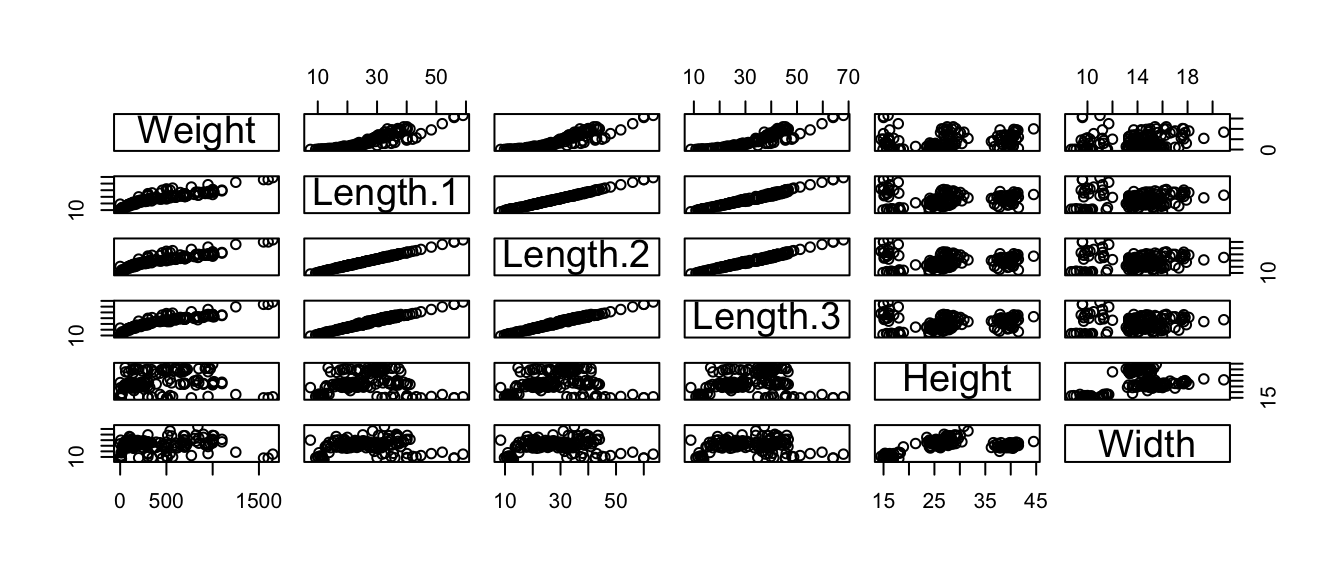
\includegraphics{Statistical_Methods_II_files/figure-latex/unnamed-chunk-39-1.pdf}

Naively, we might consider the linear model with all the length effects
present.

\begin{Shaded}
\begin{Highlighting}[]
\NormalTok{model <-}\StringTok{ }\KeywordTok{lm}\NormalTok{(Weight ~}\StringTok{ }\NormalTok{Length}\FloatTok{.1} \NormalTok{+}\StringTok{ }\NormalTok{Length}\FloatTok{.2} \NormalTok{+}\StringTok{ }\NormalTok{Length}\FloatTok{.3} \NormalTok{+}\StringTok{ }\NormalTok{Height +}\StringTok{ }\NormalTok{Width, }\DataTypeTok{data=}\NormalTok{fish)}
\KeywordTok{summary}\NormalTok{(model)}
\end{Highlighting}
\end{Shaded}

\begin{verbatim}
## 
## Call:
## lm(formula = Weight ~ Length.1 + Length.2 + Length.3 + Height + 
##     Width, data = fish)
## 
## Residuals:
##     Min      1Q  Median      3Q     Max 
## -302.22  -79.72  -39.88   92.63  344.85 
## 
## Coefficients:
##             Estimate Std. Error t value Pr(>|t|)    
## (Intercept) -724.539     77.133  -9.393   <2e-16 ***
## Length.1      32.389     45.134   0.718   0.4741    
## Length.2      -9.184     48.367  -0.190   0.8497    
## Length.3       8.747     16.283   0.537   0.5919    
## Height         4.947      2.768   1.787   0.0759 .  
## Width          8.636      6.972   1.239   0.2174    
## ---
## Signif. codes:  0 '***' 0.001 '**' 0.01 '*' 0.05 '.' 0.1 ' ' 1
## 
## Residual standard error: 132.9 on 152 degrees of freedom
##   (1 observation deleted due to missingness)
## Multiple R-squared:  0.8675, Adjusted R-squared:  0.8631 
## F-statistic:   199 on 5 and 152 DF,  p-value: < 2.2e-16
\end{verbatim}

This is crazy. There is a negative relationship between
\texttt{Length.2} and \texttt{Weight}. That does not make any sense
unless you realize that this is the effect of \texttt{Length.2} assuming
the other covariates are in the model and can be held constant while
changing the value of \texttt{Length.2}, which is obviously ridiculous.

If we remove the highly correlated covariates then we see a much better
behaved model

\begin{Shaded}
\begin{Highlighting}[]
\NormalTok{model <-}\StringTok{ }\KeywordTok{lm}\NormalTok{(Weight ~}\StringTok{ }\NormalTok{Length}\FloatTok{.2} \NormalTok{+}\StringTok{ }\NormalTok{Height +}\StringTok{ }\NormalTok{Width, }\DataTypeTok{data=}\NormalTok{fish)}
\KeywordTok{summary}\NormalTok{(model)}
\end{Highlighting}
\end{Shaded}

\begin{verbatim}
## 
## Call:
## lm(formula = Weight ~ Length.2 + Height + Width, data = fish)
## 
## Residuals:
##     Min      1Q  Median      3Q     Max 
## -306.14  -75.11  -36.45   89.54  337.95 
## 
## Coefficients:
##              Estimate Std. Error t value Pr(>|t|)    
## (Intercept) -701.0750    71.0438  -9.868  < 2e-16 ***
## Length.2      30.4360     0.9841  30.926  < 2e-16 ***
## Height         5.5141     1.4311   3.853 0.000171 ***
## Width          5.6513     5.2016   1.086 0.278974    
## ---
## Signif. codes:  0 '***' 0.001 '**' 0.01 '*' 0.05 '.' 0.1 ' ' 1
## 
## Residual standard error: 132.3 on 154 degrees of freedom
##   (1 observation deleted due to missingness)
## Multiple R-squared:  0.8669, Adjusted R-squared:  0.8643 
## F-statistic: 334.2 on 3 and 154 DF,  p-value: < 2.2e-16
\end{verbatim}

When you have two variables in a model that are highly positively
correlated, you often find that one will have a positive coefficient and
the other will be negative. Likewise, if two variables are highly
negatively correlated, the two regression coefficients will often be the
same sign.

In this case the sum of the three length covariate estimates was
approximately \(31\) in both cases, but with three length variables, the
second could be negative the third be positive with approximately the
same magnitude and we get approximately the same model as with both the
second and third length variables missing from the model.

In general, you should be very careful with the interpretation of the
regression coefficients when the covariates are highly correlated. We
will talk about how to recognize these situations and what to do about
them later in the course.

\section{Exercises}\label{exercises-2}

\begin{enumerate}
\def\labelenumi{\arabic{enumi}.}
\item
  The dataset prostate in package \texttt{faraway} has information about
  a study of 97 men with prostate cancer. We import the data and examine
  the first four observations using the following commands.

\begin{Shaded}
\begin{Highlighting}[]
\KeywordTok{library}\NormalTok{(faraway)}
\KeywordTok{data}\NormalTok{(prostate)}
\KeywordTok{head}\NormalTok{(prostate)}
\end{Highlighting}
\end{Shaded}

  It is possible to get information about the data set using the command
  \texttt{help(prostate)}. Fit a model with \texttt{lpsa} as the
  response and all the other variables as predictors.

  \begin{enumerate}
  \def\labelenumii{\alph{enumii})}
  \item
    Compute \(90\%\) and \(95\%\) confidence intervals for the parameter
    associated with \texttt{age}. Using just these intervals, what could
    we deduced about the p-value for age in the regression summary.
    \emph{Hint: look at the help for the function \texttt{confint()}.
    You'll find the \texttt{level} option to be helpful.}
  \item
    Remove all the predictors that are not significant at the \(5\%\)
    level. Test this model against the original model. Which is
    preferred?
  \end{enumerate}
\item
  Thirty samples of cheddar cheese were analyzed for their content of
  acetic acid, hydrogen sulfide and lactic acid. Each sample was tasted
  and scored by a panel of judges and the average taste score produces.
  Used the \texttt{cheddar} dataset from the \texttt{faraway} package
  (import it the same way you did in problem one, but now use
  \texttt{cheddar}) to answer the following:

  \begin{enumerate}
  \def\labelenumii{\alph{enumii})}
  \item
    Fit a regression model with taste as the response and the three
    chemical contents as predictors. Identify the predictors that are
    statistically significant at the \(5\%\) level.
  \item
    \texttt{Acetic} and \texttt{H2S} are measured on a log\(_{10}\)
    scale. Create two new columns in the \texttt{cheddar} data frame
    that contain the values on their original scale. Fit a linear model
    that uses the three covariates on their non-log scale. Identify the
    predictors that are statistically significant at the 5\% level for
    this model.
  \item
    Can we use an \(F\)-test to compare these two models? Explain why or
    why not. Which model provides a better fit to the data? Explain your
    reasoning.
  \item
    For the model in part (a), if a sample of cheese were to have
    \texttt{H2S} increased by 2 (where H2S is on the log scale and we
    increase this value by 2 using some method), what change in taste
    would be expected? What caveates must be made in this
    interpretation? \emph{Hint: I don't want to get into interpreting
    parameters on the log scale just yet. So just interpret this as
    adding 2 to the covariate value and predicting the change in taste.}
  \end{enumerate}
\item
  The \texttt{sat} data set in the \texttt{faraway} package gives data
  collected to study the relationship between expenditures on public
  education and test results.

  \begin{enumerate}
  \def\labelenumii{\alph{enumii})}
  \item
    Fit a model that with \texttt{total} SAT score as the response and
    only the intercept as a covariate.
  \item
    Fit a model with \texttt{total} SAT score as the response and
    \texttt{expend}, \texttt{ratio}, and \texttt{salary} as predictors
    (along with the intercept).
  \item
    Compare the models in parts (a) and (b) using an F-test. Is the
    larger model superior?
  \item
    Examine the summary table of the larger model? Does this contradict
    your results in part (c)? What might be causing this issue? Create a
    graph or summary diagnostics to support your guess.
  \item
    Fit the model with \texttt{salary} and \texttt{ratio} (along with
    the intercept) as predictor variables and examine the summary table.
    Which covariates are significant?
  \item
    Now add \texttt{takers} to the model (so the model now includes
    three predictor variables along with the intercept). Test the
    hypothesis that \(\beta_{takers}=0\) using the summary table.
  \item
    Discuss why \texttt{ratio} was not significant in the model in part
    (e) but was significant in part (f). \emph{Hint: Look at the
    Residual Standard Error \(\hat{\sigma}\) in each model and argue
    that each t-statistic is some variant of a ``signal-to-noise'' ratio
    and that the ``noise'' part is reduced in the second model.}
  \end{enumerate}
\end{enumerate}

\chapter{Analysis of Covariance
(ANCOVA)}\label{analysis-of-covariance-ancova}

\begin{Shaded}
\begin{Highlighting}[]
\KeywordTok{library}\NormalTok{(faraway)   }\CommentTok{# for the data }
\KeywordTok{library}\NormalTok{(ggplot2)   }\CommentTok{# my favorite graphing package}
\KeywordTok{library}\NormalTok{(dplyr)     }\CommentTok{# for the %>% operator}
\end{Highlighting}
\end{Shaded}

One way that we could extend the ANOVA and regression models is to have
both categorical and continuous predictor variables. This model is
commonly called ANCOVA which stands for \emph{Analysis of Covariance}.

The dataset \texttt{teengamb} in the package \texttt{faraway} has data
regarding the rates of gambling among teenagers in Britain and their
gender and socioeconomic status. One question we might be interested in
is how gender and income relate to how much a person gambles. But what
should be the effect of gender be?

There are two possible ways that gender could enter the model. Either:

\begin{enumerate}
\def\labelenumi{\arabic{enumi}.}
\item
  We could fit two lines to the data one for males and one for females
  but require that the lines be parallel (i.e.~having the same slopes
  for income). This is accomplished by having a separate y-intercept for
  each gender. In effect, the line for the females would be offset by a
  constant amount from the male line.
\item
  We could fit two lines but but allow the slopes to differ as well as
  the y-intercept. This is referred to as an ``interaction'' between
  income and gender.
\end{enumerate}

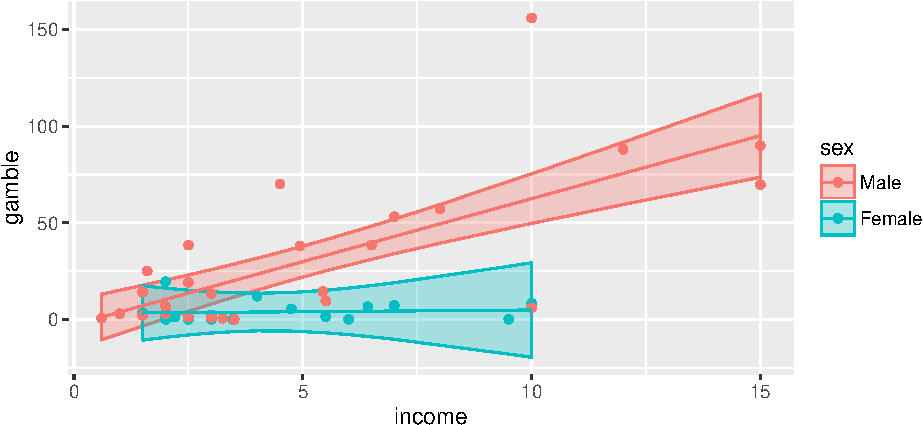
\includegraphics{Statistical_Methods_II_files/figure-latex/unnamed-chunk-45-1.pdf}

We will now see how to go about fitting these two models. As might be
imagined, these can be fit in the same fashion we have been solving the
linear models, but require a little finesse in defining the appropriate
design matrix \(\boldsymbol{X}\).

\section{Offset parallel Lines (aka additive
models)}\label{offset-parallel-lines-aka-additive-models}

In order to get offset parallel lines, we want to write a model
\[y_{i}=\begin{cases}
\beta_{0}+\beta_{1}+\beta_{2}x_{i}+\epsilon_{i} & \;\;\;\textrm{if female}\\
\beta_{0}+\beta_{2}x_{i}+\epsilon_{i} & \;\;\;\textrm{if male}
\end{cases}\] where \(\beta_{1}\) is the vertical offset of the female
group regression line to the reference group, which is the males
regression line. Because the first \(19\) observations are female, we
can this in in matrix form as \[\left[\begin{array}{c}
y_{1}\\
\vdots\\
y_{19}\\
y_{20}\\
\vdots\\
y_{47}
\end{array}\right]=\left[\begin{array}{ccc}
1 & 1 & x_{1}\\
\vdots & \vdots & \vdots\\
1 & 1 & x_{19}\\
1 & 0 & x_{20}\\
\vdots & \vdots & \vdots\\
1 & 0 & x_{47}
\end{array}\right]\left[\begin{array}{c}
\beta_{0}\\
\beta_{1}\\
\beta_{2}
\end{array}\right]+\left[\begin{array}{c}
\epsilon_{1}\\
\vdots\\
\epsilon_{19}\\
\epsilon_{20}\\
\vdots\\
\epsilon_{47}
\end{array}\right]\]

I like this representation where \(\beta_{1}\) is the offset from the
male regression line because it makes it very convenient to test if the
offset is equal to zero. The second column of the design matrix referred
to as a ``dummy variable'' or ``indicator variable'' that codes for the
female gender. Notice that even though I have two genders, I only had to
add one additional variable to my model because we already had a
y-intercept \(\beta_{0}\) and we only added one indicator variable for
females.

What if we had a third group? Then we would fit another column of
indicator variable for the third group. The new beta coefficient in the
model would be the offset of the new group to the reference group. For
example we consider \(n=9\) observations with \(n_i=3\) observations per
group where \(y_{i,j}\)is the \(j\) th replication of the \(i\)th group.
\[\left[\begin{array}{c}
y_{1,1}\\
y_{1,2}\\
y_{1,3}\\
y_{2,1}\\
y_{2,2}\\
y_{2,3}\\
y_{3,1}\\
y_{3,2}\\
y_{3,3}
\end{array}\right]=\left[\begin{array}{cccc}
1 & 0 & 0 & x_{1,1}\\
1 & 0 & 0 & x_{1,2}\\
1 & 0 & 0 & x_{1,3}\\
1 & 1 & 0 & x_{2,1}\\
1 & 1 & 0 & x_{2,2}\\
1 & 1 & 0 & x_{2,3}\\
1 & 0 & 1 & x_{3,1}\\
1 & 0 & 1 & x_{3,2}\\
1 & 0 & 1 & x_{3,3}
\end{array}\right]\left[\begin{array}{c}
\beta_{0}\\
\beta_{1}\\
\beta_{2}\\
\beta_{3}
\end{array}\right]+\left[\begin{array}{c}
\epsilon_{1,1}\\
\epsilon_{1,2}\\
\epsilon_{1,3}\\
\epsilon_{2,1}\\
\epsilon_{2,2}\\
\epsilon_{2,3}\\
\epsilon_{3,3}\\
\epsilon_{3,2}\\
\epsilon_{3,3}
\end{array}\right]
\]

In this model, \(\beta_0\) is the y-intercept for group \(1\). The
paramter \(\beta_1\) is the vertical offset from the reference group
(group \(1\)) for the second group. Similarly \(\beta_2\) is the
vertical offset for group \(3\). All groups will share the same slope,
\(\beta_4\).

\section{Lines with different slopes (aka Interaction
model)}\label{lines-with-different-slopes-aka-interaction-model}

We can now include a discrete random variable and create regression
lines that are parallel, but often that is inappropriate, such as in the
teenage gambling dataset. We want to be able to fit a model that has
different slopes. \[y_{i}=\begin{cases}
\left(\beta_{0}+\beta_{1}\right)+\left(\beta_{2}+\beta_{3}\right)x_{i}+\epsilon_{i} & \;\;\;\textrm{if female}\\
\beta_{0}+\beta_{2}x_{i}+\epsilon_{i} & \;\;\;\textrm{if male}
\end{cases}
\] Where \(\beta_{1}\) is the offset in y-intercept of the female group
from the male group, and \(\beta_{3}\) is the offset in slope. Now our
matrix formula looks like

\[\left[\begin{array}{c}
y_{1}\\
\vdots\\
y_{19}\\
y_{20}\\
\vdots\\
y_{47}
\end{array}\right]=\left[\begin{array}{cccc}
1 & 1 & x_{1} & x_{1}\\
\vdots & \vdots & \vdots & \vdots\\
1 & 1 & x_{19} & x_{19}\\
1 & 0 & x_{20} & 0\\
\vdots & \vdots & \vdots & \vdots\\
1 & 0 & x_{47} & 0
\end{array}\right]\left[\begin{array}{c}
\beta_{0}\\
\beta_{1}\\
\beta_{2}\\
\beta_{3}
\end{array}\right]+\left[\begin{array}{c}
\epsilon_{1}\\
\vdots\\
\epsilon_{19}\\
\epsilon_{20}\\
\vdots\\
\epsilon_{47}
\end{array}\right]
\] where the new fourth column is the what I would get if I multiplied
the \(\boldsymbol{x}\) column element-wise with the dummy-variable
column. To fit this model in R we have

\begin{Shaded}
\begin{Highlighting}[]
\KeywordTok{library}\NormalTok{(ggplot2)}
\KeywordTok{library}\NormalTok{(faraway)}

\CommentTok{# Forces R to recognize that 0, 1 are categorical, also}
\CommentTok{# relabels the levels to something I understand.}
\NormalTok{teengamb$sex <-}\StringTok{ }\KeywordTok{factor}\NormalTok{(teengamb$sex, }\DataTypeTok{labels=}\KeywordTok{c}\NormalTok{(}\StringTok{'Male'}\NormalTok{,}\StringTok{'Female'}\NormalTok{)) }

\CommentTok{# Fit a linear model with the interaction of sex and income}
\CommentTok{# Interactions can be specified useing a colon :}
\NormalTok{m1 <-}\StringTok{ }\KeywordTok{lm}\NormalTok{( gamble ~}\StringTok{ }\NormalTok{sex +}\StringTok{ }\NormalTok{income +}\StringTok{ }\NormalTok{sex:income, }\DataTypeTok{data=}\NormalTok{teengamb )  }

\CommentTok{# R allows a shortcut for the prior definition}
\NormalTok{m1 <-}\StringTok{ }\KeywordTok{lm}\NormalTok{( gamble ~}\StringTok{ }\NormalTok{sex *}\StringTok{ }\NormalTok{income, }\DataTypeTok{data=}\NormalTok{teengamb )}

\CommentTok{# save the fit, lwr, upr values for each observation}
\CommentTok{# these are the yhat and CI }
\NormalTok{teengamb <-}\StringTok{ }\KeywordTok{cbind}\NormalTok{(teengamb, }\KeywordTok{predict}\NormalTok{(m1, }\DataTypeTok{interval=}\StringTok{'conf'}\NormalTok{))}

\CommentTok{# Make a nice plot that includes the regreesion line.}
\KeywordTok{ggplot}\NormalTok{(teengamb, }\KeywordTok{aes}\NormalTok{(}\DataTypeTok{x=}\NormalTok{income, }\DataTypeTok{col=}\NormalTok{sex, }\DataTypeTok{fill=}\NormalTok{sex)) +}\StringTok{ }
\StringTok{      }\KeywordTok{geom_ribbon}\NormalTok{(}\KeywordTok{aes}\NormalTok{(}\DataTypeTok{ymin=}\NormalTok{lwr, }\DataTypeTok{ymax=}\NormalTok{upr),}
                  \DataTypeTok{alpha=}\NormalTok{.}\DecValTok{3}\NormalTok{) +}\StringTok{   }\CommentTok{# how solid the layer is}
\StringTok{      }\KeywordTok{geom_point}\NormalTok{(}\KeywordTok{aes}\NormalTok{(}\DataTypeTok{y=}\NormalTok{gamble)) +}
\StringTok{      }\KeywordTok{geom_line}\NormalTok{(}\KeywordTok{aes}\NormalTok{(}\DataTypeTok{y=}\NormalTok{fit)) }
\end{Highlighting}
\end{Shaded}

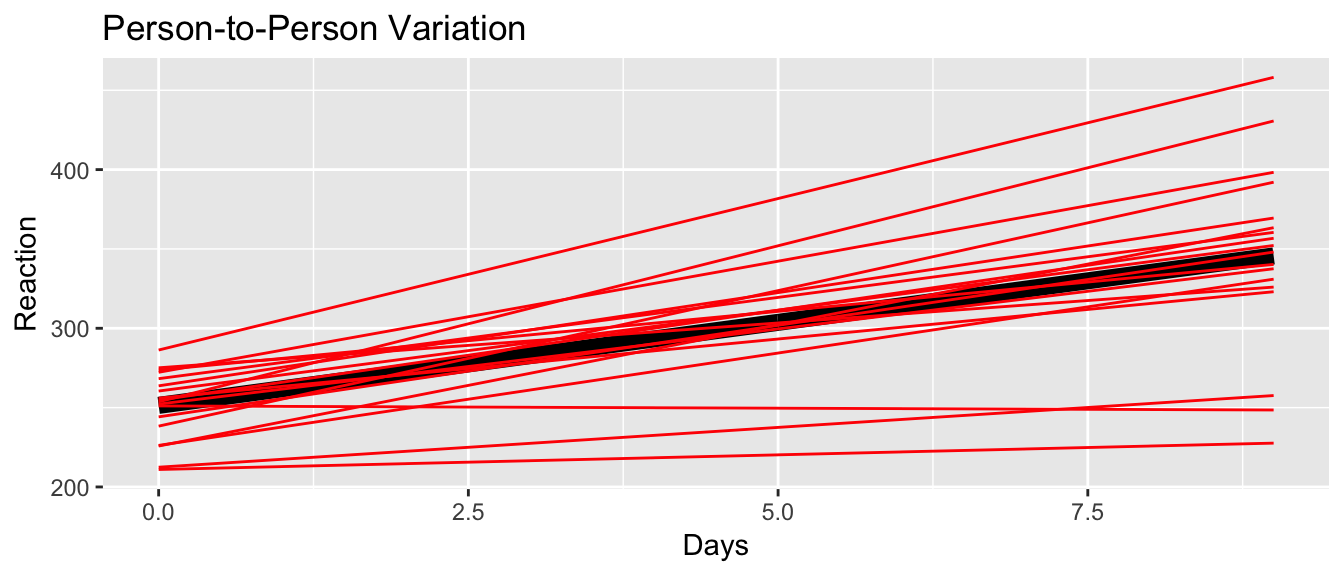
\includegraphics{Statistical_Methods_II_files/figure-latex/unnamed-chunk-46-1.pdf}

\begin{Shaded}
\begin{Highlighting}[]
\CommentTok{# print the model summary}
\KeywordTok{summary}\NormalTok{(m1)}
\end{Highlighting}
\end{Shaded}

\begin{verbatim}
## 
## Call:
## lm(formula = gamble ~ sex * income, data = teengamb)
## 
## Residuals:
##     Min      1Q  Median      3Q     Max 
## -56.522  -4.860  -1.790   6.273  93.478 
## 
## Coefficients:
##                  Estimate Std. Error t value Pr(>|t|)    
## (Intercept)       -2.6596     6.3164  -0.421  0.67580    
## sexFemale          5.7996    11.2003   0.518  0.60724    
## income             6.5181     0.9881   6.597 4.95e-08 ***
## sexFemale:income  -6.3432     2.1446  -2.958  0.00502 ** 
## ---
## Signif. codes:  0 '***' 0.001 '**' 0.01 '*' 0.05 '.' 0.1 ' ' 1
## 
## Residual standard error: 20.98 on 43 degrees of freedom
## Multiple R-squared:  0.5857, Adjusted R-squared:  0.5568 
## F-statistic: 20.26 on 3 and 43 DF,  p-value: 2.451e-08
\end{verbatim}

\section{Iris Example}\label{iris-example}

For a second example, we will explore the relationship between sepal
length and sepal width for three species of irises. This data set is
available in R as \texttt{iris}.

\begin{Shaded}
\begin{Highlighting}[]
\KeywordTok{data}\NormalTok{(iris)            }\CommentTok{# read in the iris dataset}
\KeywordTok{levels}\NormalTok{(iris$Species)  }\CommentTok{# notice the order of levels of Species}
\end{Highlighting}
\end{Shaded}

\begin{verbatim}
## [1] "setosa"     "versicolor" "virginica"
\end{verbatim}

The very first thing we should do when encountering a dataset is to do
some sort of graphical summary to get an idea of what model seems
appropriate.

\begin{Shaded}
\begin{Highlighting}[]
\KeywordTok{ggplot}\NormalTok{(iris, }\KeywordTok{aes}\NormalTok{(}\DataTypeTok{x=}\NormalTok{Sepal.Length, }\DataTypeTok{y=}\NormalTok{Sepal.Width, }\DataTypeTok{color=}\NormalTok{Species)) +}
\StringTok{  }\KeywordTok{geom_point}\NormalTok{()}
\end{Highlighting}
\end{Shaded}

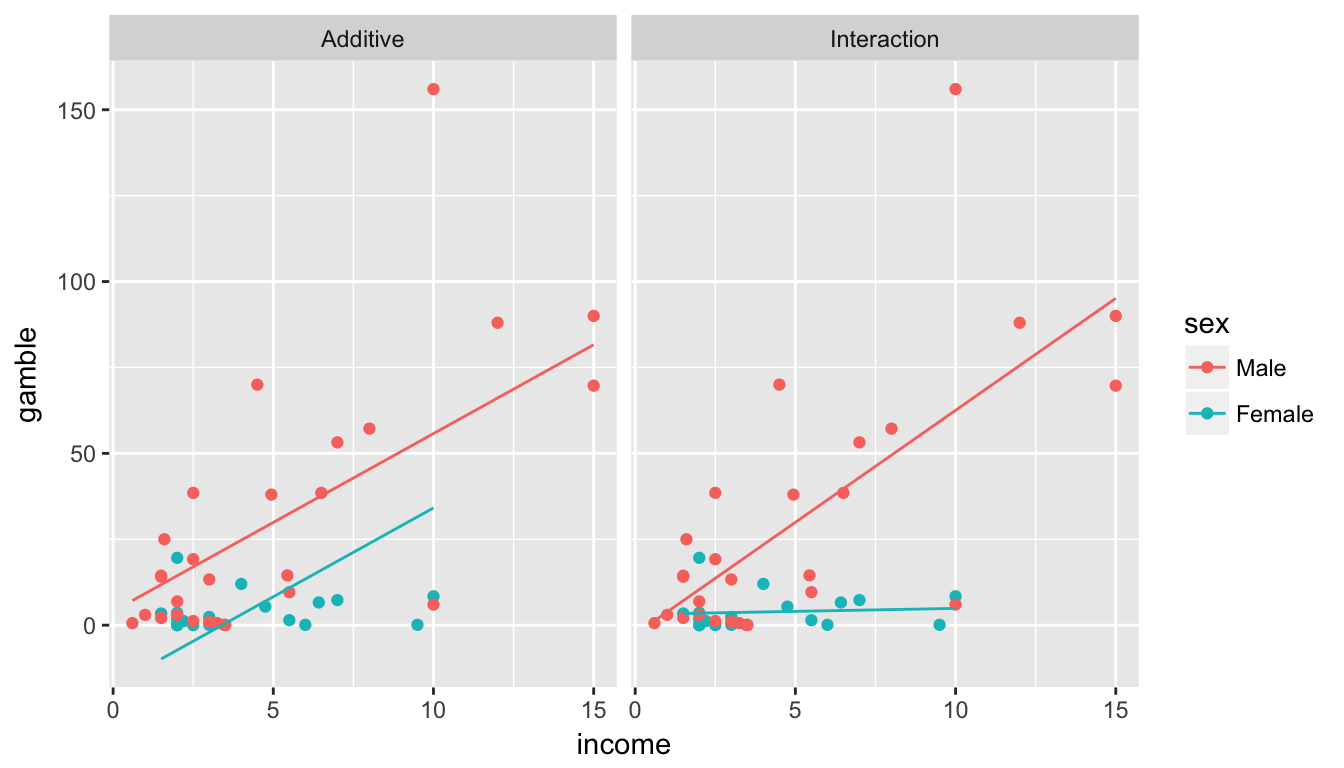
\includegraphics{Statistical_Methods_II_files/figure-latex/unnamed-chunk-48-1.pdf}

Looking at this graph, it seems that I will likely have a model with
different y-intercepts for each species, but it isn't clear to me if we
need different slopes.

We consider the sequence of building successively more complex models:

\begin{Shaded}
\begin{Highlighting}[]
\CommentTok{# make virginica the reference group }
\NormalTok{iris$Species <-}\StringTok{ }\KeywordTok{relevel}\NormalTok{(iris$Species, }\DataTypeTok{ref=}\StringTok{'virginica'}\NormalTok{)}

\NormalTok{m1 <-}\StringTok{ }\KeywordTok{lm}\NormalTok{( Sepal.Width ~}\StringTok{ }\NormalTok{Sepal.Length, }\DataTypeTok{data=}\NormalTok{iris )            }\CommentTok{# One line}
\NormalTok{m2 <-}\StringTok{ }\KeywordTok{lm}\NormalTok{( Sepal.Width ~}\StringTok{ }\NormalTok{Sepal.Length +}\StringTok{ }\NormalTok{Species, }\DataTypeTok{data=}\NormalTok{iris )  }\CommentTok{# Parallel Lines}
\NormalTok{m3 <-}\StringTok{ }\KeywordTok{lm}\NormalTok{( Sepal.Width ~}\StringTok{ }\NormalTok{Sepal.Length *}\StringTok{ }\NormalTok{Species, }\DataTypeTok{data=}\NormalTok{iris )  }\CommentTok{# Non-parallel Lines}
\end{Highlighting}
\end{Shaded}

The three models we consider are the following:

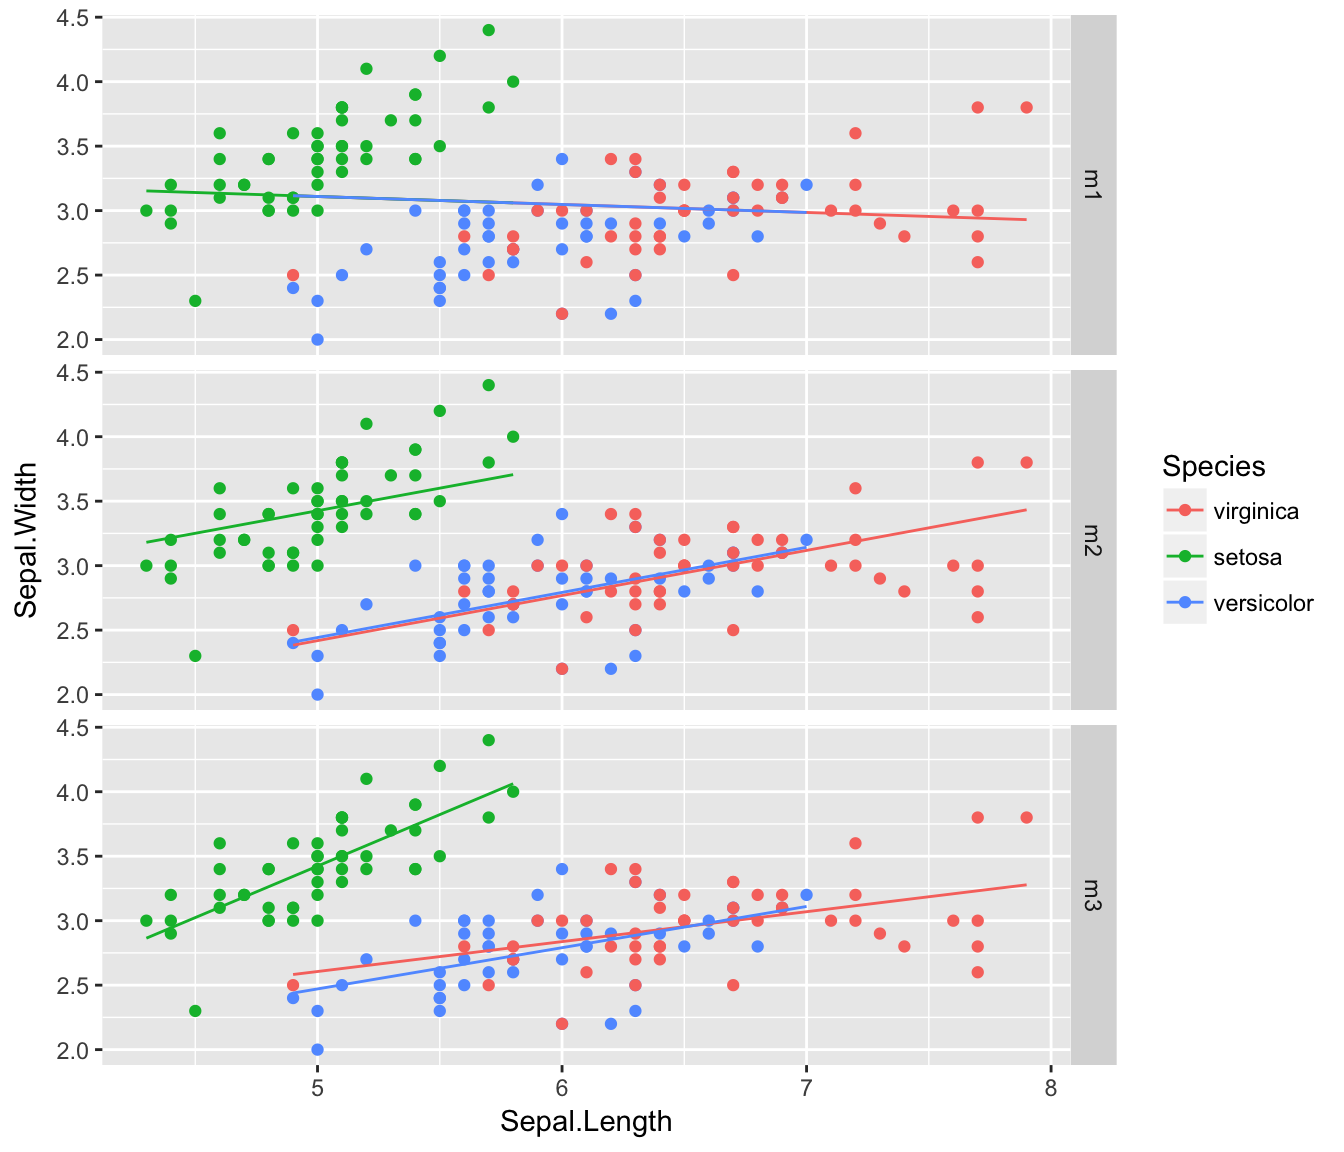
\includegraphics{Statistical_Methods_II_files/figure-latex/unnamed-chunk-50-1.pdf}

Looking at these, it seems obvious that the simplest model where we
ignore Species is horrible. The other two models seem decent, and I am
not sure about the parallel lines model vs the differing slopes model.

\begin{Shaded}
\begin{Highlighting}[]
\KeywordTok{summary}\NormalTok{(m1)$coefficients %>%}\StringTok{ }\KeywordTok{round}\NormalTok{(}\DataTypeTok{digits=}\DecValTok{3}\NormalTok{)  }
\end{Highlighting}
\end{Shaded}

\begin{verbatim}
##              Estimate Std. Error t value Pr(>|t|)
## (Intercept)     3.419      0.254  13.484    0.000
## Sepal.Length   -0.062      0.043  -1.440    0.152
\end{verbatim}

For the simplest model, there is so much unexplained noise that the
slope variable isn't significant.

Moving onto the next most complicated model, where each species has
their own y-intercept, but they share a slope, we have

\begin{Shaded}
\begin{Highlighting}[]
\KeywordTok{summary}\NormalTok{(m2)$coefficients %>%}\StringTok{ }\KeywordTok{round}\NormalTok{(}\DataTypeTok{digits=}\DecValTok{3}\NormalTok{)  }
\end{Highlighting}
\end{Shaded}

\begin{verbatim}
##                   Estimate Std. Error t value Pr(>|t|)
## (Intercept)          0.669      0.308   2.174    0.031
## Sepal.Length         0.350      0.046   7.557    0.000
## Speciessetosa        1.008      0.093  10.798    0.000
## Speciesversicolor    0.024      0.065   0.370    0.712
\end{verbatim}

The first two lines are the y-intercept and slope associated with the
reference group and the last two lines are the y-intercept offsets from
the reference group to \emph{Setosa} and \emph{Versicolor},
respectively. We have that the slope associated with increasing Sepal
Length is significant and that \emph{Setosa} has a statistically
different y-intercept than the reference group \emph{Virginica} and that
\emph{Versicolor} does not have a statstically different y-intercept
than the reference group.

Finally we consider the most complicated model that includes two more
slope parameters

\begin{Shaded}
\begin{Highlighting}[]
\KeywordTok{summary}\NormalTok{(m3)$coefficients %>%}\StringTok{ }\KeywordTok{round}\NormalTok{(}\DataTypeTok{digits=}\DecValTok{3}\NormalTok{)  }
\end{Highlighting}
\end{Shaded}

\begin{verbatim}
##                                Estimate Std. Error t value Pr(>|t|)
## (Intercept)                       1.446      0.405   3.572    0.000
## Sepal.Length                      0.232      0.061   3.790    0.000
## Speciessetosa                    -2.016      0.686  -2.938    0.004
## Speciesversicolor                -0.574      0.605  -0.950    0.344
## Sepal.Length:Speciessetosa        0.567      0.126   4.490    0.000
## Sepal.Length:Speciesversicolor    0.088      0.097   0.905    0.367
\end{verbatim}

These parameters are:

\begin{longtable}[]{@{}ll@{}}
\toprule
Meaning & R-label\tabularnewline
\midrule
\endhead
\emph{Reference group y-intercept } & (Intercept)\tabularnewline
\emph{Reference group slope } & Sepal.Length\tabularnewline
\emph{offset to y-intercept for Setosa} & Speciessetosa\tabularnewline
\emph{offset to y-intercept for Versicolor} &
Speciesversicolor\tabularnewline
\emph{offset to slope for Setosa} &
Sepal.Length:Speciessetosa\tabularnewline
\emph{offset to slope for Versicolor} &
Sepal.Length:Speciesversicolor\tabularnewline
\bottomrule
\end{longtable}

It appears that slope for \emph{Setosa} is different from the reference
group \emph{Virginica}. However because we've added \(2\) parameters to
the model, testing Model2 vs Model3 is not equivalent to just looking at
the p-value for that one slope. Instead we need to look at the F-test
comparing the two models which will evaluate if the decrease in SSE is
sufficient to justify the addition of two paramters.

\begin{Shaded}
\begin{Highlighting}[]
\KeywordTok{anova}\NormalTok{(m2, m3)}
\end{Highlighting}
\end{Shaded}

\begin{verbatim}
## Analysis of Variance Table
## 
## Model 1: Sepal.Width ~ Sepal.Length + Species
## Model 2: Sepal.Width ~ Sepal.Length * Species
##   Res.Df    RSS Df Sum of Sq      F   Pr(>F)    
## 1    146 12.193                                 
## 2    144 10.680  2    1.5132 10.201 7.19e-05 ***
## ---
## Signif. codes:  0 '***' 0.001 '**' 0.01 '*' 0.05 '.' 0.1 ' ' 1
\end{verbatim}

The F-test concludes that there is sufficent decrease in the SSE to
justify adding two additional parameters to the model.

\section{Exercises}\label{exercises-3}

\begin{enumerate}
\def\labelenumi{\arabic{enumi}.}
\tightlist
\item
  The in the \texttt{faraway} package, there is a dataset named
  \texttt{phbirths} that gives babies birth weights along with their
  gestational time in utero along with the mother's smoking status.

  \begin{enumerate}
  \def\labelenumii{\alph{enumii}.}
  \item
    Load and inspect the dataset using

\begin{Shaded}
\begin{Highlighting}[]
\KeywordTok{library}\NormalTok{(faraway)    }\CommentTok{# load the package}
\KeywordTok{data}\NormalTok{(phbirths)      }\CommentTok{# load the data within the package}
\NormalTok{?phbirths}
\end{Highlighting}
\end{Shaded}
  \item
    Create a plot of the birthweight vs the gestational age. Color code
    the points based on the mother's smoking status. Does it appear that
    smoking matters?
  \item
    Fit the simple model (one regression line) along with both the main
    effects (parallel lines) and interaction (non-parallel lines) ANCOVA
    model to these data. Which model is preferred?
  \item
    Using whichever model you selected in the previous section, create a
    graph of the data along with the confidence region for the
    regression line(s).
  \item
    Now consider only the ``full term babies'' which are babies with
    gestational age at birth \(\ge 36\) weeks. With this reduced
    dataset, repeat parts c,d.
  \item
    Interpret the relationship between gestational length and mother's
    smoking status on birthweight.
  \end{enumerate}
\item
  The in the \texttt{faraway} package, there is a dataset named
  \texttt{clot} that gives information about the time for blood to clot
  verses the blood dilution concentration when the blood was diluted
  with prothrombin-free plasma. Unfortunately the researchers had to
  order the plasma in two different lots (could think of this as two
  different sources) and need to assertain if the lot number makes any
  difference in clotting time.

  \begin{enumerate}
  \def\labelenumii{\alph{enumii}.}
  \tightlist
  \item
    Log transform the \texttt{time} and \texttt{conc} variable and plot
    the log-transformed data with color of the data point indicating the
    lot number.
  \item
    Ignoring the slight remaining curvature in the data, perform the
    appropriate analysis using transformed variables. Does \texttt{lot}
    matter?
  \end{enumerate}
\item
  In the \texttt{faraway} package, there is a data set
  \texttt{ToothGrowth} which is data from an experiment giving Vitamin C
  to guinea pigs. Guinea pigs were give vitamin C doses either via
  orange juice or ascorbic acid and the response of interest was a
  measure of tooth growth.

  \begin{enumerate}
  \def\labelenumii{\alph{enumii}.}
  \tightlist
  \item
    Log transform the \texttt{dose} and use that throughout this
    problem. Use \(e\) as the base, which R does by default when you use
    the \texttt{log()} function.
  \item
    Graph the data, fit appropriate ANCOVA models, and describe the
    relationship between the delivery method, log(dose) level, and tooth
    growth. Produce a graph with the data and the regression line(s)
    along with the confidence region for the line(s).
  \item
    Just using your graphs and visual inspection, at low dose levels,
    say \(\log(dose)=-0.7\), is there a difference in delivery method?
    What about at high dose levels, say \(\log(dose)=0.7\)? At this
    point we don't know how to answer this question using appropriate
    statistical inference, but we will address this in the chapter on
    contrasts.
  \end{enumerate}
\end{enumerate}

\chapter{Contrasts}\label{contrasts}

\begin{Shaded}
\begin{Highlighting}[]
\KeywordTok{library}\NormalTok{(ggplot2)}
\KeywordTok{library}\NormalTok{(dplyr)}
\KeywordTok{library}\NormalTok{(lsmeans)    }\CommentTok{# for lsmeans()}
\KeywordTok{library}\NormalTok{(multcomp)   }\CommentTok{# for glht() }
\end{Highlighting}
\end{Shaded}

We often are interested in estimating a function of the parameters
\(\boldsymbol{\beta}\). For example in the offset representation of the
ANOVA model with 3 groups we have \[y_{ij}=\mu+\tau_{i}+\epsilon_{ij}\]
where \[
\boldsymbol{\beta}=\left[\mu\;\tau_{2}\;\tau_{3}\right]^{T}
\] and \(\mu\) is the mean of the control group, group one is the
control group and thus \(\tau_{1}=0\), and \(\tau_{2}\) and \(\tau_{3}\)
are the offsets of group two and three from the control group. In this
representation, the mean of group two is \(\mu+\tau_{2}\) and is
estimated with \(\hat{\mu} + \hat{\tau}_2\).

\section{Estimate and variance}\label{estimate-and-variance}

A contrast is a linear combinations of elements of
\(\boldsymbol{\hat{\beta}}\), which is a fancy way of saying that it is
a function of the elements of \(\boldsymbol{\hat{\beta}}\) where the
elements can be added, subtracted, or multiplied by constants. In
particular, the contrast can be represented by the vector
\(\boldsymbol{c}\) such that the function we are interested in is
\(\boldsymbol{c}^{T}\boldsymbol{\hat{\beta}}\).

In the ANOVA case with \(k=3\) where we have the offset representation,
I might be interested in the mean of group 2, which could be written as
\[
\mu+\tau_{2}=\underset{\boldsymbol{c}^{T}}{\underbrace{\left[\begin{array}{ccc}
1 & 1 & 0\end{array}\right]}}\cdot\underset{\hat{\boldsymbol{\beta}}}{\underbrace{\left[\begin{array}{c}
\hat{\mu}\\
\hat{\tau_{2}}\\
\hat{\tau_{3}}
\end{array}\right]}}
\]

Similarly in the simple regression case, I will be interested in the
height of the regression line at \(x_0\). This height can be written
as\\
\[
\hat{\beta}_{0}+\hat{\beta}_{1}x_{0}=\underset{\boldsymbol{c}^{T}}{\underbrace{\left[\begin{array}{cc}
1 & x_{0}\end{array}\right]}}\cdot\underset{\hat{\boldsymbol{\beta}}}{\underbrace{\left[\begin{array}{c}
\hat{\beta}_{0}\\
\hat{\beta}_{1}
\end{array}\right]}}
\] In this manner, we could think of the predicted values \(\hat{y}_i\)
as just the result of the contrasts
\(\boldsymbol{X} \hat{\boldsymbol{\beta}}\) where our design matrix
takes the role of the contrasts.

One of the properties of maximum likelihood estimator (MLEs), is that
they are invariant under transformations. Meaning that since
\(\hat{\boldsymbol{\beta}}\) is the MLE of \(\boldsymbol{\beta}\), then
\(\boldsymbol{c}^{T}\hat{\boldsymbol{\beta}}\) is the MLE of
\(\boldsymbol{c}^{T}\boldsymbol{\beta}\). The only thing we need to
perform hypotheses tests and create confidence intervals is an estimate
of the variance of \(\boldsymbol{c}^{T}\hat{\boldsymbol{\beta}}\).

Because we know the variance of \(\hat{\boldsymbol{\beta}}\) is \[
Var\left(\hat{\boldsymbol{\beta}}\right)=\sigma^{2}\left(\boldsymbol{X}^{T}\boldsymbol{X}\right)^{-1}
\] and because \(\boldsymbol{c}\) is a constant, then \[
Var\left(\boldsymbol{c}^{T}\hat{\boldsymbol{\beta}}\right)=\sigma^{2}\boldsymbol{c}^{T}\left(\boldsymbol{X}^{T}\boldsymbol{X}\right)^{-1}\boldsymbol{c}
\] and the standard error is found by plugging in our estimate of
\(\sigma^{2}\) and taking the square root. \[
StdErr\left(\boldsymbol{c}^{T}\hat{\boldsymbol{\beta}}\right)   =   \sqrt{\hat{\sigma}^{2}\boldsymbol{c}^{T}\left(\boldsymbol{X}^{T}\boldsymbol{X}\right)^{-1}\boldsymbol{c}}
    =   \hat{\sigma}\sqrt{\boldsymbol{c}^{T}\left(\boldsymbol{X}^{T}\boldsymbol{X}\right)^{-1}\boldsymbol{c}}
\]

As usual, we can now calculate confidence intervals for
\(\boldsymbol{c}^{T}\hat{\boldsymbol{\beta}}\) using the usual formula
\[Est   \pm t_{n-p}^{1-\alpha/2}\;StdErr\left(\,Est\,\right)\] \[
\boldsymbol{c}^{T}\hat{\boldsymbol{\beta}}  \pm t_{n-p}^{1-\alpha/2}\;\hat{\sigma}\sqrt{\boldsymbol{c}^{T}\left(\boldsymbol{X}^{T}\boldsymbol{X}\right)^{-1}\boldsymbol{c}}
\]

Recall the hostility example which was an ANOVA with three groups with
the data

\begin{longtable}[]{@{}ll@{}}
\toprule
Method & Test Scores\tabularnewline
\midrule
\endhead
1 & 96 79 91 85 83 91 82 87\tabularnewline
2 & 77 76 74 73 78 71 80\tabularnewline
3 & 66 73 69 66 77 73 71 70 74\tabularnewline
\bottomrule
\end{longtable}

We have analyzed this data using both the cell means model and the
offset and we will demonstrate how to calculate the group means from the
offset representation. Thus we are interested in estimating
\(\mu+\tau_{2}\) and \(\mu+\tau_{3}\). I am also interested in
estimating the difference between treatment 2 and 3 and will therefore
be interested in estimating \(\tau_{2} - \tau_{3}\).

\begin{Shaded}
\begin{Highlighting}[]
\NormalTok{y <-}\StringTok{ }\KeywordTok{c}\NormalTok{(}\DecValTok{96}\NormalTok{,}\DecValTok{79}\NormalTok{,}\DecValTok{91}\NormalTok{,}\DecValTok{85}\NormalTok{,}\DecValTok{83}\NormalTok{,}\DecValTok{91}\NormalTok{,}\DecValTok{82}\NormalTok{,}\DecValTok{87}\NormalTok{,}
       \DecValTok{77}\NormalTok{,}\DecValTok{76}\NormalTok{,}\DecValTok{74}\NormalTok{,}\DecValTok{73}\NormalTok{,}\DecValTok{78}\NormalTok{,}\DecValTok{71}\NormalTok{,}\DecValTok{80}\NormalTok{,}
       \DecValTok{66}\NormalTok{,}\DecValTok{73}\NormalTok{,}\DecValTok{69}\NormalTok{,}\DecValTok{66}\NormalTok{,}\DecValTok{77}\NormalTok{,}\DecValTok{73}\NormalTok{,}\DecValTok{71}\NormalTok{,}\DecValTok{70}\NormalTok{,}\DecValTok{74}\NormalTok{)}
\NormalTok{groups <-}\StringTok{ }\KeywordTok{factor}\NormalTok{(}\KeywordTok{c}\NormalTok{( }\KeywordTok{rep}\NormalTok{(}\StringTok{'Group1'}\NormalTok{,}\DecValTok{8}\NormalTok{), }\KeywordTok{rep}\NormalTok{(}\StringTok{'Group2'}\NormalTok{,}\DecValTok{7}\NormalTok{),}\KeywordTok{rep}\NormalTok{(}\StringTok{'Group3'}\NormalTok{,}\DecValTok{9}\NormalTok{) ))}
\end{Highlighting}
\end{Shaded}

We can fit the offset model and obtain the design matrix and estimate of
\(\hat{\sigma}\) via the following code.

\begin{Shaded}
\begin{Highlighting}[]
\NormalTok{m <-}\StringTok{ }\KeywordTok{lm}\NormalTok{(y ~}\StringTok{ }\NormalTok{groups)            }\CommentTok{# Fit the ANOVA model (offset representation)}
\KeywordTok{coef}\NormalTok{(m)                        }\CommentTok{# Show me beta.hat}
\end{Highlighting}
\end{Shaded}

\begin{verbatim}
##  (Intercept) groupsGroup2 groupsGroup3 
##     86.75000    -11.17857    -15.75000
\end{verbatim}

\begin{Shaded}
\begin{Highlighting}[]
\NormalTok{X <-}\StringTok{ }\KeywordTok{model.matrix}\NormalTok{(m)           }\CommentTok{# obtains the design matrix}
\NormalTok{sigma.hat <-}\StringTok{ }\KeywordTok{summary}\NormalTok{(m)$sigma  }\CommentTok{# create the summary table and grab sigma.hat }
\NormalTok{beta.hat <-}\StringTok{ }\KeywordTok{coef}\NormalTok{(m)}
\NormalTok{XtX.inv <-}\StringTok{ }\KeywordTok{solve}\NormalTok{( }\KeywordTok{t}\NormalTok{(X) %*%}\StringTok{ }\NormalTok{X )}
\end{Highlighting}
\end{Shaded}

Now we calculate

\begin{Shaded}
\begin{Highlighting}[]
\NormalTok{contr <-}\StringTok{ }\KeywordTok{c}\NormalTok{(}\DecValTok{1}\NormalTok{,}\DecValTok{1}\NormalTok{,}\DecValTok{0}\NormalTok{)  }\CommentTok{# define my contrast}
\NormalTok{ctb <-}\StringTok{ }\KeywordTok{t}\NormalTok{(contr) %*%}\StringTok{ }\NormalTok{beta.hat}
\NormalTok{std.err <-}\StringTok{ }\NormalTok{sigma.hat *}\StringTok{ }\KeywordTok{sqrt}\NormalTok{( }\KeywordTok{t}\NormalTok{(contr) %*%}\StringTok{ }\NormalTok{XtX.inv %*%}\StringTok{ }\NormalTok{contr )}
\NormalTok{ctb}
\end{Highlighting}
\end{Shaded}

\begin{verbatim}
##          [,1]
## [1,] 75.57143
\end{verbatim}

\begin{Shaded}
\begin{Highlighting}[]
\NormalTok{std.err}
\end{Highlighting}
\end{Shaded}

\begin{verbatim}
##          [,1]
## [1,] 1.622994
\end{verbatim}

and notice this is the exact same estimate and standard error we got for
group two when we fit the cell means model.

\begin{Shaded}
\begin{Highlighting}[]
\NormalTok{CellMeansModel <-}\StringTok{ }\KeywordTok{lm}\NormalTok{(y ~}\StringTok{ }\NormalTok{groups -}\StringTok{ }\DecValTok{1}\NormalTok{)}
\KeywordTok{summary}\NormalTok{(CellMeansModel)$coefficients}
\end{Highlighting}
\end{Shaded}

\begin{verbatim}
##              Estimate Std. Error  t value     Pr(>|t|)
## groupsGroup1 86.75000   1.518172 57.14108 1.567052e-24
## groupsGroup2 75.57143   1.622994 46.56296 1.117034e-22
## groupsGroup3 71.00000   1.431347 49.60364 2.993023e-23
\end{verbatim}

\section{\texorpdfstring{Estimating contrasts using
\texttt{glht()}}{Estimating contrasts using glht()}}\label{estimating-contrasts-using-glht}

Instead of us doing all the matrix calculations ourselves, all we really
need is to is specify the row vector \(\boldsymbol{c}^{T}\). The
function that will do the rest of the calculations is the generalized
linear hypothesis test function \texttt{glht()} that can be found in the
multiple comparisons package \texttt{multcomp}. The p-values will be
adjusted to correct for testing multiple hypothesis, so there may be
slight differences compared to the p-value seen in just the regular
summary table.

\subsection{1-way ANOVA}\label{way-anova}

We will again use the Hostility data set and demonstrate how to
calculate the point estimates, standard errors and confidence intervals
for the group means given a model fit using the offset representation.

\begin{Shaded}
\begin{Highlighting}[]
\NormalTok{y <-}\StringTok{ }\KeywordTok{c}\NormalTok{(}\DecValTok{96}\NormalTok{,}\DecValTok{79}\NormalTok{,}\DecValTok{91}\NormalTok{,}\DecValTok{85}\NormalTok{,}\DecValTok{83}\NormalTok{,}\DecValTok{91}\NormalTok{,}\DecValTok{82}\NormalTok{,}\DecValTok{87}\NormalTok{,}
       \DecValTok{77}\NormalTok{,}\DecValTok{76}\NormalTok{,}\DecValTok{74}\NormalTok{,}\DecValTok{73}\NormalTok{,}\DecValTok{78}\NormalTok{,}\DecValTok{71}\NormalTok{,}\DecValTok{80}\NormalTok{,}
       \DecValTok{66}\NormalTok{,}\DecValTok{73}\NormalTok{,}\DecValTok{69}\NormalTok{,}\DecValTok{66}\NormalTok{,}\DecValTok{77}\NormalTok{,}\DecValTok{73}\NormalTok{,}\DecValTok{71}\NormalTok{,}\DecValTok{70}\NormalTok{,}\DecValTok{74}\NormalTok{)}
\NormalTok{groups <-}\StringTok{ }\KeywordTok{factor}\NormalTok{(}\KeywordTok{c}\NormalTok{( }\KeywordTok{rep}\NormalTok{(}\StringTok{'Group1'}\NormalTok{,}\DecValTok{8}\NormalTok{), }\KeywordTok{rep}\NormalTok{(}\StringTok{'Group2'}\NormalTok{,}\DecValTok{7}\NormalTok{),}\KeywordTok{rep}\NormalTok{(}\StringTok{'Group3'}\NormalTok{,}\DecValTok{9}\NormalTok{) ))}
\NormalTok{m <-}\StringTok{ }\KeywordTok{lm}\NormalTok{(y ~}\StringTok{ }\NormalTok{groups)}
\KeywordTok{summary}\NormalTok{(m)$coefficients}
\end{Highlighting}
\end{Shaded}

\begin{verbatim}
##               Estimate Std. Error   t value     Pr(>|t|)
## (Intercept)   86.75000   1.518172 57.141079 1.567052e-24
## groupsGroup2 -11.17857   2.222377 -5.030008 5.583942e-05
## groupsGroup3 -15.75000   2.086528 -7.548424 2.063600e-07
\end{verbatim}

We will now define a row vector (and it needs to be a matrix or else
\texttt{glht()} will throw an error. First we note that the simple
contrast \(\boldsymbol{c}^{T}=\left[1\;0\;0\right]\) just grabs the
first coefficient and gives us the same estimate and standard error as
the summary did.

\begin{Shaded}
\begin{Highlighting}[]
\KeywordTok{library}\NormalTok{(multcomp)}
\NormalTok{contr <-}\StringTok{ }\KeywordTok{rbind}\NormalTok{(}\StringTok{"Intercept"}\NormalTok{=}\KeywordTok{c}\NormalTok{(}\DecValTok{1}\NormalTok{,}\DecValTok{0}\NormalTok{,}\DecValTok{0}\NormalTok{)) }\CommentTok{# 1x3 matrix with row named "Intercept"}
\NormalTok{test <-}\StringTok{ }\KeywordTok{glht}\NormalTok{(m, }\DataTypeTok{linfct=}\NormalTok{contr)        }\CommentTok{# the linear function to be tested is contr}
\KeywordTok{summary}\NormalTok{(test)}
\end{Highlighting}
\end{Shaded}

\begin{verbatim}
## 
##   Simultaneous Tests for General Linear Hypotheses
## 
## Fit: lm(formula = y ~ groups)
## 
## Linear Hypotheses:
##                Estimate Std. Error t value Pr(>|t|)    
## Intercept == 0   86.750      1.518   57.14   <2e-16 ***
## ---
## Signif. codes:  0 '***' 0.001 '**' 0.01 '*' 0.05 '.' 0.1 ' ' 1
## (Adjusted p values reported -- single-step method)
\end{verbatim}

Next we calculate the estimate of all the group means \(\mu\),
\(\mu+\tau_{2}\) and \(\mu+\tau_{3}\) and the difference between group 2
and 3. Notice I can specify more than one contrast at a time.

\begin{Shaded}
\begin{Highlighting}[]
\NormalTok{contr <-}\StringTok{ }\KeywordTok{rbind}\NormalTok{(}\StringTok{"Mean of Group 1"}\NormalTok{=}\KeywordTok{c}\NormalTok{(}\DecValTok{1}\NormalTok{,}\DecValTok{0}\NormalTok{,}\DecValTok{0}\NormalTok{),}
               \StringTok{"Mean of Group 2"}\NormalTok{=}\KeywordTok{c}\NormalTok{(}\DecValTok{1}\NormalTok{,}\DecValTok{1}\NormalTok{,}\DecValTok{0}\NormalTok{),}
               \StringTok{"Mean of Group 3"}\NormalTok{=}\KeywordTok{c}\NormalTok{(}\DecValTok{1}\NormalTok{,}\DecValTok{0}\NormalTok{,}\DecValTok{1}\NormalTok{),}
               \StringTok{"Diff G2-G3"}     \NormalTok{=}\KeywordTok{c}\NormalTok{(}\DecValTok{0}\NormalTok{,}\DecValTok{1}\NormalTok{,-}\DecValTok{1}\NormalTok{)) }
\NormalTok{test <-}\StringTok{ }\KeywordTok{glht}\NormalTok{(m, }\DataTypeTok{linfct=}\NormalTok{contr)}
\KeywordTok{summary}\NormalTok{(test)}
\end{Highlighting}
\end{Shaded}

\begin{verbatim}
## 
##   Simultaneous Tests for General Linear Hypotheses
## 
## Fit: lm(formula = y ~ groups)
## 
## Linear Hypotheses:
##                      Estimate Std. Error t value Pr(>|t|)    
## Mean of Group 1 == 0   86.750      1.518  57.141   <1e-04 ***
## Mean of Group 2 == 0   75.571      1.623  46.563   <1e-04 ***
## Mean of Group 3 == 0   71.000      1.431  49.604   <1e-04 ***
## Diff G2-G3 == 0         4.571      2.164   2.112    0.144    
## ---
## Signif. codes:  0 '***' 0.001 '**' 0.01 '*' 0.05 '.' 0.1 ' ' 1
## (Adjusted p values reported -- single-step method)
\end{verbatim}

Finally we calculate confidence intervals in the usual manner using the
\texttt{confint()} function.

\begin{Shaded}
\begin{Highlighting}[]
\KeywordTok{confint}\NormalTok{(test, }\DataTypeTok{level=}\FloatTok{0.95}\NormalTok{)}
\end{Highlighting}
\end{Shaded}

\begin{verbatim}
## 
##   Simultaneous Confidence Intervals
## 
## Fit: lm(formula = y ~ groups)
## 
## Quantile = 2.6455
## 95% family-wise confidence level
##  
## 
## Linear Hypotheses:
##                      Estimate lwr     upr    
## Mean of Group 1 == 0 86.7500  82.7337 90.7663
## Mean of Group 2 == 0 75.5714  71.2778 79.8651
## Mean of Group 3 == 0 71.0000  67.2134 74.7866
## Diff G2-G3 == 0       4.5714  -1.1534 10.2963
\end{verbatim}

\subsection{ANCOVA example}\label{ancova-example}

In the ANCOVA case, there are more interesting contrasts to be made. For
this example we will use the \texttt{ToothGrowth} dataset. This data
measuring the effects of different dose levels of vitamin C on tooth
growth of guinea pigs. The two different delivery methods are encoded by
the variable supp which has levels of orange juice (OJ) and ascorbic
acid (VC).

We first fit a ANCOVA model with an interaction between log(dose) level
and delivery method and graph the result.

\begin{Shaded}
\begin{Highlighting}[]
\KeywordTok{data}\NormalTok{(}\StringTok{'ToothGrowth'}\NormalTok{)}
\NormalTok{ToothGrowth$logDose <-}\StringTok{ }\KeywordTok{log}\NormalTok{( ToothGrowth$dose )}
\NormalTok{m <-}\StringTok{ }\KeywordTok{lm}\NormalTok{(len ~}\StringTok{ }\NormalTok{logDose *}\StringTok{ }\NormalTok{supp, }\DataTypeTok{data=}\NormalTok{ToothGrowth)}

\CommentTok{# predict() gives me the yhat values and optional CI}
\CommentTok{# these are just the "contrasts" defined by X matrix! }
\NormalTok{ToothGrowth$len.hat <-}\StringTok{ }\KeywordTok{predict}\NormalTok{(m, }\DataTypeTok{interval=}\StringTok{'confidence'}\NormalTok{)[,}\DecValTok{1}\NormalTok{]}
\NormalTok{ToothGrowth$len.lwr <-}\StringTok{ }\KeywordTok{predict}\NormalTok{(m, }\DataTypeTok{interval=}\StringTok{'confidence'}\NormalTok{)[,}\DecValTok{2}\NormalTok{]}
\NormalTok{ToothGrowth$len.upr <-}\StringTok{ }\KeywordTok{predict}\NormalTok{(m, }\DataTypeTok{interval=}\StringTok{'confidence'}\NormalTok{)[,}\DecValTok{3}\NormalTok{]}

\CommentTok{# Plot the results using ggplot2}
\KeywordTok{ggplot}\NormalTok{( ToothGrowth, }\KeywordTok{aes}\NormalTok{(}\DataTypeTok{x=}\NormalTok{logDose, }\DataTypeTok{col=}\NormalTok{supp, }\DataTypeTok{fill=}\NormalTok{supp)) +}
\StringTok{    }\KeywordTok{geom_point}\NormalTok{(}\KeywordTok{aes}\NormalTok{(}\DataTypeTok{y=}\NormalTok{len)) +}
\StringTok{    }\KeywordTok{geom_line}\NormalTok{(}\KeywordTok{aes}\NormalTok{(}\DataTypeTok{y=}\NormalTok{len.hat)) +}
\StringTok{    }\KeywordTok{geom_ribbon}\NormalTok{(}\KeywordTok{aes}\NormalTok{(}\DataTypeTok{ymin=}\NormalTok{len.lwr, }\DataTypeTok{ymax=}\NormalTok{len.upr), }\DataTypeTok{alpha=}\NormalTok{.}\DecValTok{2}\NormalTok{)}
\end{Highlighting}
\end{Shaded}

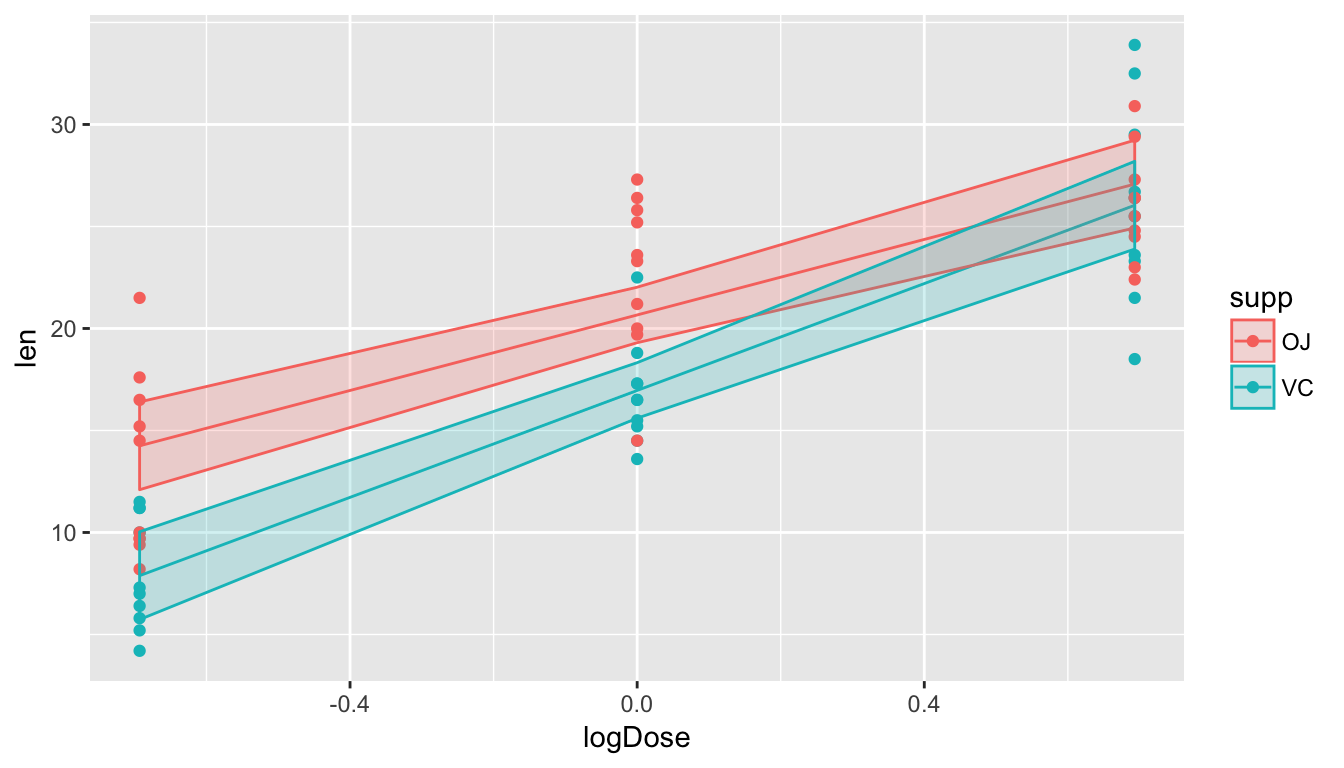
\includegraphics{Statistical_Methods_II_files/figure-latex/unnamed-chunk-66-1.pdf}

R has fit this model using the offset representation. First we present
the summary coefficients so we know which parameters are which.

\begin{Shaded}
\begin{Highlighting}[]
\KeywordTok{summary}\NormalTok{(m)$coefficient}
\end{Highlighting}
\end{Shaded}

\begin{verbatim}
##                 Estimate Std. Error   t value     Pr(>|t|)
## (Intercept)    20.663333  0.6791481 30.425371 1.629404e-36
## logDose         9.254889  1.2000095  7.712346 2.302639e-10
## suppVC         -3.700000  0.9604605 -3.852319 3.033467e-04
## logDose:suppVC  3.844782  1.6970696  2.265542 2.736578e-02
\end{verbatim}

For a warm-up, we will calculate the y-intercepts of both groups and the
slopes of both. For the OJ group, this is just the 1st and 2nd
coefficients, while for the VC group it is \(\beta_{0}+\beta_{2}\) and
\(\beta_{1}+\beta_{3}\).

\begin{Shaded}
\begin{Highlighting}[]
\CommentTok{# Add a heading so that I know which parameter is which!}
\CommentTok{#                                Int  logDose  suppVC   logDose:suppVC}
\NormalTok{contr <-}\StringTok{ }\KeywordTok{rbind}\NormalTok{(}\StringTok{"Intercept OJ"} \NormalTok{=}\StringTok{ }\KeywordTok{c}\NormalTok{(}\DecValTok{1}\NormalTok{,     }\DecValTok{0}\NormalTok{,     }\DecValTok{0}\NormalTok{,          }\DecValTok{0}          \NormalTok{),}
               \StringTok{"Slope     OJ"} \NormalTok{=}\StringTok{ }\KeywordTok{c}\NormalTok{(}\DecValTok{0}\NormalTok{,     }\DecValTok{1}\NormalTok{,     }\DecValTok{0}\NormalTok{,          }\DecValTok{0}          \NormalTok{),}
               \StringTok{"Intercept VC"} \NormalTok{=}\StringTok{ }\KeywordTok{c}\NormalTok{(}\DecValTok{1}\NormalTok{,     }\DecValTok{0}\NormalTok{,     }\DecValTok{1}\NormalTok{,          }\DecValTok{0}          \NormalTok{),}
               \StringTok{"Slope     VC"} \NormalTok{=}\StringTok{ }\KeywordTok{c}\NormalTok{(}\DecValTok{0}\NormalTok{,     }\DecValTok{1}\NormalTok{,     }\DecValTok{0}\NormalTok{,          }\DecValTok{1}          \NormalTok{) ) }
\NormalTok{test <-}\StringTok{ }\KeywordTok{glht}\NormalTok{(m, }\DataTypeTok{linfct=}\NormalTok{contr)}
\KeywordTok{summary}\NormalTok{(test)}
\end{Highlighting}
\end{Shaded}

\begin{verbatim}
## 
##   Simultaneous Tests for General Linear Hypotheses
## 
## Fit: lm(formula = len ~ logDose * supp, data = ToothGrowth)
## 
## Linear Hypotheses:
##                   Estimate Std. Error t value Pr(>|t|)    
## Intercept OJ == 0  20.6633     0.6791  30.425   <1e-09 ***
## Slope     OJ == 0   9.2549     1.2000   7.712   <1e-09 ***
## Intercept VC == 0  16.9633     0.6791  24.977   <1e-09 ***
## Slope     VC == 0  13.0997     1.2000  10.916   <1e-09 ***
## ---
## Signif. codes:  0 '***' 0.001 '**' 0.01 '*' 0.05 '.' 0.1 ' ' 1
## (Adjusted p values reported -- single-step method)
\end{verbatim}

In our original table of summary coefficients, the (intercept) term
corresponds to the tooth growth of a guinea pig when the logDose level
is 0 (and therefore dose=1). If I wanted to estimate the tooth growth of
a guinea pig fed OJ but with only \(1/2\) a dose (and therefore
\(logDose=\log\left(1/2\right)=-0.69\)), then we want

\[\begin{aligned}
\hat{y}_{oj,dose=0.5}   & =     \hat{\beta}_{0}+\hat{\beta}_{1}\log\left(0.5\right)\\
                        & =     20.6+9.25\log\left(0.5\right)\\
                        & =     20.6+9.25\left(-0.69\right)\\
                        & =     14.21
\end{aligned}\]

which I can write as \[y_{oj,dose=0.5}   =   \left[\begin{array}{cccc}
1 & -0.69 & 0 & 0\end{array}\right]\left[\begin{array}{c}
\hat{\beta_{0}}\\
\hat{\beta}_{1}\\
\hat{\beta}_{2}\\
\hat{\beta}_{3}
\end{array}\right]
    =   \boldsymbol{c}_{1}^{T}\hat{\boldsymbol{\beta}}\]

To calculate the same value for the VC group, we need the following
contrast:

\[\begin{aligned}
\hat{y}_{vc,dose=0.5}   
    &=  16.9633+13.0997\,\log\left(0.5\right)\\
    &=  \left(20.66-3.7\right)+\left(9.25+3.8\right)\,\log\left(0.5\right)\\
      &=    \left(\hat{\beta}_{0}+\hat{\beta}_{2}\right)+\left(\hat{\beta}_{1}+\hat{\beta}_{3}\right)\,\left(-0.69\right)\\
      &=    \left[\begin{array}{cccc}1 & -0.69 & 1 & -0.69\end{array}\right]\left[\begin{array}{c}
                 \hat{\beta_{0}}\\
                 \hat{\beta}_{1}\\
                 \hat{\beta}_{2}\\
                 \hat{\beta}_{3}\end{array}\right]\\
      &=    \boldsymbol{c}_{2}^{T}\hat{\boldsymbol{\beta}}
      \end{aligned}\]

\begin{Shaded}
\begin{Highlighting}[]
\CommentTok{#                                Int  logDose  suppVC   logDose:suppVC}
\NormalTok{contr <-}\StringTok{ }\KeywordTok{rbind}\NormalTok{(}\StringTok{"OJ; 1/2 dose"} \NormalTok{=}\StringTok{ }\KeywordTok{c}\NormalTok{(}\DecValTok{1}\NormalTok{,   -}\FloatTok{0.69}\NormalTok{,    }\DecValTok{0}\NormalTok{,          }\DecValTok{0}         \NormalTok{),}
               \StringTok{"VC; 1/2 dose"} \NormalTok{=}\StringTok{ }\KeywordTok{c}\NormalTok{(}\DecValTok{1}\NormalTok{,   -}\FloatTok{0.69}\NormalTok{,    }\DecValTok{1}\NormalTok{,        -}\FloatTok{0.69}       \NormalTok{))}
\NormalTok{test <-}\StringTok{ }\KeywordTok{glht}\NormalTok{(m, }\DataTypeTok{linfct=}\NormalTok{contr)}
\KeywordTok{summary}\NormalTok{(test)}
\end{Highlighting}
\end{Shaded}

\begin{verbatim}
## 
##   Simultaneous Tests for General Linear Hypotheses
## 
## Fit: lm(formula = len ~ logDose * supp, data = ToothGrowth)
## 
## Linear Hypotheses:
##                   Estimate Std. Error t value Pr(>|t|)    
## OJ; 1/2 dose == 0   14.277      1.071   13.33  < 1e-10 ***
## VC; 1/2 dose == 0    7.925      1.071    7.40 1.51e-09 ***
## ---
## Signif. codes:  0 '***' 0.001 '**' 0.01 '*' 0.05 '.' 0.1 ' ' 1
## (Adjusted p values reported -- single-step method)
\end{verbatim}

Finally we might be interested in testing if there is a treatment
difference between OJ and VC at a 1/2 dose level. So to do this, we want
to calculate the difference between these two previous contrasts, i.e.

\[\begin{aligned}
\boldsymbol{c}_{1}^{T}\hat{\boldsymbol{\beta}}-\boldsymbol{c}_{2}^{T}\hat{\boldsymbol{\beta}}   &=  \left(\boldsymbol{c}_{1}^{T}-\boldsymbol{c}_{2}^{T}\right) \hat{\boldsymbol{ \beta }} \\
    &=  \left(\left[\begin{array}{cccc}
1 & -0.69 & 0 & 0\end{array}\right]-\left[\begin{array}{cccc}
1 & -0.69 & 1 & -0.69\end{array}\right]\right)\hat{\boldsymbol{\beta}} \\
    &=  \left[\begin{array}{cccc}
0 & 0 & -1 & 0.69\end{array}\right]\hat{\boldsymbol{\beta}}
\end{aligned}\]

and we can calculate

\begin{Shaded}
\begin{Highlighting}[]
\NormalTok{contr <-}\StringTok{ }\KeywordTok{rbind}\NormalTok{(}\StringTok{"OJ - VC; 1/2 dose"} \NormalTok{=}\StringTok{ }\KeywordTok{c}\NormalTok{(}\DecValTok{0}\NormalTok{, }\DecValTok{0}\NormalTok{, -}\DecValTok{1}\NormalTok{, }\FloatTok{0.69}\NormalTok{))}
\NormalTok{test <-}\StringTok{ }\KeywordTok{glht}\NormalTok{(m, }\DataTypeTok{linfct=}\NormalTok{contr)}
\KeywordTok{summary}\NormalTok{(test)}
\end{Highlighting}
\end{Shaded}

\begin{verbatim}
## 
##   Simultaneous Tests for General Linear Hypotheses
## 
## Fit: lm(formula = len ~ logDose * supp, data = ToothGrowth)
## 
## Linear Hypotheses:
##                        Estimate Std. Error t value Pr(>|t|)    
## OJ - VC; 1/2 dose == 0    6.353      1.514   4.195 9.83e-05 ***
## ---
## Signif. codes:  0 '***' 0.001 '**' 0.01 '*' 0.05 '.' 0.1 ' ' 1
## (Adjusted p values reported -- single-step method)
\end{verbatim}

When we do the same test, but at dose level 2 (logDose =\(\log2=0.69\))
we see that the difference is not statistically significant.

\begin{Shaded}
\begin{Highlighting}[]
\NormalTok{contr <-}\StringTok{ }\KeywordTok{rbind}\NormalTok{(}\StringTok{"OJ - VC; dose 2"} \NormalTok{=}\StringTok{ }\KeywordTok{c}\NormalTok{(}\DecValTok{0}\NormalTok{, }\DecValTok{0}\NormalTok{, -}\DecValTok{1}\NormalTok{, -}\FloatTok{0.69}\NormalTok{))}
\NormalTok{test <-}\StringTok{ }\KeywordTok{glht}\NormalTok{(m, }\DataTypeTok{linfct=}\NormalTok{contr)}
\KeywordTok{summary}\NormalTok{(test)}
\end{Highlighting}
\end{Shaded}

\begin{verbatim}
## 
##   Simultaneous Tests for General Linear Hypotheses
## 
## Fit: lm(formula = len ~ logDose * supp, data = ToothGrowth)
## 
## Linear Hypotheses:
##                      Estimate Std. Error t value Pr(>|t|)
## OJ - VC; dose 2 == 0    1.047      1.514   0.691    0.492
## (Adjusted p values reported -- single-step method)
\end{verbatim}

\section{\texorpdfstring{Using \texttt{lsmeans}
Package}{Using lsmeans Package}}\label{using-lsmeans-package}

Specifying the contrasts by hand is extremely difficult to do correctly
and instead we would prefer to specify the contrasts using language like
``create all possible pairwise contrasts'' where each pair is just a
subtraction. The R-package \texttt{lsmeans} tries to simply the creation
of common contrasts.

To show how to use the \texttt{lsmeans} package, we'll consider a bunch
of common models and show how to address common statistical questions
for each.

\subsection{Simple Regression}\label{simple-regression-1}

There is a dataset built into R named \texttt{trees} which describes a
set of \(n=31\) cherry trees and the goal is to predict the volume of
timber produced by each tree just using the tree girth a 4.5 feet above
the ground.

\begin{Shaded}
\begin{Highlighting}[]
\KeywordTok{data}\NormalTok{(trees)}
\NormalTok{model <-}\StringTok{ }\KeywordTok{lm}\NormalTok{( Volume ~}\StringTok{ }\NormalTok{Girth, }\DataTypeTok{data=}\NormalTok{trees )}
\NormalTok{trees <-}\StringTok{ }\KeywordTok{cbind}\NormalTok{( trees, }\KeywordTok{predict}\NormalTok{(model, }\DataTypeTok{interval=}\StringTok{'conf'}\NormalTok{))}
\KeywordTok{ggplot}\NormalTok{(trees, }\KeywordTok{aes}\NormalTok{(}\DataTypeTok{x=}\NormalTok{Girth, }\DataTypeTok{y=}\NormalTok{Volume)) +}
\StringTok{  }\KeywordTok{geom_point}\NormalTok{() +}
\StringTok{  }\KeywordTok{geom_ribbon}\NormalTok{( }\KeywordTok{aes}\NormalTok{(}\DataTypeTok{ymin=}\NormalTok{lwr, }\DataTypeTok{ymax=}\NormalTok{upr), }\DataTypeTok{alpha=}\NormalTok{.}\DecValTok{3} \NormalTok{) +}
\StringTok{  }\KeywordTok{geom_line}\NormalTok{( }\KeywordTok{aes}\NormalTok{(}\DataTypeTok{y=}\NormalTok{fit) )}
\end{Highlighting}
\end{Shaded}

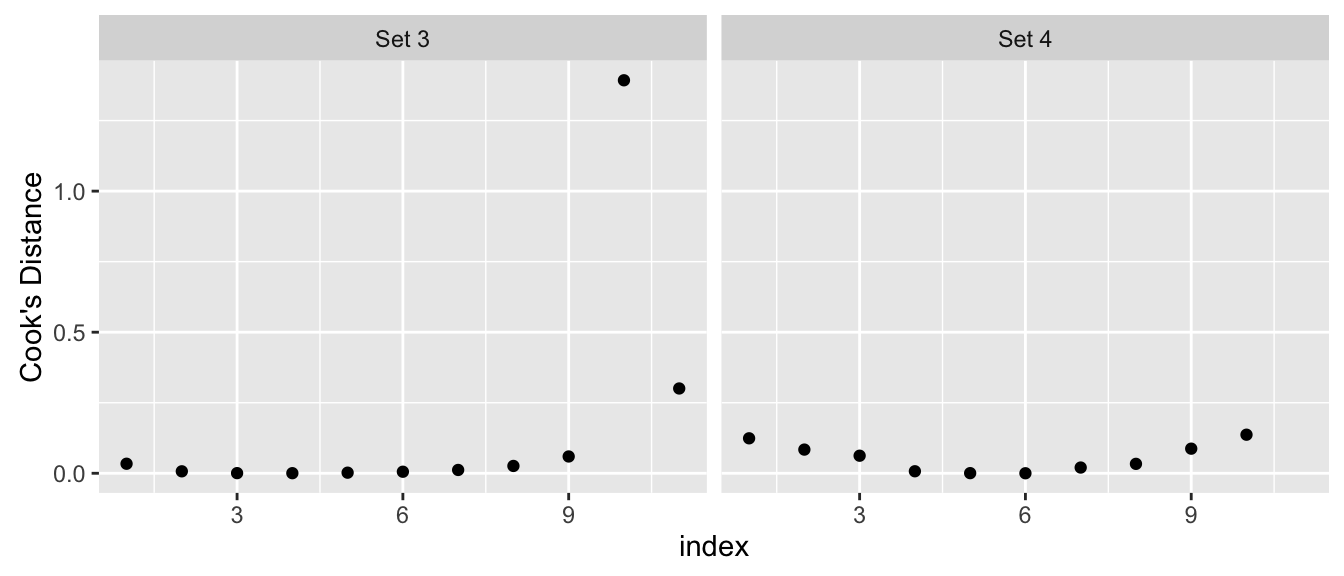
\includegraphics{Statistical_Methods_II_files/figure-latex/unnamed-chunk-72-1.pdf}

Using the \texttt{summary()} function, we can test hypotheses about if
the y-intercept or slope could be equal to zero, but we might be
interested in confidence intervals for the regression line at girth
values of 10 and 12.

\begin{Shaded}
\begin{Highlighting}[]
\CommentTok{# We could find the regression line heights and CI using }
\CommentTok{# either predict() or lsmeans()}
\KeywordTok{predict}\NormalTok{(model, }\DataTypeTok{newdata=}\KeywordTok{data.frame}\NormalTok{(}\DataTypeTok{Girth=}\KeywordTok{c}\NormalTok{(}\DecValTok{10}\NormalTok{,}\DecValTok{12}\NormalTok{)), }\DataTypeTok{interval=}\StringTok{'conf'} \NormalTok{)}
\end{Highlighting}
\end{Shaded}

\begin{verbatim}
##        fit      lwr      upr
## 1 13.71511 11.44781 15.98240
## 2 23.84682 22.16204 25.53159
\end{verbatim}

\begin{Shaded}
\begin{Highlighting}[]
\KeywordTok{lsmeans}\NormalTok{(model, }\DataTypeTok{specs =} \NormalTok{~Girth, }\DataTypeTok{at=}\KeywordTok{list}\NormalTok{(}\DataTypeTok{Girth=}\KeywordTok{c}\NormalTok{(}\DecValTok{10}\NormalTok{,}\DecValTok{12}\NormalTok{)) )  }
\end{Highlighting}
\end{Shaded}

\begin{verbatim}
##  Girth   lsmean        SE df lower.CL upper.CL
##     10 13.71511 1.1085761 29 11.44781 15.98240
##     12 23.84682 0.8237582 29 22.16204 25.53159
## 
## Confidence level used: 0.95
\end{verbatim}

The \texttt{lsmeans()} function requires us to specify the grid of
reference points we are interested as well as which variable or
variables we wish to separate out. In the simple regression case, the
\texttt{specs} argument is just the single covariate.

We might next ask if the difference in volume between a tree with 10
inch girth is statistically different than a tree with 12 inch girth? In
other words, we want to test
\[ H_0:\; (\beta_0 + \beta_1\cdot10 ) - (\beta_0 + \beta_1 \cdot 12) = 0\]
\[ H_a:\; (\beta_0 + \beta_1\cdot10 ) - (\beta_0 + \beta_1 \cdot 12) \ne 0\]

In this case, we want to look at all possible pairwise differences
between the predicted values at \(10\) and \(12\).

\begin{Shaded}
\begin{Highlighting}[]
\KeywordTok{lsmeans}\NormalTok{(model, }\DataTypeTok{specs =} \NormalTok{pairwise~Girth,}
        \DataTypeTok{at=}\KeywordTok{list}\NormalTok{(}\DataTypeTok{Girth=}\KeywordTok{c}\NormalTok{(}\DecValTok{10}\NormalTok{,}\DecValTok{12}\NormalTok{)) ) }
\end{Highlighting}
\end{Shaded}

\begin{verbatim}
## $lsmeans
##  Girth   lsmean        SE df lower.CL upper.CL
##     10 13.71511 1.1085761 29 11.44781 15.98240
##     12 23.84682 0.8237582 29 22.16204 25.53159
## 
## Confidence level used: 0.95 
## 
## $contrasts
##  contrast  estimate        SE df t.ratio p.value
##  10 - 12  -10.13171 0.4947539 29 -20.478  <.0001
\end{verbatim}

Notice that if I was interested in 3 points, we would get all of the
differences.

\begin{Shaded}
\begin{Highlighting}[]
\KeywordTok{lsmeans}\NormalTok{(model, }\DataTypeTok{specs =} \NormalTok{pairwise~Girth,}
        \DataTypeTok{at=}\KeywordTok{list}\NormalTok{(}\DataTypeTok{Girth=}\KeywordTok{c}\NormalTok{(}\DecValTok{10}\NormalTok{,}\DecValTok{11}\NormalTok{,}\DecValTok{12}\NormalTok{)) ) }
\end{Highlighting}
\end{Shaded}

\begin{verbatim}
## $lsmeans
##  Girth   lsmean        SE df lower.CL upper.CL
##     10 13.71511 1.1085761 29 11.44781 15.98240
##     11 18.78096 0.9447560 29 16.84872 20.71320
##     12 23.84682 0.8237582 29 22.16204 25.53159
## 
## Confidence level used: 0.95 
## 
## $contrasts
##  contrast   estimate        SE df t.ratio p.value
##  10 - 11   -5.065856 0.2473770 29 -20.478  <.0001
##  10 - 12  -10.131713 0.4947539 29 -20.478  <.0001
##  11 - 12   -5.065856 0.2473770 29 -20.478  <.0001
## 
## P value adjustment: tukey method for comparing a family of 3 estimates
\end{verbatim}

\subsection{1-way ANOVA}\label{way-anova-1}

To consider the pairwise contrasts between different levels we will
consider the college student hostility data again. A clinical
psychologist wished to compare three methods for reducing hostility
levels in university students, and used a certain test (HLT) to measure
the degree of hostility. A high score on the test indicated great
hostility. The psychologist used \(24\) students who obtained high and
nearly equal scores in the experiment. Eight subjects were selected at
random from among the \(24\) problem cases and were treated with method
1, seven of the remaining \(16\) students were selected at random and
treated with method 2 while the remaining nine students were treated
with method 3. All treatments were continued for a one-semester period.
Each student was given the HLT test at the end of the semester, with the
results show in the following table.

\begin{Shaded}
\begin{Highlighting}[]
\NormalTok{Hostility <-}\StringTok{ }\KeywordTok{data.frame}\NormalTok{(}
  \DataTypeTok{HLT =} \KeywordTok{c}\NormalTok{(}\DecValTok{96}\NormalTok{,}\DecValTok{79}\NormalTok{,}\DecValTok{91}\NormalTok{,}\DecValTok{85}\NormalTok{,}\DecValTok{83}\NormalTok{,}\DecValTok{91}\NormalTok{,}\DecValTok{82}\NormalTok{,}\DecValTok{87}\NormalTok{,}
          \DecValTok{77}\NormalTok{,}\DecValTok{76}\NormalTok{,}\DecValTok{74}\NormalTok{,}\DecValTok{73}\NormalTok{,}\DecValTok{78}\NormalTok{,}\DecValTok{71}\NormalTok{,}\DecValTok{80}\NormalTok{,}
          \DecValTok{66}\NormalTok{,}\DecValTok{73}\NormalTok{,}\DecValTok{69}\NormalTok{,}\DecValTok{66}\NormalTok{,}\DecValTok{77}\NormalTok{,}\DecValTok{73}\NormalTok{,}\DecValTok{71}\NormalTok{,}\DecValTok{70}\NormalTok{,}\DecValTok{74}\NormalTok{),}
  \DataTypeTok{Method =} \KeywordTok{c}\NormalTok{( }\KeywordTok{rep}\NormalTok{(}\StringTok{'M1'}\NormalTok{,}\DecValTok{8}\NormalTok{), }\KeywordTok{rep}\NormalTok{(}\StringTok{'M2'}\NormalTok{,}\DecValTok{7}\NormalTok{), }\KeywordTok{rep}\NormalTok{(}\StringTok{'M3'}\NormalTok{,}\DecValTok{9}\NormalTok{) ) )}
\end{Highlighting}
\end{Shaded}

\begin{Shaded}
\begin{Highlighting}[]
\KeywordTok{ggplot}\NormalTok{(Hostility, }\KeywordTok{aes}\NormalTok{(}\DataTypeTok{x=}\NormalTok{Method, }\DataTypeTok{y=}\NormalTok{HLT)) +}
\StringTok{  }\KeywordTok{geom_boxplot}\NormalTok{()}
\end{Highlighting}
\end{Shaded}

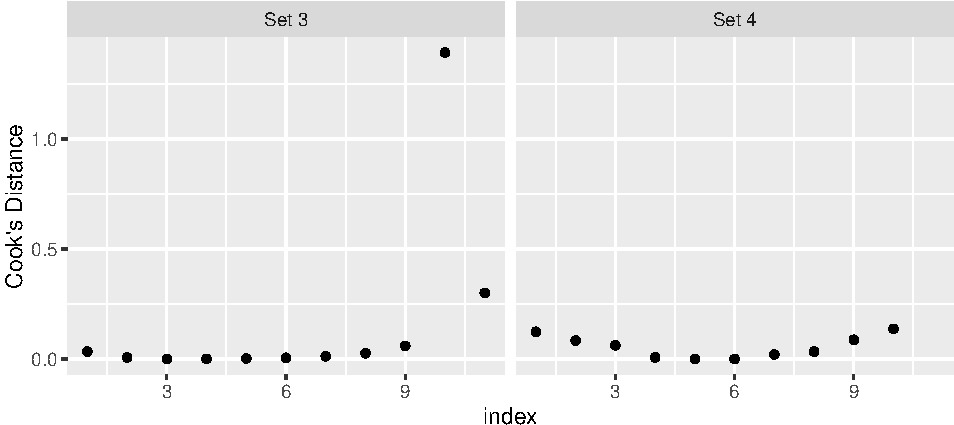
\includegraphics{Statistical_Methods_II_files/figure-latex/unnamed-chunk-77-1.pdf}

To use the \texttt{lsmeans()}, we again will use the pairwise command
where we specify that we want all the pairwise contrasts between Method
levels.

\begin{Shaded}
\begin{Highlighting}[]
\NormalTok{model <-}\StringTok{ }\KeywordTok{lm}\NormalTok{( HLT ~}\StringTok{ }\NormalTok{Method, }\DataTypeTok{data=}\NormalTok{Hostility )}
\KeywordTok{lsmeans}\NormalTok{(model, pairwise~Method)}
\end{Highlighting}
\end{Shaded}

\begin{verbatim}
## $lsmeans
##  Method   lsmean       SE df lower.CL upper.CL
##  M1     86.75000 1.518172 21 83.59279 89.90721
##  M2     75.57143 1.622994 21 72.19623 78.94663
##  M3     71.00000 1.431347 21 68.02335 73.97665
## 
## Confidence level used: 0.95 
## 
## $contrasts
##  contrast  estimate       SE df t.ratio p.value
##  M1 - M2  11.178571 2.222377 21   5.030  0.0002
##  M1 - M3  15.750000 2.086528 21   7.548  <.0001
##  M2 - M3   4.571429 2.163993 21   2.112  0.1114
## 
## P value adjustment: tukey method for comparing a family of 3 estimates
\end{verbatim}

\subsection{ANCOVA}\label{ancova}

We will return to the \texttt{ToothGrowth} dataset and calculate all the
interesting contrasts we previously built by hand.

\begin{Shaded}
\begin{Highlighting}[]
\KeywordTok{data}\NormalTok{(}\StringTok{'ToothGrowth'}\NormalTok{)}
\NormalTok{ToothGrowth$logDose <-}\StringTok{ }\KeywordTok{log}\NormalTok{( ToothGrowth$dose )}
\NormalTok{m <-}\StringTok{ }\KeywordTok{lm}\NormalTok{(len ~}\StringTok{ }\NormalTok{logDose *}\StringTok{ }\NormalTok{supp, }\DataTypeTok{data=}\NormalTok{ToothGrowth)}
\NormalTok{ToothGrowth <-}\StringTok{ }\KeywordTok{cbind}\NormalTok{(ToothGrowth, }\KeywordTok{predict}\NormalTok{(m, }\DataTypeTok{interval=}\StringTok{'conf'}\NormalTok{))}
\KeywordTok{ggplot}\NormalTok{(ToothGrowth, }\KeywordTok{aes}\NormalTok{(}\DataTypeTok{x=}\NormalTok{logDose, }\DataTypeTok{color=}\NormalTok{supp, }\DataTypeTok{fill=}\NormalTok{supp)) +}
\StringTok{  }\KeywordTok{geom_ribbon}\NormalTok{( }\KeywordTok{aes}\NormalTok{(}\DataTypeTok{ymin=}\NormalTok{lwr, }\DataTypeTok{ymax=}\NormalTok{upr), }\DataTypeTok{alpha=}\NormalTok{.}\DecValTok{3} \NormalTok{) +}
\StringTok{  }\KeywordTok{geom_line}\NormalTok{( }\KeywordTok{aes}\NormalTok{(}\DataTypeTok{y=}\NormalTok{fit) ) +}
\StringTok{  }\KeywordTok{geom_point}\NormalTok{( }\KeywordTok{aes}\NormalTok{(}\DataTypeTok{y=}\NormalTok{len) )}
\end{Highlighting}
\end{Shaded}

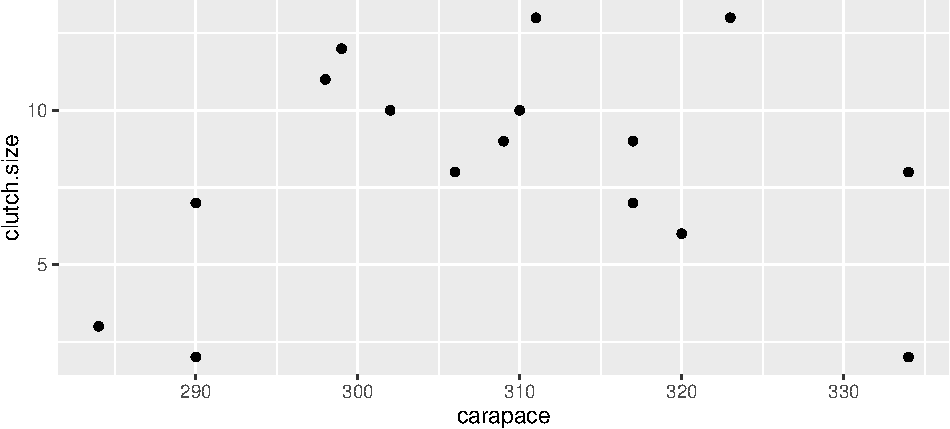
\includegraphics{Statistical_Methods_II_files/figure-latex/unnamed-chunk-79-1.pdf}

First, lets get the y-intercept for each group. In the following code,
the formula with the \texttt{\textbar{}\ supp} part says that we want to
do all the calculations for each level of the supplement types. The call
to \texttt{lsmeans()} calculates the response at logDose level 0. By
passing the result of the \texttt{lsmeans()} function call to the
\texttt{summary()} function, we can tell the summary function to print
out both the confidence intervals and t-tests.

\begin{Shaded}
\begin{Highlighting}[]
\KeywordTok{lsmeans}\NormalTok{(m, ~logDose |}\StringTok{ }\NormalTok{supp, }\DataTypeTok{at=}\KeywordTok{list}\NormalTok{(}\DataTypeTok{logDose=}\DecValTok{0}\NormalTok{)) %>%}\StringTok{ }
\StringTok{  }\KeywordTok{summary}\NormalTok{(}\DataTypeTok{infer=}\KeywordTok{c}\NormalTok{(}\OtherTok{TRUE}\NormalTok{,}\OtherTok{TRUE}\NormalTok{))}
\end{Highlighting}
\end{Shaded}

\begin{verbatim}
## supp = OJ:
##  logDose   lsmean        SE df lower.CL upper.CL t.ratio p.value
##        0 20.66333 0.6791481 56 19.30284 22.02383  30.425  <.0001
## 
## supp = VC:
##  logDose   lsmean        SE df lower.CL upper.CL t.ratio p.value
##        0 16.96333 0.6791481 56 15.60284 18.32383  24.977  <.0001
## 
## Confidence level used: 0.95
\end{verbatim}

Next we estimated the tooth growth for a guinea pig with a logdose =
-.69 (i.e.~dose=1/2) for both the OJ and VC supplements. We also wanted
to calculate the contrast between the two supplement predictions.

\begin{Shaded}
\begin{Highlighting}[]
\KeywordTok{lsmeans}\NormalTok{(m, pairwise~logDose*supp, }\DataTypeTok{at=}\KeywordTok{list}\NormalTok{(}\DataTypeTok{logDose=}\NormalTok{-.}\DecValTok{69}\NormalTok{)) %>%}\StringTok{ }
\StringTok{  }\KeywordTok{summary}\NormalTok{(}\DataTypeTok{infer=}\KeywordTok{c}\NormalTok{(}\OtherTok{TRUE}\NormalTok{,}\OtherTok{TRUE}\NormalTok{))}
\end{Highlighting}
\end{Shaded}

\begin{verbatim}
## $lsmeans
##  logDose supp   lsmean       SE df lower.CL upper.CL t.ratio p.value
##    -0.69 OJ   14.27746 1.070905 56 12.13218 16.42274  13.332  <.0001
##    -0.69 VC    7.92456 1.070905 56  5.77928 10.06984   7.400  <.0001
## 
## Confidence level used: 0.95 
## 
## $contrasts
##  contrast            estimate       SE df lower.CL upper.CL t.ratio
##  -0.69,OJ - -0.69,VC   6.3529 1.514488 56 3.319016 9.386784   4.195
##  p.value
##   0.0001
## 
## Confidence level used: 0.95
\end{verbatim}

We next make the same comparison for logdose = 0.69 (i.e.~dose=2).

\begin{Shaded}
\begin{Highlighting}[]
\KeywordTok{lsmeans}\NormalTok{(m, pairwise~logDose*supp, }\DataTypeTok{at=}\KeywordTok{list}\NormalTok{(}\DataTypeTok{logDose=}\NormalTok{.}\DecValTok{69}\NormalTok{)) %>%}\StringTok{ }
\StringTok{  }\KeywordTok{summary}\NormalTok{(}\DataTypeTok{infer=}\KeywordTok{c}\NormalTok{(}\OtherTok{TRUE}\NormalTok{,}\OtherTok{TRUE}\NormalTok{))}
\end{Highlighting}
\end{Shaded}

\begin{verbatim}
## $lsmeans
##  logDose supp   lsmean       SE df lower.CL upper.CL t.ratio p.value
##     0.69 OJ   27.04921 1.070905 56 24.90393 29.19449  25.258  <.0001
##     0.69 VC   26.00211 1.070905 56 23.85683 28.14739  24.281  <.0001
## 
## Confidence level used: 0.95 
## 
## $contrasts
##  contrast          estimate       SE df  lower.CL upper.CL t.ratio p.value
##  0.69,OJ - 0.69,VC   1.0471 1.514488 56 -1.986784 4.080984   0.691  0.4922
## 
## Confidence level used: 0.95
\end{verbatim}

While \texttt{lsmeans()} makes it very easy to calculate the \(\hat{y}\)
value for some covariate combination or some difference of \(\hat{y}\)
values, it doesn't handle slope parameters particularly well. The
companion function \texttt{lstrends()} is intended to make similar
calculations among slopes easy to create. We will now assess the
difference in slopes between the two groups.

\begin{Shaded}
\begin{Highlighting}[]
\KeywordTok{lstrends}\NormalTok{(m, ~logDose*supp, }\DataTypeTok{var =} \StringTok{'logDose'}\NormalTok{)}
\end{Highlighting}
\end{Shaded}

\begin{verbatim}
##  logDose supp logDose.trend       SE df  lower.CL upper.CL
##        0 OJ        9.254889 1.200009 56  6.850981 11.65880
##        0 VC       13.099671 1.200009 56 10.695763 15.50358
## 
## Confidence level used: 0.95
\end{verbatim}

\begin{Shaded}
\begin{Highlighting}[]
\KeywordTok{lstrends}\NormalTok{(m, pairwise~logDose*supp, }\DataTypeTok{var =} \StringTok{'logDose'}\NormalTok{)}
\end{Highlighting}
\end{Shaded}

\begin{verbatim}
## $lstrends
##  logDose supp logDose.trend       SE df  lower.CL upper.CL
##        0 OJ        9.254889 1.200009 56  6.850981 11.65880
##        0 VC       13.099671 1.200009 56 10.695763 15.50358
## 
## Confidence level used: 0.95 
## 
## $contrasts
##  contrast     estimate      SE df t.ratio p.value
##  0,OJ - 0,VC -3.844782 1.69707 56  -2.266  0.0274
\end{verbatim}

\subsubsection{\texorpdfstring{Common \texttt{lsmeans()}
mistake}{Common lsmeans() mistake}}\label{common-lsmeans-mistake}

It is very common to make a mistake using \texttt{lsmeans()} or
\texttt{lstrends()} if you don't understand what the specification
formula means. In particular what happens if you were to use
\texttt{\textasciitilde{}logDose} instead of the correct
\texttt{\textasciitilde{}logDose*supp}.

Consider the case where we are interested in making predictions for each
suppliment type at \(1/2\) dose (logDose=-0.69).

\begin{Shaded}
\begin{Highlighting}[]
\KeywordTok{lsmeans}\NormalTok{(m, ~logDose*supp, }\DataTypeTok{at=}\KeywordTok{list}\NormalTok{(}\DataTypeTok{logDose=}\NormalTok{-.}\DecValTok{69}\NormalTok{))}
\end{Highlighting}
\end{Shaded}

\begin{verbatim}
##  logDose supp   lsmean       SE df lower.CL upper.CL
##    -0.69 OJ   14.27746 1.070905 56 12.13218 16.42274
##    -0.69 VC    7.92456 1.070905 56  5.77928 10.06984
## 
## Confidence level used: 0.95
\end{verbatim}

If I were to accidently forget the \texttt{supp} part of this, then
\texttt{lsmeans()} would figure that I wanted to \emph{average} over the
two levels and give me the average of \(14.28\) and \(7.92\), which is
\(11.1\). With the interaction term in the model, it is unlikely that I
would want to do this, but \texttt{lsmeans()} complains a little but
lets me do it.

\begin{Shaded}
\begin{Highlighting}[]
\KeywordTok{lsmeans}\NormalTok{(m, ~logDose, }\DataTypeTok{at=}\KeywordTok{list}\NormalTok{(}\DataTypeTok{logDose=}\NormalTok{-.}\DecValTok{69}\NormalTok{))}
\end{Highlighting}
\end{Shaded}

\begin{verbatim}
## NOTE: Results may be misleading due to involvement in interactions
\end{verbatim}

\begin{verbatim}
##  logDose   lsmean       SE df lower.CL upper.CL
##    -0.69 11.10101 0.757244 56 9.584068 12.61795
## 
## Results are averaged over the levels of: supp 
## Confidence level used: 0.95
\end{verbatim}

What would happen if we only use \texttt{supp} in the formula
specification? In this case we are lucky because the
\texttt{logDose=-0.69} specified what dose level to look at. If we had
forgotten to specify this, then we would have done this calculation at
the mean \texttt{logDose} value, which happens to be zero.

\begin{Shaded}
\begin{Highlighting}[]
\KeywordTok{lsmeans}\NormalTok{(m, ~supp*logDose, }\DataTypeTok{at=}\KeywordTok{list}\NormalTok{(}\DataTypeTok{logDose=}\DecValTok{0}\NormalTok{))}
\end{Highlighting}
\end{Shaded}

\begin{verbatim}
##  supp logDose   lsmean        SE df lower.CL upper.CL
##  OJ         0 20.66333 0.6791481 56 19.30284 22.02383
##  VC         0 16.96333 0.6791481 56 15.60284 18.32383
## 
## Confidence level used: 0.95
\end{verbatim}

\begin{Shaded}
\begin{Highlighting}[]
\KeywordTok{lsmeans}\NormalTok{(m, ~supp)}
\end{Highlighting}
\end{Shaded}

\begin{verbatim}
## NOTE: Results may be misleading due to involvement in interactions
\end{verbatim}

\begin{verbatim}
##  supp   lsmean        SE df lower.CL upper.CL
##  OJ   20.66333 0.6791481 56 19.30284 22.02383
##  VC   16.96333 0.6791481 56 15.60284 18.32383
## 
## Confidence level used: 0.95
\end{verbatim}

Because the averaging over factor levels isn't what I typically want to
do, I start the analysis making sure the model formula I used in the
\texttt{lm()} command is the same as the one I pass into
\texttt{lsmeans()}.

\section{Exercises}\label{exercises-4}

\begin{enumerate}
\def\labelenumi{\arabic{enumi}.}
\item
  We will examine a dataset that summarizes cars featured in the
  magazine Motor Trend during the year 1974. In particular we will
  examine the relationship between the vehicles gas mileage
  (\texttt{mpg}) versus the weight (\texttt{wt}) and number of cylinders
  (\texttt{cyl}) of the vehicle.

\begin{Shaded}
\begin{Highlighting}[]
\KeywordTok{library}\NormalTok{(ggplot2)}
\KeywordTok{library}\NormalTok{(dplyr)}
\KeywordTok{data}\NormalTok{(mtcars)}
\NormalTok{mtcars$cyl <-}\StringTok{ }\KeywordTok{factor}\NormalTok{(mtcars$cyl)     }\CommentTok{# treat cylinders as categorical}
\KeywordTok{ggplot}\NormalTok{(mtcars, }\KeywordTok{aes}\NormalTok{(}\DataTypeTok{x=}\NormalTok{wt, }\DataTypeTok{col=}\NormalTok{cyl)) +}
\StringTok{  }\KeywordTok{geom_point}\NormalTok{(}\KeywordTok{aes}\NormalTok{(}\DataTypeTok{y=}\NormalTok{mpg, }\DataTypeTok{shape=}\NormalTok{cyl), }\DataTypeTok{size=}\DecValTok{4}\NormalTok{) +}
\StringTok{  }\KeywordTok{xlab}\NormalTok{(}\StringTok{'Weight (tons)'}\NormalTok{) +}
\StringTok{  }\KeywordTok{ylab}\NormalTok{(}\StringTok{'Miles per Gallon'}\NormalTok{) +}
\StringTok{  }\KeywordTok{labs}\NormalTok{(}\DataTypeTok{color=}\StringTok{'Cylinders'}\NormalTok{, }\DataTypeTok{shape=}\StringTok{'Cylinders'}\NormalTok{)}
\end{Highlighting}
\end{Shaded}

  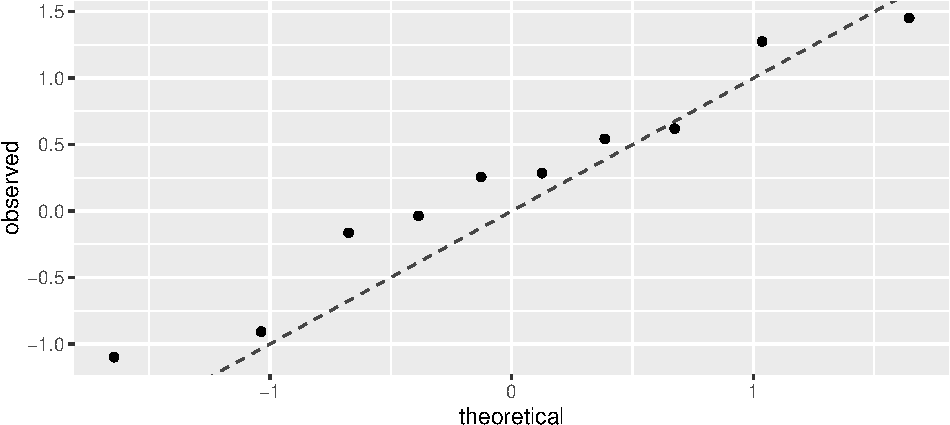
\includegraphics{Statistical_Methods_II_files/figure-latex/unnamed-chunk-87-1.pdf}

  \begin{enumerate}
  \def\labelenumii{\alph{enumii}.}
  \item
    Create a smaller set of data with just 9 observations (3 from each
    cylinder group) and create the design matrix \(\boldsymbol{X}\) for
    fitting the the model for estimating mpg using both weight and
    number of cylinders and their interaction using the following code:

\begin{Shaded}
\begin{Highlighting}[]
\NormalTok{mtcars.small <-}\StringTok{ }\NormalTok{mtcars %>%}\StringTok{      }
\StringTok{  }\KeywordTok{group_by}\NormalTok{(cyl) %>%}\StringTok{             }\CommentTok{# For each cylinder group}
\StringTok{  }\KeywordTok{arrange}\NormalTok{(cyl, wt) %>%}\StringTok{          }\CommentTok{# Reorder my dataset}
\StringTok{  }\KeywordTok{slice}\NormalTok{(}\DecValTok{1}\NormalTok{:}\DecValTok{3}\NormalTok{)                    }\CommentTok{# grab first three rows of each group}
\KeywordTok{model.matrix}\NormalTok{(  }\KeywordTok{lm}\NormalTok{(mpg ~}\StringTok{ }\NormalTok{wt*cyl, }\DataTypeTok{data=}\NormalTok{mtcars.small) )}
\end{Highlighting}
\end{Shaded}

\begin{verbatim}
##   (Intercept)    wt cyl6 cyl8 wt:cyl6 wt:cyl8
## 1           1 1.513    0    0   0.000   0.000
## 2           1 1.615    0    0   0.000   0.000
## 3           1 1.835    0    0   0.000   0.000
## 4           1 2.620    1    0   2.620   0.000
## 5           1 2.770    1    0   2.770   0.000
## 6           1 2.875    1    0   2.875   0.000
## 7           1 3.170    0    1   0.000   3.170
## 8           1 3.435    0    1   0.000   3.435
## 9           1 3.440    0    1   0.000   3.440
## attr(,"assign")
## [1] 0 1 2 2 3 3
## attr(,"contrasts")
## attr(,"contrasts")$cyl
## [1] "contr.treatment"
\end{verbatim}

    \emph{Hint: the purpose of this step is to make sure everyone knows
    the column order of the design matrix so that you interprete the
    \(\beta\) terms in the correct order.}
  \item
    Denote the coefficients obtained from the summary of your
    \texttt{lm()} call as \(\hat{\beta}_{0}\) to \(\hat{\beta}_{5}\) (in
    the order given by R). Write your interaction model out using
    subscript notation and should be in the form \[y_{i}=\begin{cases}
    ??????? & \;\;\textrm{if 4 cylinder}\\
    ??????? & \;\;\textrm{if 6 cylinder}\\
    ??????? & \;\;\textrm{if 8 cylinder}
    \end{cases}\] and give an interpretation for each \(\beta_{j}\)
    value.

    \begin{enumerate}
    \def\labelenumiii{\roman{enumiii}.}
    \tightlist
    \item
      \(\hat{\beta}_0\) = ???
    \item
      \(\hat{\beta}_1\) = ???
    \item
      \(\hat{\beta}_2\) = ???
    \item
      \(\hat{\beta}_3\) = ???
    \item
      \(\hat{\beta}_4\) = ???
    \item
      \(\hat{\beta}_5\) = ???
    \end{enumerate}
  \item
    Using the full dataset, fit the model that predicts mpg using both
    weight and number of cylinders and their interaction using the
    command

\begin{Shaded}
\begin{Highlighting}[]
\NormalTok{model <-}\StringTok{ }\KeywordTok{lm}\NormalTok{(mpg ~}\StringTok{ }\NormalTok{wt*cyl, }\DataTypeTok{data=}\NormalTok{mtcars)}
\end{Highlighting}
\end{Shaded}

    Create a vector of fitted values, add it to the data frame
    \texttt{mtcars} and then create a plot that includes the regression
    lines.
  \item
    What is the estimated mpg of a 6-cylinder vehicle weighing 3.5 tons?
    What is the estimated mpg of a 8-cylinder vehicle weight 3.5 tons?
    Give the associated 95\% confidence intervals. Calculate these using
    the \texttt{predict()} function. \emph{Warning: When making the new
    data frame, make sure that R interprets cyl as a factor by either
    coercing it to a factor after creation or inputing the cylinder as a
    string (i.e.~as ``6'' instead of 6).}
  \item
    Recalculate your answer to part (d) using the \texttt{glht()}
    function. Also give the estimate and confidence interval for the
    difference in mpg betwen the 8 and 6 cylinder vehicles that weight
    3.5 tones? Is there a statistically significant difference in mpg at
    3.5 tons?
  \item
    Recalculate your answer to part (e) using the \texttt{lsmeans()}
    function.
  \item
    Are the slopes of the 8-cylinder and 6-cylinder vehicles
    statistically different? Use \texttt{glht()} to produce this result.
  \item
    Recalculate your answer to part (g) using the \texttt{lstrends()}
    function.
  \end{enumerate}
\end{enumerate}

\chapter{Diagnostics and
Transformations}\label{diagnostics-and-transformations}

We will be interested in analyzing whether or not our linear model is a
good model and whether or not the data violate any of the assumptions
that are required. In general we will be interested in three classes of
assumption violations and our diagnostic measures might be able detect
one or more of the following issues:

\begin{enumerate}
\def\labelenumi{\arabic{enumi}.}
\item
  Unusual observations that contribute too much influence to the
  analysis. These few observations might drastically change the outcome
  of the model.
\item
  Model misspecification. Our assumption that
  \(E\left[\boldsymbol{y}\right]=\boldsymbol{X}\boldsymbol{\beta}\)
  might be wrong and we might need to include different covariates in
  the model to get a satisfactory result.
\item
  Error distribution. We have assumed that
  \(\boldsymbol{\epsilon}\sim MVN\left(\boldsymbol{0},\sigma^{2}\boldsymbol{I}\right)\)
  but autocorrelation, heteroscedasticity, and non-normality might be
  present.
\end{enumerate}

Often problems with one of these can be corrected by tranforming either
the explanatory or response variables.

\section{Detecting Assumption
Violations}\label{detecting-assumption-violations}

Throughout this chapter I will use data created by Francis Anscombe that
show how simple linear regression can be misused. In particular, these
data sets will show how our diagnostic measures will detect various
departures from the model assumptions.

The data are available in R as a data frame \texttt{anscombe} and is
loaded by default. The data consists of four datasets, each having the
same linear regression \(\hat{y}=3+0.5\,x\) but the data are drastically
different.

\begin{Shaded}
\begin{Highlighting}[]
\KeywordTok{library}\NormalTok{(ggplot2)}
\KeywordTok{library}\NormalTok{(dplyr)}

\CommentTok{# The anscombe dataset has 8 columns - x1,x2,x3,x4,y1,y2,y3,y4}
\CommentTok{# and I want it to have 3 columns - Set, X, Y}
\NormalTok{Anscombe <-}\StringTok{ }\KeywordTok{rbind}\NormalTok{( }
  \KeywordTok{data.frame}\NormalTok{(}\DataTypeTok{x=}\NormalTok{anscombe$x1, }\DataTypeTok{y=}\NormalTok{anscombe$y1, }\DataTypeTok{set=}\StringTok{'Set 1'}\NormalTok{),}
  \KeywordTok{data.frame}\NormalTok{(}\DataTypeTok{x=}\NormalTok{anscombe$x2, }\DataTypeTok{y=}\NormalTok{anscombe$y2, }\DataTypeTok{set=}\StringTok{'Set 2'}\NormalTok{),}
  \KeywordTok{data.frame}\NormalTok{(}\DataTypeTok{x=}\NormalTok{anscombe$x3, }\DataTypeTok{y=}\NormalTok{anscombe$y3, }\DataTypeTok{set=}\StringTok{'Set 3'}\NormalTok{),}
  \KeywordTok{data.frame}\NormalTok{(}\DataTypeTok{x=}\NormalTok{anscombe$x4, }\DataTypeTok{y=}\NormalTok{anscombe$y4, }\DataTypeTok{set=}\StringTok{'Set 4'}\NormalTok{)) }

\CommentTok{# order them by their x values, and add an index column}
\NormalTok{Anscombe <-}\StringTok{ }\NormalTok{Anscombe %>%}\StringTok{ }
\StringTok{  }\KeywordTok{group_by}\NormalTok{(set) %>%}\StringTok{       }\CommentTok{# Every subsequent action happens by dataset}
\StringTok{  }\KeywordTok{arrange}\NormalTok{(x,y) %>%}\StringTok{        }\CommentTok{# sort them on the x-values and if tied, by y-value}
\StringTok{  }\KeywordTok{mutate}\NormalTok{( }\DataTypeTok{index =} \DecValTok{1}\NormalTok{:}\KeywordTok{n}\NormalTok{() ) }\CommentTok{# give each observation within a set, an ID number}

\CommentTok{# Make a nice graph}
\KeywordTok{ggplot}\NormalTok{(Anscombe, }\KeywordTok{aes}\NormalTok{(}\DataTypeTok{x=}\NormalTok{x, }\DataTypeTok{y=}\NormalTok{y)) +}
\StringTok{ }\KeywordTok{geom_point}\NormalTok{() +}
\StringTok{ }\KeywordTok{facet_wrap}\NormalTok{(~set, }\DataTypeTok{scales=}\StringTok{'free'}\NormalTok{) +}
\StringTok{ }\KeywordTok{stat_smooth}\NormalTok{(}\DataTypeTok{method=}\StringTok{"lm"}\NormalTok{, }\DataTypeTok{formula=}\NormalTok{y~x, }\DataTypeTok{se=}\OtherTok{FALSE}\NormalTok{)}
\end{Highlighting}
\end{Shaded}

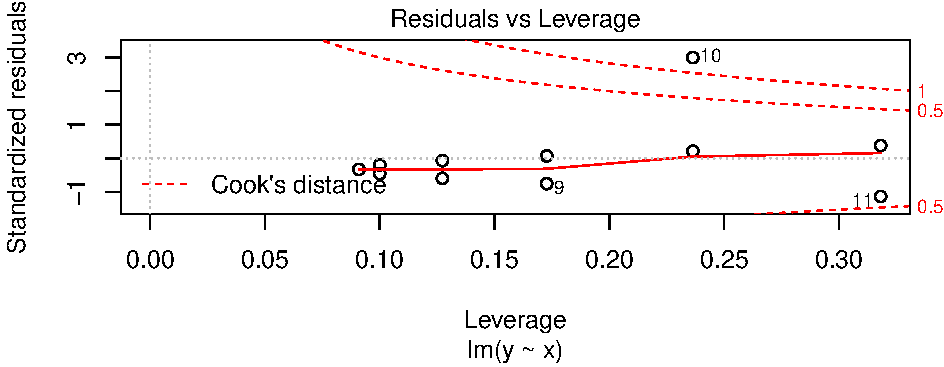
\includegraphics{Statistical_Methods_II_files/figure-latex/unnamed-chunk-91-1.pdf}

\subsection{Measures of Influence}\label{measures-of-influence}

\subsubsection{Standardized Residuals (aka Studentized
)}\label{standardized-residuals-aka-studentized}

Recall that we have

\[\begin{aligned}\hat{\boldsymbol{y}}   
  &=    \boldsymbol{X}\hat{\boldsymbol{\beta}}\\
    &=  \boldsymbol{X}\left(\boldsymbol{X}^{T}\boldsymbol{X}\right)^{-1}\boldsymbol{X}^{T}\boldsymbol{y}\\
    &=  \boldsymbol{H}\boldsymbol{y}\\
\end{aligned}\]

where the ``Hat Matrix'' is
\(\boldsymbol{H}=\boldsymbol{X}\left(\boldsymbol{X}^{T}\boldsymbol{X}\right)^{-1}\boldsymbol{X}^{T}\)
because we have \(\hat{\boldsymbol{y}}=\boldsymbol{H}\boldsymbol{y}\).
The elements of \(\boldsymbol{H}\) can be quite useful in diagnostics.
It can be shown that the variance of the \(i\)the residual is
\[Var\left(\hat{\epsilon}_{i}\right)=\sigma^{2}\left(1-\boldsymbol{H}_{ii}\right)\]
where \(\boldsymbol{H}_{ii}\) is the \(i\)th element of the main
diagonal of \(\boldsymbol{H}\). This suggests that I could rescale my
residuals to
\[\hat{\epsilon}_{i}^{*}=\frac{\hat{\epsilon}_{i}}{\hat{\sigma}\sqrt{1-\boldsymbol{H}_{ii}}}\]
which, if the normality and homoscedasticity assumptions hold, should
behave as a \(N\left(0,1\right)\) sample.

These rescaled residuals are called ``studentized residuals'', though R
typically refers to them as ``standardized''. Since we have a good
intuition about the scale of a standard normal distribution, the scale
of standardized residuals will give a good indicator if normality is
violated.

There are actually two types of studentized residuals, typically called
\emph{internal} and \emph{external} among statisticians. The version
presented above is the \emph{internal} version which can be obtained
using the R function \texttt{rstandard()} while the \emph{external}
version is available using \texttt{rstudent()}. Whenever you see R
present standardized residuals, they are talking about internally
studentized residuals. For sake of clarity, I will use the term
\emph{standardized} as well.

\paragraph{Example - Anscombe's set 3}\label{example---anscombes-set-3}

For the third dataset, the outlier is the ninth observation with
\(x_{9}=13\) and \(y_{9}=12.74\). We calculate the standardized
residuals using the function \texttt{rstandard()} and plot them

\begin{Shaded}
\begin{Highlighting}[]
\NormalTok{Set3 <-}\StringTok{ }\NormalTok{Anscombe %>%}\StringTok{ }\KeywordTok{filter}\NormalTok{(set ==}\StringTok{ 'Set 3'}\NormalTok{) }\CommentTok{# Just set 3}
\NormalTok{model <-}\StringTok{ }\KeywordTok{lm}\NormalTok{(y ~}\StringTok{ }\NormalTok{x, }\DataTypeTok{data=}\NormalTok{Set3)               }\CommentTok{# Fit the regression line}
\NormalTok{Set3$stdresid <-}\StringTok{ }\KeywordTok{rstandard}\NormalTok{(model)           }\CommentTok{# rstandard() returns the standardized residuals}

\KeywordTok{ggplot}\NormalTok{(Set3, }\KeywordTok{aes}\NormalTok{(}\DataTypeTok{x=}\NormalTok{index, }\DataTypeTok{y=}\NormalTok{stdresid)) +}\StringTok{    }\CommentTok{# make a plot}
\StringTok{  }\KeywordTok{geom_point}\NormalTok{() +}
\StringTok{  }\KeywordTok{labs}\NormalTok{(}\DataTypeTok{x=}\StringTok{'Observation Index'}\NormalTok{, }
       \DataTypeTok{y=}\StringTok{'Standardized Residuals'}\NormalTok{, }
       \DataTypeTok{title=}\StringTok{'Standardized Residuals vs Observation Index'}\NormalTok{)}
\end{Highlighting}
\end{Shaded}

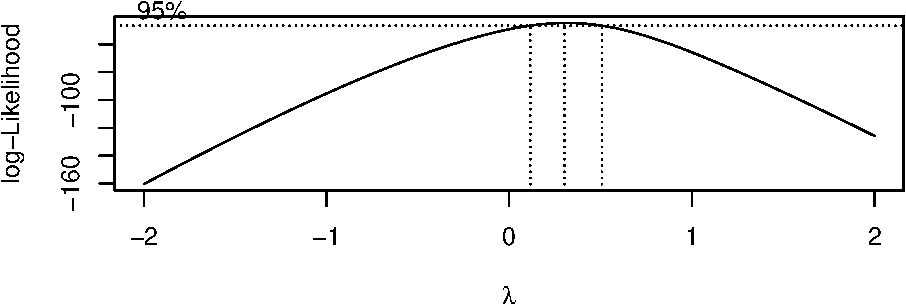
\includegraphics{Statistical_Methods_II_files/figure-latex/unnamed-chunk-92-1.pdf}

and we notice that the outlier residual is really big. If the model
assumptions were true, then the standardized residuals should follow a
standard normal distribution, and I would need to have hundreds of
observations before I wouldn't be surprised to see a residual more than
3 standard deviations from 0.

\subsubsection{Leverage}\label{leverage}

The extremely large standardized residual suggests that this data point
is important, but we would like to quantify how important this
observation actually is.

One way to quantify this is to look at the elements of
\(\boldsymbol{H}\). Because
\[\hat{y}_{i}=\sum_{j=1}^{n}\boldsymbol{H}_{ij}y_{j}\] then the \(i\)th
row of \(\boldsymbol{H}\) is a vector of weights that tell us how
influential a point \(y_{j}\) is for calculating the predicted value
\(\hat{y}_{i}\). If I look at just the main diagonal of
\(\boldsymbol{H}\), these are how much weight a point has on its
predicted value. As such, I can think of the \(\boldsymbol{H}_{ii}\) as
the amount of leverage a particular data point has on the regression
line.

Fortunately there is already a function \texttt{hatvalues()} to compute
these \(\boldsymbol{H}_{ii}\) values for me. We will compare the
leverages from Anscombe's set 3 versus set 4.

\begin{Shaded}
\begin{Highlighting}[]
\NormalTok{Set3 <-}\StringTok{ }\NormalTok{Anscombe %>%}\StringTok{ }\KeywordTok{filter}\NormalTok{( set ==}\StringTok{ 'Set 3'}\NormalTok{)}
\NormalTok{Set4 <-}\StringTok{ }\NormalTok{Anscombe %>%}\StringTok{ }\KeywordTok{filter}\NormalTok{( set ==}\StringTok{ 'Set 4'}\NormalTok{)}

\NormalTok{model3 <-}\StringTok{ }\KeywordTok{lm}\NormalTok{(y ~}\StringTok{ }\NormalTok{x, }\DataTypeTok{data =} \NormalTok{Set3 )}
\NormalTok{model4 <-}\StringTok{ }\KeywordTok{lm}\NormalTok{(y ~}\StringTok{ }\NormalTok{x, }\DataTypeTok{data =} \NormalTok{Set4 )}

\NormalTok{Set3 <-}\StringTok{ }\NormalTok{Set3 %>%}\StringTok{ }\KeywordTok{mutate}\NormalTok{(}\DataTypeTok{leverage =} \KeywordTok{hatvalues}\NormalTok{(model3))  }\CommentTok{# add leverage columns}
\NormalTok{Set4 <-}\StringTok{ }\NormalTok{Set4 %>%}\StringTok{ }\KeywordTok{mutate}\NormalTok{(}\DataTypeTok{leverage =} \KeywordTok{hatvalues}\NormalTok{(model4))}

\KeywordTok{ggplot}\NormalTok{( }\KeywordTok{rbind}\NormalTok{(Set3,Set4), }\KeywordTok{aes}\NormalTok{(}\DataTypeTok{x=}\NormalTok{index, }\DataTypeTok{y=}\NormalTok{leverage) ) +}
\StringTok{  }\KeywordTok{geom_point}\NormalTok{() +}
\StringTok{  }\KeywordTok{facet_grid}\NormalTok{( . ~}\StringTok{ }\NormalTok{set )}
\end{Highlighting}
\end{Shaded}

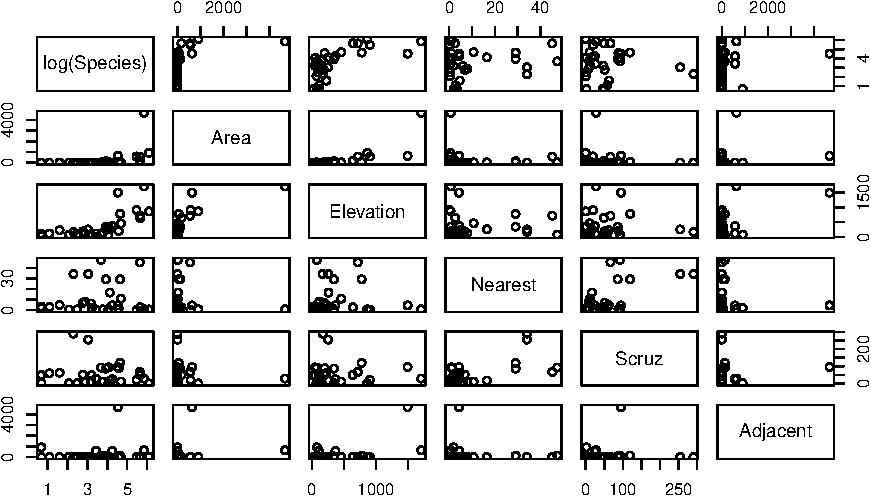
\includegraphics{Statistical_Methods_II_files/figure-latex/unnamed-chunk-93-1.pdf}

This leverage idea only picks out the \emph{potential} for a specific
value of \(x\) to be influential, but does not actually measure
influence. It has picked out the issue with the fourth data set, but
does not adequately address the outlier in set 3.

\subsubsection{Cook's Distance}\label{cooks-distance}

To attempt to measure the actual influence of an observation
\(\left\{ y_{i},\boldsymbol{x}_{i}^{T}\right\}\) on the linear model, we
consider the effect on the regression if we removed the observation and
fit the same model. Let
\[\hat{\boldsymbol{y}}=\boldsymbol{X}\hat{\boldsymbol{\beta}}\] be the
vector of predicted values, where \(\hat{\boldsymbol{\beta}}\) is
created using all of the data, and
\(\hat{\boldsymbol{y}}_{(i)}=\boldsymbol{X}\hat{\boldsymbol{\beta}}_{(i)}\)
be the vector of predicted values where
\(\hat{\boldsymbol{\beta}}_{(i)}\) was estimated using all of the data
except the \(i\)th observation. Letting \(p\) be the number of
\(\beta_{j}\) parameters as usual we define Cook's distance of the
\(i\)th observation as
\[ D_{i} = \frac{\left(\hat{\boldsymbol{y}}-\hat{\boldsymbol{y}}_{(i)}\right)^{T}\left(\hat{\boldsymbol{y}}-\hat{\boldsymbol{y}}_{(i)}\right)}{p\hat{\sigma}^{2}}\]
which boils down to saying if the predicted values have large changes
when the \(i\)th element is removed, then the distance is big. It can be
shown that this formula can be simplified to
\[D_{i}=\frac{\hat{\epsilon}_{i}^{*}\boldsymbol{H}_{ii}}{p\left(1-H_{ii}\right)}\]
which expresses Cook's distance in terms of the \(i\)th studentized
residual and the \(i\)th leverage.

Nicely, the R function \texttt{cooks.distance()} will calculate Cook's
distance.

\begin{Shaded}
\begin{Highlighting}[]
\NormalTok{Set3 <-}\StringTok{ }\NormalTok{Set3 %>%}\StringTok{ }\KeywordTok{mutate}\NormalTok{(}\DataTypeTok{cooksd =} \KeywordTok{cooks.distance}\NormalTok{(model3))  }
\NormalTok{Set4 <-}\StringTok{ }\NormalTok{Set4 %>%}\StringTok{ }\KeywordTok{mutate}\NormalTok{(}\DataTypeTok{cooksd =} \KeywordTok{cooks.distance}\NormalTok{(model4))}

\CommentTok{# Note: The high leverage point in set 4 has a Cook's distance of Infinity.}
\KeywordTok{ggplot}\NormalTok{(}\KeywordTok{rbind}\NormalTok{(Set3,Set4), }\KeywordTok{aes}\NormalTok{(}\DataTypeTok{x=}\NormalTok{index, }\DataTypeTok{y=}\NormalTok{cooksd)) +}\StringTok{ }
\StringTok{  }\KeywordTok{geom_point}\NormalTok{() +}
\StringTok{  }\KeywordTok{facet_grid}\NormalTok{(. ~}\StringTok{ }\NormalTok{set) +}
\StringTok{  }\KeywordTok{labs}\NormalTok{(}\DataTypeTok{y=}\StringTok{"Cook's Distance"}\NormalTok{)}
\end{Highlighting}
\end{Shaded}

\begin{verbatim}
## Warning: Removed 1 rows containing missing values (geom_point).
\end{verbatim}

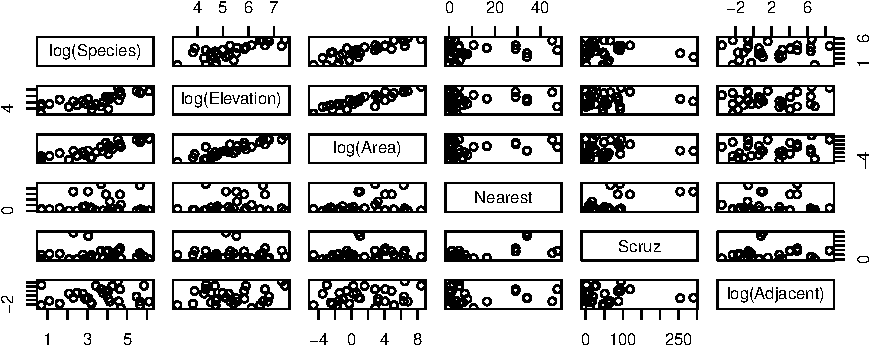
\includegraphics{Statistical_Methods_II_files/figure-latex/unnamed-chunk-94-1.pdf}

Some texts will give a rule of thumb that points with Cook's distances
greater than 1 should be considered influential, while other books claim
a reasonable rule of thumb is \(4/\left(n-p-1\right)\) where \(n\) is
the sample size, and \(p\) is the number of parameters in
\(\boldsymbol{\beta}\). My take on this, is that you should look for
values that are highly different from the rest of your data.

\subsection{Diagnostic Plots}\label{diagnostic-plots}

After fitting a linear model in R, you have the option of looking at
diagnostic plots that help to decide if any assumptions are being
violated. We will step through each of the plots that are generated by
the function \texttt{plot(model)} or using \texttt{ggplot2} using the
package \texttt{ggfortify}.

In the package \texttt{ggfortify} there is a function that will
calculate the diagnostics measures and add them to your dataset. This
will simplify our graphing process.

\begin{Shaded}
\begin{Highlighting}[]
\NormalTok{Set1 <-}\StringTok{ }\NormalTok{Anscombe %>%}\StringTok{ }\KeywordTok{filter}\NormalTok{(set ==}\StringTok{ 'Set 1'}\NormalTok{)}
\NormalTok{model <-}\StringTok{ }\KeywordTok{lm}\NormalTok{( y ~}\StringTok{ }\NormalTok{x, }\DataTypeTok{data=}\NormalTok{Set1)}
\NormalTok{Set1 <-}\StringTok{ }\KeywordTok{fortify}\NormalTok{(model)  }\CommentTok{# add dignostic measures to the dataset}
\NormalTok{Set1 %>%}\StringTok{ }\KeywordTok{round}\NormalTok{(}\DataTypeTok{digits=}\DecValTok{3}\NormalTok{) }\CommentTok{# show the dataset nicely}
\end{Highlighting}
\end{Shaded}

\begin{verbatim}
##        y  x  .hat .sigma .cooksd .fitted .resid .stdresid
## 1   4.26  4 0.318  1.273   0.123   5.000 -0.740    -0.725
## 2   5.68  5 0.236  1.310   0.004   5.501  0.179     0.166
## 3   7.24  6 0.173  1.220   0.127   6.001  1.239     1.102
## 4   4.82  7 0.127  1.147   0.154   6.501 -1.681    -1.455
## 5   6.95  8 0.100  1.311   0.000   7.001 -0.051    -0.043
## 6   8.81  9 0.091  1.218   0.062   7.501  1.309     1.110
## 7   8.04 10 0.100  1.312   0.000   8.001  0.039     0.033
## 8   8.33 11 0.127  1.310   0.002   8.501 -0.171    -0.148
## 9  10.84 12 0.173  1.100   0.279   9.001  1.839     1.635
## 10  7.58 13 0.236  1.056   0.489   9.501 -1.921    -1.778
## 11  9.96 14 0.318  1.311   0.000  10.001 -0.041    -0.041
\end{verbatim}

\subsubsection{Residuals vs Fitted}\label{residuals-vs-fitted}

In the simple linear regression the most useful plot to look at was the
residuals versus the \(x\)-covariate, but we also saw that this was
similar to looking at the residuals versus the fitted values. In the
general linear model, we will look at the residuals versus the fitted
values or possibly the studentized residuals versus the fitted values.

\paragraph{Polynomial relationships}\label{polynomial-relationships}

To explore how this plot can detect non-linear relationships between
\(y\) and \(x\), we will examine a data set from Ashton et al. (2007)
that relates the length of a tortoise's carapace to the number of eggs
laid in a clutch. The data are

\begin{Shaded}
\begin{Highlighting}[]
\NormalTok{Eggs <-}\StringTok{ }\KeywordTok{data.frame}\NormalTok{(}
  \DataTypeTok{carapace    =} \KeywordTok{c}\NormalTok{(}\DecValTok{284}\NormalTok{,}\DecValTok{290}\NormalTok{,}\DecValTok{290}\NormalTok{,}\DecValTok{290}\NormalTok{,}\DecValTok{298}\NormalTok{,}\DecValTok{299}\NormalTok{,}\DecValTok{302}\NormalTok{,}\DecValTok{306}\NormalTok{,}\DecValTok{306}\NormalTok{,}
                  \DecValTok{309}\NormalTok{,}\DecValTok{310}\NormalTok{,}\DecValTok{311}\NormalTok{,}\DecValTok{317}\NormalTok{,}\DecValTok{317}\NormalTok{,}\DecValTok{320}\NormalTok{,}\DecValTok{323}\NormalTok{,}\DecValTok{334}\NormalTok{,}\DecValTok{334}\NormalTok{),}
  \DataTypeTok{clutch.size =} \KeywordTok{c}\NormalTok{(}\DecValTok{3}\NormalTok{,}\DecValTok{2}\NormalTok{,}\DecValTok{7}\NormalTok{,}\DecValTok{7}\NormalTok{,}\DecValTok{11}\NormalTok{,}\DecValTok{12}\NormalTok{,}\DecValTok{10}\NormalTok{,}\DecValTok{8}\NormalTok{,}\DecValTok{8}\NormalTok{,}
                  \DecValTok{9}\NormalTok{,}\DecValTok{10}\NormalTok{,}\DecValTok{13}\NormalTok{,}\DecValTok{7}\NormalTok{,}\DecValTok{9}\NormalTok{,}\DecValTok{6}\NormalTok{,}\DecValTok{13}\NormalTok{,}\DecValTok{2}\NormalTok{,}\DecValTok{8}\NormalTok{)) }
\KeywordTok{ggplot}\NormalTok{(Eggs, }\KeywordTok{aes}\NormalTok{(}\DataTypeTok{x=}\NormalTok{carapace, }\DataTypeTok{y=}\NormalTok{clutch.size)) +}\StringTok{ }
\StringTok{  }\KeywordTok{geom_point}\NormalTok{()}
\end{Highlighting}
\end{Shaded}

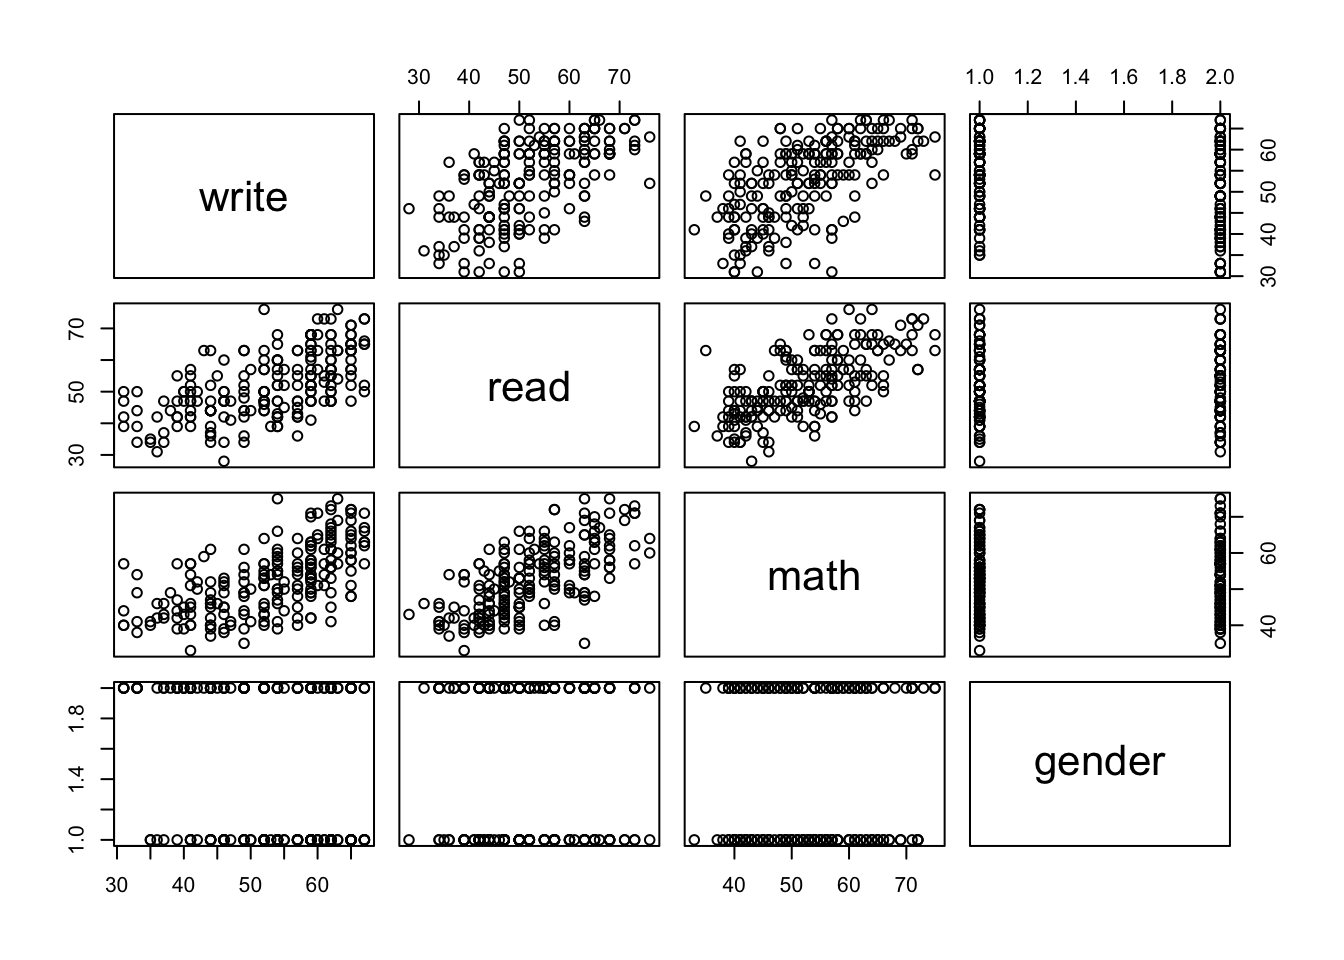
\includegraphics{Statistical_Methods_II_files/figure-latex/unnamed-chunk-96-1.pdf}

Looking at the data, it seems that we are violating the assumption that
a linear model is appropriate, but we will fit the model anyway and look
at the residual graph.

\begin{Shaded}
\begin{Highlighting}[]
\NormalTok{model <-}\StringTok{ }\KeywordTok{lm}\NormalTok{( clutch.size ~}\StringTok{ }\NormalTok{carapace, }\DataTypeTok{data=}\NormalTok{Eggs )}
\KeywordTok{plot}\NormalTok{(model, }\DataTypeTok{which=}\DecValTok{1}\NormalTok{)      }\CommentTok{# which=1 tells R to only make the first plot}
\end{Highlighting}
\end{Shaded}

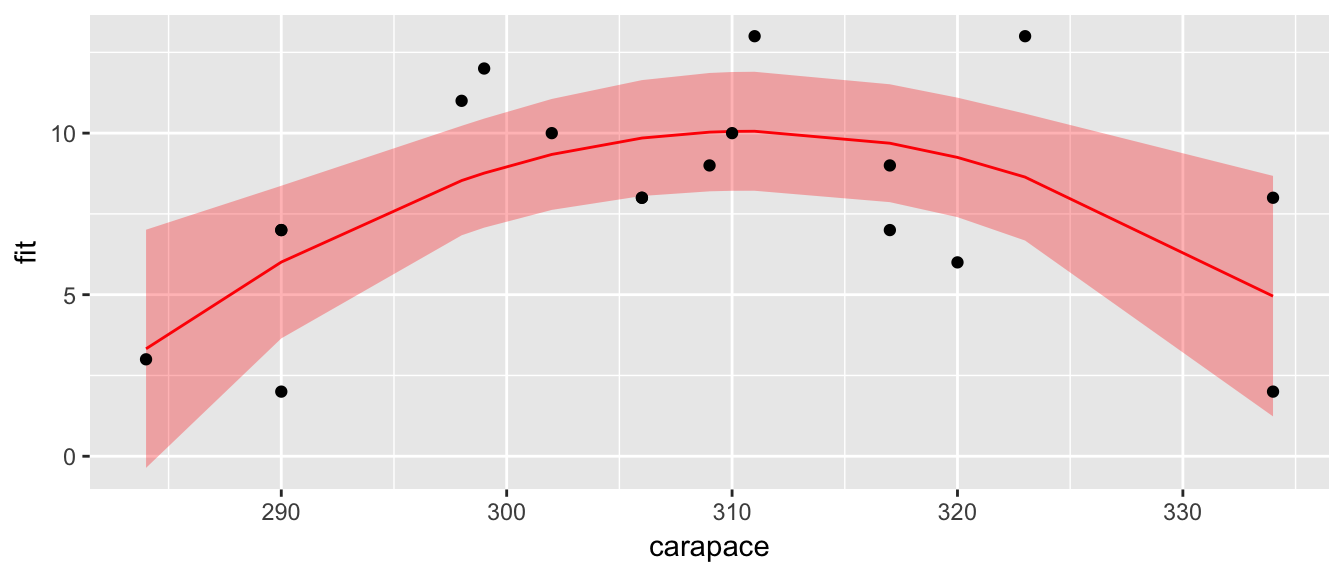
\includegraphics{Statistical_Methods_II_files/figure-latex/unnamed-chunk-97-1.pdf}

\begin{Shaded}
\begin{Highlighting}[]
\KeywordTok{library}\NormalTok{(ggfortify)        }\CommentTok{# need the ggfortify library for autoplot.lm() to work}
\KeywordTok{autoplot}\NormalTok{(model, }\DataTypeTok{which=}\DecValTok{1}\NormalTok{)  }\CommentTok{# same plot using ggplot2}
\end{Highlighting}
\end{Shaded}

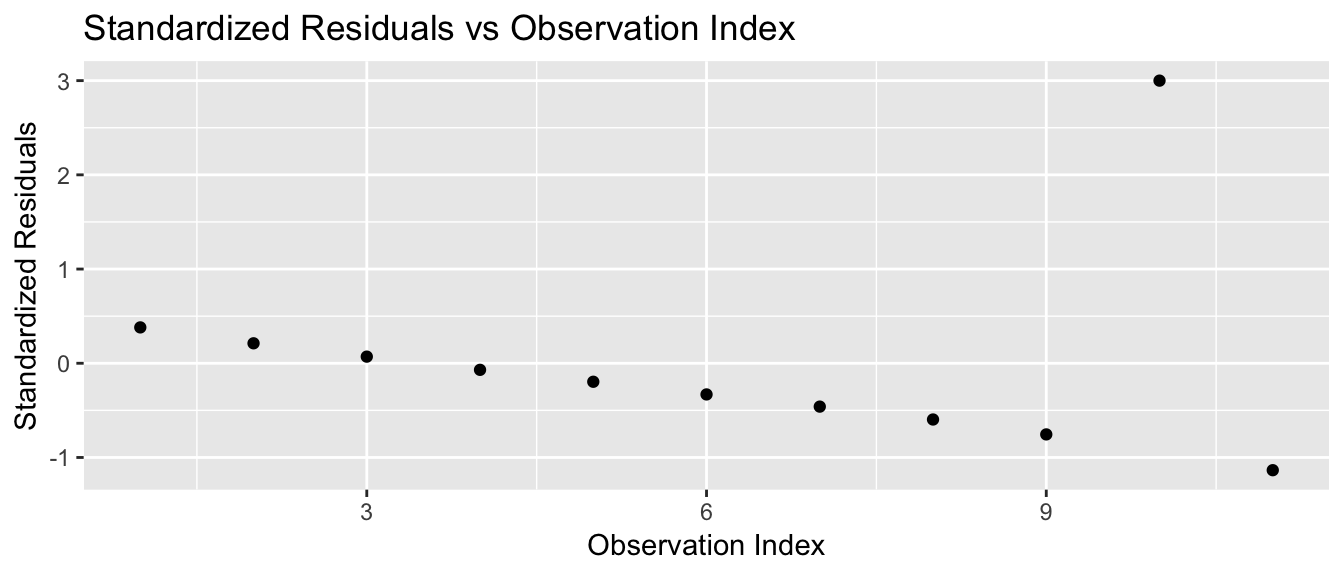
\includegraphics{Statistical_Methods_II_files/figure-latex/unnamed-chunk-98-1.pdf}

The red/blue lines going through the plot is a smoother of the
residuals. Ideally this should be a flat line and I should see no trend
in this plot. Clearly there is a quadratic trend as larger tortoises
have larger clutch sizes until some point where the extremely large
tortoises start laying fewer (perhaps the extremely large tortoises are
extremely old as well). To correct for this, we should fit a model that
is quadratic in \texttt{carapace\ length}. We will create a new
covariate, \texttt{carapace.2}, which is the square of the carapace
length and add it to the model.

In general I could write the quadratic model as
\[y_{i}=\beta_{0}+\beta_{1}x_{i}+\beta_{2}x_{i}^{2}+\epsilon_{i}\] and
note that my model is still a linear model with respect to covariates
\(\boldsymbol{x}\) and \(\boldsymbol{x}^{2}\) because I can still write
the model as \[\begin{aligned} \boldsymbol{y}    
  &=    \boldsymbol{X}\boldsymbol{\beta}+\boldsymbol{\epsilon} \\
    &=  \left[\begin{array}{ccc}
      1 & x_{1} & x_{1}^{2}\\
      1 & x_{2} & x_{2}^{2}\\
      1 & x_{3} & x_{3}^{2}\\
      \vdots & \vdots & \vdots\\
      1 & x_{n} & x_{n}^{2}
  \end{array}\right]\left[\begin{array}{c}
        \beta_{0}\\
        \beta_{1}\\
        \beta_{2}
\end{array}\right]
+
\left[\begin{array}{c}
\epsilon_{1}\\
\epsilon_{2}\\
\epsilon_{3}\\
\vdots\\
\epsilon_{n}
\end{array}\right]\end{aligned}\]

\begin{Shaded}
\begin{Highlighting}[]
\CommentTok{# add a new column that is carapace^2}
\NormalTok{Eggs2 <-}\StringTok{ }\NormalTok{Eggs %>%}\StringTok{ }\KeywordTok{mutate}\NormalTok{( }\DataTypeTok{carapace.2 =} \NormalTok{carapace^}\DecValTok{2} \NormalTok{)}
\NormalTok{model <-}\StringTok{ }\KeywordTok{lm}\NormalTok{( clutch.size ~}\StringTok{ }\NormalTok{carapace +}\StringTok{ }\NormalTok{carapace}\FloatTok{.2}\NormalTok{,    }\DataTypeTok{data=}\NormalTok{Eggs2 )}

\CommentTok{# make R do it inside the formula... convenient}
\NormalTok{model <-}\StringTok{ }\KeywordTok{lm}\NormalTok{( clutch.size ~}\StringTok{ }\NormalTok{carapace +}\StringTok{ }\KeywordTok{I}\NormalTok{(carapace^}\DecValTok{2}\NormalTok{), }\DataTypeTok{data=}\NormalTok{Eggs )}

\CommentTok{# Fit an arbitrary degree polynomial}
\NormalTok{model <-}\StringTok{ }\KeywordTok{lm}\NormalTok{( clutch.size ~}\StringTok{ }\KeywordTok{poly}\NormalTok{(carapace, }\DecValTok{2}\NormalTok{),        }\DataTypeTok{data=}\NormalTok{Eggs )}

\CommentTok{# If you use poly() in the formula, you must use 'data=' here, }
\CommentTok{# otherwise you can skip it and R will do the right thing.}
\KeywordTok{autoplot}\NormalTok{(model, }\DataTypeTok{which=}\DecValTok{1}\NormalTok{, }\DataTypeTok{data=}\NormalTok{Eggs)  }
\end{Highlighting}
\end{Shaded}

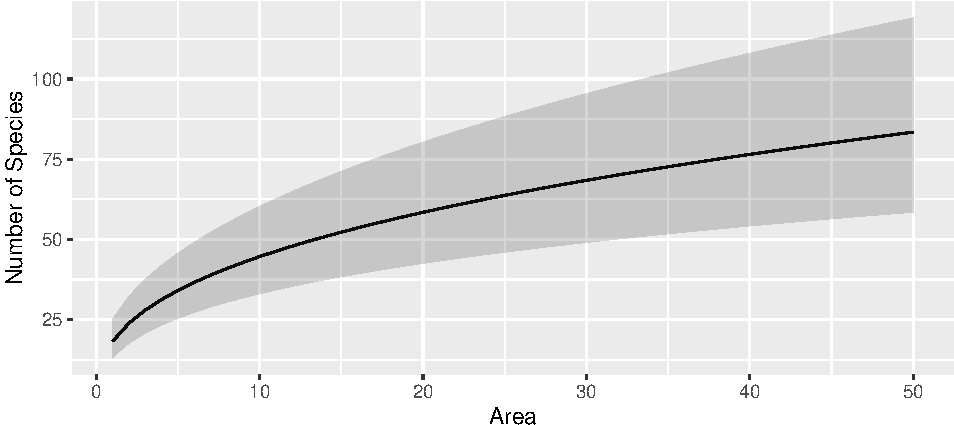
\includegraphics{Statistical_Methods_II_files/figure-latex/unnamed-chunk-99-1.pdf}

Now our residual plot versus fitted values does not show any trend,
suggesting that the quadratic model is fitting the data well. Graphing
the original data along with the predicted values confirms this.

\begin{Shaded}
\begin{Highlighting}[]
\CommentTok{# add the fitted and CI lwr/upr columns to my dataset }
\NormalTok{Eggs <-}\StringTok{ }\NormalTok{Eggs %>%}\StringTok{ }\KeywordTok{cbind}\NormalTok{( }\KeywordTok{predict}\NormalTok{(model, }\DataTypeTok{interval=}\StringTok{'confidence'}\NormalTok{) )}

\KeywordTok{ggplot}\NormalTok{(Eggs, }\KeywordTok{aes}\NormalTok{(}\DataTypeTok{x=}\NormalTok{carapace)) +}
\StringTok{  }\KeywordTok{geom_ribbon}\NormalTok{( }\KeywordTok{aes}\NormalTok{(}\DataTypeTok{ymin=}\NormalTok{lwr, }\DataTypeTok{ymax=}\NormalTok{upr), }\DataTypeTok{fill=}\StringTok{'red'}\NormalTok{, }\DataTypeTok{alpha=}\NormalTok{.}\DecValTok{3}\NormalTok{) +}
\StringTok{  }\KeywordTok{geom_line}\NormalTok{(}\KeywordTok{aes}\NormalTok{(}\DataTypeTok{y=}\NormalTok{fit), }\DataTypeTok{color=}\StringTok{'red'}\NormalTok{) +}
\StringTok{  }\KeywordTok{geom_point}\NormalTok{(}\KeywordTok{aes}\NormalTok{(}\DataTypeTok{y=}\NormalTok{clutch.size)) }
\end{Highlighting}
\end{Shaded}

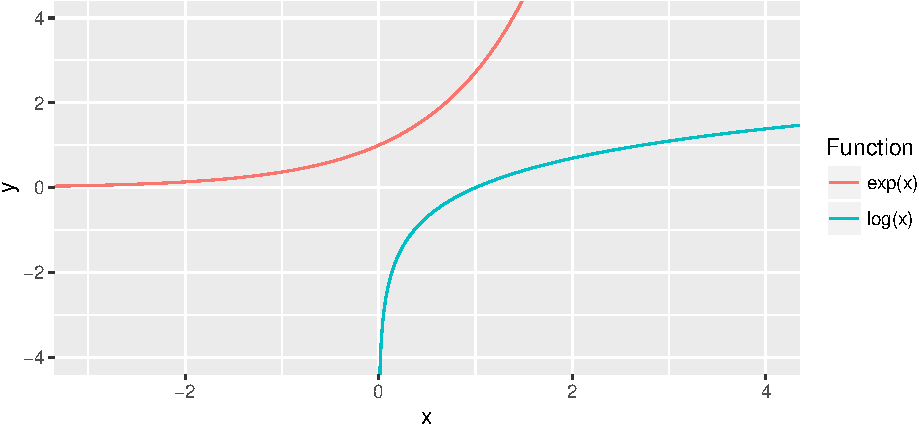
\includegraphics{Statistical_Methods_II_files/figure-latex/unnamed-chunk-100-1.pdf}

\paragraph{Heteroskedasticity}\label{heteroskedasticity}

The plot of residuals versus fitted values can detect heteroskedasticity
(non-constant variance) in the error terms.

To illustrate this, we turn to another dataset in the Faraway book. The
dataset airquality uses data taken from an environmental study that
measured four variables, ozone, solar radiation, temperature and
windspeed for 153 consecutive days in New York. The goal is to predict
the level of ozone using the weather variables.

We first graph all pairs of variables in the dataset.

\begin{Shaded}
\begin{Highlighting}[]
\KeywordTok{data}\NormalTok{(airquality)}
\KeywordTok{pairs}\NormalTok{(~}\StringTok{ }\NormalTok{Ozone +}\StringTok{ }\NormalTok{Solar.R +}\StringTok{ }\NormalTok{Wind +}\StringTok{ }\NormalTok{Temp, }\DataTypeTok{data=}\NormalTok{airquality)}
\end{Highlighting}
\end{Shaded}

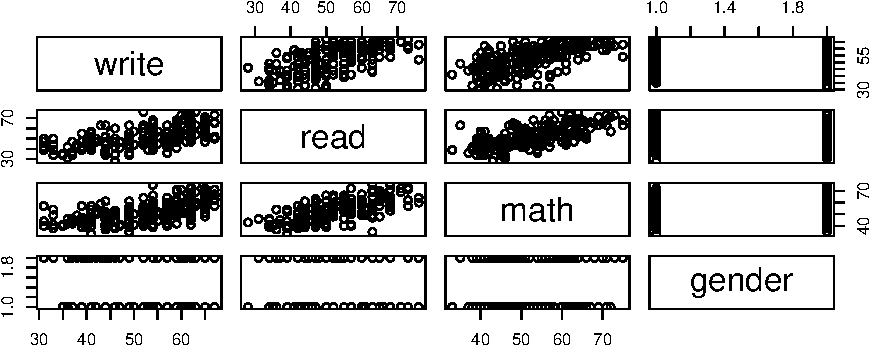
\includegraphics{Statistical_Methods_II_files/figure-latex/unnamed-chunk-101-1.pdf}

and notice that ozone levels are positively correlated with solar
radiation and temperature, and negatively correlated with wind speed. A
linear relationship with wind might be suspect as is the increasing
variability in the response to high temperature. However, we don't know
if those trends will remain after fitting the model, because there is
some covariance amongst the predictors.

\begin{Shaded}
\begin{Highlighting}[]
\NormalTok{model <-}\StringTok{ }\KeywordTok{lm}\NormalTok{(Ozone ~}\StringTok{ }\NormalTok{Solar.R +}\StringTok{ }\NormalTok{Wind +}\StringTok{ }\NormalTok{Temp, }\DataTypeTok{data=}\NormalTok{airquality)}
\KeywordTok{autoplot}\NormalTok{(model, }\DataTypeTok{which=}\DecValTok{1}\NormalTok{) }
\end{Highlighting}
\end{Shaded}

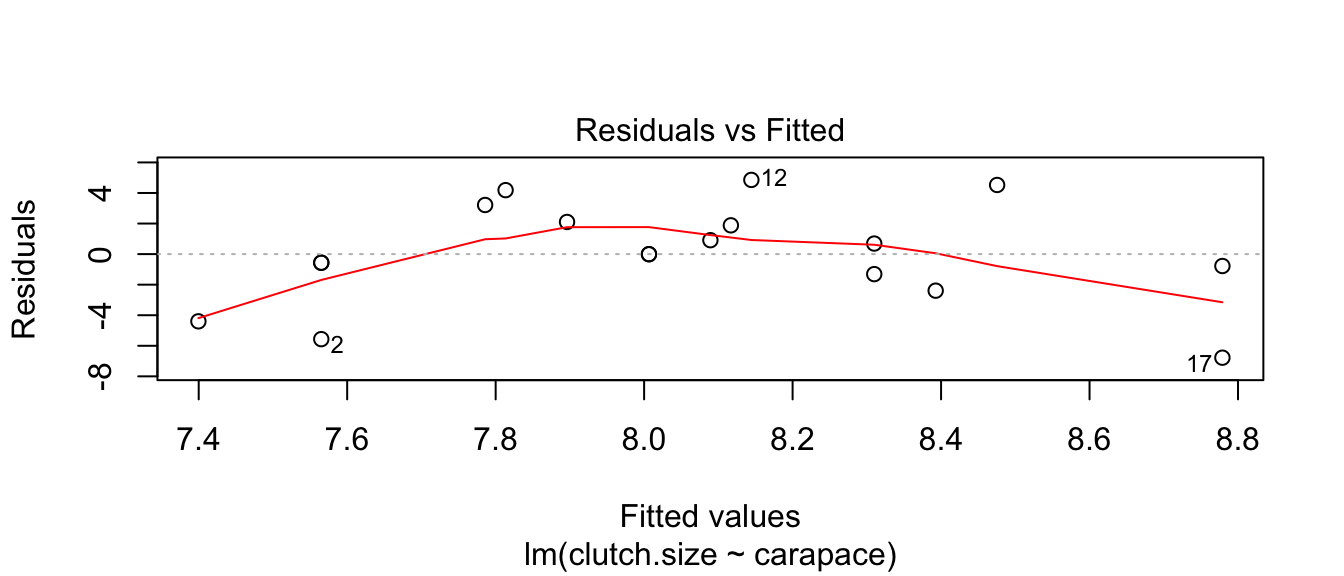
\includegraphics{Statistical_Methods_II_files/figure-latex/unnamed-chunk-102-1.pdf}

As we feared, we have both a non-constant variance and a non-linear
relationship. A transformation of the \(y\) variable might be able to
fix our problem.

\subsubsection{QQplots}\label{qqplots}

If we are taking a sample of size \(n=10\) from a standard normal
distribution, then I should expect that the smallest observation will be
negative. Intuitively, you would expect the smallest observation to be
near the \(10\)th percentile of the standard normal, and likewise the
second smallest should be near the \(20\)th percentile.

This idea needs a little modification because the largest observation
cannot be near the \(100\)th percentile (because that is \(\infty\)). So
we'll adjust the estimates to still be spaced at \((1/n)\) quantile
increments, but starting at the \(0.5/n\) quantile instead of the
\(1/n\) quantile. So the smallest observation should be near the
\(0.05\) quantile, the second smallest should be near the \(0.15\)
quantile, and the largest observation should be near the \(0.95\)
quantile. I will refer to these as the \emph{theoretical quantiles}.

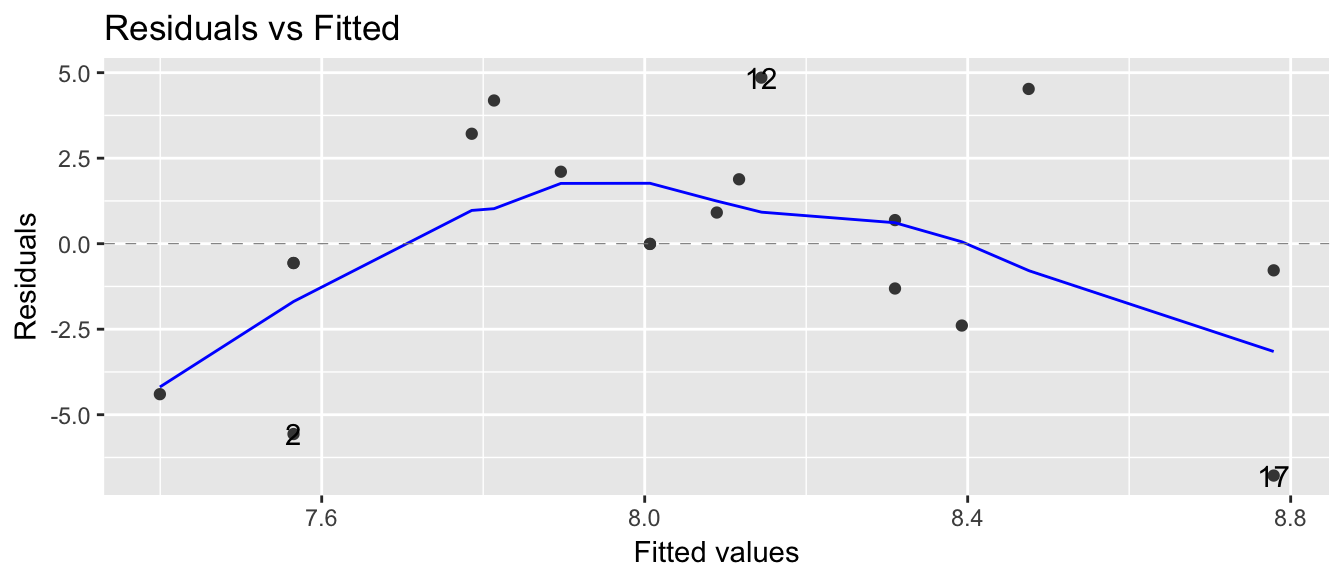
\includegraphics{Statistical_Methods_II_files/figure-latex/unnamed-chunk-103-1.pdf}

I can then graph the theoretical quantiles vs my observed values and if
they lie on the 1-to-1 line, then my data comes from a standard normal
distribution.

\begin{Shaded}
\begin{Highlighting}[]
\KeywordTok{set.seed}\NormalTok{(}\DecValTok{93516}\NormalTok{)  }\CommentTok{# make random sample in the next code chunk consistant run-to-run}

\NormalTok{n <-}\StringTok{ }\DecValTok{10}
\NormalTok{data <-}\StringTok{ }\KeywordTok{data.frame}\NormalTok{( }\DataTypeTok{observed =} \KeywordTok{rnorm}\NormalTok{(n, }\DataTypeTok{mean=}\DecValTok{0}\NormalTok{, }\DataTypeTok{sd=}\DecValTok{1}\NormalTok{) ) %>%}
\StringTok{  }\KeywordTok{arrange}\NormalTok{(observed) %>%}
\StringTok{  }\KeywordTok{mutate}\NormalTok{( }\DataTypeTok{theoretical =} \KeywordTok{qnorm}\NormalTok{( (}\DecValTok{1}\NormalTok{:n -.}\DecValTok{5}\NormalTok{)/n ) )}

\KeywordTok{ggplot}\NormalTok{(data, }\KeywordTok{aes}\NormalTok{(}\DataTypeTok{x=}\NormalTok{theoretical, }\DataTypeTok{y=}\NormalTok{observed) ) +}\StringTok{ }
\StringTok{  }\KeywordTok{geom_point}\NormalTok{() +}
\StringTok{  }\KeywordTok{geom_abline}\NormalTok{( }\DataTypeTok{intercept=}\DecValTok{0}\NormalTok{, }\DataTypeTok{slope=}\DecValTok{1}\NormalTok{,  }\DataTypeTok{linetype=}\DecValTok{2}\NormalTok{, }\DataTypeTok{alpha=}\NormalTok{.}\DecValTok{7}\NormalTok{) +}\StringTok{ }
\StringTok{  }\KeywordTok{labs}\NormalTok{(}\DataTypeTok{main=}\StringTok{'Q-Q Plot: Observed vs Normal Distribution'}\NormalTok{)}
\end{Highlighting}
\end{Shaded}

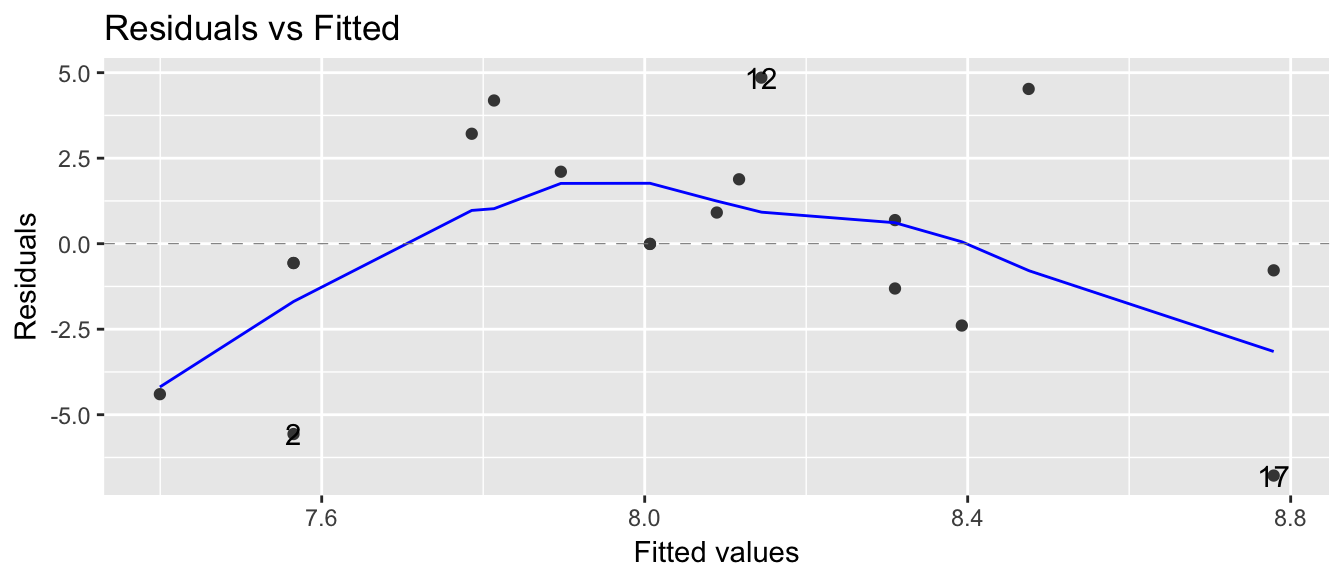
\includegraphics{Statistical_Methods_II_files/figure-latex/unnamed-chunk-104-1.pdf}

In the context of a regression model, we wish to look at the residuals
and see if there are obvious departures from normality. Returning to the
airquality example, R will calculate the qqplot for us.

\begin{Shaded}
\begin{Highlighting}[]
\NormalTok{model <-}\StringTok{ }\KeywordTok{lm}\NormalTok{(Ozone ~}\StringTok{ }\NormalTok{Solar.R +}\StringTok{ }\NormalTok{Wind +}\StringTok{ }\NormalTok{Temp, }\DataTypeTok{data=}\NormalTok{airquality)}
\KeywordTok{autoplot}\NormalTok{(model, }\DataTypeTok{which=}\DecValTok{2}\NormalTok{) }
\end{Highlighting}
\end{Shaded}

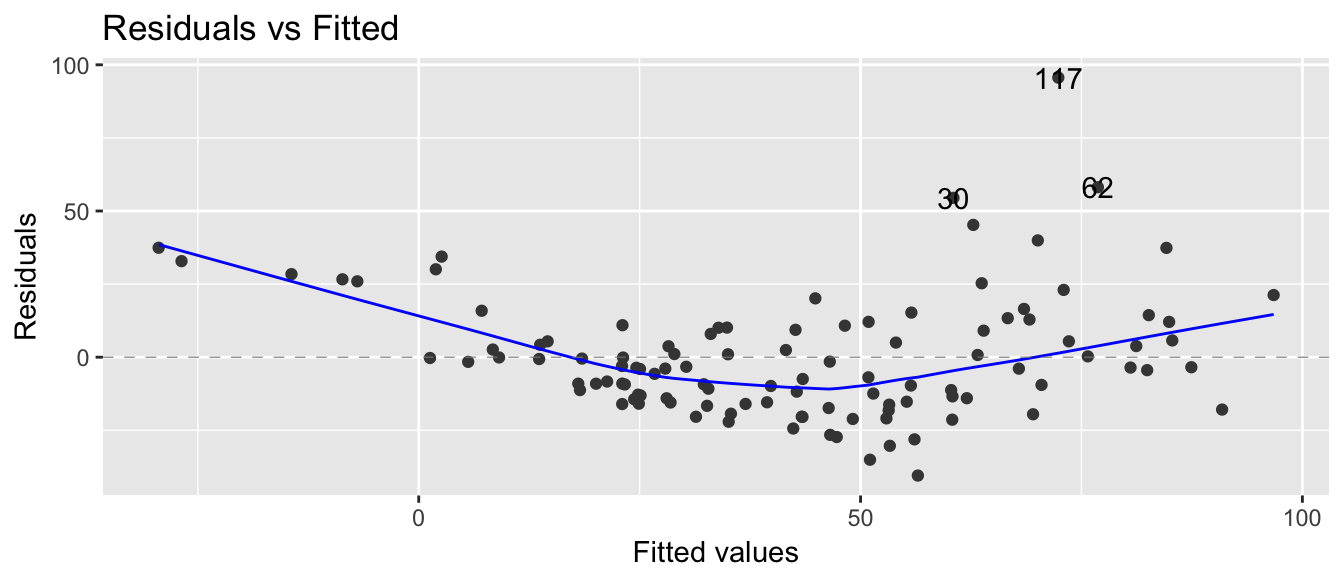
\includegraphics{Statistical_Methods_II_files/figure-latex/unnamed-chunk-105-1.pdf}

In this case, we have a large number of residuals that are bigger than I
would expect them to be based on them being from a normal distribution.
We could further test this using the Shapiro-Wilks test and compare the
standardized residuals against a \(N\left(0,1\right)\) distribution.

\begin{Shaded}
\begin{Highlighting}[]
\KeywordTok{shapiro.test}\NormalTok{( }\KeywordTok{rstandard}\NormalTok{(model) )}
\end{Highlighting}
\end{Shaded}

\begin{verbatim}
## 
##  Shapiro-Wilk normality test
## 
## data:  rstandard(model)
## W = 0.9151, p-value = 2.819e-06
\end{verbatim}

The tail of the distribution of observed residuals is \emph{far} from
what we expect to see.

\subsubsection{Scale-Location Plot}\label{scale-location-plot}

This plot is a variation on the fitted vs residuals plot, but the y-axis
uses the square root of the absolute value of the standardized
residuals. Supposedly this makes detecting increasing variance easier to
detect, but I'm not convinced.

\subsubsection{Residuals vs Leverage (plus Cook's
Distance)}\label{residuals-vs-leverage-plus-cooks-distance}

This plot lets the user examine the which observations have a high
potential for being influential (i.e.~high leverage) versus how large
the residual is. Because Cook's distance is a function of those two
traits, we can also divide the graph up into regions by the value of
Cook's Distance.

Returning to Anscombe's third set of data, we see

\textless{}\textless{}\textgreater{}\textgreater{}=

\begin{Shaded}
\begin{Highlighting}[]
\NormalTok{model3 <-}\StringTok{ }\KeywordTok{lm}\NormalTok{(y ~}\StringTok{ }\NormalTok{x, }\DataTypeTok{data=}\NormalTok{Set3)}
\KeywordTok{autoplot}\NormalTok{(model3, }\DataTypeTok{which=}\DecValTok{5}\NormalTok{)}
\end{Highlighting}
\end{Shaded}

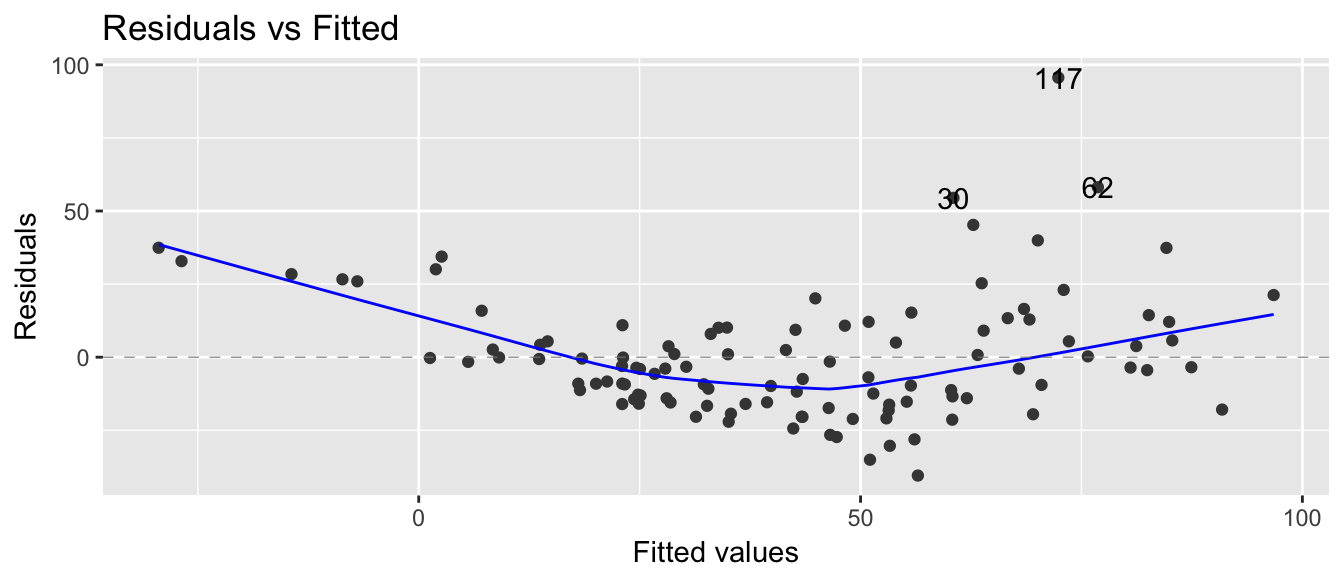
\includegraphics{Statistical_Methods_II_files/figure-latex/unnamed-chunk-107-1.pdf}

that one data point (observation 10) has an extremely large standardized
residual. This is one plot where I prefer what the base graphics in R
does compared to the ggfortify version. The base version of R adds some
contour lines that mark where the contours of where Cook's distance is
1/2 and 1.

\begin{Shaded}
\begin{Highlighting}[]
\KeywordTok{plot}\NormalTok{(model3, }\DataTypeTok{which=}\DecValTok{5}\NormalTok{)}
\end{Highlighting}
\end{Shaded}

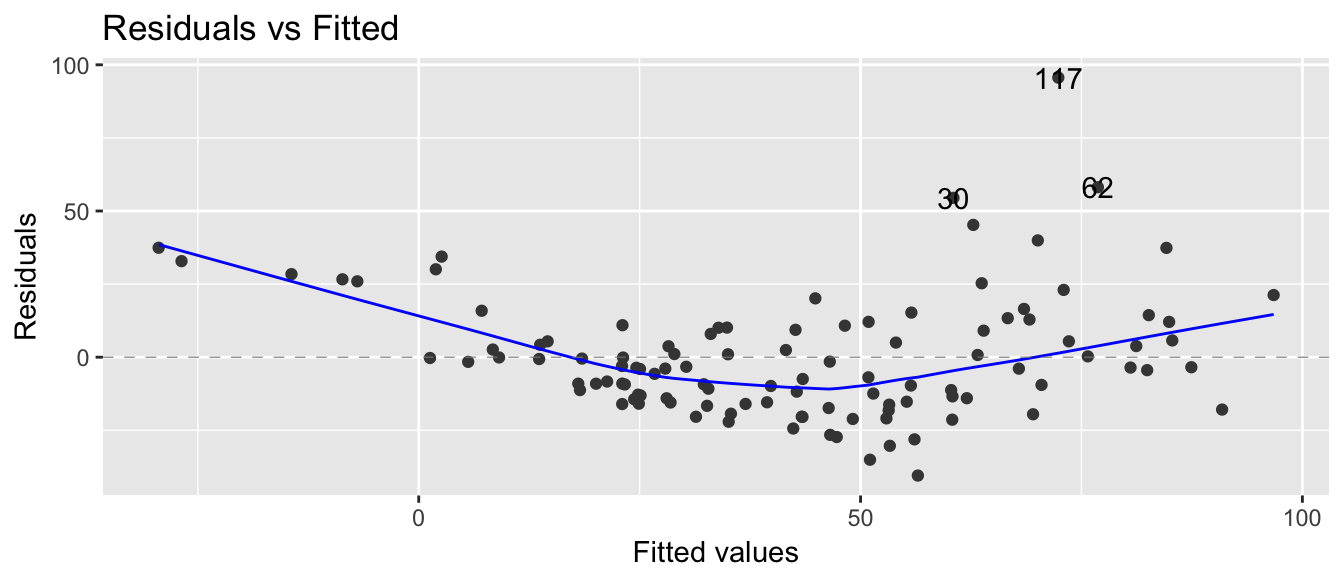
\includegraphics{Statistical_Methods_II_files/figure-latex/unnamed-chunk-108-1.pdf}

\section{Transformations}\label{transformations}

Transformations of the response variable and/or the predictor variables
can drastically improve the model fit and can correct violations of the
model assumptions. We might also create new predictor variables that are
functions of existing variables. These include quadratic and higher
order polynomial terms and interaction terms.

Often we are presented with data and we would like to fit a linear model
to the data. Unfortunately the data might not satisfy all of the
assumptions of a linear model. For the simple linear model
\[y=\beta_{0}+\beta_{1}x+\epsilon\] where
\(\epsilon\sim N\left(0,\sigma^{2}\right)\), the necessary assumptions
are:

\begin{enumerate}
\def\labelenumi{\arabic{enumi}.}
\tightlist
\item
  Independent errors
\item
  Errors have constant variance, no matter what the x-value (or
  equivalently the fitted value)
\item
  Errors are normally distributed
\item
  The model contains all the appropriate covariates and no more.
\end{enumerate}

In general, a transformation of the response variable can be used to
address the 2nd and 3rd assumptions, and adding new covariates to the
model will be how to address deficiencies of assumption 4.

\subsection{Transforming the Response}\label{transforming-the-response}

When the normality or constant variance assumption is violated,
sometimes it is possible to transform the response to satisfy the
assumption. Often times count data is analyzed as \texttt{log(count)}
and weights are analyzed after taking a square root or cube root
transform. Statistics involving income or other monetary values are
usually analyzed on the log scale so as to reduce the leverage of high
income observations.

While we may want to transform the response in order to satisfy the
statistical assumptions, it is often necessary to back-transform to the
original scale. For example if we fit a linear model for income (\(y\))
based on the amount of schooling the individual has received (\(x\))
\[\log y=\beta_{0}+\beta_{1}x+\epsilon\] then we might want to give a
prediction interval for an \(x_{0}\) value. The predicted
\(log(income)\) value is
\[\log\left(\hat{y}_{0}\right)=\hat{\beta}_{0}+\hat{\beta}_{x}x_{0}\]
and we could calculate the appropriate predicted income as
\(\hat{y}_{0}=e^{log\left(\hat{y}_{0}\right)}\). Likewise if we had a
confidence interval or prediction interval for
\(\log\left(\hat{y}_{0}\right)\) of the form \(\left(l,u\right)\) then
the appropriate interval for \(\hat{y}_{0}\) is
\(\left(e^{l},e^{u}\right)\). Notice that while \(\left(l,u\right)\)
might be symmetric about \(\log\left(\hat{y}_{0}\right)\), the
back-transformed interval is not symmetric about \(\hat{y}_{0}\).

Unfortunately the interpretation of the regression coefficients
\(\hat{\beta}_{0}\) and \(\hat{\beta}_{1}\) on the untransformed scale
becomes more complicated. This is a very serious difficulty and might
sway a researcher from transforming their data.

\subsubsection{Box-Cox Family of
Transformations}\label{box-cox-family-of-transformations}

The Box-Cox method is a popular way of determining what transformation
to make. It is intended for responses that are strictly positive
(because \(\log0=-\infty\) and the square root of a number gives complex
numbers, which we don't know how to address in regression). The
transformation is defined as \[g\left(y\right)=\begin{cases}
\frac{y^{\lambda}-1}{\lambda} & \lambda\ne0\\
\log y & \lambda=0
\end{cases}\] This transformation is a smooth family of transformations
because \[\lim_{\lambda\to0}\frac{y^{\lambda}-1}{\lambda}=\log y\] In
the case that \(\lambda\ne 0\), then a researcher will usually use the
simpler transformation \(y^{\lambda}\) because the subtraction and
division does not change anything in a non-linear fashion. Thus for
purposes of addressing the assumption violations, all we care about is
the \(y^{\lambda}\) and prefer the simpler (i.e.~more interpretable)
transformation.

Finding the best transformation can be done by adding the \(\lambda\)
parameter to the model and finding the value that maximizes the
log-likelihood function. Fortunately, we don't have to do this by hand,
as the function \texttt{boxcox()} in the \texttt{MASS} library will do
all the heavy calculation for us.

\begin{Shaded}
\begin{Highlighting}[]
\KeywordTok{library}\NormalTok{(faraway)}
\KeywordTok{library}\NormalTok{(MASS)}
\KeywordTok{data}\NormalTok{(gala)}
\NormalTok{g <-}\StringTok{ }\KeywordTok{lm}\NormalTok{(Species ~}\StringTok{ }\NormalTok{Area +}\StringTok{ }\NormalTok{Elevation +}\StringTok{ }\NormalTok{Nearest +}\StringTok{ }\NormalTok{Scruz +}\StringTok{ }\NormalTok{Adjacent, }\DataTypeTok{data=}\NormalTok{gala)}
\KeywordTok{boxcox}\NormalTok{(g)}
\end{Highlighting}
\end{Shaded}

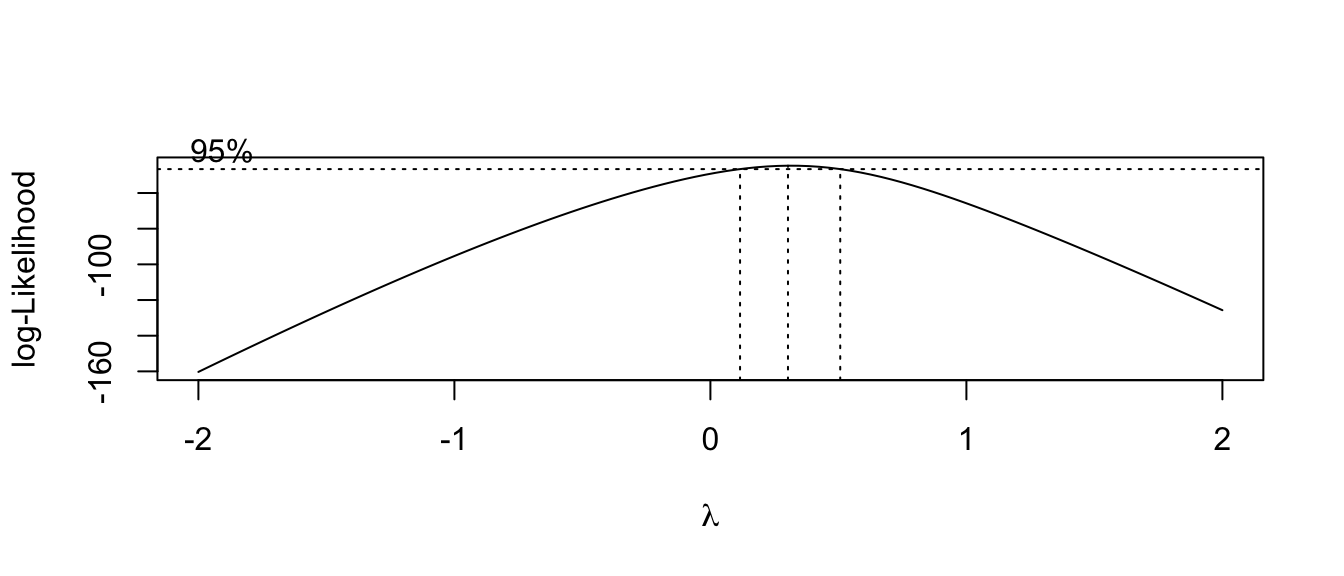
\includegraphics{Statistical_Methods_II_files/figure-latex/unnamed-chunk-109-1.pdf}

The optimal transformation for these data would be
\(y^{1/4}=\sqrt[4]{y}\) but that is an extremely uncommon
transformation. Instead we should pick the nearest ``standard''
transformation which would suggest that we should use either the
\(\log y\) or \(\sqrt{y}\) transformation.

Thoughts on the Box-Cox transformation:

\begin{enumerate}
\def\labelenumi{\arabic{enumi}.}
\tightlist
\item
  In general, I prefer to using a larger-than-optimal model when picking
  a transformation and then go about the model building process. After a
  suitable model has been chosen, I'll double check the my
  transformation was appropriate given the model that I ended up with.
\item
  Outliers can have a profound effect on this method. If the ``optimal''
  transformation is extreme (\(\lambda=5\) or something silly) then you
  might have to remove the outliers and refit the transformation.
\item
  If the range of the response \(y\) is small, then the method is not as
  sensitive.
\item
  These are not the only possible transformations. For example, for
  binary data, the \texttt{logit} and \texttt{probit} transformations
  are common.
\end{enumerate}

\subsection{Transforming the
predictors}\label{transforming-the-predictors}

\subsubsection{Polynomials of a
predictor}\label{polynomials-of-a-predictor}

Perhaps the most common transformation to make is to make a quadratic
function in \(x\). Often the relationship between \(x\) and \(y\)
follows a curve and we want to fit a quadratic model
\[\hat{y}=\hat{\beta}_{0}+\hat{\beta}_{1}x+\hat{\beta}_{2}x^{2}\] and we
should note that this is still a linear model because \(\hat{y}\) is a
linear function of \(x\) and \(x^{2}\). As we have already seen, it is
easy to fit the model. Adding the column of \(x^{2}\) values to the
design matrix does the trick.

The difficult part comes in the interpretation of the parameter values.
No longer is \(\hat{\beta}_{1}\) the increase in \(y\) for every one
unit increase in \(x\). Instead the three parameters in my model
interact in a complicated fashion. For example, the peak of the parabola
is at \(-\hat{\beta}_{1}/2\hat{\beta}_{2}\) and whether the parabola is
cup shaped vs dome shaped and its steepness is controlled by
\(\hat{\beta}_{2}\). Because my geometric understanding of degree \(q\)
polynomials relies on have all factors of degree \(q\) or lower,
whenever I include a covariate raised to a power, I should include all
the lower powers as well.

\subsubsection{Log and Square Root of a
predictor}\label{log-and-square-root-of-a-predictor}

Often the effect of a covariate is not linearly related to response, but
rather some function of the covariate. For example the area of a circle
is not linearly related to its radius, but it is linearly related to the
radius squared. \[Area=\pi r^{2}\] Similar situations might arise in
biological settings, such as the volume of conducting tissue being
related to the square of the diameter. Or perhaps an animals metabolic
requirements are related to some power of body length. In sociology, it
is often seen that the utility of, say, \$1000 drops off in a
logarithmic fashion according to the person's income. To a graduate
student, \$1K is a big deal, but to a corporate CEO, \$1K is just
another weekend at the track. Making a log transformation on any
monetary covariate, might account for the non-linear nature of
``utility''.

Picking a good transformation for a covariate is quite difficult, but
most fields of study have spent plenty of time thinking about these
issues. When in doubt, look at scatter plots of the covariate vs the
response and ask what transformation would make the data fall onto a
line?

\subsubsection{Examples of transformation of
predictors}\label{examples-of-transformation-of-predictors}

To illustrate how to add a transformation of a predictor to a linear
model in R, we will consider the Galapagos data in \texttt{faraway}.

\begin{Shaded}
\begin{Highlighting}[]
\KeywordTok{library}\NormalTok{(faraway)}
\KeywordTok{data}\NormalTok{(gala)}
\CommentTok{# look at all the scatterplots}
\KeywordTok{pairs}\NormalTok{(}\KeywordTok{log}\NormalTok{(Species) ~}\StringTok{ }\NormalTok{Area +}\StringTok{ }\NormalTok{Elevation +}\StringTok{ }\NormalTok{Nearest +}\StringTok{ }\NormalTok{Scruz +}\StringTok{ }\NormalTok{Adjacent, }\DataTypeTok{data=}\NormalTok{gala)}
\end{Highlighting}
\end{Shaded}

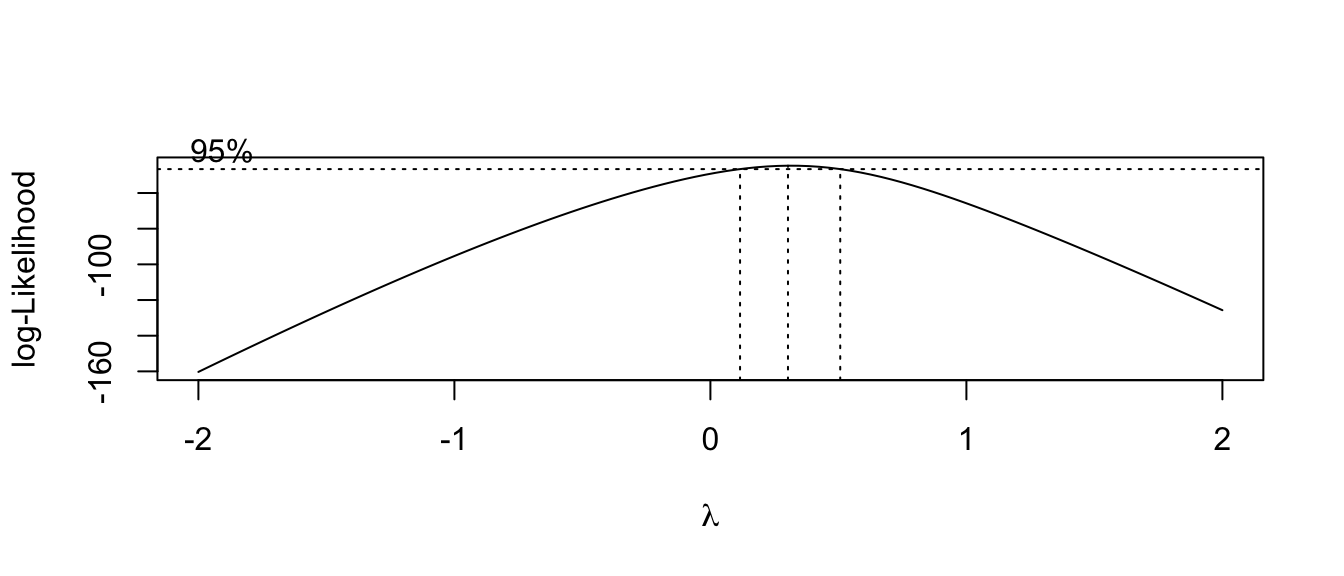
\includegraphics{Statistical_Methods_II_files/figure-latex/unnamed-chunk-110-1.pdf}

Looking at these graphs, I think I should transform \texttt{elevation},
\texttt{Adjacent}, and \texttt{Area} and perhaps a log transformation is
a good idea.

\begin{Shaded}
\begin{Highlighting}[]
\KeywordTok{pairs}\NormalTok{( }\KeywordTok{log}\NormalTok{(Species) ~}\StringTok{ }\KeywordTok{log}\NormalTok{(Elevation) +}\StringTok{ }\KeywordTok{log}\NormalTok{(Area) +}\StringTok{ }
\StringTok{                       }\NormalTok{Nearest +}\StringTok{ }\NormalTok{Scruz +}\StringTok{ }\KeywordTok{log}\NormalTok{(Adjacent), }\DataTypeTok{data=}\NormalTok{gala)}
\end{Highlighting}
\end{Shaded}

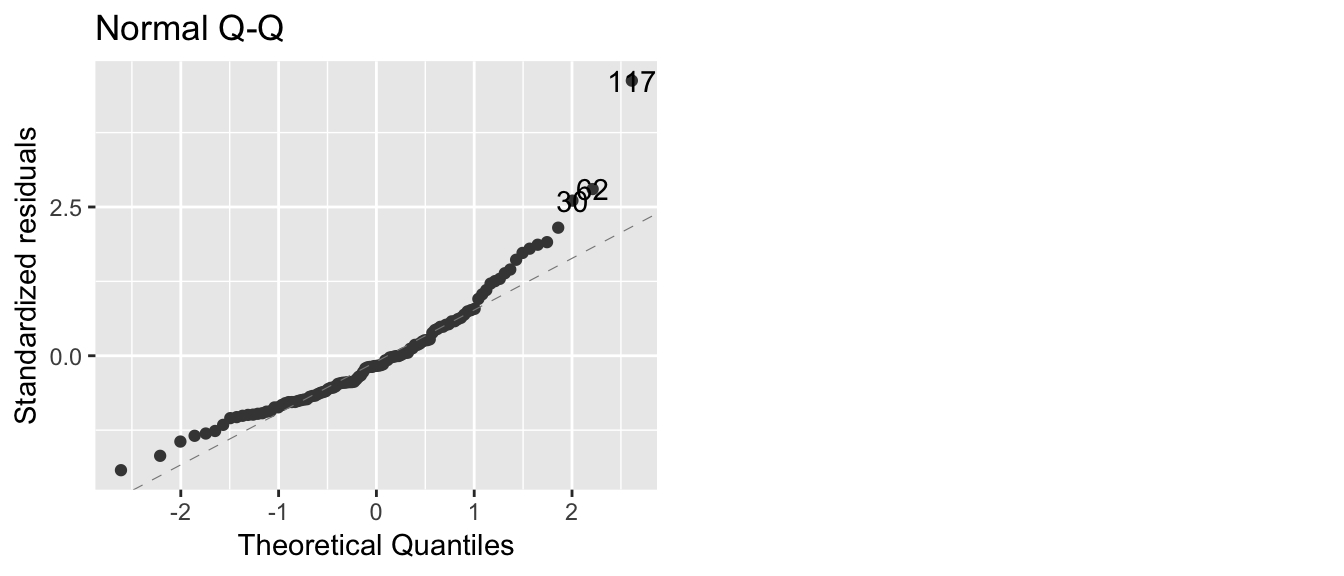
\includegraphics{Statistical_Methods_II_files/figure-latex/unnamed-chunk-111-1.pdf}

Looking at these graphs, it is clear that \texttt{log(Elevation)} and
\texttt{log(Area)} are highly correlated and we should probably have one
or the other, but not both in the model.

\begin{Shaded}
\begin{Highlighting}[]
\NormalTok{m.c <-}\StringTok{ }\KeywordTok{lm}\NormalTok{(}\KeywordTok{log}\NormalTok{(Species) ~}\StringTok{  }\KeywordTok{log}\NormalTok{(Area) +}\StringTok{ }\NormalTok{Nearest +}\StringTok{ }\NormalTok{Scruz +}\StringTok{ }\KeywordTok{log}\NormalTok{(Adjacent), }\DataTypeTok{data=}\NormalTok{gala)}
\KeywordTok{summary}\NormalTok{(m.c)$coefficients %>%}\StringTok{ }\KeywordTok{round}\NormalTok{(}\DataTypeTok{digits=}\DecValTok{3}\NormalTok{) }\CommentTok{# more readable...}
\end{Highlighting}
\end{Shaded}

\begin{verbatim}
##               Estimate Std. Error t value Pr(>|t|)
## (Intercept)      3.122      0.208  14.979    0.000
## log(Area)        0.398      0.044   9.027    0.000
## Nearest          0.000      0.013  -0.022    0.983
## Scruz           -0.003      0.003  -1.238    0.227
## log(Adjacent)   -0.021      0.045  -0.468    0.644
\end{verbatim}

We will remove all the parameters that appear to be superfluous, and
perorm an F-test to confirm that the simple model is sufficient.

\begin{Shaded}
\begin{Highlighting}[]
\NormalTok{m.s <-}\StringTok{ }\KeywordTok{lm}\NormalTok{(}\KeywordTok{log}\NormalTok{(Species) ~}\StringTok{ }\KeywordTok{log}\NormalTok{(Area), }\DataTypeTok{data=}\NormalTok{gala)}
\KeywordTok{anova}\NormalTok{(m.s, m.c)}
\end{Highlighting}
\end{Shaded}

\begin{verbatim}
## Analysis of Variance Table
## 
## Model 1: log(Species) ~ log(Area)
## Model 2: log(Species) ~ log(Area) + Nearest + Scruz + log(Adjacent)
##   Res.Df    RSS Df Sum of Sq      F Pr(>F)
## 1     28 17.218                           
## 2     25 15.501  3    1.7176 0.9234 0.4439
\end{verbatim}

Next we will look at the coefficients.

\begin{Shaded}
\begin{Highlighting}[]
\KeywordTok{summary}\NormalTok{(m.s)}
\end{Highlighting}
\end{Shaded}

\begin{verbatim}
## 
## Call:
## lm(formula = log(Species) ~ log(Area), data = gala)
## 
## Residuals:
##     Min      1Q  Median      3Q     Max 
## -1.5442 -0.4001  0.0941  0.5449  1.3752 
## 
## Coefficients:
##             Estimate Std. Error t value Pr(>|t|)    
## (Intercept)   2.9037     0.1571  18.484  < 2e-16 ***
## log(Area)     0.3886     0.0416   9.342 4.23e-10 ***
## ---
## Signif. codes:  0 '***' 0.001 '**' 0.01 '*' 0.05 '.' 0.1 ' ' 1
## 
## Residual standard error: 0.7842 on 28 degrees of freedom
## Multiple R-squared:  0.7571, Adjusted R-squared:  0.7484 
## F-statistic: 87.27 on 1 and 28 DF,  p-value: 4.23e-10
\end{verbatim}

The slope coefficient (0.3886) is the increase in log(Species) for every
1 unit increase in log(Area). Unfortunately that is not particularly
convenient to interpretation and we will address this in the next
section of this chapter.

Finally, we might be interested in creating a confidence interval for
the expected number of tortoise species for an island with
\texttt{Area=50}.

\begin{Shaded}
\begin{Highlighting}[]
\NormalTok{x0 <-}\StringTok{ }\KeywordTok{data.frame}\NormalTok{(}\DataTypeTok{Area=}\DecValTok{50}\NormalTok{)}
\NormalTok{log.Species.CI <-}\StringTok{ }\KeywordTok{predict}\NormalTok{(m.s, }\DataTypeTok{newdata=}\NormalTok{x0, }\DataTypeTok{interval=}\StringTok{'confidence'}\NormalTok{)}
\NormalTok{log.Species.CI       }\CommentTok{# Log(Species) scale}
\end{Highlighting}
\end{Shaded}

\begin{verbatim}
##        fit      lwr      upr
## 1 4.423903 4.068412 4.779394
\end{verbatim}

\begin{Shaded}
\begin{Highlighting}[]
\KeywordTok{exp}\NormalTok{(log.Species.CI)  }\CommentTok{# Species scale}
\end{Highlighting}
\end{Shaded}

\begin{verbatim}
##        fit      lwr      upr
## 1 83.42122 58.46403 119.0322
\end{verbatim}

Notice that on the species-scale, we see that the fitted value is not in
the center of the confidence interval.

To help us understand what the log transformations are doing, we can
produce a plot with the island Area on the x-axis and the expected
number of Species on the y-axis and hopefully that will help us
understand the relationship between the two.

\begin{Shaded}
\begin{Highlighting}[]
\KeywordTok{library}\NormalTok{(ggplot2)}
\NormalTok{pred.data <-}\StringTok{ }\KeywordTok{data.frame}\NormalTok{(}\DataTypeTok{Area=}\DecValTok{1}\NormalTok{:}\DecValTok{50}\NormalTok{)}
\NormalTok{pred.data <-}\StringTok{ }\NormalTok{pred.data %>%}\StringTok{ }\KeywordTok{cbind}\NormalTok{( }\KeywordTok{predict}\NormalTok{(m.s, }\DataTypeTok{newdata=}\NormalTok{pred.data, }\DataTypeTok{interval=}\StringTok{'conf'}\NormalTok{))}
\KeywordTok{ggplot}\NormalTok{(pred.data, }\KeywordTok{aes}\NormalTok{(}\DataTypeTok{x=}\NormalTok{Area)) +}
\StringTok{  }\KeywordTok{geom_line}\NormalTok{(}\KeywordTok{aes}\NormalTok{(}\DataTypeTok{y=}\KeywordTok{exp}\NormalTok{(fit))) +}
\StringTok{  }\KeywordTok{geom_ribbon}\NormalTok{(}\KeywordTok{aes}\NormalTok{(}\DataTypeTok{ymin=}\KeywordTok{exp}\NormalTok{(lwr), }\DataTypeTok{ymax=}\KeywordTok{exp}\NormalTok{(upr)), }\DataTypeTok{alpha=}\NormalTok{.}\DecValTok{2}\NormalTok{) +}
\StringTok{  }\KeywordTok{ylab}\NormalTok{(}\StringTok{'Number of Species'}\NormalTok{)}
\end{Highlighting}
\end{Shaded}

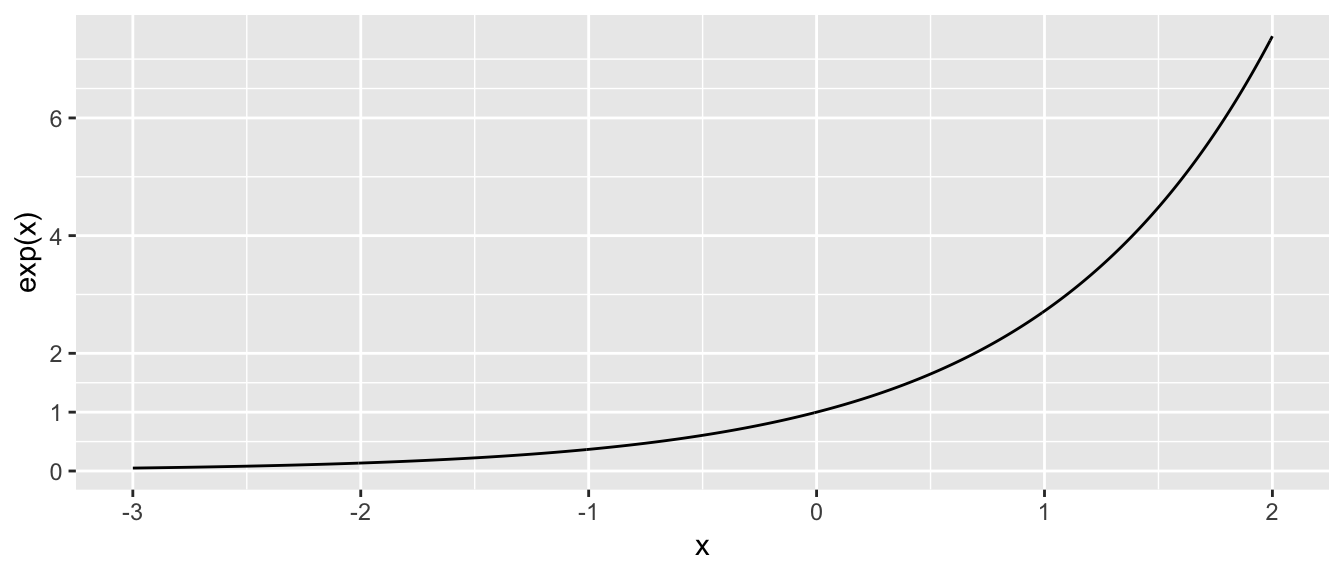
\includegraphics{Statistical_Methods_II_files/figure-latex/unnamed-chunk-116-1.pdf}

\subsection{Interpretation of log transformed
variables}\label{interpretation-of-log-transformed-variables}

One of the most difficult issues surrounding transformed variables is
that the interpretation is difficult. Here we look at the interpretation
of log transformed variables.

To begin with, we need to remind ourselves of what the functions
\(\log x\) and \(e^{x}\) look like.

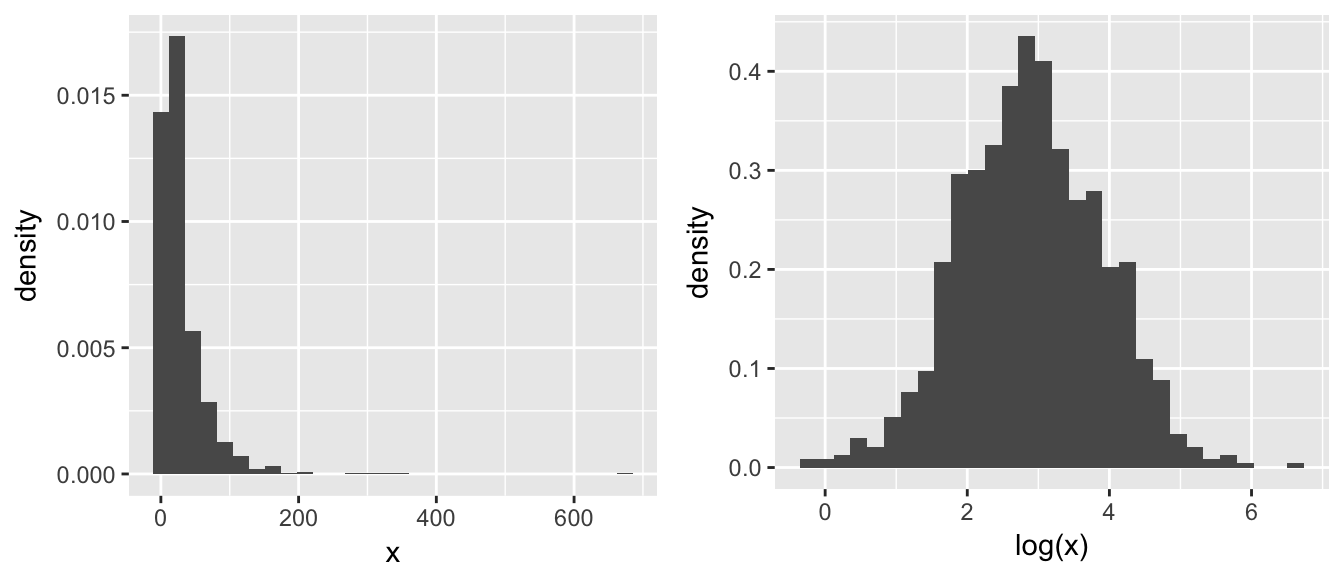
\includegraphics{Statistical_Methods_II_files/figure-latex/unnamed-chunk-117-1.pdf}

In particular we notice that \[e^{0}=1\] and \[\log\left(1\right)=0\]
and the functions \(e^{x}\) and \(\log x\) are inverse functions of each
other.

\[e^{\log x}=\log\left(e^{x}\right)=x\]

Also it is important to note that the \(\log\) function has some
interesting properties in that it makes operations ``1-operation
easier''. \[\begin{aligned} 
\log\left(a^{b}\right)        &=    b\log a  \\
\log\left(\frac{a}{b}\right)    &=  \log a-\log b \\
\log\left(ab\right)           &=    \log a+\log b
\end{aligned}\]

To investigate the effects of a log transformation, we'll examine a
dataset that predicts the writing scores of \(n=200\) students using the
gender, reading and math scores. This example was taken from the UCLA
Statistical Consulting Group.

\begin{Shaded}
\begin{Highlighting}[]
\NormalTok{scores <-}\StringTok{ }\KeywordTok{read.table}\NormalTok{(}
  \DataTypeTok{file=}\StringTok{'https://stats.idre.ucla.edu/wp-content/uploads/2016/02/lgtrans.csv'}\NormalTok{,}
  \DataTypeTok{header=}\OtherTok{TRUE}\NormalTok{, }\DataTypeTok{sep=}\StringTok{','}\NormalTok{)}
\NormalTok{scores <-}\StringTok{ }\NormalTok{scores %>%}\StringTok{ }\KeywordTok{mutate}\NormalTok{(}\DataTypeTok{gender =} \NormalTok{female)}
\KeywordTok{pairs}\NormalTok{(write~read+math+gender, }\DataTypeTok{data=}\NormalTok{scores)}
\end{Highlighting}
\end{Shaded}

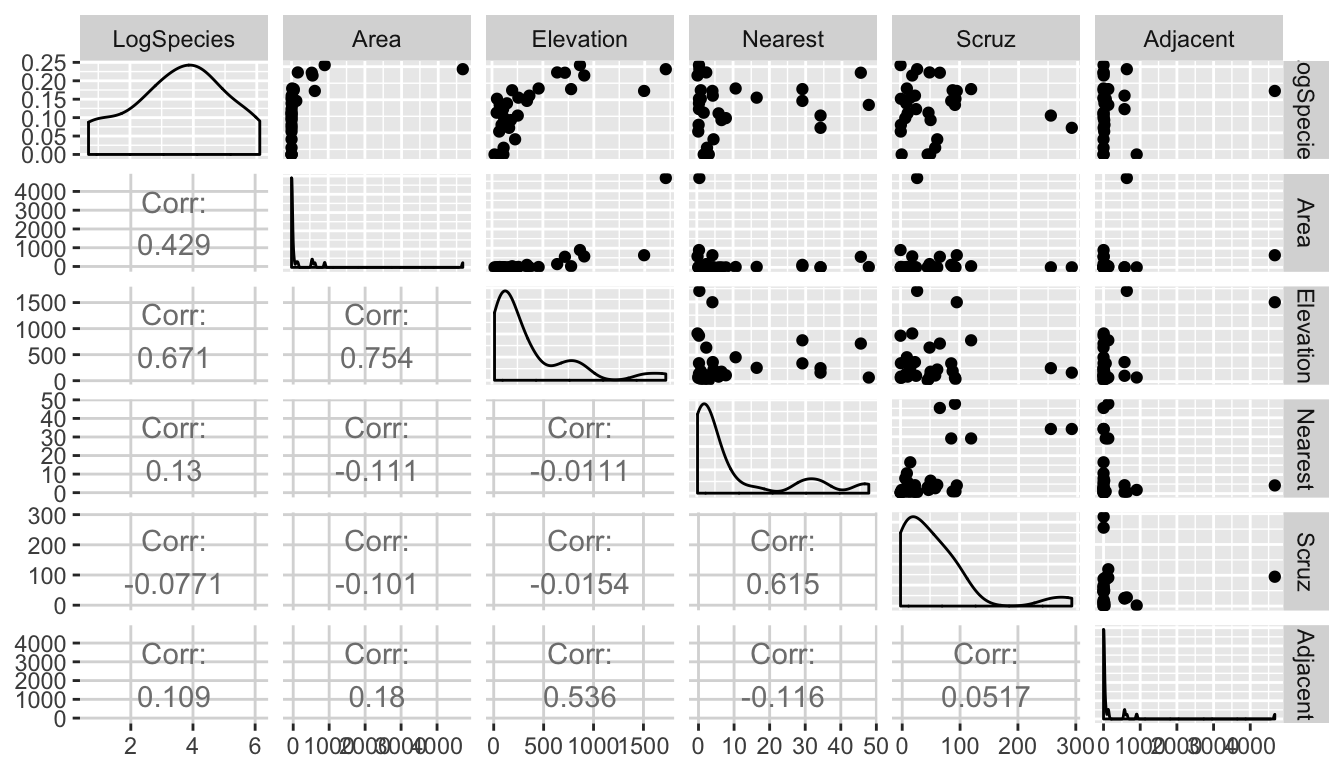
\includegraphics{Statistical_Methods_II_files/figure-latex/unnamed-chunk-118-1.pdf}

\subsubsection{Log-transformed response, untransformed
covariates}\label{log-transformed-response-untransformed-covariates}

We consider the model where we have transformed the response variable
and just an intercept term. \[\log y=\beta_{0}+\epsilon\]

\begin{Shaded}
\begin{Highlighting}[]
\NormalTok{m <-}\StringTok{ }\KeywordTok{lm}\NormalTok{(}\KeywordTok{log}\NormalTok{(write) ~}\StringTok{ }\DecValTok{1}\NormalTok{, }\DataTypeTok{data=}\NormalTok{scores)}
\KeywordTok{summary}\NormalTok{(m)$coef %>%}\StringTok{ }\KeywordTok{round}\NormalTok{(}\DataTypeTok{digits=}\DecValTok{3}\NormalTok{)}
\end{Highlighting}
\end{Shaded}

\begin{verbatim}
##             Estimate Std. Error t value Pr(>|t|)
## (Intercept)    3.948      0.014 288.402        0
\end{verbatim}

We interpret the intercept as the mean of the log-transformed response
values. We could back transform this to the original scale
\(\hat{y} = e^{\hat{\beta}_{0}} = e^{3.948} = 51.83\) as a typical value
of write. To distinguish this from the usually defined mean of the write
values, we will call this as the \emph{geometric mean}.

Next we examine how to interpret the model when a categorical variable
is added to the model. \[\log y=\begin{cases}
\beta_{0}+\epsilon & \;\;\textrm{if female}\\
\beta_{0}+\beta_{1}+\epsilon & \;\;\textrm{if male}
\end{cases}\]

\begin{Shaded}
\begin{Highlighting}[]
\NormalTok{m <-}\StringTok{ }\KeywordTok{lm}\NormalTok{(}\KeywordTok{log}\NormalTok{(write) ~}\StringTok{ }\NormalTok{gender, }\DataTypeTok{data=}\NormalTok{scores)}
\KeywordTok{summary}\NormalTok{(m)$coef %>%}\StringTok{ }\KeywordTok{round}\NormalTok{(}\DataTypeTok{digits=}\DecValTok{3}\NormalTok{)}
\end{Highlighting}
\end{Shaded}

\begin{verbatim}
##             Estimate Std. Error t value Pr(>|t|)
## (Intercept)    3.995      0.018 222.949        0
## gendermale    -0.103      0.027  -3.887        0
\end{verbatim}

The intercept is now the mean of the log-transformed \texttt{write}
responses for the females and thus \(e^{\hat{\beta}_0} = \hat{y}_{f}\)
and the offset for males is the change in \texttt{log(write)} from the
female group. Notice that for the males, we have \[\begin{aligned}
\log\hat{y}_m   &=  \hat{\beta}_{0}+\hat{\beta}_{1} \\
    \hat{y}_m   &=  e^{\hat{\beta}_{0}+\hat{\beta}_{1}} \\
              &=    \underset{\hat{y}_{f}}{\underbrace{e^{\hat{\beta}_{0}}}}\;\;\;\;\;\underset{\textrm{percent change for males}}{*\;\;\underbrace{e^{\hat{\beta}_{1}}}} 
\end{aligned}\]

and therefore we see that males tend to have writing scores
\(e^{-0.103}=0.90=90\%\) of the females. Typically this sort of result
would be reported as the males have a 10\% lower writing score than the
females.

The model with a continuous covariate has a similar interpretation.
\[\log y=\begin{cases}
\beta_{0}+\beta_{2}x+\epsilon & \;\;\textrm{if female}\\
\beta_{0}+\beta_{1}+\beta_{2}x+\epsilon & \;\;\textrm{if male}
\end{cases}\]

We will use the reading score read to predict the writing score. Then
\(\hat{\beta}_{2}\) is the predicted increase in \texttt{log(write)} for
every 1-unit increase in read score. The interpretation of
\(\hat{\beta}_{0}\) is now \(\log\hat{y}\) when \(x=0\) and therefore
\(\hat{y}=e^{\hat{\beta}_{0}}\) when \(x=0\).

\begin{Shaded}
\begin{Highlighting}[]
\NormalTok{m <-}\StringTok{ }\KeywordTok{lm}\NormalTok{(}\KeywordTok{log}\NormalTok{(write) ~}\StringTok{ }\NormalTok{gender +}\StringTok{ }\NormalTok{read, }\DataTypeTok{data=}\NormalTok{scores)  }\CommentTok{# main effects model}
\KeywordTok{summary}\NormalTok{(m)$coefficients %>%}\StringTok{ }\KeywordTok{round}\NormalTok{(}\DataTypeTok{digits=}\DecValTok{3}\NormalTok{)}
\end{Highlighting}
\end{Shaded}

\begin{verbatim}
##             Estimate Std. Error t value Pr(>|t|)
## (Intercept)    3.412      0.055  62.452        0
## gendermale    -0.116      0.021  -5.516        0
## read           0.011      0.001  11.057        0
\end{verbatim}

For females, we consider the difference in \(\log\hat{y}\) for a 1-unit
increase in \(x\) and will interpret this on the original write scale.
\[\begin{aligned}
\log\hat{y}_f   &=  \hat{\beta}_{0}+\hat{\beta}_{2}x \\
\hat{y}_f       &=  e^{\hat{\beta}_{0}+\hat{\beta}_{2}x}
\end{aligned}\] therefore we consider \(e^{\hat{\beta}_{2}}\) as the
\emph{percent} increase in write score for a 1-unit increase in \(x\)
because of the following. Consider \(x_1\) and \(x_2 = x_1 +1\). Then we
consider the ratio of predicted values: \[
\frac{\hat{y}_2}{\hat{y}_1} 
  = \frac{e^{\hat{\beta}_{0}+\hat{\beta}_{2}\,\left(x+1\right)}}{e^{\hat{\beta}_{0}+\hat{\beta}_{2}\,x}} 
  = \frac{e^{\hat{\beta}_{0}}e^{\hat{\beta}_{2}\,x}e^{\hat{\beta}_{2}}}{e^{\hat{\beta}_{0}}e^{\hat{\beta}_{2}\,x}} 
  = e^{\hat{\beta}_{2}}\]

For our writing scores example we have that
\(e^{\hat{\beta}_{2}}=e^{0.011}=1.01\) meaning there is an estimated
\(1\%\) increase in \texttt{write} score for every 1-point increase in
\texttt{read} score.

If we are interested in, say, a 20-unit increase in \(x\), then that
would result in an increase of

\[\frac{e^{\hat{\beta}_{0} + \hat{\beta}_{2} \, \left(x+20\right)}} {e^{\hat{\beta}_{0}+\hat{\beta}_{2} \, x}}
 =\frac{e^{\hat{\beta}_{0}} e^{\hat{\beta}_{2}\,x} e^{20\hat{\beta}_{2}}}{e^{\hat{\beta}_{0}} e^{\hat{\beta}_{2} \, x}}
 = e^{20\hat{\beta}_{2}} = \left( e^{\hat{\beta}_{2}} \right)^{20}\]

and for the writing scores we have
\[e^{20\hat{\beta}_{2}} = \left( e^{\hat{\beta}_{2}} \right)^{20}=1.01^{20} = 1.22\]
or a 22\% increase in writing score for a 20-point increase in reading
score.

In short, we can interpret \(e^{\hat{\beta}_{i}}\) as the percent
increase/decrease in the non-transformed response variable. Some
students get confused by what is meant by a \(\%\) increase or decrease
in \(x\).

\begin{itemize}
\tightlist
\item
  A \(75\%\) decrease in \(x\) has a resulting value of
  \(\left(1-0.75\right)x=\left(0.25\right) x\)
\item
  A \(75\%\) increase in \(x\) has a resulting value of
  \(\left(1+0.75\right)x=\left(1.75\right) x\)
\item
  A \(100\%\) increase in \(x\) has a resulting value of
  \(\left(1+1.00\right)x=2x\) and is a doubling of \(x\).
\item
  A \(50\%\) decrease in \(x\) has a resulting value of
  \(\left(1-0.5\right)x=\left(0.5\right) x\) and is a halving of \(x\).
\end{itemize}

\subsubsection{Untransformed response, log-transformed
covariate}\label{untransformed-response-log-transformed-covariate}

We consider the model \[y=\beta_{0}+\beta_{2}\log x+\epsilon\] and
consider two different values of \(x\) (which we'll call \(x_{1}\) and
\(x_{2}\) and we are considering the effect of moving from \(x_{1}\) to
\(x_{2}\)) and look at the differences between the predicted values
\(\hat{y}_2 - \hat{y}_1\).

\[\begin{aligned}
\hat{y}_{2}-\hat{y}_{1} 
  & =   \left[\hat{\beta}_{0}+\hat{\beta}_{2}\log x_{2}\right]-\left[\hat{\beta}_{0}+\hat{\beta}_{2}\log x_{1}\right] \\
    & = \hat{\beta}_{2}\left[\log x_{2}-\log x_{1}\right] \\
    & = \hat{\beta}_{2}\log\left[\frac{x_{2}}{x_{1}}\right]
    \end{aligned}\]

This means that so long as the ratio between the two x-values is
constant, then the change in \(\hat{y}\) is the same. So doubling the
value of \(x\) from 1 to 2 has the same effect on \(\hat{y}\) as
changing x from 50 to 100.

\begin{Shaded}
\begin{Highlighting}[]
\NormalTok{m <-}\StringTok{ }\KeywordTok{lm}\NormalTok{( write ~}\StringTok{ }\NormalTok{gender +}\StringTok{ }\KeywordTok{log}\NormalTok{(read), }\DataTypeTok{data=}\NormalTok{scores)}
\KeywordTok{summary}\NormalTok{(m)$coefficients %>%}\StringTok{ }\KeywordTok{round}\NormalTok{(}\DataTypeTok{digits=}\DecValTok{3}\NormalTok{)}
\end{Highlighting}
\end{Shaded}

\begin{verbatim}
##             Estimate Std. Error t value Pr(>|t|)
## (Intercept)  -59.076      9.948  -5.938        0
## gendermale    -5.431      1.013  -5.362        0
## log(read)     29.045      2.527  11.493        0
\end{verbatim}

\begin{Shaded}
\begin{Highlighting}[]
\CommentTok{# predict writing scores for three females, }
\CommentTok{# each with a reading score 50% larger than the other previous}
\KeywordTok{predict}\NormalTok{(m, }\DataTypeTok{newdata=}\KeywordTok{data.frame}\NormalTok{(}\DataTypeTok{gender=}\KeywordTok{rep}\NormalTok{(}\StringTok{'female'}\NormalTok{,}\DecValTok{3}\NormalTok{),}
                              \DataTypeTok{read=}\KeywordTok{c}\NormalTok{(}\DecValTok{40}\NormalTok{, }\DecValTok{60}\NormalTok{, }\DecValTok{90}\NormalTok{)))}
\end{Highlighting}
\end{Shaded}

\begin{verbatim}
##        1        2        3 
## 48.06622 59.84279 71.61936
\end{verbatim}

We should see a \[29.045 \; \log \left( 1.5 \right) = 11.78\]\\
difference in \(\hat{y}\) values for the first and second students and
the second and third.

\subsubsection{Log-transformed response, log-transformed
covariate}\label{log-transformed-response-log-transformed-covariate}

This combines the interpretation of the in the previous two section. We
consider \[\log y=\beta_{0}+\beta_{2}\log x+\epsilon\] and we again
consider two \(x\) values (again \(x_{1}\) and \(x_{2}\)). We then
examine the difference in the \(\log\hat{y}\) values as
\[\begin{aligned}
\log\hat{y}_{2}-\log\hat{y}_{1} &= \left[\hat{\beta}_{0}+\hat{\beta}_{2}\log x_{2}\right]-\left[\hat{\beta}_{0}+\hat{\beta}_{2}\log x_{1}\right] \\
\log\left[\frac{\hat{y}_{2}}{\hat{y}_{1}}\right]    &=  \hat{\beta}_{2}\log\left[\frac{x_{2}}{x_{1}}\right] \\
\log\left[\frac{\hat{y}_{2}}{\hat{y}_{1}}\right]    &=  \log\left[\left(\frac{x_{2}}{x_{1}}\right)^{\hat{\beta}_{2}}\right] \\
\frac{\hat{y}_{2}}{\hat{y}_{1}} &=  \left(\frac{x_{2}}{x_{1}}\right)^{\hat{\beta}_{2}}
\end{aligned}\]

This allows us to examine the effect of some arbitrary percentage
increase in \(x\) value as a percentage increase in \(y\) value.

\begin{Shaded}
\begin{Highlighting}[]
\NormalTok{m <-}\StringTok{ }\KeywordTok{lm}\NormalTok{(}\KeywordTok{log}\NormalTok{(write) ~}\StringTok{ }\NormalTok{gender +}\StringTok{ }\KeywordTok{log}\NormalTok{(read), }\DataTypeTok{data=}\NormalTok{scores)}
\KeywordTok{summary}\NormalTok{(m)$coefficients %>%}\StringTok{ }\KeywordTok{round}\NormalTok{(}\DataTypeTok{digits=}\DecValTok{3}\NormalTok{)}
\end{Highlighting}
\end{Shaded}

\begin{verbatim}
##             Estimate Std. Error t value Pr(>|t|)
## (Intercept)    1.714      0.205   8.358        0
## gendermale    -0.114      0.021  -5.483        0
## log(read)      0.581      0.052  11.148        0
\end{verbatim}

which implies for a \(10\)\% increase in \texttt{read} score, we should
see a \(1.10^{0.581}=1.05\) multiplier in \texttt{write} score. That is
to say, a \(10\%\) increase in reading score results in a \(5\%\)
increase in writing score.

For the Galapagos islands, we had

\begin{Shaded}
\begin{Highlighting}[]
\NormalTok{m.s <-}\StringTok{ }\KeywordTok{lm}\NormalTok{(}\KeywordTok{log}\NormalTok{(Species) ~}\StringTok{ }\KeywordTok{log}\NormalTok{(Area), }\DataTypeTok{data=}\NormalTok{gala)}
\KeywordTok{summary}\NormalTok{(m.s)$coefficients %>%}\StringTok{ }\KeywordTok{round}\NormalTok{(}\DataTypeTok{digits=}\DecValTok{3}\NormalTok{)}
\end{Highlighting}
\end{Shaded}

\begin{verbatim}
##             Estimate Std. Error t value Pr(>|t|)
## (Intercept)    2.904      0.157  18.484        0
## log(Area)      0.389      0.042   9.342        0
\end{verbatim}

and therefore doubling of Area (i.e.~the ratio of the
\(Area_{2} / Area_{1} = 2\)) results in a \(2^{0.389}=1.31\) multiplier
of the \texttt{Species} value. That is to say doubling the island area
increases the number of species by \(31\%\).

\section{Exercises}\label{exercises-5}

\begin{enumerate}
\def\labelenumi{\arabic{enumi}.}
\item
  The dataset \texttt{infmort} in package faraway has information about
  infant mortality from countries around the world. Be aware that this
  is a old data set and does not necessarily reflect current conditions.
  More information about the dataset can be found using
  \texttt{help(infmort)}. We will be interested in understanding how
  infant mortality is predicted by per capita income, world region, and
  oil export status.

  \begin{enumerate}
  \def\labelenumii{\alph{enumii}.}
  \item
    Plot the relationship between income and mortality. This can be done
    using the command

\begin{Shaded}
\begin{Highlighting}[]
\KeywordTok{library}\NormalTok{(faraway)}
\KeywordTok{pairs}\NormalTok{(mortality ~., }\DataTypeTok{data=}\NormalTok{infmort)}
\end{Highlighting}
\end{Shaded}

    What do you notice about the relationship between mortality and
    income?
  \item
    Fit a linear model without any interaction terms with all three
    covariates as predictors of infant mortality. Examine the diagnostic
    plots. What stands out?
  \item
    Use the \texttt{boxcox()} function in the library MASS to determine
    a what a good transformation to the mortality response variable.
  \item
    Make a log transformation to the mortality variable and refit the
    model without interactions. Use the log transformed mortality for
    all further questions.
  \item
    Examine the pairs plot with log(mortality), income, and log(income).
    Which should be used in our model, \texttt{income} or
    \texttt{log(income)}?
  \item
    Examine models that have a \texttt{region:log(income)} interaction
    and \texttt{oil:log(income)} interaction along with the main effect
    of the third variable. Are either interaction significant vs the
    model without interactions? What about a model that contains both
    interactions?
  \item
    Interpret the effects of income, world region, and oil exports on
    log infant mortality based on these data. \emph{Hint: graph the data
    and the predicted values.}
  \end{enumerate}
\item
  Using the \texttt{pressure} data available in the \texttt{faraway}
  package, fit a model with pressure as the response and temperature as
  the predictor using transformations to obtain a good fit. Feel free to
  experiment with what might be considered a ridiculously complicated
  model.

  \begin{enumerate}
  \def\labelenumii{\alph{enumii}.}
  \item
    Document your process of building your final model. Do not show
    graphs or computer output that is not relevant to your decision or
    that you do not wish to comment on.
  \item
    Comment on the interpretability of your (possibly ridiculously
    complicated) model.
  \end{enumerate}
\item
  Use transformations to find a good model for \texttt{volume} in terms
  of \texttt{girth} and \texttt{height} using the \texttt{trees} dataset
  in the \texttt{faraway} package.

  \begin{enumerate}
  \def\labelenumii{\alph{enumii}.}
  \item
    Document your process of building your final model. Again, only
    include output or graphs that are relevant to your decisions and
    include discussion about anything you include.
  \item
    Create a prediction interval for the volume of a tree with girth=16
    and height=70. Notice that if you have transformed your response
    variable in you model, you'll have to back-transform to the original
    y-scale.
  \end{enumerate}
\item
  For this problem, we will look at a manufacturing problem. We will
  investigate the relationship predicting the time taken polishing a
  newly manufactured dish versus the dish diameter (in inches), type,
  and price.

  \begin{enumerate}
  \def\labelenumii{\alph{enumii}.}
  \item
    The data live in a package I have on GitHub. The following code will
    download the data package:

\begin{Shaded}
\begin{Highlighting}[]
\KeywordTok{library}\NormalTok{(devtools)   }\CommentTok{# You might need to load this package the usual way...}
\KeywordTok{install_github}\NormalTok{(}\StringTok{'dereksonderegger/dsData'}\NormalTok{) }\CommentTok{# load an R package that lives on GitHub.}
\end{Highlighting}
\end{Shaded}
  \item
    Load the data and examine it using the commands

\begin{Shaded}
\begin{Highlighting}[]
\KeywordTok{library}\NormalTok{(dsData)}
\KeywordTok{str}\NormalTok{(Dishes)}
\KeywordTok{pairs}\NormalTok{(Time ~}\StringTok{ }\NormalTok{., }\DataTypeTok{data=}\NormalTok{Dishes)}
\end{Highlighting}
\end{Shaded}

    Comment on the relationships and possible transformations to be
    made.
  \item
    Fit a linear model predicting Time as a function the main of
    Diameter, Price, and Type, but with no interaction.
  \item
    Examine the diagnostic plots. What stands out to you?
  \item
    While most of the diagnostics look fine, there is weak evidence that
    there might be some heteroskedasticity. To address this (and provide
    an interesting model to interpret), refit your linear model but with
    a log-transformed Time and Price variables.
  \item
    What is your interpretation of the parameter associated with the
    Diameter variable on the original scale of the Time variable? Does
    this make sense to you considering the \texttt{pairs()} plot?
  \item
    How does a 20\% increase in Price affect the polishing time?
  \end{enumerate}
\end{enumerate}

\chapter{Variable Selection}\label{variable-selection}

Given a set of data, we are interested in selecting the best subset of
predictors for the following reasons:

\begin{enumerate}
\def\labelenumi{\arabic{enumi}.}
\item
  Occam's Razor tells us that from a list of plausible model or
  explanations, the simplest is usually the best. In the statistics
  sense, I want the smallest model that adequately explains the observed
  data patterns.
\item
  Unnecessary predictors add noise to the estimates of other quantities
  and will waste degrees of freedom, possibly increasing the estimate of
  \(\hat{\sigma}^{2}\).
\item
  We might have variables that are collinear.
\end{enumerate}

The problems that arise in the diagnostics of a model will often lead a
researcher to consider other models, for example to include a quadratic
term to account for curvature. The model building process is often an
iterative procedure where we build a model, examine the diagnostic plots
and consider what could be added or modified to correct issues observed.

\section{Nested Models}\label{nested-models}

Often one model is just a simplification of another and can be obtained
by setting some subset of \(\beta_{i}\) values equal to zero. Those
models can be adequately compared by the F-test, which we have already
made great use of.

We should be careful to note that we typically do not want to remove the
main covariate from the model if the model uses the covariate in a more
complicated fashion. For example, if my model is
\[y=\beta_{0}+\beta_{1}x+\beta_{2}x^{2}+\epsilon\] where
\(\epsilon\sim N\left(0,\sigma^{2}\right)\), then considering the
simplification \(\beta_{1}=0\) and removing the effect of \(x\) is not
desirable because that forces the parabola to be symmetric about
\(x=0\). Similarly, if the model contains an interaction effect, then
the removal of the main effect drastically alters the interpretation of
the interaction coefficients and should be avoided. Often times removing
a lower complexity term while keeping a higher complexity term results
in unintended consequences and is typically not recommended.

\section{Testing-Based Model
Selection}\label{testing-based-model-selection}

Starting with a model that is likely too complex, consider a list of
possible terms to remove and remove each in turn while evaluating the
resulting model to the starting model using an F-test. Whichever term
has the highest p-value is removed and the process is repeated until no
more terms have non-significant p-values. This is often referred to as
\emph{backward selection}.

It should be noted that the cutoff value for significance here does not
have to be \(\alpha=0.05\). If prediction performance is the primary
goal, then a more liberal \(\alpha\) level is appropriate.

Starting with a model that is likely too small, consider adding terms
until there are no more terms that when added to the model are
significant. This is called \emph{forward selection}.

This is a hybrid between forward selection and backward elimination. At
every stage, a term is either added or removed. This is referred to as
\emph{stepwise selection}.

Stepwise, forward, and backward selection are commonly used but there
are some issues.

\begin{enumerate}
\def\labelenumi{\arabic{enumi}.}
\item
  Because of the ``one-at-a-time'' nature of the addition/deletion, the
  most optimal model might not be found.
\item
  p-values should not be treated literally. Because the multiple
  comparisons issue is completely ignored, the p-values are lower than
  they should be if multiple comparisons were accounted for. As such, it
  is possible to sort through a huge number of potential covariates and
  find one with a low p-value simply by random chance. This is ``data
  dredging'' and is a serious issue.
\item
  As a non-thinking algorithm, these methods ignore the science behind
  that data and might include two variables that are highly collinear or
  might ignore variables that are scientifically interesting.
\end{enumerate}

\subsection{Example - U.S. Life
Expectancy}\label{example---u.s.-life-expectancy}

Using data from the Census Bureau we can look at the life expectancy as
a response to a number of predictors. One R function that is often
convenient to use is the update() function that takes a \texttt{lm()}
object and adds or removes things from the formula. The notation
\texttt{.\ \textasciitilde{}\ .} means to leave the response and all the
predictors alone, while \texttt{.\ \textasciitilde{}\ .\ +\ vnew} will
add the main effect of vnew to the model.

\begin{Shaded}
\begin{Highlighting}[]
\KeywordTok{library}\NormalTok{(faraway)}
\KeywordTok{library}\NormalTok{(dplyr)   }\CommentTok{# for the %>% operator!}

\CommentTok{# Convert from a matrix to a data frame with state abbreviations}
\NormalTok{state.data <-}\StringTok{ }\KeywordTok{data.frame}\NormalTok{(state.x77, }\DataTypeTok{row.names=}\NormalTok{state.abb)}
\KeywordTok{str}\NormalTok{(state.data)}
\end{Highlighting}
\end{Shaded}

\begin{verbatim}
## 'data.frame':    50 obs. of  8 variables:
##  $ Population: num  3615 365 2212 2110 21198 ...
##  $ Income    : num  3624 6315 4530 3378 5114 ...
##  $ Illiteracy: num  2.1 1.5 1.8 1.9 1.1 0.7 1.1 0.9 1.3 2 ...
##  $ Life.Exp  : num  69 69.3 70.5 70.7 71.7 ...
##  $ Murder    : num  15.1 11.3 7.8 10.1 10.3 6.8 3.1 6.2 10.7 13.9 ...
##  $ HS.Grad   : num  41.3 66.7 58.1 39.9 62.6 63.9 56 54.6 52.6 40.6 ...
##  $ Frost     : num  20 152 15 65 20 166 139 103 11 60 ...
##  $ Area      : num  50708 566432 113417 51945 156361 ...
\end{verbatim}

We should first look at the

\begin{Shaded}
\begin{Highlighting}[]
\KeywordTok{pairs}\NormalTok{(Life.Exp ~}\StringTok{ }\NormalTok{., }\DataTypeTok{data=}\NormalTok{state.data)}
\end{Highlighting}
\end{Shaded}

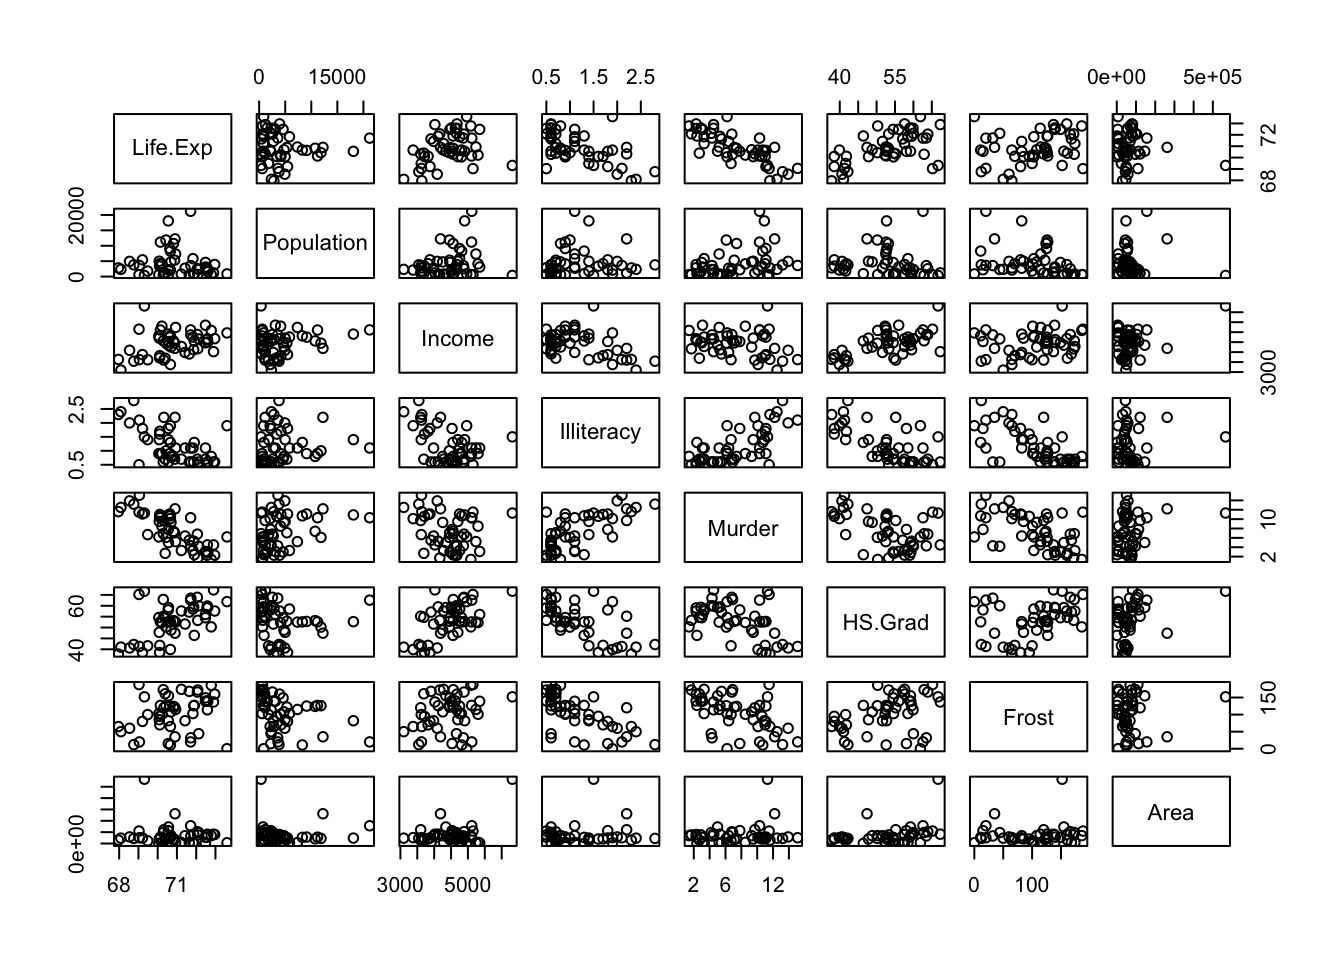
\includegraphics{Statistical_Methods_II_files/figure-latex/unnamed-chunk-131-1.pdf}

I want to add a quadratic effect for HS.Grad rate and for Income. We'll
add it to the data frame and then perform the backward elimination
method starting with the model with all predictors as main effects.

\begin{Shaded}
\begin{Highlighting}[]
\NormalTok{state.data$HS.Grad}\FloatTok{.2} \NormalTok{<-}\StringTok{ }\NormalTok{state.data$HS.Grad ^}\StringTok{ }\DecValTok{2}
\NormalTok{state.data$Income}\FloatTok{.2}  \NormalTok{<-}\StringTok{ }\NormalTok{state.data$Income  ^}\StringTok{ }\DecValTok{2}
\CommentTok{# explicitly define my starting model}
\NormalTok{m1 <-}\StringTok{ }\KeywordTok{lm}\NormalTok{(Life.Exp ~}\StringTok{ }\NormalTok{Population +}\StringTok{ }\NormalTok{Income +}\StringTok{ }\NormalTok{Illiteracy +}\StringTok{ }
\StringTok{                    }\NormalTok{Murder +}\StringTok{ }\NormalTok{HS.Grad +}\StringTok{ }\NormalTok{Frost +}\StringTok{ }\NormalTok{HS.Grad}\FloatTok{.2} \NormalTok{+}\StringTok{ }\NormalTok{Income}\FloatTok{.2}\NormalTok{, }\DataTypeTok{data=}\NormalTok{state.data)}
\CommentTok{#}
\CommentTok{# Define the same model, but using shorthand}
\CommentTok{# The '.' means everything else in the data frame}
\NormalTok{m1 <-}\StringTok{ }\KeywordTok{lm}\NormalTok{( Life.Exp ~}\StringTok{ }\NormalTok{., }\DataTypeTok{data=}\NormalTok{state.data)}
\KeywordTok{summary}\NormalTok{(m1)$coefficients %>%}\StringTok{ }\KeywordTok{round}\NormalTok{(}\DataTypeTok{digits=}\DecValTok{3}\NormalTok{)}
\end{Highlighting}
\end{Shaded}

\begin{verbatim}
##             Estimate Std. Error t value Pr(>|t|)
## (Intercept)   63.413      7.449   8.513    0.000
## Population     0.000      0.000   1.310    0.198
## Income         0.004      0.003   1.605    0.116
## Illiteracy     0.255      0.388   0.656    0.515
## Murder        -0.300      0.049  -6.088    0.000
## HS.Grad       -0.053      0.214  -0.248    0.806
## Frost         -0.004      0.003  -1.374    0.177
## Area           0.000      0.000   0.656    0.516
## HS.Grad.2      0.001      0.002   0.460    0.648
## Income.2       0.000      0.000  -1.618    0.114
\end{verbatim}

The signs make reasonable sense (higher murder rates decrease life
expectancy) but covariates like \texttt{Income} are not significant,
which is surprising. We will first remove the term with the highest
p-value, which is the state's \texttt{HS.Grad}. However, I don't want to
remove the lower-order graduation term and keep the squared-term. So
instead I will remove both of them since they are the highest p-values.
Notice that \texttt{HS.Grad} is correlated with \texttt{Income} and
\texttt{Illiteracy}.

\begin{Shaded}
\begin{Highlighting}[]
\CommentTok{# Remove Graduation Rate from the model from the model}
\NormalTok{m1 <-}\StringTok{ }\KeywordTok{update}\NormalTok{(m1, .~. -}\StringTok{ }\NormalTok{HS.Grad -}\StringTok{ }\NormalTok{HS.Grad}\FloatTok{.2}\NormalTok{)}
\KeywordTok{summary}\NormalTok{(m1)$coefficients %>%}\StringTok{ }\KeywordTok{round}\NormalTok{(}\DataTypeTok{digits=}\DecValTok{3}\NormalTok{)}
\end{Highlighting}
\end{Shaded}

\begin{verbatim}
##             Estimate Std. Error t value Pr(>|t|)
## (Intercept)   62.497      6.395   9.772    0.000
## Population     0.000      0.000   0.838    0.407
## Income         0.005      0.003   1.804    0.078
## Illiteracy    -0.076      0.358  -0.212    0.833
## Murder        -0.308      0.047  -6.573    0.000
## Frost         -0.006      0.003  -1.948    0.058
## Area           0.000      0.000   1.688    0.099
## Income.2       0.000      0.000  -1.750    0.087
\end{verbatim}

\begin{Shaded}
\begin{Highlighting}[]
\CommentTok{# Next remove Illiteracy}
\NormalTok{m1 <-}\StringTok{ }\KeywordTok{update}\NormalTok{(m1, .~. -}\StringTok{ }\NormalTok{Illiteracy)}
\KeywordTok{summary}\NormalTok{(m1)$coefficients %>%}\StringTok{ }\KeywordTok{round}\NormalTok{(}\DataTypeTok{digits=}\DecValTok{3}\NormalTok{)}
\end{Highlighting}
\end{Shaded}

\begin{verbatim}
##             Estimate Std. Error t value Pr(>|t|)
## (Intercept)   61.779      5.367  11.510    0.000
## Population     0.000      0.000   0.860    0.394
## Income         0.005      0.002   2.165    0.036
## Murder        -0.312      0.043  -7.304    0.000
## Frost         -0.006      0.003  -2.261    0.029
## Area           0.000      0.000   1.736    0.090
## Income.2       0.000      0.000  -2.069    0.045
\end{verbatim}

\begin{Shaded}
\begin{Highlighting}[]
\CommentTok{# And Population...}
\NormalTok{m1 <-}\StringTok{ }\KeywordTok{update}\NormalTok{(m1, .~. -}\StringTok{ }\NormalTok{Population)}
\KeywordTok{summary}\NormalTok{(m1)$coefficients %>%}\StringTok{ }\KeywordTok{round}\NormalTok{(}\DataTypeTok{digits=}\DecValTok{3}\NormalTok{)}
\end{Highlighting}
\end{Shaded}

\begin{verbatim}
##             Estimate Std. Error t value Pr(>|t|)
## (Intercept)   59.985      4.931  12.166    0.000
## Income         0.006      0.002   2.702    0.010
## Murder        -0.297      0.039  -7.633    0.000
## Frost         -0.006      0.003  -2.471    0.017
## Area           0.000      0.000   1.746    0.088
## Income.2       0.000      0.000  -2.533    0.015
\end{verbatim}

\begin{Shaded}
\begin{Highlighting}[]
\CommentTok{# Remove Area from the model}
\NormalTok{m1 <-}\StringTok{ }\KeywordTok{update}\NormalTok{(m1, .~. -}\StringTok{ }\NormalTok{Area)}
\KeywordTok{summary}\NormalTok{(m1)$coefficients %>%}\StringTok{ }\KeywordTok{round}\NormalTok{(}\DataTypeTok{digits=}\DecValTok{3}\NormalTok{)}
\end{Highlighting}
\end{Shaded}

\begin{verbatim}
##             Estimate Std. Error t value Pr(>|t|)
## (Intercept)   63.685      4.552  13.990    0.000
## Income         0.004      0.002   2.078    0.043
## Murder        -0.285      0.039  -7.278    0.000
## Frost         -0.006      0.003  -2.235    0.030
## Income.2       0.000      0.000  -1.864    0.069
\end{verbatim}

The removal of \texttt{Income.2} is a tough decision because the p-value
is very close to \(\alpha=0.05\) and might be left in if it makes model
interpretation easier or if the researcher feels a quadratic effect in
income is appropriate (perhaps rich people are too stressed?).

\begin{Shaded}
\begin{Highlighting}[]
\KeywordTok{summary}\NormalTok{(m1)}
\end{Highlighting}
\end{Shaded}

\begin{verbatim}
## 
## Call:
## lm(formula = Life.Exp ~ Income + Murder + Frost + Income.2, data = state.data)
## 
## Residuals:
##      Min       1Q   Median       3Q      Max 
## -1.44396 -0.53231 -0.04994  0.50160  1.51754 
## 
## Coefficients:
##               Estimate Std. Error t value Pr(>|t|)    
## (Intercept)  6.369e+01  4.552e+00  13.990  < 2e-16 ***
## Income       4.017e-03  1.933e-03   2.078   0.0434 *  
## Murder      -2.852e-01  3.918e-02  -7.278 3.95e-09 ***
## Frost       -5.686e-03  2.544e-03  -2.235   0.0304 *  
## Income.2    -3.955e-07  2.121e-07  -1.864   0.0688 .  
## ---
## Signif. codes:  0 '***' 0.001 '**' 0.01 '*' 0.05 '.' 0.1 ' ' 1
## 
## Residual standard error: 0.7619 on 45 degrees of freedom
## Multiple R-squared:  0.7042, Adjusted R-squared:  0.6779 
## F-statistic: 26.78 on 4 and 45 DF,  p-value: 2.112e-11
\end{verbatim}

We are left with a model that adequately explains \texttt{Life.Exp} but
we should be careful to note that just because a covariate was removed
from the model does not imply that it isn't related to the response. For
example, being a high school graduate is highly correlated with not
being illiterate as is \texttt{Income} and thus replacing
\texttt{Illiteracy} shows that illiteracy is associated with lower life
expectancy, but it is not as predictive as \texttt{Income}.

\begin{Shaded}
\begin{Highlighting}[]
\NormalTok{m2 <-}\StringTok{ }\KeywordTok{lm}\NormalTok{(Life.Exp ~}\StringTok{ }\NormalTok{Illiteracy+Murder+Frost, }\DataTypeTok{data=}\NormalTok{state.data)}
\KeywordTok{summary}\NormalTok{(m2)}
\end{Highlighting}
\end{Shaded}

\begin{verbatim}
## 
## Call:
## lm(formula = Life.Exp ~ Illiteracy + Murder + Frost, data = state.data)
## 
## Residuals:
##      Min       1Q   Median       3Q      Max 
## -1.59010 -0.46961  0.00394  0.57060  1.92292 
## 
## Coefficients:
##              Estimate Std. Error t value Pr(>|t|)    
## (Intercept) 74.556717   0.584251 127.611  < 2e-16 ***
## Illiteracy  -0.601761   0.298927  -2.013  0.04998 *  
## Murder      -0.280047   0.043394  -6.454 6.03e-08 ***
## Frost       -0.008691   0.002959  -2.937  0.00517 ** 
## ---
## Signif. codes:  0 '***' 0.001 '**' 0.01 '*' 0.05 '.' 0.1 ' ' 1
## 
## Residual standard error: 0.7911 on 46 degrees of freedom
## Multiple R-squared:  0.6739, Adjusted R-squared:  0.6527 
## F-statistic: 31.69 on 3 and 46 DF,  p-value: 2.915e-11
\end{verbatim}

Notice that the \(R^{2}\) values for both models are quite similar
\(0.7042\) vs \(0.6739\) but the first model with the higher \(R^{2}\)
has one more predictor variable? Which model should I prefer? I can't do
an F-test because these models are not nested.

\section{Criterion Based Procedures}\label{criterion-based-procedures}

\subsection{Information Criterions}\label{information-criterions}

It is often necessary to compare models that are not nested. For
example, I might want to compare \[y=\beta_{0}+\beta_{1}x+\epsilon\] vs
\[y=\beta_{0}+\beta_{2}w+\epsilon\]

This comparison comes about naturally when doing forward model selection
and we are looking for the ``best'' covariate to add to the model first.

Akaike introduced his criterion (which he called ``An Information
Criterion'') as
\[AIC=\underset{\textrm{decreases if RSS decreases}}{\underbrace{-2\,\log L\left(\hat{\boldsymbol{\beta}},\hat{\sigma}|\,\textrm{data}\,\right)}}+\underset{\textrm{increases as p increases}}{\underbrace{2p}}\]
where \(L\left(\hat{\boldsymbol{\beta}}|\,\textrm{data}\,\right)\) is
the likelihood function and \(p\) is the number of elements in the
\(\hat{\boldsymbol{\beta}}\) vector and we regard a lower AIC value as
better. Notice the \(2p\) term is essentially a penalty on adding
addition covariates so to lower the AIC value, a new predictor must
lower the negative log likelihood more than it increases the penalty.

To convince ourselves that the first summand decreases with decreasing
RSS in the standard linear model, we examine the likelihood function
\[\begin{aligned}
f\left(\boldsymbol{y}\,|\,\boldsymbol{\beta},\sigma,\boldsymbol{X}\right)   &=  \frac{1}{\left(2\pi\sigma^{2}\right)^{n/2}}\exp\left[-\frac{1}{2\sigma^{2}}\left(\boldsymbol{y}-\boldsymbol{X}\boldsymbol{\beta}\right)^{T}\left(\boldsymbol{y}-\boldsymbol{X}\boldsymbol{\beta}\right)\right] \\
    &=  L\left(\boldsymbol{\beta},\sigma\,|\,\boldsymbol{y},\boldsymbol{X}\right)
\end{aligned}\] and we could re-write this as \[\begin{aligned}
\log L\left(\hat{\boldsymbol{\beta}},\hat{\sigma}\,|\,\textrm{data}\right)  &=  -\log\left(\left(2\pi\hat{\sigma}^{2}\right)^{n/2}\right)-\frac{1}{2\hat{\sigma}^{2}}\left(\boldsymbol{y}-\boldsymbol{X}\hat{\boldsymbol{\beta}}\right)^{T}\left(\boldsymbol{y}-\boldsymbol{X}\hat{\boldsymbol{\beta}}\right) \\
    &=  -\frac{n}{2}\log\left(2\pi\hat{\sigma}^{2}\right)-\frac{1}{2\hat{\sigma}^{2}}\left(\boldsymbol{y}-\boldsymbol{X}\hat{\boldsymbol{\beta}}\right)^{T}\left(\boldsymbol{y}-\boldsymbol{X}\hat{\boldsymbol{\beta}}\right) \\
    &=  -\frac{1}{2}\left[n\log\left(2\pi\hat{\sigma}^{2}\right)+\frac{1}{\hat{\sigma}^{2}}\left(\boldsymbol{y}-\boldsymbol{X}\hat{\boldsymbol{\beta}}\right)^{T}\left(\boldsymbol{y}-\boldsymbol{X}\hat{\boldsymbol{\beta}}\right)\right] \\
    &=  -\frac{1}{2}\left[+n\log\left(2\pi\right)+n\log\hat{\sigma}^{2}+\frac{1}{\hat{\sigma}^{2}}RSS\right]
\end{aligned}\]

It isn't clear what we should do with the \(n\log\left(2\pi\right)\)
term in the \(\log L()\) function. There are some compelling reasons to
ignore it and just use the second, and there are reasons to use both
terms. Unfortunately, statisticians have not settled on one convention
or the other and different software packages might therefore report
different values for AIC.

As a general rule of thumb, if the difference in AIC values is less than
two then the models are not significantly different, differences between
2 and 4 AIC units are marginally significant and any difference greater
than 4 AIC units is highly significant.

Notice that while this allows us to compare models that are not nested,
it does require that the same data are used to fit both models. Because
I could start out with my data frame including both \(x\) and \(x^{2}\),
(or more generally \(x\) and \(f\left(x\right)\) for some function
\(f()\)) you can regard a transformation of a covariate as ``the same
data''. However, a transformation of a y-variable is not and therefore
we cannot use AIC to compare a models
\texttt{log(y)\ \textasciitilde{}\ x} versus the model
\texttt{y\ \textasciitilde{}\ x}.

Another criterion that might be used is \emph{Bayes Information
Criterion} (BIC) which is

\[BIC=-2\,\log L\left(\hat{\boldsymbol{\beta}},\hat{\sigma}|\,\textrm{data}\,\right)+p\log n\]

and this criterion punishes large models more than AIC does (because
\(\log n>2\) for \(n\ge8\))

The AIC value of a linear model can be found using the AIC() on a lm()
object.

\begin{Shaded}
\begin{Highlighting}[]
\KeywordTok{AIC}\NormalTok{(m1)}
\end{Highlighting}
\end{Shaded}

\begin{verbatim}
## [1] 121.4293
\end{verbatim}

\begin{Shaded}
\begin{Highlighting}[]
\KeywordTok{AIC}\NormalTok{(m2)}
\end{Highlighting}
\end{Shaded}

\begin{verbatim}
## [1] 124.2947
\end{verbatim}

Because the AIC value for the first model is lower, we would prefer the
first model that includes both \texttt{Income} and \texttt{Income.2}
compared to model 2, which was
\texttt{Life.Exp\ \textasciitilde{}\ Illiteracy+Murder+Frost}.

\subsection{\texorpdfstring{Adjusted
\texttt{R-sq}}{Adjusted R-sq}}\label{adjusted-r-sq}

One of the problems with \(R^{2}\) is that it makes no adjustment for
how many parameters in the model. Recall that \(R^{2}\) was defined as
\[R^{2}=\frac{RSS_{S}-RSS_{C}}{RSS_{S}}=1-\frac{RSS_{C}}{RSS_{S}}\]
where the simple model was the intercept only model. We can create an
\(R_{adj}^{2}\) statistic that attempts to add a penalty for having too
many parameters by defining
\[R_{adj}^{2}=1-\frac{RSS_{C}/\left(n-p\right)}{RSS_{S}/\left(n-1\right)}\]
With this adjusted definition, adding a variable to the model that has
no predictive power will decrease \(R_{adj}^{2}\).

\subsection{Example}\label{example}

Returning to the life expectancy data, we could start with a simple
model add covariates to the model that have the lowest AIC values. R
makes this easy with the function add1() which will take a linear model
(which includes the data frame that originally defined it) and will
sequentially add all of the possible terms that are not currently in the
model and report the AIC values for each model.

\begin{Shaded}
\begin{Highlighting}[]
\CommentTok{# Define the biggest model I wish to consider}
\NormalTok{biggest <-}\StringTok{ }\NormalTok{Life.Exp ~}\StringTok{ }\NormalTok{Population +}\StringTok{ }\NormalTok{Income +}\StringTok{ }\NormalTok{Illiteracy +}\StringTok{ }\NormalTok{Murder +}\StringTok{ }
\StringTok{                      }\NormalTok{HS.Grad +}\StringTok{ }\NormalTok{Frost +}\StringTok{ }\NormalTok{Area +}\StringTok{ }\NormalTok{HS.Grad}\FloatTok{.2} \NormalTok{+}\StringTok{ }\NormalTok{Income}\FloatTok{.2}

\CommentTok{# Define the model I wish to start with}
\NormalTok{m <-}\StringTok{ }\KeywordTok{lm}\NormalTok{(Life.Exp ~}\StringTok{ }\DecValTok{1}\NormalTok{, }\DataTypeTok{data=}\NormalTok{state.data)}

\KeywordTok{add1}\NormalTok{(m, }\DataTypeTok{scope=}\NormalTok{biggest)  }\CommentTok{# what is the best addition to make?}
\end{Highlighting}
\end{Shaded}

\begin{verbatim}
## Single term additions
## 
## Model:
## Life.Exp ~ 1
##            Df Sum of Sq    RSS     AIC
## <none>                  88.299  30.435
## Population  1     0.409 87.890  32.203
## Income      1    10.223 78.076  26.283
## Illiteracy  1    30.578 57.721  11.179
## Murder      1    53.838 34.461 -14.609
## HS.Grad     1    29.931 58.368  11.737
## Frost       1     6.064 82.235  28.878
## Area        1     1.017 87.282  31.856
## HS.Grad.2   1    27.414 60.885  13.848
## Income.2    1     7.464 80.835  28.020
\end{verbatim}

Clearly the additiona of \texttt{Murder} to the model results in the
lowest AIC value, so we will add \texttt{Murder} to the model. Notice
the \texttt{\textless{}none\textgreater{}} row corresponds to the model
m which we started with and it has a \texttt{RSS=88.299}. For each model
considered, R will calculate the \texttt{RSS\_\{C\}} for the new model
and will calculate the difference between the starting model and the
more complicated model and display this in the Sum of Squares column.

\begin{Shaded}
\begin{Highlighting}[]
\NormalTok{m <-}\StringTok{ }\KeywordTok{update}\NormalTok{(m, . ~}\StringTok{ }\NormalTok{. +}\StringTok{ }\NormalTok{Murder)  }\CommentTok{# add murder to the model}
\KeywordTok{add1}\NormalTok{(m, }\DataTypeTok{scope=}\NormalTok{biggest)          }\CommentTok{# what should I add next?}
\end{Highlighting}
\end{Shaded}

\begin{verbatim}
## Single term additions
## 
## Model:
## Life.Exp ~ Murder
##            Df Sum of Sq    RSS     AIC
## <none>                  34.461 -14.609
## Population  1    4.0161 30.445 -18.805
## Income      1    2.4047 32.057 -16.226
## Illiteracy  1    0.2732 34.188 -13.007
## HS.Grad     1    4.6910 29.770 -19.925
## Frost       1    3.1346 31.327 -17.378
## Area        1    0.4697 33.992 -13.295
## HS.Grad.2   1    4.4396 30.022 -19.505
## Income.2    1    1.8972 32.564 -15.441
\end{verbatim}

There is a companion function to \texttt{add1()} that finds the best
term to drop. It is conveniently named \texttt{drop1()} but here the
\texttt{scope} parameter defines the smallest model to be considered.

It would be nice if all of this work was automated. Again, R makes our
life easy and the function \texttt{step()} does exactly this. The set of
models searched is determined by the scope argument which can be a
\emph{list} of two formulas with components upper and lower or it can be
a single formula, or it can be blank. The right-hand-side of its lower
component defines the smallest model to be considered and the
right-hand-side of the upper component defines the largest model to be
considered. If \texttt{scope} is a single formula, it specifies the
upper component, and the lower model taken to be the intercept-only
model. If scope is missing, the initial model is used as the upper
model.

\begin{Shaded}
\begin{Highlighting}[]
\NormalTok{smallest <-}\StringTok{ }\NormalTok{Life.Exp ~}\StringTok{ }\DecValTok{1}
\NormalTok{biggest <-}\StringTok{ }\NormalTok{Life.Exp ~}\StringTok{ }\NormalTok{Population +}\StringTok{ }\NormalTok{Income +}\StringTok{ }\NormalTok{Illiteracy +}\StringTok{ }
\StringTok{                      }\NormalTok{Murder +}\StringTok{ }\NormalTok{HS.Grad +}\StringTok{ }\NormalTok{Frost +}\StringTok{ }\NormalTok{Area +}\StringTok{ }\NormalTok{HS.Grad}\FloatTok{.2} \NormalTok{+}\StringTok{ }\NormalTok{Income}\FloatTok{.2}
\NormalTok{m <-}\StringTok{ }\KeywordTok{lm}\NormalTok{(Life.Exp ~}\StringTok{ }\NormalTok{Income, }\DataTypeTok{data=}\NormalTok{state.data)}
\KeywordTok{step}\NormalTok{(m, }\DataTypeTok{scope=}\KeywordTok{list}\NormalTok{(}\DataTypeTok{lower=}\NormalTok{smallest, }\DataTypeTok{upper=}\NormalTok{biggest))}
\end{Highlighting}
\end{Shaded}

\begin{verbatim}
## Start:  AIC=26.28
## Life.Exp ~ Income
## 
##              Df Sum of Sq    RSS     AIC
## + Murder      1    46.020 32.057 -16.226
## + Illiteracy  1    21.109 56.968  12.523
## + HS.Grad     1    19.770 58.306  13.684
## + Income.2    1    19.062 59.015  14.288
## + HS.Grad.2   1    17.193 60.884  15.847
## + Area        1     5.426 72.650  24.682
## + Frost       1     3.188 74.889  26.199
## <none>                    78.076  26.283
## + Population  1     1.781 76.295  27.130
## - Income      1    10.223 88.299  30.435
## 
## Step:  AIC=-16.23
## Life.Exp ~ Income + Murder
## 
##              Df Sum of Sq    RSS     AIC
## + Frost       1     3.918 28.138 -20.745
## + Income.2    1     3.036 29.021 -19.200
## + Population  1     2.552 29.504 -18.374
## + HS.Grad     1     2.388 29.668 -18.097
## + HS.Grad.2   1     2.199 29.857 -17.780
## <none>                    32.057 -16.226
## - Income      1     2.405 34.461 -14.609
## + Illiteracy  1     0.011 32.046 -14.242
## + Area        1     0.000 32.057 -14.226
## - Murder      1    46.020 78.076  26.283
## 
## Step:  AIC=-20.74
## Life.Exp ~ Income + Murder + Frost
## 
##              Df Sum of Sq    RSS     AIC
## + HS.Grad     1     2.949 25.189 -24.280
## + HS.Grad.2   1     2.764 25.375 -23.914
## + Income.2    1     2.017 26.121 -22.465
## + Population  1     1.341 26.797 -21.187
## <none>                    28.138 -20.745
## + Illiteracy  1     0.950 27.189 -20.461
## + Area        1     0.147 27.991 -19.007
## - Income      1     3.188 31.327 -17.378
## - Frost       1     3.918 32.057 -16.226
## - Murder      1    46.750 74.889  26.199
## 
## Step:  AIC=-24.28
## Life.Exp ~ Income + Murder + Frost + HS.Grad
## 
##              Df Sum of Sq    RSS     AIC
## + Population  1     1.887 23.302 -26.174
## + Income.2    1     1.864 23.326 -26.124
## - Income      1     0.182 25.372 -25.920
## <none>                    25.189 -24.280
## + HS.Grad.2   1     0.218 24.972 -22.714
## + Illiteracy  1     0.131 25.058 -22.541
## + Area        1     0.058 25.131 -22.395
## - HS.Grad     1     2.949 28.138 -20.745
## - Frost       1     4.479 29.668 -18.097
## - Murder      1    32.877 58.067  15.478
## 
## Step:  AIC=-26.17
## Life.Exp ~ Income + Murder + Frost + HS.Grad + Population
## 
##              Df Sum of Sq    RSS     AIC
## - Income      1     0.006 23.308 -28.161
## <none>                    23.302 -26.174
## + Income.2    1     0.790 22.512 -25.899
## - Population  1     1.887 25.189 -24.280
## + HS.Grad.2   1     0.006 23.296 -24.187
## + Illiteracy  1     0.004 23.298 -24.182
## + Area        1     0.000 23.302 -24.174
## - Frost       1     3.037 26.339 -22.048
## - HS.Grad     1     3.495 26.797 -21.187
## - Murder      1    34.739 58.041  17.456
## 
## Step:  AIC=-28.16
## Life.Exp ~ Murder + Frost + HS.Grad + Population
## 
##              Df Sum of Sq    RSS     AIC
## <none>                    23.308 -28.161
## + Income.2    1     0.031 23.277 -26.229
## + HS.Grad.2   1     0.007 23.301 -26.177
## + Income      1     0.006 23.302 -26.174
## + Illiteracy  1     0.004 23.304 -26.170
## + Area        1     0.001 23.307 -26.163
## - Population  1     2.064 25.372 -25.920
## - Frost       1     3.122 26.430 -23.877
## - HS.Grad     1     5.112 28.420 -20.246
## - Murder      1    34.816 58.124  15.528
\end{verbatim}

\begin{verbatim}
## 
## Call:
## lm(formula = Life.Exp ~ Murder + Frost + HS.Grad + Population, 
##     data = state.data)
## 
## Coefficients:
## (Intercept)       Murder        Frost      HS.Grad   Population  
##   7.103e+01   -3.001e-01   -5.943e-03    4.658e-02    5.014e-05
\end{verbatim}

Notice that our model selected by \texttt{step()} is not the same model
we obtained when we started with the biggest model and removed things
based on p-values.

The log-likelihood is only defined up to an additive constant, and there
are different conventional constants used. This is more annoying than
anything because all we care about for model selection is the difference
between AIC values of two models and the additive constant cancels. The
only time it matters is when you have two different ways of extracting
the AIC values. Recall the model we fit using the top-down approach was

\begin{Shaded}
\begin{Highlighting}[]
\CommentTok{# m1 was}
\NormalTok{m1 <-}\StringTok{ }\KeywordTok{lm}\NormalTok{(Life.Exp ~}\StringTok{ }\NormalTok{Income +}\StringTok{ }\NormalTok{Murder +}\StringTok{ }\NormalTok{Frost +}\StringTok{ }\NormalTok{Income}\FloatTok{.2}\NormalTok{, }\DataTypeTok{data =} \NormalTok{state.data)}
\KeywordTok{AIC}\NormalTok{(m1)}
\end{Highlighting}
\end{Shaded}

\begin{verbatim}
## [1] 121.4293
\end{verbatim}

and the model selected by the stepwise algorithm was

\begin{Shaded}
\begin{Highlighting}[]
\NormalTok{m3 <-}\StringTok{ }\KeywordTok{lm}\NormalTok{(Life.Exp ~}\StringTok{ }\NormalTok{Murder +}\StringTok{ }\NormalTok{Frost +}\StringTok{ }\NormalTok{HS.Grad +}\StringTok{ }\NormalTok{Population, }\DataTypeTok{data =} \NormalTok{state.data)}
\KeywordTok{AIC}\NormalTok{(m3)}
\end{Highlighting}
\end{Shaded}

\begin{verbatim}
## [1] 115.7326
\end{verbatim}

Because \texttt{step()} and \texttt{AIC()} are following different
conventions the absolute value of the AICs are different, but the
difference between the two is constant no matter which function we use.

First we calculate the difference using the AIC() function:

\begin{Shaded}
\begin{Highlighting}[]
\KeywordTok{AIC}\NormalTok{(m1) -}\StringTok{ }\KeywordTok{AIC}\NormalTok{(m3)}
\end{Highlighting}
\end{Shaded}

\begin{verbatim}
## [1] 5.696681
\end{verbatim}

and next we use \texttt{add1()} on both models to see what the AIC
values for each.

\begin{Shaded}
\begin{Highlighting}[]
\KeywordTok{add1}\NormalTok{(m1, }\DataTypeTok{scope=}\NormalTok{biggest)}
\end{Highlighting}
\end{Shaded}

\begin{verbatim}
## Single term additions
## 
## Model:
## Life.Exp ~ Income + Murder + Frost + Income.2
##            Df Sum of Sq    RSS     AIC
## <none>                  26.121 -22.465
## Population  1   0.42412 25.697 -21.283
## Illiteracy  1   0.10097 26.020 -20.658
## HS.Grad     1   2.79527 23.326 -26.124
## Area        1   1.69309 24.428 -23.815
## HS.Grad.2   1   2.79698 23.324 -26.127
\end{verbatim}

\begin{Shaded}
\begin{Highlighting}[]
\KeywordTok{add1}\NormalTok{(m3, }\DataTypeTok{scope=}\NormalTok{biggest)}
\end{Highlighting}
\end{Shaded}

\begin{verbatim}
## Single term additions
## 
## Model:
## Life.Exp ~ Murder + Frost + HS.Grad + Population
##            Df Sum of Sq    RSS     AIC
## <none>                  23.308 -28.161
## Income      1 0.0060582 23.302 -26.174
## Illiteracy  1 0.0039221 23.304 -26.170
## Area        1 0.0007900 23.307 -26.163
## HS.Grad.2   1 0.0073439 23.301 -26.177
## Income.2    1 0.0314248 23.277 -26.229
\end{verbatim}

Using these results, we can calculate the difference in AIC values to be
the same as we calculated before \[\begin{aligned}
-22.465--28.161 &=  -22.465+28.161 \\
    &=  5.696
    \end{aligned}\]

\section{Exercises}\label{exercises-6}

\begin{enumerate}
\def\labelenumi{\arabic{enumi}.}
\item
  Consider the \texttt{prostate} data from the \texttt{faraway} package.
  The variable \texttt{lpsa} is a measurement of a prostate specific
  antigen which higher levels are indicative of prostate cancer. Use
  \texttt{lpsa} as the response and all the other variables as
  predictors (no interactions). Determine the ``best'' model using:

  \begin{enumerate}
  \def\labelenumii{\alph{enumii}.}
  \item
    Backward elimination using the analysis of variance F-statistic as
    the criteria.
  \item
    Forward selection using AIC as the criteria.
  \end{enumerate}
\item
  Again from the \texttt{faraway} package, use the \texttt{divusa} which
  has diviorce rates for each year from 1920-1996 along with other
  population information for each year. Use \texttt{divorce} as the
  response variable and all other variables as the predictors.

  \begin{enumerate}
  \def\labelenumii{\alph{enumii}.}
  \item
    Determine the best model using stepwise selection starting from the
    intercept only model and the most complex model being all main
    effects (no interactions). Use the F-statistic to determine
    significance. Note: add1(), drop1(), and step() allow an option of
    test=`F' to use an F-test instead of AIC.
  \item
    Following the stepwise selection, comment on the relationship
    between p-values used and the AIC difference observed. Do the AIC
    rules of thumb match the p-value interpretation?
  \end{enumerate}
\end{enumerate}

\chapter{One way ANOVA}\label{one-way-anova}

\begin{Shaded}
\begin{Highlighting}[]
\CommentTok{# Load the libraries I'll use}
\KeywordTok{library}\NormalTok{(faraway)}
\KeywordTok{library}\NormalTok{(ggplot2)}
\KeywordTok{library}\NormalTok{(dplyr)}
\KeywordTok{library}\NormalTok{(multcompView)}
\end{Highlighting}
\end{Shaded}

Given a categorical covariate (which I will call a factor) with \(I\)
levels, we are interested in fitting the model
\[y_{ij}=\mu+\tau_{i}+\epsilon_{ij}\] where
\(\epsilon_{ij}\stackrel{iid}{\sim}N\left(0,\sigma^{2}\right)\), \(\mu\)
is the overall mean, and \(\tau_{i}\) are the offset of factor level
\(i\) from \(\mu\). Unfortunately this model is not identifiable because
I could add a constant (say \(5\)) to \(\mu\) and subtract that same
constant from each of the \(\tau_{i}\) values and the group mean
\(\mu+\tau_{i}\) would not change. There are two easy restrictions we
could make to make the model identifiable:

\begin{enumerate}
\def\labelenumi{\arabic{enumi}.}
\item
  Set \(\mu=0\). In this case, \(\tau_{i}\) represents the expected
  value of an observation in group level \(i\). We call this the ``cell
  means'' representation.
\item
  Set \(\tau_{1}=0\). Then \(\mu\) represents the expected value of
  treatment \(1\), and the \(\tau_{i}\) values will represent the
  offsets from group 1. The group or level that we set to be zero is
  then referred to as the reference group. We can call this the ``offset
  from reference'' model.
\end{enumerate}

We will be interested in testing the null and alternative hypotheses
\[\begin{aligned}
H_{0}:\;\;y_{ij}    &=  \mu+\epsilon_{ij}              \\
H_{a}:\;\;y_{ij}    =   \mu+\alpha_{i}+\epsilon_{ij}
\end{aligned}\]

\section{An Example}\label{an-example}

We look at a dataset that comes from the study of blood coagulation
times: 24 animals were randomly assigned to four different diets and the
samples were taken in a random order. The diets are denoted as
\(A\),\(B\),\(C\),and \(D\) and the response of interest is the amount
of time it takes for the blood to coagulate.

\begin{Shaded}
\begin{Highlighting}[]
\KeywordTok{data}\NormalTok{(coagulation)}
\KeywordTok{ggplot}\NormalTok{(coagulation, }\KeywordTok{aes}\NormalTok{(}\DataTypeTok{x=}\NormalTok{diet, }\DataTypeTok{y=}\NormalTok{coag)) +}\StringTok{ }
\StringTok{    }\KeywordTok{geom_boxplot}\NormalTok{() +}
\StringTok{    }\KeywordTok{labs}\NormalTok{( }\DataTypeTok{x=}\StringTok{'Diet'}\NormalTok{, }\DataTypeTok{y=}\StringTok{'Coagulation Time'} \NormalTok{)}
\end{Highlighting}
\end{Shaded}

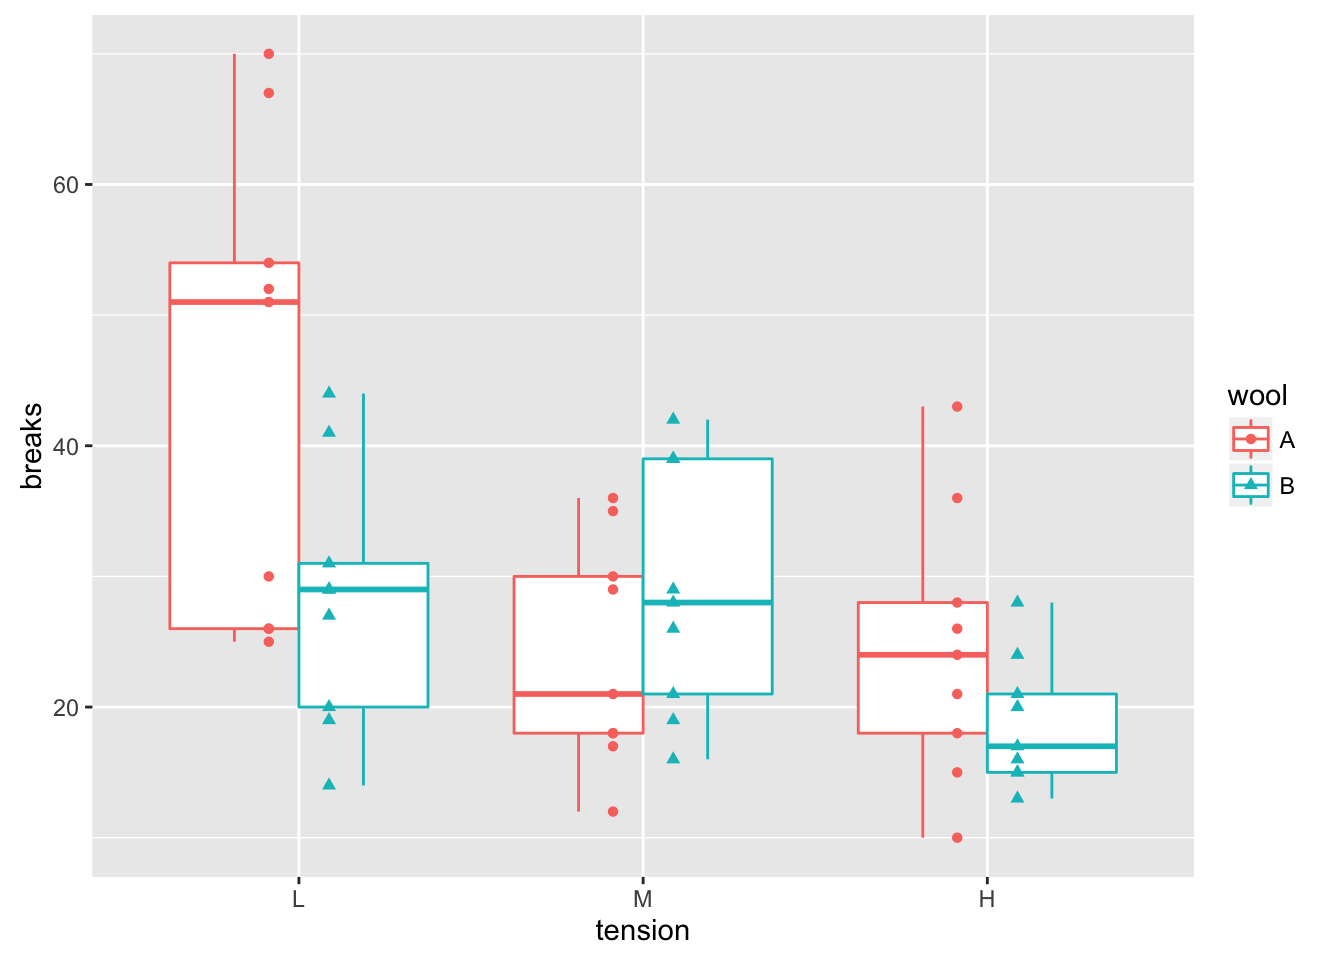
\includegraphics{Statistical_Methods_II_files/figure-latex/unnamed-chunk-149-1.pdf}

Just by looking at the graph, we expect to see that diets \(A\) and
\(D\) are similar while \(B\) and \(C\) are different from \(A\) and
\(D\) and possibly from each other, too. We first fit the offset model.

\begin{Shaded}
\begin{Highlighting}[]
\NormalTok{m <-}\StringTok{ }\KeywordTok{lm}\NormalTok{(coag ~}\StringTok{ }\NormalTok{diet, }\DataTypeTok{data=}\NormalTok{coagulation)}
\KeywordTok{summary}\NormalTok{(m)}
\end{Highlighting}
\end{Shaded}

\begin{verbatim}
## 
## Call:
## lm(formula = coag ~ diet, data = coagulation)
## 
## Residuals:
##    Min     1Q Median     3Q    Max 
##  -5.00  -1.25   0.00   1.25   5.00 
## 
## Coefficients:
##              Estimate Std. Error t value Pr(>|t|)    
## (Intercept) 6.100e+01  1.183e+00  51.554  < 2e-16 ***
## dietB       5.000e+00  1.528e+00   3.273 0.003803 ** 
## dietC       7.000e+00  1.528e+00   4.583 0.000181 ***
## dietD       2.991e-15  1.449e+00   0.000 1.000000    
## ---
## Signif. codes:  0 '***' 0.001 '**' 0.01 '*' 0.05 '.' 0.1 ' ' 1
## 
## Residual standard error: 2.366 on 20 degrees of freedom
## Multiple R-squared:  0.6706, Adjusted R-squared:  0.6212 
## F-statistic: 13.57 on 3 and 20 DF,  p-value: 4.658e-05
\end{verbatim}

Notice that diet \(A\) is the reference level and it has a mean of
\(61\). Diet \(B\) has an offset from \(A\) of \(5\), etc. From the very
small F-statistic, we conclude that simple model
\[y_{ij}=\mu+\epsilon_{ij}\] is not sufficient to describe the data.

\section{Degrees of Freedom}\label{degrees-of-freedom}

Throughout the previous example, the degrees of freedom that are
reported keeps changed depending on what models we are comparing. The
simple model we are considering is \[y_{ij}\sim\mu+\epsilon_{ij}\] which
has 1 parameter that defines the expected value versus
\[y_{ij}\sim\mu+\tau_{i}+\epsilon_{ij}\] where there really are only
\(4\) parameters that define the expected value because \(\tau_{1}=0\).
In general, the larger model is only adding \(I-1\) terms to the model
where \(I\) is the number of levels of the factor of interest.

\section{Diagnostics}\label{diagnostics}

It is still important to check the diagnostics plots, but certain
diagnostic plots will be useless. In particular, we need to be concerned
about constant variance among the groups and normality of the residuals.

\begin{Shaded}
\begin{Highlighting}[]
\KeywordTok{library}\NormalTok{(ggfortify)}
\NormalTok{m <-}\StringTok{ }\KeywordTok{lm}\NormalTok{(coag ~}\StringTok{ }\NormalTok{diet, }\DataTypeTok{data=}\NormalTok{coagulation)}
\KeywordTok{autoplot}\NormalTok{(m, }\DataTypeTok{which=}\DecValTok{2}\NormalTok{)  }\CommentTok{#  QQ plot}
\end{Highlighting}
\end{Shaded}

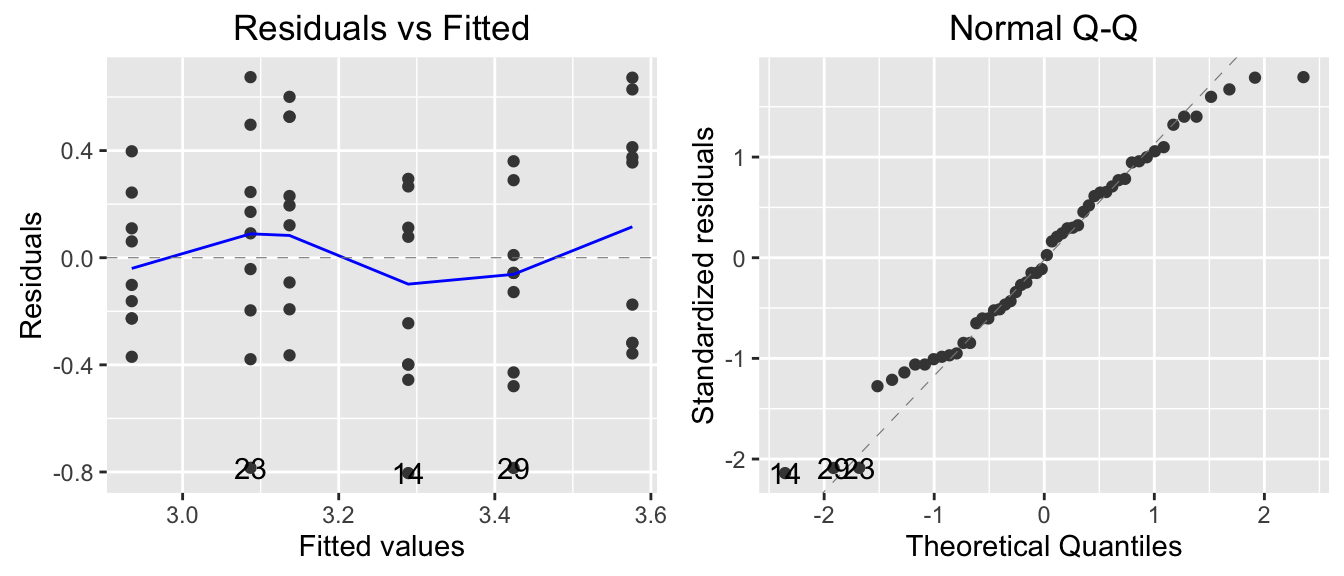
\includegraphics{Statistical_Methods_II_files/figure-latex/unnamed-chunk-151-1.pdf}

The residual plots however, might need a little bit of extra work,
because there are only four possible predicted values (actually \(3\)
because group \(A\) and \(D\) have the same predicted values). Note that
we actually have \(n=24\) observations, but I can only see 16 of them.

\begin{Shaded}
\begin{Highlighting}[]
\KeywordTok{plot}\NormalTok{(m, }\DataTypeTok{which=}\DecValTok{1}\NormalTok{)  }\CommentTok{#  Residals vs fitted}
\end{Highlighting}
\end{Shaded}

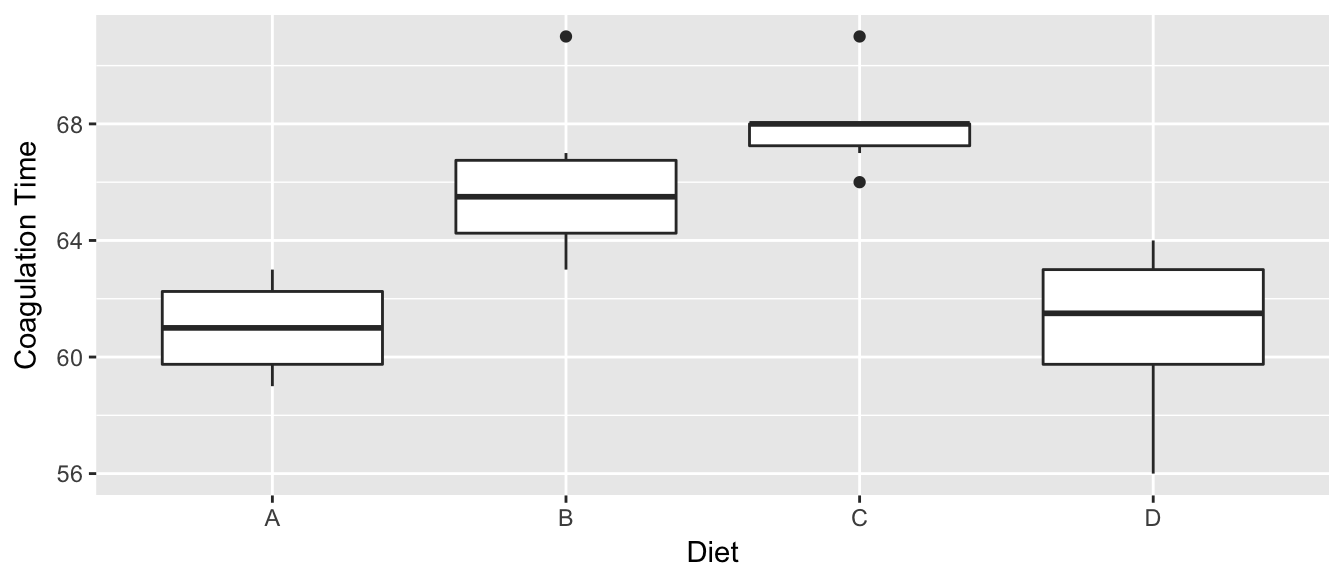
\includegraphics{Statistical_Methods_II_files/figure-latex/unnamed-chunk-152-1.pdf}

To remedy this, we will plot the residuals vs fitted by hand, and add a
little bit of random noise to the fitted value, just so that we don't
have points stack up on top of each other. Lets also add a different
shape for each diet.

\begin{Shaded}
\begin{Highlighting}[]
\NormalTok{coagulation$fitted <-}\StringTok{ }\KeywordTok{predict}\NormalTok{(m)}
\NormalTok{coagulation$resid <-}\StringTok{ }\KeywordTok{resid}\NormalTok{(m)}
\KeywordTok{ggplot}\NormalTok{(coagulation, }\KeywordTok{aes}\NormalTok{(}\DataTypeTok{x=}\NormalTok{fitted, }\DataTypeTok{y=}\NormalTok{resid, }\DataTypeTok{shape=}\NormalTok{diet, }\DataTypeTok{color=}\NormalTok{diet)) +}
\StringTok{  }\KeywordTok{geom_point}\NormalTok{(}\DataTypeTok{position=}\KeywordTok{position_jitter}\NormalTok{(}\DataTypeTok{w=}\FloatTok{0.3}\NormalTok{, }\DataTypeTok{h=}\DecValTok{0}\NormalTok{))}
\end{Highlighting}
\end{Shaded}

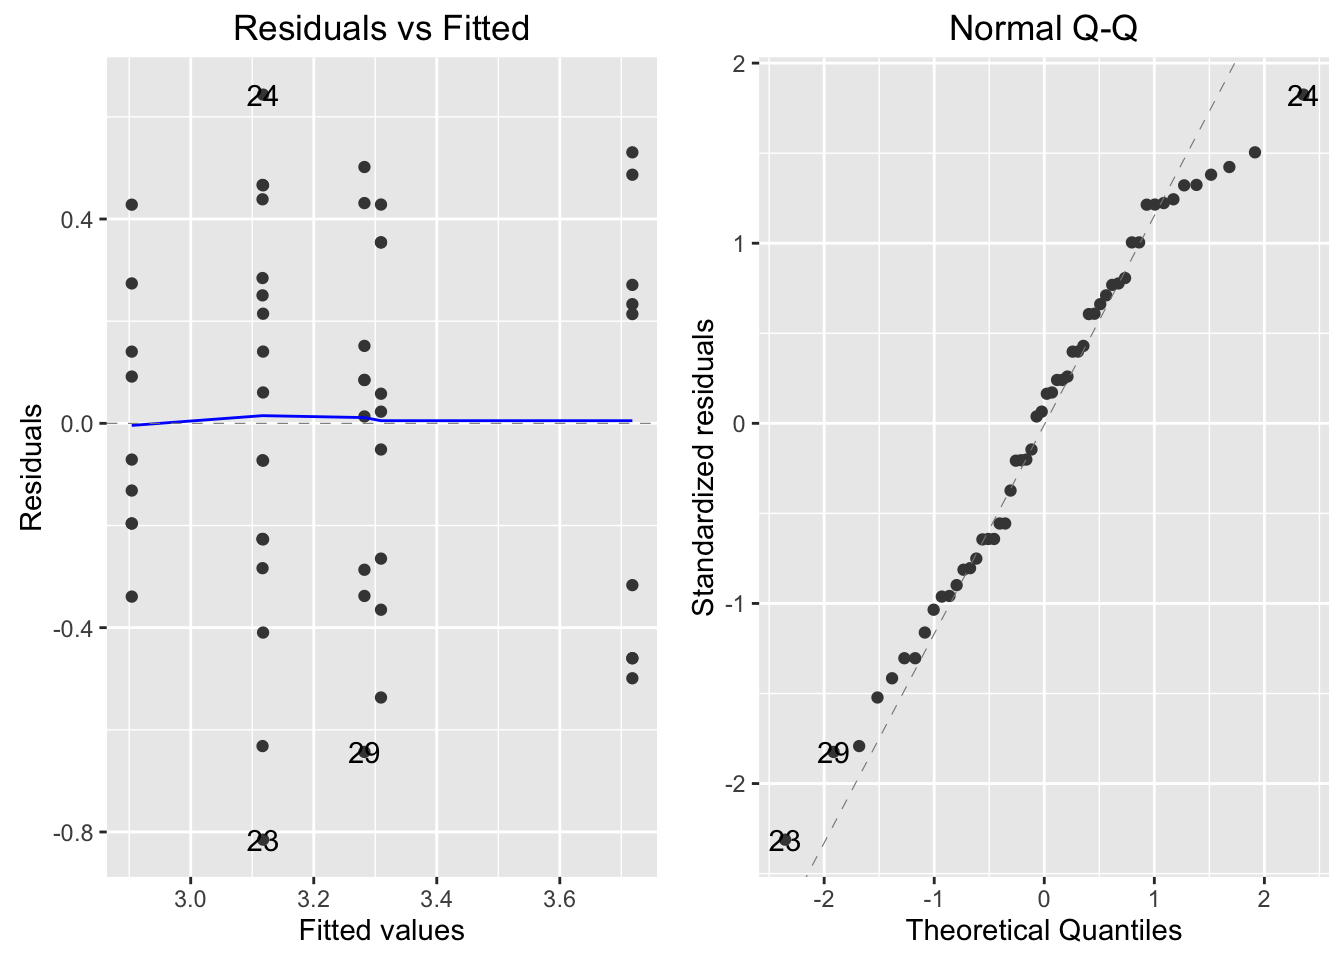
\includegraphics{Statistical_Methods_II_files/figure-latex/unnamed-chunk-153-1.pdf}

\section{Pairwise Comparisons}\label{pairwise-comparisons}

After detecting differences in the factor levels, we are often
interested in which factor levels are different from which. Often we are
interested in comparing the mean of level \(i\) with the mean of level
\(j\). As usual we let the vector of parameter estimates be
\(\hat{\boldsymbol{\beta}}\) then the contrast of interested can be
written as
\[\boldsymbol{c}^{T}\hat{\boldsymbol{\beta}}\pm t_{n-p}^{1-\alpha/2}\;\hat{\sigma}\sqrt{\boldsymbol{c}^{T}\left(\boldsymbol{X}^{T}\boldsymbol{X}\right)^{-1}\boldsymbol{c}}\]
for some vector \(\boldsymbol{c}\).

Unfortunately this interval does not take into account the multiple
comparisons issue (i.e.~we are making \(I(I-1)/2\) contrasts if our
factor has \(I\) levels). To account for this, we will not use a
quantile from a t-distribution, but from Tukey's studentized range
distribution \(q_{n,n-I}\) divided by \(\sqrt{2}\). The intervals we
will use are:
\[\boldsymbol{c}^{T}\hat{\boldsymbol{\beta}}\pm\frac{q_{n,n-I}^{1-\alpha/2}}{\sqrt{2}}\;\hat{\sigma}\sqrt{\boldsymbol{c}^{T}\left(\boldsymbol{X}^{T}\boldsymbol{X}\right)^{-1}\boldsymbol{c}}\]

There are several ways to make R calculate this interval (See the
contrasts chapter for a more general treatment of this.), but the
easiest is to use \texttt{TukeyHSD()}. This function will calculate all
of these pairwise intervals using the above formula, which is commonly
known as Tukey's Honestly Significant Differences. This function expects
to receive output from the aov() function. The aov() is similar to lm()
but does not accept continuous covariates in the model. Because it is
possible to convert a \texttt{lm} output object to an \texttt{aov}
object, I typically will do the following

\begin{Shaded}
\begin{Highlighting}[]
\NormalTok{m <-}\StringTok{ }\KeywordTok{lm}\NormalTok{(coag ~}\StringTok{ }\NormalTok{diet, }\DataTypeTok{data=}\NormalTok{coagulation)   }\CommentTok{# use the lm() function as usual}
\NormalTok{Pvalues <-}\StringTok{ }\KeywordTok{TukeyHSD}\NormalTok{( }\KeywordTok{aov}\NormalTok{(m), }\DataTypeTok{level=}\NormalTok{.}\DecValTok{90} \NormalTok{) }\CommentTok{# convert to the format that TukeyHSD likes...}
\NormalTok{Pvalues}
\end{Highlighting}
\end{Shaded}

\begin{verbatim}
##   Tukey multiple comparisons of means
##     95% family-wise confidence level
## 
## Fit: aov(formula = m)
## 
## $diet
##     diff         lwr       upr     p adj
## B-A    5   0.7245544  9.275446 0.0183283
## C-A    7   2.7245544 11.275446 0.0009577
## D-A    0  -4.0560438  4.056044 1.0000000
## C-B    2  -1.8240748  5.824075 0.4766005
## D-B   -5  -8.5770944 -1.422906 0.0044114
## D-C   -7 -10.5770944 -3.422906 0.0001268
\end{verbatim}

Here we see that diets \(A\) and \(D\) are similar to each other, but
different than \(B\) and \(C\) and that \(B\) and \(C\) are not
statistically different from each other at the \(0.10\) level.

\subsection{Presentation of Results}\label{presentation-of-results}

The display of \texttt{TukeyHSD} is pretty annoying and often I want to
turn the vector of adjusted p-values into a matrix of p-values. We want
a matrix that is \(p \times p\).

\begin{Shaded}
\begin{Highlighting}[]
\CommentTok{# Convert to a matrix of adjusted p-values}
\NormalTok{Pmatrix <-}\StringTok{ }\KeywordTok{vec2mat}\NormalTok{( Pvalues$diet[, }\StringTok{'p adj'}\NormalTok{] )}
\NormalTok{Pmatrix}
\end{Highlighting}
\end{Shaded}

\begin{verbatim}
##             B            C            D            A
## B 1.000000000 0.4766005178 0.0044113688 0.0183282757
## C 0.476600518 1.0000000000 0.0001267866 0.0009576856
## D 0.004411369 0.0001267866 1.0000000000 1.0000000000
## A 0.018328276 0.0009576856 1.0000000000 1.0000000000
\end{verbatim}

From this matrix of adjusted p-values, there are many functions that
will be helpful. One very common thing is to use a lettering scheme that
indicates which groups are different. So if two groups share a letter,
they are not significantly different.

\begin{Shaded}
\begin{Highlighting}[]
\KeywordTok{multcompLetters}\NormalTok{(Pmatrix)}
\end{Highlighting}
\end{Shaded}

\begin{verbatim}
##   B   C   D   A 
## "a" "a" "b" "b"
\end{verbatim}

To make our lives easier while making graphs, we \emph{really} want to
be able to add these back into our original data frame. Unfortunately
the \texttt{multcompView} package that does this doesn't really make it
easy to do this. So I wrote us a little function that will suffice:

\begin{Shaded}
\begin{Highlighting}[]
\CommentTok{#' Create a data frame with significant groupings }
\CommentTok{#'}
\CommentTok{#' This function runs TukeyHSD on the input model and then creates a data frame}
\CommentTok{#' with a column for the factor and a second for the Significance Group}
\CommentTok{#' }
\CommentTok{#' @param model The output of a lm() or aov() call that can be coerced to an aov object.}
\CommentTok{#' @param variable The variable of interest.}
\CommentTok{#' @output A data frame with a column for factor and another for the signicance group.}
\NormalTok{make_TukeyHSD_letters <-}\StringTok{ }\NormalTok{function(model, variable)\{ }
  \NormalTok{Tukey <-}\StringTok{ }\KeywordTok{TukeyHSD}\NormalTok{(}\KeywordTok{aov}\NormalTok{(model))[[variable]]}
  \NormalTok{temp <-}\StringTok{ }\NormalTok{Tukey[,}\StringTok{'p adj'}\NormalTok{] %>%}
\StringTok{    }\KeywordTok{vec2mat}\NormalTok{() %>%}
\StringTok{    }\KeywordTok{multcompLetters}\NormalTok{()}
  \NormalTok{out <-}\StringTok{ }\KeywordTok{data.frame}\NormalTok{(}\DataTypeTok{group =} \KeywordTok{names}\NormalTok{(temp$Letters), }\DataTypeTok{SigGroup=}\NormalTok{temp$Letters)}
  \KeywordTok{colnames}\NormalTok{(out)[}\DecValTok{1}\NormalTok{] <-}\StringTok{ }\NormalTok{variable}
  \NormalTok{out}
\NormalTok{\}  }
\end{Highlighting}
\end{Shaded}

Now that the function is defined, we can happily use it.

\begin{Shaded}
\begin{Highlighting}[]
\KeywordTok{make_TukeyHSD_letters}\NormalTok{(m, }\StringTok{'diet'}\NormalTok{) }
\end{Highlighting}
\end{Shaded}

\begin{verbatim}
##   diet SigGroup
## B    B        a
## C    C        a
## D    D        b
## A    A        b
\end{verbatim}

This is useful, but it will be more useful when I merge this small data
frame with the original data and then each observation will have an
associated significance group.

\begin{Shaded}
\begin{Highlighting}[]
\NormalTok{coagulation <-}\StringTok{ }\NormalTok{coagulation %>%}
\StringTok{  }\KeywordTok{left_join}\NormalTok{( }\KeywordTok{make_TukeyHSD_letters}\NormalTok{(m, }\StringTok{'diet'}\NormalTok{) )}
\end{Highlighting}
\end{Shaded}

\begin{verbatim}
## Joining, by = "diet"
\end{verbatim}

\begin{Shaded}
\begin{Highlighting}[]
\KeywordTok{ggplot}\NormalTok{(coagulation, }\KeywordTok{aes}\NormalTok{(}\DataTypeTok{x=}\NormalTok{diet, }\DataTypeTok{y=}\NormalTok{coag, }\DataTypeTok{color=}\NormalTok{SigGroup)) +}
\StringTok{  }\KeywordTok{geom_boxplot}\NormalTok{() +}
\StringTok{  }\KeywordTok{geom_text}\NormalTok{( }\KeywordTok{aes}\NormalTok{(}\DataTypeTok{label=}\NormalTok{SigGroup), }\DataTypeTok{y=}\FloatTok{71.5}\NormalTok{)}
\end{Highlighting}
\end{Shaded}

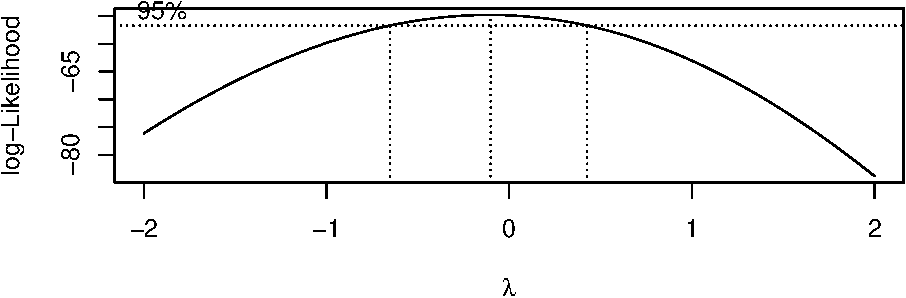
\includegraphics{Statistical_Methods_II_files/figure-latex/unnamed-chunk-159-1.pdf}

\section{Exercises}\label{exercises-7}

\begin{enumerate}
\def\labelenumi{\arabic{enumi}.}
\tightlist
\item
  Use the dataset \texttt{chickwts} in the \texttt{faraway} package.
  This was an experiment to determine which feed types result in the
  largest chickens. A set of 71 chicks were all randomly assigned one of
  six feed types and their weight in grams after six weeks was recorded.
  Determine whether there are differences in the weights of chickens
  according to their feed. Perform all necessary model diagnostics and
  examine the contrasts between each pair of feed levels. Summarize
  these results.
\end{enumerate}

\chapter{Two-way ANOVA}\label{two-way-anova}

\begin{Shaded}
\begin{Highlighting}[]
\CommentTok{# Load my usual packages}
\KeywordTok{library}\NormalTok{(MASS)     }\CommentTok{# for the boxcox function}
\KeywordTok{library}\NormalTok{(faraway)}
\KeywordTok{library}\NormalTok{(ggplot2)}
\KeywordTok{library}\NormalTok{(dplyr)}
\KeywordTok{library}\NormalTok{(ggfortify)}
\KeywordTok{library}\NormalTok{(multcompView)}
\end{Highlighting}
\end{Shaded}

Given a response that is predicted by two different categorical
variables. Suppose we denote the levels of the first factor as
\(\alpha_{i}\) and has \(I\) levels. The second factor has levels
\(\beta_{j}\) and has \(J\) levels. As usual we let
\(\epsilon_{ijk}\stackrel{iid}{\sim}N\left(0,\sigma^{2}\right)\), and we
wish to fit the model

\[y_{ijk}=\mu+\alpha_{i}+\beta_{j}+\epsilon_{ijk}\]

which has the main effects of each covariate or possibly the model with
the interaction
\[y_{ijk}=\mu+\alpha_{i}+\beta_{j}+\left(\alpha\beta\right)_{ij}+\epsilon_{ijk}\]

To consider what an interaction term might mean consider the role of
temperature and humidity on the amount of fungal growth. You might
expect to see data similar to this (where the numbers represent some
sort of measure of fungal growth):

\begin{longtable}[]{@{}llllll@{}}
\toprule
\begin{minipage}[b]{0.20\columnwidth}\raggedright\strut
\strut
\end{minipage} & \begin{minipage}[b]{0.12\columnwidth}\raggedright\strut
\strut
\end{minipage} & \begin{minipage}[b]{0.07\columnwidth}\raggedright\strut
5\%\strut
\end{minipage} & \begin{minipage}[b]{0.07\columnwidth}\raggedright\strut
30\%\strut
\end{minipage} & \begin{minipage}[b]{0.07\columnwidth}\raggedright\strut
60\%\strut
\end{minipage} & \begin{minipage}[b]{0.07\columnwidth}\raggedright\strut
90\%\strut
\end{minipage}\tabularnewline
\midrule
\endhead
\begin{minipage}[t]{0.20\columnwidth}\raggedright\strut
\strut
\end{minipage} & \begin{minipage}[t]{0.12\columnwidth}\raggedright\strut
\textbf{2C}\strut
\end{minipage} & \begin{minipage}[t]{0.07\columnwidth}\raggedright\strut
2\strut
\end{minipage} & \begin{minipage}[t]{0.07\columnwidth}\raggedright\strut
4\strut
\end{minipage} & \begin{minipage}[t]{0.07\columnwidth}\raggedright\strut
8\strut
\end{minipage} & \begin{minipage}[t]{0.07\columnwidth}\raggedright\strut
16\strut
\end{minipage}\tabularnewline
\begin{minipage}[t]{0.20\columnwidth}\raggedright\strut
Temperature\strut
\end{minipage} & \begin{minipage}[t]{0.12\columnwidth}\raggedright\strut
\textbf{10C}\strut
\end{minipage} & \begin{minipage}[t]{0.07\columnwidth}\raggedright\strut
3\strut
\end{minipage} & \begin{minipage}[t]{0.07\columnwidth}\raggedright\strut
9\strut
\end{minipage} & \begin{minipage}[t]{0.07\columnwidth}\raggedright\strut
27\strut
\end{minipage} & \begin{minipage}[t]{0.07\columnwidth}\raggedright\strut
81\strut
\end{minipage}\tabularnewline
\begin{minipage}[t]{0.20\columnwidth}\raggedright\strut
\strut
\end{minipage} & \begin{minipage}[t]{0.12\columnwidth}\raggedright\strut
\textbf{30C}\strut
\end{minipage} & \begin{minipage}[t]{0.07\columnwidth}\raggedright\strut
4\strut
\end{minipage} & \begin{minipage}[t]{0.07\columnwidth}\raggedright\strut
16\strut
\end{minipage} & \begin{minipage}[t]{0.07\columnwidth}\raggedright\strut
64\strut
\end{minipage} & \begin{minipage}[t]{0.07\columnwidth}\raggedright\strut
256\strut
\end{minipage}\tabularnewline
\bottomrule
\end{longtable}

In this case we see that increased humidity increases the amount of
fungal growth, but the amount of increase depends on the temperature. At
2 C, the increase is humidity increases are significant, but at 10 C the
increases are larger, and at 30 C the increases are larger yet. The
effect of changing from one humidity level to the next \emph{depends on
which temperature level we are at}. This change in effect of humidity is
an interaction effect. A memorable example is that chocolate by itself
is good. Strawberries by themselves are also good. But the combination
of chocolate and strawberries is a delight greater than the sum of the
individual treats.

We can look at a graph of the Humidity and Temperature vs the Response
and see the effect of increasing humidity changes based on the
temperature level. Just as in the ANCOVA model, the interaction
manifested itself in non-parallel slopes, the interaction manifests
itself in non-parallel slopes when I connect the dots across the factor
levels.

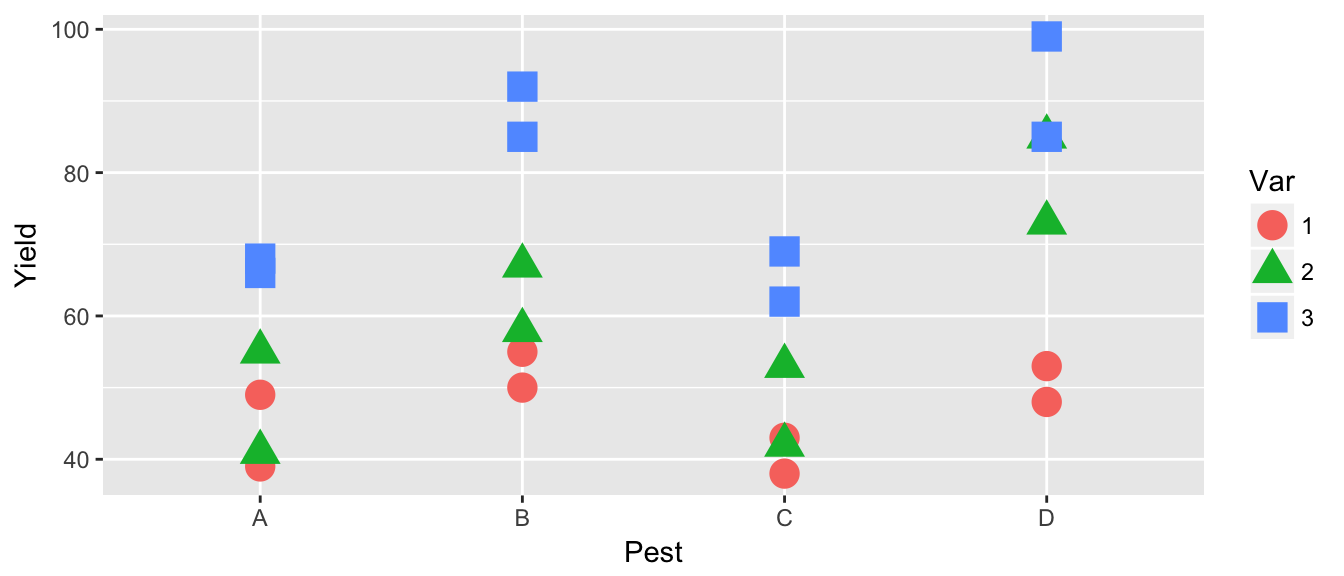
\includegraphics{Statistical_Methods_II_files/figure-latex/unnamed-chunk-162-1.pdf}

Unfortunately the presence of a significant interaction term in the
model makes interpretation difficult, but examining the interaction
plots can be quite helpful in understanding the effects. Notice in this
example, we 3 levels of temperature and 4 levels of humidity for a total
of 12 different possible treatment combinations. In general I will refer
to these combinations as cells.

\section{Orthogonality}\label{orthogonality}

When designing an experiment, I want to make sure than none of my
covariates are confounded with each other and I'd also like for them to
not be correlated. Consider the following three experimental designs,
where the number in each bin is the number of subjects of that type. I
am interested in testing 2 different drugs and studying its effect on
heart disease within the gender groups.

\begin{longtable}[]{@{}lllllll@{}}
\toprule
\begin{minipage}[t]{0.13\columnwidth}\raggedright\strut
Design 1\strut
\end{minipage} & \begin{minipage}[t]{0.08\columnwidth}\raggedright\strut
Males\strut
\end{minipage} & \begin{minipage}[t]{0.09\columnwidth}\raggedright\strut
Females\strut
\end{minipage} & \begin{minipage}[t]{0.22\columnwidth}\raggedright\strut
\strut
\end{minipage} & \begin{minipage}[t]{0.13\columnwidth}\raggedright\strut
Design 2\strut
\end{minipage} & \begin{minipage}[t]{0.07\columnwidth}\raggedright\strut
Males\strut
\end{minipage} & \begin{minipage}[t]{0.09\columnwidth}\raggedright\strut
Females\strut
\end{minipage}\tabularnewline
\begin{minipage}[t]{0.13\columnwidth}\raggedright\strut
Treatment A\strut
\end{minipage} & \begin{minipage}[t]{0.08\columnwidth}\raggedright\strut
0\strut
\end{minipage} & \begin{minipage}[t]{0.09\columnwidth}\raggedright\strut
10\strut
\end{minipage} & \begin{minipage}[t]{0.22\columnwidth}\raggedright\strut
\strut
\end{minipage} & \begin{minipage}[t]{0.13\columnwidth}\raggedright\strut
Treatment A\strut
\end{minipage} & \begin{minipage}[t]{0.07\columnwidth}\raggedright\strut
1\strut
\end{minipage} & \begin{minipage}[t]{0.09\columnwidth}\raggedright\strut
9\strut
\end{minipage}\tabularnewline
\begin{minipage}[t]{0.13\columnwidth}\raggedright\strut
Treatment B\strut
\end{minipage} & \begin{minipage}[t]{0.08\columnwidth}\raggedright\strut
6\strut
\end{minipage} & \begin{minipage}[t]{0.09\columnwidth}\raggedright\strut
0\strut
\end{minipage} & \begin{minipage}[t]{0.22\columnwidth}\raggedright\strut
\strut
\end{minipage} & \begin{minipage}[t]{0.13\columnwidth}\raggedright\strut
Treatment B\strut
\end{minipage} & \begin{minipage}[t]{0.07\columnwidth}\raggedright\strut
5\strut
\end{minipage} & \begin{minipage}[t]{0.09\columnwidth}\raggedright\strut
1\strut
\end{minipage}\tabularnewline
\bottomrule
\end{longtable}

\(\vspace{.2cm}\)

\begin{longtable}[]{@{}lllllll@{}}
\toprule
\begin{minipage}[t]{0.13\columnwidth}\raggedright\strut
Design 3\strut
\end{minipage} & \begin{minipage}[t]{0.08\columnwidth}\raggedright\strut
Males\strut
\end{minipage} & \begin{minipage}[t]{0.09\columnwidth}\raggedright\strut
Females\strut
\end{minipage} & \begin{minipage}[t]{0.22\columnwidth}\raggedright\strut
\strut
\end{minipage} & \begin{minipage}[t]{0.13\columnwidth}\raggedright\strut
Design 4\strut
\end{minipage} & \begin{minipage}[t]{0.07\columnwidth}\raggedright\strut
Males\strut
\end{minipage} & \begin{minipage}[t]{0.09\columnwidth}\raggedright\strut
Females\strut
\end{minipage}\tabularnewline
\begin{minipage}[t]{0.13\columnwidth}\raggedright\strut
Treatment A\strut
\end{minipage} & \begin{minipage}[t]{0.08\columnwidth}\raggedright\strut
3\strut
\end{minipage} & \begin{minipage}[t]{0.09\columnwidth}\raggedright\strut
5\strut
\end{minipage} & \begin{minipage}[t]{0.22\columnwidth}\raggedright\strut
\strut
\end{minipage} & \begin{minipage}[t]{0.13\columnwidth}\raggedright\strut
Treatment A\strut
\end{minipage} & \begin{minipage}[t]{0.07\columnwidth}\raggedright\strut
4\strut
\end{minipage} & \begin{minipage}[t]{0.09\columnwidth}\raggedright\strut
4\strut
\end{minipage}\tabularnewline
\begin{minipage}[t]{0.13\columnwidth}\raggedright\strut
Treatment B\strut
\end{minipage} & \begin{minipage}[t]{0.08\columnwidth}\raggedright\strut
3\strut
\end{minipage} & \begin{minipage}[t]{0.09\columnwidth}\raggedright\strut
5\strut
\end{minipage} & \begin{minipage}[t]{0.22\columnwidth}\raggedright\strut
\strut
\end{minipage} & \begin{minipage}[t]{0.13\columnwidth}\raggedright\strut
Treatment B\strut
\end{minipage} & \begin{minipage}[t]{0.07\columnwidth}\raggedright\strut
4\strut
\end{minipage} & \begin{minipage}[t]{0.09\columnwidth}\raggedright\strut
4\strut
\end{minipage}\tabularnewline
\bottomrule
\end{longtable}

\begin{enumerate}
\def\labelenumi{\arabic{enumi}.}
\item
  This design is very bad. Because we have no males taking drug 1, and
  no females taking drug 2, we can't say if any observed differences are
  due to the effect of drug 1 versus 2, or gender. When this situation
  happens, we say that the gender effect is confounded with the drug
  effect.
\item
  This design is not much better. Because we only have one observation
  in the Male-Drug 1 group, any inference we make about the effect of
  drug 1 on males is based on one observation. In general that is a bad
  idea.
\item
  Design 3 is better than the previous 2 because it evenly distributes
  the males and females among the two drug categories. However, it seems
  wasteful to have more females than males because estimating average of
  the male groups, I only have 6 observations while I have 10 females.
\item
  This is the ideal design, with equal numbers of observations in each
  gender-drug group.
\end{enumerate}

Designs 3 and 4 are good because the correlation among my predictors is
0. In design 1, the drug covariate is perfectly correlated to the gender
covariate. The correlation is less in design 2, but is zero in designs 3
and 4.We could show this by calculating the design matrix for each
design and calculating the correlation coefficients between each of
pairs of columns.

Having an orthogonal design with equal numbers of observations in each
group has many nice ramifications. Most importantly, with an orthogonal
design, the interpretation of parameter is not dependent on what other
factors are in the model. Balanced designs are also usually optimal in
the sense that the variances of \(\hat{\boldsymbol{\beta}}\) are as
small as possible given the number of observations we have (barring any
other \emph{a priori} information).

\section{Main Effects Model}\label{main-effects-model}

In the one factor ANOVA case, the additional degrees of freedom used by
adding a factor with \(I\) levels was \(I-1\). In the case that we
consider two factors with the first factor having \(I\) levels and the
second factor having \(J\) levels, then model
\[y_{ijk}=\mu+\alpha_{i}+\beta_{j}+\epsilon_{ijk}\] adds \((I-1)+(J-1)\)
parameters to the model because both \(\alpha_{1}=\beta_{1}=0\).

\begin{itemize}
\item
  The intercept term, \(\mu\) is the reference point for all the other
  parameters. This is the expected value for an observation in the first
  level of factor 1 and the first level of factor two.
\item
  \(\alpha_{i}\) is the amount you expect the response to increase when
  changing from factor 1 level 1, to factor 1 level i (while the second
  factor is held constant).
\item
  \(\beta_{j}\) is the amount you expect the response to increase when
  changing from factor 2 level 1 to factor 2 level j (while the first
  factor is held constant).
\end{itemize}

Referring back to the fungus example, let the \(\alpha_{i}\) values be
associated with changes in humidity and \(\beta_{j}\) values be
associated with changes in temperature levels. Then the expected value
of each treatment combination is

\begin{longtable}[]{@{}lllll@{}}
\toprule
\begin{minipage}[b]{0.08\columnwidth}\raggedright\strut
\strut
\end{minipage} & \begin{minipage}[b]{0.14\columnwidth}\raggedright\strut
\textbf{5\%}\strut
\end{minipage} & \begin{minipage}[b]{0.22\columnwidth}\raggedright\strut
\textbf{30\%}\strut
\end{minipage} & \begin{minipage}[b]{0.21\columnwidth}\raggedright\strut
\textbf{60\%}\strut
\end{minipage} & \begin{minipage}[b]{0.21\columnwidth}\raggedright\strut
\textbf{90\%}\strut
\end{minipage}\tabularnewline
\midrule
\endhead
\begin{minipage}[t]{0.08\columnwidth}\raggedright\strut
\textbf{2C}\strut
\end{minipage} & \begin{minipage}[t]{0.14\columnwidth}\raggedright\strut
\(\mu+0+0\)\strut
\end{minipage} & \begin{minipage}[t]{0.22\columnwidth}\raggedright\strut
\(\mu+\alpha_2+0\)\strut
\end{minipage} & \begin{minipage}[t]{0.21\columnwidth}\raggedright\strut
\(\mu+\alpha_3+0\)\strut
\end{minipage} & \begin{minipage}[t]{0.21\columnwidth}\raggedright\strut
\(\mu+\alpha_4+0\)\strut
\end{minipage}\tabularnewline
\begin{minipage}[t]{0.08\columnwidth}\raggedright\strut
\textbf{10C}\strut
\end{minipage} & \begin{minipage}[t]{0.14\columnwidth}\raggedright\strut
\(\mu+0+\beta_2\)\strut
\end{minipage} & \begin{minipage}[t]{0.22\columnwidth}\raggedright\strut
\(\mu+\alpha_2+\beta_2\)\strut
\end{minipage} & \begin{minipage}[t]{0.21\columnwidth}\raggedright\strut
\(\mu+\alpha_3+\beta_2\)\strut
\end{minipage} & \begin{minipage}[t]{0.21\columnwidth}\raggedright\strut
\(\mu+\alpha_4+\beta_2\)\strut
\end{minipage}\tabularnewline
\begin{minipage}[t]{0.08\columnwidth}\raggedright\strut
\textbf{30C}\strut
\end{minipage} & \begin{minipage}[t]{0.14\columnwidth}\raggedright\strut
\(\mu+0+\beta_3\)\strut
\end{minipage} & \begin{minipage}[t]{0.22\columnwidth}\raggedright\strut
\(\mu+\alpha_2+\beta_3\)\strut
\end{minipage} & \begin{minipage}[t]{0.21\columnwidth}\raggedright\strut
\(\mu+\alpha_3+\beta_3\)\strut
\end{minipage} & \begin{minipage}[t]{0.21\columnwidth}\raggedright\strut
\(\mu+\alpha_4+\beta_3\)\strut
\end{minipage}\tabularnewline
\bottomrule
\end{longtable}

\subsection{Example - Fruit Trees}\label{example---fruit-trees}

An experiment was conducted to determine the effects of four different
pesticides on the yield of fruit from three different varieties of a
citrus tree. Eight trees of each variety were randomly selected from an
orchard. The four pesticides were randomly assigned to two trees of each
variety and applications were made according to recommended levels.
Yields of fruit (in bushels) were obtained after the test period.

Critically notice that we have equal number of observations for each
treatment combination.

\begin{Shaded}
\begin{Highlighting}[]
\CommentTok{# Typing the data in by hand because I got this example from a really old text book...}
\NormalTok{Pesticide <-}\StringTok{ }\KeywordTok{factor}\NormalTok{(}\KeywordTok{c}\NormalTok{(}\StringTok{'A'}\NormalTok{,}\StringTok{'B'}\NormalTok{,}\StringTok{'C'}\NormalTok{,}\StringTok{'D'}\NormalTok{)) }
\NormalTok{Variety <-}\StringTok{ }\KeywordTok{factor}\NormalTok{(}\KeywordTok{c}\NormalTok{(}\StringTok{'1'}\NormalTok{,}\StringTok{'2'}\NormalTok{,}\StringTok{'3'}\NormalTok{)) }
\NormalTok{fruit <-}\StringTok{ }\KeywordTok{data.frame}\NormalTok{( }\KeywordTok{expand.grid}\NormalTok{(}\DataTypeTok{rep=}\DecValTok{1}\NormalTok{:}\DecValTok{2}\NormalTok{, }\DataTypeTok{Pest=}\NormalTok{Pesticide, }\DataTypeTok{Var=}\NormalTok{Variety) ) }
\NormalTok{fruit$Yield <-}\StringTok{ }\KeywordTok{c}\NormalTok{(}\DecValTok{49}\NormalTok{,}\DecValTok{39}\NormalTok{,}\DecValTok{50}\NormalTok{,}\DecValTok{55}\NormalTok{,}\DecValTok{43}\NormalTok{,}\DecValTok{38}\NormalTok{,}\DecValTok{53}\NormalTok{,}\DecValTok{48}\NormalTok{,}\DecValTok{55}\NormalTok{,}\DecValTok{41}\NormalTok{,}\DecValTok{67}\NormalTok{,}\DecValTok{58}\NormalTok{,}\DecValTok{53}\NormalTok{,}\DecValTok{42}\NormalTok{,}\DecValTok{85}\NormalTok{,}\DecValTok{73}\NormalTok{,}\DecValTok{66}\NormalTok{,}\DecValTok{68}\NormalTok{,}\DecValTok{85}\NormalTok{,}\DecValTok{92}\NormalTok{,}\DecValTok{69}\NormalTok{,}\DecValTok{62}\NormalTok{,}\DecValTok{85}\NormalTok{,}\DecValTok{99}\NormalTok{)}
\end{Highlighting}
\end{Shaded}

The first thing to do (as always) is to look at our data

\begin{Shaded}
\begin{Highlighting}[]
\KeywordTok{ggplot}\NormalTok{(fruit, }\KeywordTok{aes}\NormalTok{(}\DataTypeTok{x=}\NormalTok{Pest, }\DataTypeTok{color=}\NormalTok{Var, }\DataTypeTok{y=}\NormalTok{Yield, }\DataTypeTok{shape=}\NormalTok{Var)) +}\StringTok{ }
\StringTok{    }\KeywordTok{geom_point}\NormalTok{(}\DataTypeTok{size=}\DecValTok{5}\NormalTok{) }
\end{Highlighting}
\end{Shaded}

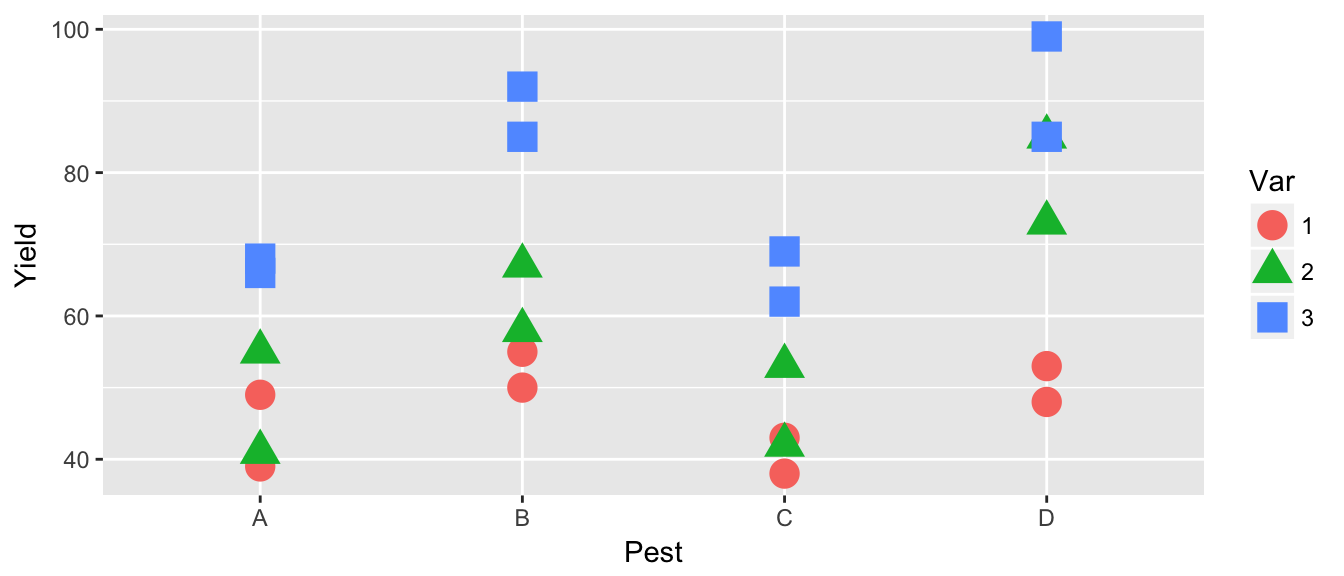
\includegraphics{Statistical_Methods_II_files/figure-latex/unnamed-chunk-164-1.pdf}

The first thing we notice is that pesticides B and D seem to be better
than the others and that variety 3 seems to be the best producer. The
effect of pesticide treatment seems consistent between varieties, so we
don't expect that the interaction effect will be significant. We next
fit a linear model and look at the diagnostic plots.

\begin{Shaded}
\begin{Highlighting}[]
\NormalTok{m3 <-}\StringTok{ }\KeywordTok{lm}\NormalTok{(Yield ~}\StringTok{ }\NormalTok{Var +}\StringTok{ }\NormalTok{Pest, }\DataTypeTok{data=}\NormalTok{fruit)}
\KeywordTok{autoplot}\NormalTok{(m3, }\DataTypeTok{which=}\DecValTok{1}\NormalTok{:}\DecValTok{2}\NormalTok{)}
\end{Highlighting}
\end{Shaded}

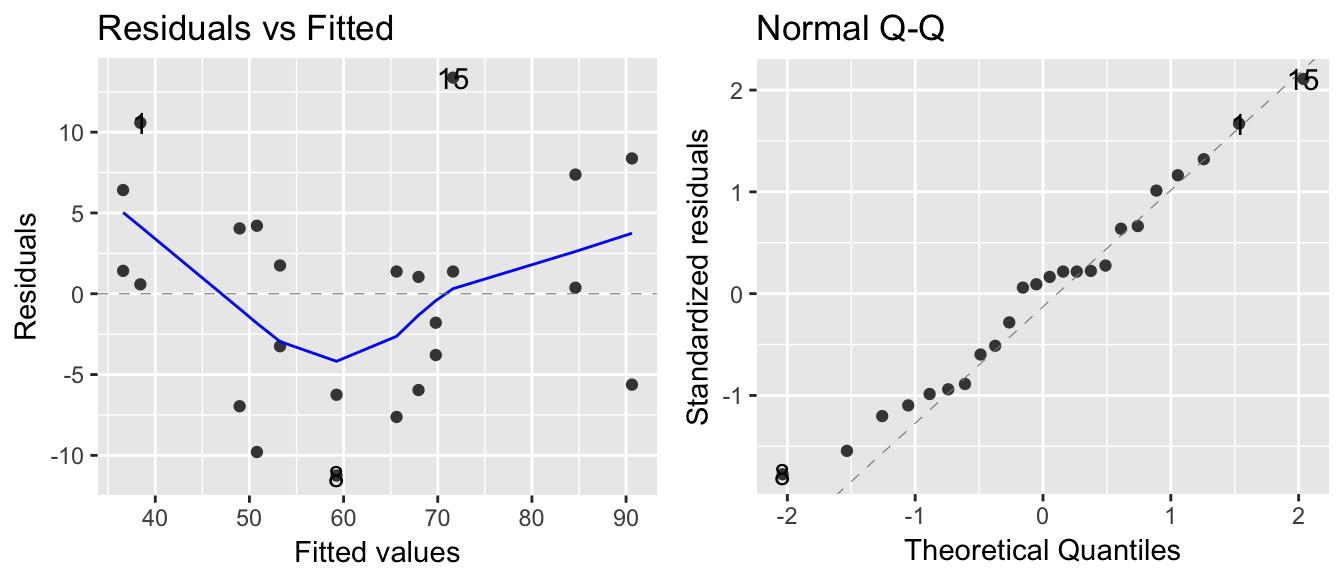
\includegraphics{Statistical_Methods_II_files/figure-latex/unnamed-chunk-165-1.pdf}

There might be a little curvature in the fitted vs residuals, but
because we can't fit a polynomial to a categorical variable, and the
QQ-plot looks good, we'll ignore it for now and eventually consider an
interaction term. Just for fun, we can examine the smaller models with
just Variety or Pesticide.

\begin{Shaded}
\begin{Highlighting}[]
\NormalTok{m1 <-}\StringTok{ }\KeywordTok{lm}\NormalTok{(Yield ~}\StringTok{ }\NormalTok{Var, }\DataTypeTok{data=}\NormalTok{fruit)}
\NormalTok{m2 <-}\StringTok{ }\KeywordTok{lm}\NormalTok{(Yield ~}\StringTok{ }\NormalTok{Pest, }\DataTypeTok{data=}\NormalTok{fruit)}
\NormalTok{m3 <-}\StringTok{ }\KeywordTok{lm}\NormalTok{(Yield ~}\StringTok{ }\NormalTok{Var +}\StringTok{ }\NormalTok{Pest, }\DataTypeTok{data=}\NormalTok{fruit)}
\KeywordTok{summary}\NormalTok{(m1)$coef  %>%}\StringTok{ }\KeywordTok{round}\NormalTok{(}\DataTypeTok{digits=}\DecValTok{3}\NormalTok{)}
\end{Highlighting}
\end{Shaded}

\begin{verbatim}
##             Estimate Std. Error t value Pr(>|t|)
## (Intercept)   46.875      4.359  10.754    0.000
## Var2          12.375      6.164   2.008    0.058
## Var3          31.375      6.164   5.090    0.000
\end{verbatim}

\begin{Shaded}
\begin{Highlighting}[]
\KeywordTok{summary}\NormalTok{(m2)$coef  %>%}\StringTok{ }\KeywordTok{round}\NormalTok{(}\DataTypeTok{digits=}\DecValTok{3}\NormalTok{)}
\end{Highlighting}
\end{Shaded}

\begin{verbatim}
##             Estimate Std. Error t value Pr(>|t|)
## (Intercept)   53.000      6.429   8.243    0.000
## PestB         14.833      9.093   1.631    0.118
## PestC         -1.833      9.093  -0.202    0.842
## PestD         20.833      9.093   2.291    0.033
\end{verbatim}

\begin{Shaded}
\begin{Highlighting}[]
\KeywordTok{summary}\NormalTok{(m3)$coef  %>%}\StringTok{ }\KeywordTok{round}\NormalTok{(}\DataTypeTok{digits=}\DecValTok{3}\NormalTok{)}
\end{Highlighting}
\end{Shaded}

\begin{verbatim}
##             Estimate Std. Error t value Pr(>|t|)
## (Intercept)   38.417      3.660  10.497    0.000
## Var2          12.375      3.660   3.381    0.003
## Var3          31.375      3.660   8.573    0.000
## PestB         14.833      4.226   3.510    0.003
## PestC         -1.833      4.226  -0.434    0.670
## PestD         20.833      4.226   4.930    0.000
\end{verbatim}

Notice that the affects for Variety and Pesticide are the same
\emph{whether or not the other is in the model}. This is due to the
orthogonal design of the experiment and makes it much easier to
interpret the main effects of Variety and Pesticide.

\subsection{ANOVA Table}\label{anova-table}

Most statistical software will produce an analysis of variance table
when fitting a two-way ANOVA. This table is very similar to the analysis
of variance table we have seen in the one-way ANOVA, but has several
rows which correspond to the additional factors added to the model.

Consider the two-way ANOVA with factors \(A\) and \(B\) which have
levels \(I\) and \(J\) discrete levels respectively. For convenience let
\(RSS_{1}\) is the residual sum of squares of the intercept-only model,
and \(RSS_{A}\) be the residual sum of squares for the model with just
the main effect of factor \(A\), and \(RSS_{A+B}\) be the residual sum
of squares of the model with both main effects. Finally assume that we
have a total of \(n\) observations. The ANOVA table for this model is as
follows:

\begin{longtable}[]{@{}llllll@{}}
\toprule
\begin{minipage}[b]{0.07\columnwidth}\raggedright\strut
Source\strut
\end{minipage} & \begin{minipage}[b]{0.10\columnwidth}\raggedright\strut
df\strut
\end{minipage} & \begin{minipage}[b]{0.17\columnwidth}\raggedright\strut
Sum of Sq (SS)\strut
\end{minipage} & \begin{minipage}[b]{0.16\columnwidth}\raggedright\strut
Mean Sq\strut
\end{minipage} & \begin{minipage}[b]{0.09\columnwidth}\raggedright\strut
F\strut
\end{minipage} & \begin{minipage}[b]{0.24\columnwidth}\raggedright\strut
p-value\strut
\end{minipage}\tabularnewline
\midrule
\endhead
\begin{minipage}[t]{0.07\columnwidth}\raggedright\strut
\textbf{A}\strut
\end{minipage} & \begin{minipage}[t]{0.10\columnwidth}\raggedright\strut
\(df_A=I-1\)\strut
\end{minipage} & \begin{minipage}[t]{0.17\columnwidth}\raggedright\strut
\(SS_A = RSS_1 - RSS_A\)\strut
\end{minipage} & \begin{minipage}[t]{0.16\columnwidth}\raggedright\strut
\(MS_A = SS_A / df_A\)\strut
\end{minipage} & \begin{minipage}[t]{0.09\columnwidth}\raggedright\strut
\(MS_A / MSE\)\strut
\end{minipage} & \begin{minipage}[t]{0.24\columnwidth}\raggedright\strut
\(P\left( F_{df_A, df_e} > F_A \right)\)\strut
\end{minipage}\tabularnewline
\begin{minipage}[t]{0.07\columnwidth}\raggedright\strut
\textbf{B}\strut
\end{minipage} & \begin{minipage}[t]{0.10\columnwidth}\raggedright\strut
\(df_B=J-1\)\strut
\end{minipage} & \begin{minipage}[t]{0.17\columnwidth}\raggedright\strut
\(SS_B = RSS_A - RSS_{A+B}\)\strut
\end{minipage} & \begin{minipage}[t]{0.16\columnwidth}\raggedright\strut
\(MS_B = SS_B / df_B\)\strut
\end{minipage} & \begin{minipage}[t]{0.09\columnwidth}\raggedright\strut
\(MS_B / MSE\)\strut
\end{minipage} & \begin{minipage}[t]{0.24\columnwidth}\raggedright\strut
\(P\left( F_{df_B, df_e} > F_B \right)\)\strut
\end{minipage}\tabularnewline
\begin{minipage}[t]{0.07\columnwidth}\raggedright\strut
\textbf{Error}\strut
\end{minipage} & \begin{minipage}[t]{0.10\columnwidth}\raggedright\strut
\(df_e=n-I-J+1\)\strut
\end{minipage} & \begin{minipage}[t]{0.17\columnwidth}\raggedright\strut
\(RSS_{A+B}\)\strut
\end{minipage} & \begin{minipage}[t]{0.16\columnwidth}\raggedright\strut
\(MSE = RSS_{A+B} / df_e\)\strut
\end{minipage} & \begin{minipage}[t]{0.09\columnwidth}\raggedright\strut
\strut
\end{minipage} & \begin{minipage}[t]{0.24\columnwidth}\raggedright\strut
\strut
\end{minipage}\tabularnewline
\bottomrule
\end{longtable}

\emph{Note, if the table is cut off, you can change decrease your font
size and have it all show up\ldots{}}

This arrangement of the ANOVA table is referred to as ``Type I'' sum of
squares.

We can examine this table in the fruit trees example using the anova()
command but just passing a single model.

\begin{Shaded}
\begin{Highlighting}[]
\NormalTok{m4 <-}\StringTok{ }\KeywordTok{lm}\NormalTok{(Yield ~}\StringTok{ }\NormalTok{Var +}\StringTok{ }\NormalTok{Pest, }\DataTypeTok{data=}\NormalTok{fruit)}
\KeywordTok{anova}\NormalTok{( m4 )}
\end{Highlighting}
\end{Shaded}

\begin{verbatim}
## Analysis of Variance Table
## 
## Response: Yield
##           Df Sum Sq Mean Sq F value    Pr(>F)    
## Var        2 3996.1 1998.04  37.292 3.969e-07 ***
## Pest       3 2227.5  742.49  13.858 6.310e-05 ***
## Residuals 18  964.4   53.58                      
## ---
## Signif. codes:  0 '***' 0.001 '**' 0.01 '*' 0.05 '.' 0.1 ' ' 1
\end{verbatim}

We might think that this is the same as fitting three nested models and
running an F-test on each successive pairs of models, but it isn't.
While both will give the same Sums of Squares, the F statistics are
different because the MSE of the complex model is different. In
particular, the F-statistics are larger and thus the p-values are
smaller for detecting significant effects.

\begin{Shaded}
\begin{Highlighting}[]
\NormalTok{m1 <-}\StringTok{ }\KeywordTok{lm}\NormalTok{(Yield ~}\StringTok{ }\DecValTok{1}\NormalTok{, }\DataTypeTok{data=}\NormalTok{fruit)}
\NormalTok{m2 <-}\StringTok{ }\KeywordTok{lm}\NormalTok{(Yield ~}\StringTok{ }\NormalTok{Var, }\DataTypeTok{data=}\NormalTok{fruit)}
\NormalTok{m3 <-}\StringTok{ }\KeywordTok{lm}\NormalTok{(Yield ~}\StringTok{ }\NormalTok{Var +}\StringTok{ }\NormalTok{Pest, }\DataTypeTok{data=}\NormalTok{fruit)}
\KeywordTok{anova}\NormalTok{( m1, m2 )}
\end{Highlighting}
\end{Shaded}

\begin{verbatim}
## Analysis of Variance Table
## 
## Model 1: Yield ~ 1
## Model 2: Yield ~ Var
##   Res.Df    RSS Df Sum of Sq      F    Pr(>F)    
## 1     23 7188.0                                  
## 2     21 3191.9  2    3996.1 13.146 0.0001987 ***
## ---
## Signif. codes:  0 '***' 0.001 '**' 0.01 '*' 0.05 '.' 0.1 ' ' 1
\end{verbatim}

\begin{Shaded}
\begin{Highlighting}[]
\KeywordTok{anova}\NormalTok{( m2, m3 )}
\end{Highlighting}
\end{Shaded}

\begin{verbatim}
## Analysis of Variance Table
## 
## Model 1: Yield ~ Var
## Model 2: Yield ~ Var + Pest
##   Res.Df    RSS Df Sum of Sq      F   Pr(>F)    
## 1     21 3191.9                                 
## 2     18  964.4  3    2227.5 13.858 6.31e-05 ***
## ---
## Signif. codes:  0 '***' 0.001 '**' 0.01 '*' 0.05 '.' 0.1 ' ' 1
\end{verbatim}

\subsection{Estimating Contrasts}\label{estimating-contrasts}

As in the one-way ANOVA, we are interested in which factor levels
differ. For example, we might suspect that it makes sense to group
pesticides B and D together and claim that they are better than the
group of A and C.

Just as we did in the one-way ANOVA model, this is such a common thing
to do that there is an easy way to do this, using \texttt{TukeyHSD},
which requires us coerce our model output to an \texttt{aov} object. We
could specify all of the contrasts by hand and use \texttt{glht()} in
the \texttt{multcomp} package to calculate all of the contrasts, but
using \texttt{TukeyHSD} will be simpler.

\begin{Shaded}
\begin{Highlighting}[]
\NormalTok{m3 <-}\StringTok{ }\KeywordTok{lm}\NormalTok{(Yield ~}\StringTok{ }\NormalTok{Var +}\StringTok{ }\NormalTok{Pest, }\DataTypeTok{data=}\NormalTok{fruit)}
\KeywordTok{TukeyHSD}\NormalTok{(}\KeywordTok{aov}\NormalTok{(m3))}
\end{Highlighting}
\end{Shaded}

\begin{verbatim}
##   Tukey multiple comparisons of means
##     95% family-wise confidence level
## 
## Fit: aov(formula = m3)
## 
## $Var
##       diff       lwr      upr     p adj
## 2-1 12.375  3.034405 21.71559 0.0088734
## 3-1 31.375 22.034405 40.71559 0.0000003
## 3-2 19.000  9.659405 28.34059 0.0001735
## 
## $Pest
##           diff        lwr       upr     p adj
## B-A  14.833333   2.889267 26.777399 0.0121713
## C-A  -1.833333 -13.777399 10.110733 0.9718552
## D-A  20.833333   8.889267 32.777399 0.0005728
## C-B -16.666667 -28.610733 -4.722601 0.0047986
## D-B   6.000000  -5.944066 17.944066 0.5037838
## D-C  22.666667  10.722601 34.610733 0.0002286
\end{verbatim}

The output from the TukeyHSD is quite useful, but it would be nice to
generate the data frame indicating group differences similar to what we
did in the one-way ANOVA. We will use the exact same function we had
before:

\begin{Shaded}
\begin{Highlighting}[]
\CommentTok{#' Create a data frame with significant groupings }
\CommentTok{#'}
\CommentTok{#' This function runs TukeyHSD on the input model and then creates a data frame}
\CommentTok{#' with a column for the factor and a second for the Significance Group}
\CommentTok{#' }
\CommentTok{#' @param model The output of a lm() or aov() call that can be coerced to an aov object.}
\CommentTok{#' @param variable The variable of interest.}
\CommentTok{#' @output A data frame with a column for factor and another for the signicance group.}
\NormalTok{make_TukeyHSD_letters <-}\StringTok{ }\NormalTok{function(model, variable)\{ }
  \NormalTok{Tukey <-}\StringTok{ }\KeywordTok{TukeyHSD}\NormalTok{(}\KeywordTok{aov}\NormalTok{(model))[[variable]]}
  \NormalTok{temp <-}\StringTok{ }\NormalTok{Tukey[,}\StringTok{'p adj'}\NormalTok{] %>%}
\StringTok{    }\KeywordTok{vec2mat}\NormalTok{() %>%}
\StringTok{    }\KeywordTok{multcompLetters}\NormalTok{()}
  \NormalTok{out <-}\StringTok{ }\KeywordTok{data.frame}\NormalTok{(}\DataTypeTok{group =} \KeywordTok{names}\NormalTok{(temp$Letters), }\DataTypeTok{SigGroup=}\NormalTok{temp$Letters)}
  \KeywordTok{colnames}\NormalTok{(out)[}\DecValTok{1}\NormalTok{] <-}\StringTok{ }\NormalTok{variable}
  \NormalTok{out}
\NormalTok{\}  }
\end{Highlighting}
\end{Shaded}

\begin{Shaded}
\begin{Highlighting}[]
\KeywordTok{make_TukeyHSD_letters}\NormalTok{( m3, }\StringTok{'Var'}\NormalTok{)}
\end{Highlighting}
\end{Shaded}

\begin{verbatim}
##   Var SigGroup
## 2   2        a
## 3   3        b
## 1   1        c
\end{verbatim}

\begin{Shaded}
\begin{Highlighting}[]
\KeywordTok{make_TukeyHSD_letters}\NormalTok{( m3, }\StringTok{'Pest'}\NormalTok{)}
\end{Highlighting}
\end{Shaded}

\begin{verbatim}
##   Pest SigGroup
## B    B        a
## C    C        b
## D    D        a
## A    A        b
\end{verbatim}

So we see that each variety is significantly different from all the
others and among the pesticides, \(A\) and \(C\) are indistigishable as
are \(B\) and \(D\), but there is a difference between the \(A,C\) and
\(B,D\) groups.

\section{Interaction Model}\label{interaction-model}

When the model contains the interaction of the two factors, our model is
written as
\[y_{ijk}=\mu+\alpha_{i}+\beta_{j}+\left(\alpha\beta\right)_{ij}+\epsilon_{ijk}\]

Interpreting effects effects can be very tricky. Under the interaction,
the effect of changing from factor 1 level 1 to factor 1 level \(i\)
depends on what level of factor 2 is. In essence, we are fitting a model
that allows each of the \(I\times J\) cells in my model to vary
independently. As such, the model has a total of \(I\times J\)
parameters but because the model without interactions had
\(1+(I-1)+(J-1)\) terms in it, the interaction is adding \(df_{AB}\)
parameters. We can solve for this via: \[\begin{aligned}
I\times J   &=  1+(I-1)+(J-1)+df_{AB} \\
I\times J   &=  I+J-1+df_{AB} \\
IJ-I-J    &=    -1+df_{AB} \\
I(J-1)-J    &=  -1+df_{AB} \\
I(J-1)-J+1  &=  df_{AB}  \\
I(J-1)-(J-1)    &=  df_{AB} \\
(I-1)(J-1)  &=  df_{AB} 
\end{aligned}\]

This makes sense because the first factor added \((I-1)\) columns to the
design matrix and an interaction with a continuous covariate just
multiplied the columns of the factor by the single column of the
continuous covariate. Creating an interaction of two factors multiplies
each column of the first factor by all the columns defined by the second
factor.

The expected value of the \(ij\) combination is
\(\mu+\alpha_{i}+\beta_{j}+\left(\alpha\beta\right)_{ij}\). Returning to
our fungus example, the expected means for each treatment under the
model with main effects and the interaction is

\begin{longtable}[]{@{}lllll@{}}
\toprule
\begin{minipage}[b]{0.04\columnwidth}\raggedright\strut
\strut
\end{minipage} & \begin{minipage}[b]{0.09\columnwidth}\raggedright\strut
\textbf{5\%}\strut
\end{minipage} & \begin{minipage}[b]{0.25\columnwidth}\raggedright\strut
\textbf{30\%}\strut
\end{minipage} & \begin{minipage}[b]{0.24\columnwidth}\raggedright\strut
\textbf{60\%}\strut
\end{minipage} & \begin{minipage}[b]{0.24\columnwidth}\raggedright\strut
\textbf{90\%}\strut
\end{minipage}\tabularnewline
\midrule
\endhead
\begin{minipage}[t]{0.04\columnwidth}\raggedright\strut
\textbf{2C}\strut
\end{minipage} & \begin{minipage}[t]{0.09\columnwidth}\raggedright\strut
\(\mu+0+0+0\)\strut
\end{minipage} & \begin{minipage}[t]{0.25\columnwidth}\raggedright\strut
\(\mu+\alpha_2+0+0\)\strut
\end{minipage} & \begin{minipage}[t]{0.24\columnwidth}\raggedright\strut
\(\mu+\alpha_3+0+0\)\strut
\end{minipage} & \begin{minipage}[t]{0.24\columnwidth}\raggedright\strut
\(\mu+\alpha_4+0+0\)\strut
\end{minipage}\tabularnewline
\begin{minipage}[t]{0.04\columnwidth}\raggedright\strut
\textbf{10C}\strut
\end{minipage} & \begin{minipage}[t]{0.09\columnwidth}\raggedright\strut
\(\mu+0+\beta_2+0\)\strut
\end{minipage} & \begin{minipage}[t]{0.25\columnwidth}\raggedright\strut
\(\mu+\alpha_2+\beta_2+\left(\alpha\beta\right)_{22}\)\strut
\end{minipage} & \begin{minipage}[t]{0.24\columnwidth}\raggedright\strut
\(\mu+\alpha_3+\beta_2+\left(\alpha\beta\right)_{32}\)\strut
\end{minipage} & \begin{minipage}[t]{0.24\columnwidth}\raggedright\strut
\(\mu+\alpha_4+\beta_2+\left(\alpha\beta\right)_{42}\)\strut
\end{minipage}\tabularnewline
\begin{minipage}[t]{0.04\columnwidth}\raggedright\strut
\textbf{30C}\strut
\end{minipage} & \begin{minipage}[t]{0.09\columnwidth}\raggedright\strut
\(\mu+0+\beta_3+0\)\strut
\end{minipage} & \begin{minipage}[t]{0.25\columnwidth}\raggedright\strut
\(\mu+\alpha_2+\beta_3+\left(\alpha\beta\right)_{23}\)\strut
\end{minipage} & \begin{minipage}[t]{0.24\columnwidth}\raggedright\strut
\(\mu+\alpha_3+\beta_2+\left(\alpha\beta\right)_{33}\)\strut
\end{minipage} & \begin{minipage}[t]{0.24\columnwidth}\raggedright\strut
\(\mu+\alpha_4+\beta_2+\left(\alpha\beta\right)_{43}\)\strut
\end{minipage}\tabularnewline
\bottomrule
\end{longtable}

Notice that we have added
\(6=3\cdot2=\left(4-1\right)\left(3-1\right)=\left(I-1\right)\left(J-1\right)\)
interaction parameters \(\left(\alpha\beta\right)_{ij}\) to the main
effects only model. The interaction model has \(p=12\) parameters, one
for each cell in my treatment array.

In general it is hard to interpret the meaning of \(\alpha_{i}\),
\(\beta_{j}\), and \(\left(\alpha\beta\right)_{ij}\) and the best way to
make sense of them is to look at the interaction plots.

\subsection{ANOVA Table}\label{anova-table-1}

Most statistical software will produce an analysis of variance table
when fitting a two-way ANOVA. This table is very similar to the analysis
of variance table we have seen in the one-way ANOVA, but has several
rows which correspond to the additional factors added to the model.

Consider the two-way ANOVA with factors \(A\) and \(B\) which have
levels \(I\) and \(J\) discrete levels respectively. For convenience let
\(RSS_{1}\) be the residual sum of squares of the intercept-only model,
and \(RSS_{A}\) be the residual sum of squares for the model with just
the main effect of factor \(A\). Likewise \(RSS_{A+B}\) and
\(RSS_{A*B}\) shall be the residual sum of squares of the model with
just the main effects and the model with main effects and the
interaction. Finally assume that we have a total of \(n\) observations.
The ANOVA table for this model is as follows:

\begin{longtable}[]{@{}llllll@{}}
\toprule
\begin{minipage}[b]{0.06\columnwidth}\raggedright\strut
\strut
\end{minipage} & \begin{minipage}[b]{0.11\columnwidth}\raggedright\strut
df\strut
\end{minipage} & \begin{minipage}[b]{0.17\columnwidth}\raggedright\strut
Sum Sq (SS)\strut
\end{minipage} & \begin{minipage}[b]{0.18\columnwidth}\raggedright\strut
MS\strut
\end{minipage} & \begin{minipage}[b]{0.08\columnwidth}\raggedright\strut
F\strut
\end{minipage} & \begin{minipage}[b]{0.22\columnwidth}\raggedright\strut
\(Pr(\ge F)\)\strut
\end{minipage}\tabularnewline
\midrule
\endhead
\begin{minipage}[t]{0.06\columnwidth}\raggedright\strut
\textbf{A}\strut
\end{minipage} & \begin{minipage}[t]{0.11\columnwidth}\raggedright\strut
\(df_A=I-1\)\strut
\end{minipage} & \begin{minipage}[t]{0.17\columnwidth}\raggedright\strut
\(SS_A = RSS_1 - RSS_A\)\strut
\end{minipage} & \begin{minipage}[t]{0.18\columnwidth}\raggedright\strut
\(MS_A = SS_A/df_A\)\strut
\end{minipage} & \begin{minipage}[t]{0.08\columnwidth}\raggedright\strut
\(MS_A / MSE\)\strut
\end{minipage} & \begin{minipage}[t]{0.22\columnwidth}\raggedright\strut
\(Pr(F_{df_A,df_{\epsilon}} \ge F_A\)\strut
\end{minipage}\tabularnewline
\begin{minipage}[t]{0.06\columnwidth}\raggedright\strut
\textbf{B}\strut
\end{minipage} & \begin{minipage}[t]{0.11\columnwidth}\raggedright\strut
\(df_B=J-1\)\strut
\end{minipage} & \begin{minipage}[t]{0.17\columnwidth}\raggedright\strut
\(SS_B = RSS_A - RSS_{A+B}\)\strut
\end{minipage} & \begin{minipage}[t]{0.18\columnwidth}\raggedright\strut
\(MS_B = SS_B/df_B\)\strut
\end{minipage} & \begin{minipage}[t]{0.08\columnwidth}\raggedright\strut
\(MS_B / MSE\)\strut
\end{minipage} & \begin{minipage}[t]{0.22\columnwidth}\raggedright\strut
\(Pr(F_{df_B,df_{\epsilon}} \ge F_B\)\strut
\end{minipage}\tabularnewline
\begin{minipage}[t]{0.06\columnwidth}\raggedright\strut
\textbf{AB}\strut
\end{minipage} & \begin{minipage}[t]{0.11\columnwidth}\raggedright\strut
\(df_{AB}=(I-1)(J-1)\)\strut
\end{minipage} & \begin{minipage}[t]{0.17\columnwidth}\raggedright\strut
\(SS_{A*B} = RSS_{A*B}-RSS_{A+B}\)\strut
\end{minipage} & \begin{minipage}[t]{0.18\columnwidth}\raggedright\strut
\(MS_{AB} = SS_{AB} / df_{AB}\)\strut
\end{minipage} & \begin{minipage}[t]{0.08\columnwidth}\raggedright\strut
\(MS_{AB} MSE\)\strut
\end{minipage} & \begin{minipage}[t]{0.22\columnwidth}\raggedright\strut
\(Pr(F_{df_{AB},df_{\epsilon}} \ge F_{AB}\)\strut
\end{minipage}\tabularnewline
\begin{minipage}[t]{0.06\columnwidth}\raggedright\strut
\textbf{Error}\strut
\end{minipage} & \begin{minipage}[t]{0.11\columnwidth}\raggedright\strut
\(df_{\epsilon}=n-IJ\)\strut
\end{minipage} & \begin{minipage}[t]{0.17\columnwidth}\raggedright\strut
\(RSS_{A*B}\)\strut
\end{minipage} & \begin{minipage}[t]{0.18\columnwidth}\raggedright\strut
\(MSE = RSS_{A*B} / df_{\epsilon}\)\strut
\end{minipage} & \begin{minipage}[t]{0.08\columnwidth}\raggedright\strut
\strut
\end{minipage} & \begin{minipage}[t]{0.22\columnwidth}\raggedright\strut
\strut
\end{minipage}\tabularnewline
\bottomrule
\end{longtable}

This arrangement of the ANOVA table is referred to as ``Type I'' sum of
squares. Type III sums of squares are the difference between the full
interaction model and the model removing each parameter group, even when
it doesn't make sense. For example in the Type III table,
\(SS_{A}=RSS_{B+A:B}-RSS_{A*B}\). There is an intermediate form of the
sums of squares called Type II, that when removing a main effect also
removes the higher order interaction. In the case of balanced
(orthogonal) designs, there is no difference between the different
types, but for non-balanced designs, the numbers will change. To access
these other types of sums of squares, use the \texttt{Anova()} function
in the package \texttt{car}.

\subsection{Example - Fruit Trees
(continued)}\label{example---fruit-trees-continued}

We next consider whether or not to include the interaction term to the
fruit tree model. We fit the model with the interaction and then graph
the results.

\begin{Shaded}
\begin{Highlighting}[]
\NormalTok{m4 <-}\StringTok{ }\KeywordTok{lm}\NormalTok{(Yield ~}\StringTok{ }\NormalTok{Var *}\StringTok{ }\NormalTok{Pest, }\DataTypeTok{data=}\NormalTok{fruit)}
\NormalTok{fruit$y.hat <-}\StringTok{ }\KeywordTok{predict}\NormalTok{(m4)}
\KeywordTok{ggplot}\NormalTok{(fruit, }\KeywordTok{aes}\NormalTok{(}\DataTypeTok{x=}\NormalTok{Pest, }\DataTypeTok{color=}\NormalTok{Var, }\DataTypeTok{shape=}\NormalTok{Var, }\DataTypeTok{y=}\NormalTok{Yield)) +}\StringTok{ }
\StringTok{    }\KeywordTok{geom_point}\NormalTok{(}\DataTypeTok{size=}\DecValTok{5}\NormalTok{) +}
\StringTok{    }\KeywordTok{geom_line}\NormalTok{(}\KeywordTok{aes}\NormalTok{(}\DataTypeTok{y=}\NormalTok{y.hat, }\DataTypeTok{x=}\KeywordTok{as.integer}\NormalTok{(Pest)))}
\end{Highlighting}
\end{Shaded}

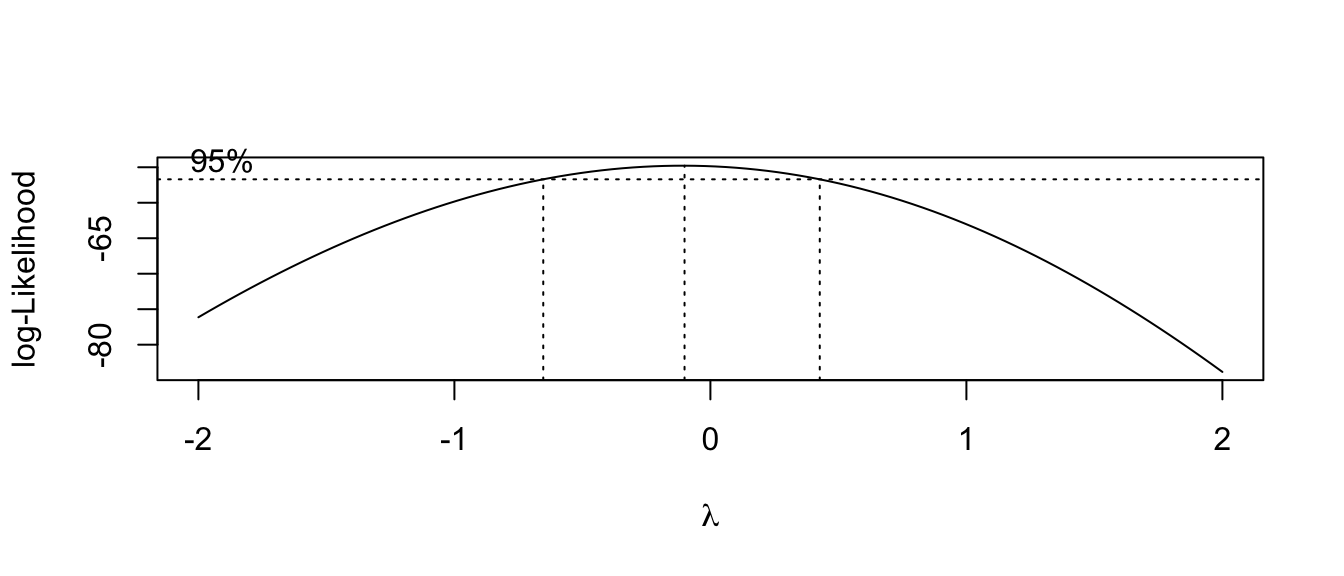
\includegraphics{Statistical_Methods_II_files/figure-latex/unnamed-chunk-172-1.pdf}

All of the line segments are close to parallel so, we don't expect the
interaction to be significant.

\begin{Shaded}
\begin{Highlighting}[]
\KeywordTok{anova}\NormalTok{( m4 )}
\end{Highlighting}
\end{Shaded}

\begin{verbatim}
## Analysis of Variance Table
## 
## Response: Yield
##           Df Sum Sq Mean Sq F value    Pr(>F)    
## Var        2 3996.1 1998.04 47.2443 2.048e-06 ***
## Pest       3 2227.5  742.49 17.5563 0.0001098 ***
## Var:Pest   6  456.9   76.15  1.8007 0.1816844    
## Residuals 12  507.5   42.29                      
## ---
## Signif. codes:  0 '***' 0.001 '**' 0.01 '*' 0.05 '.' 0.1 ' ' 1
\end{verbatim}

Examining the ANOVA table, we see that the interaction effect is not
significant and we will stay with simpler model
\texttt{Yield\textasciitilde{}Var+Pest}.

\subsection{Example - Warpbreaks}\label{example---warpbreaks}

This data set looks at the number of breaks that occur in two different
types of wool under three different levels of tension (low, medium, and
high). The fewer number of breaks, the better.

As always, the first thing we do is look at the data. In this case, it
looks like the number of breaks decreases with increasing tension and
perhaps wool B has fewer breaks than wool A.

\begin{Shaded}
\begin{Highlighting}[]
\KeywordTok{library}\NormalTok{(ggplot2)}
\KeywordTok{library}\NormalTok{(faraway)}
\KeywordTok{data}\NormalTok{(warpbreaks)}
\KeywordTok{ggplot}\NormalTok{(warpbreaks, }\KeywordTok{aes}\NormalTok{(}\DataTypeTok{x=}\NormalTok{tension, }\DataTypeTok{y=}\NormalTok{breaks, }\DataTypeTok{color=}\NormalTok{wool, }\DataTypeTok{shape=}\NormalTok{wool), }\DataTypeTok{size=}\DecValTok{2}\NormalTok{) +}\StringTok{ }
\StringTok{  }\KeywordTok{geom_boxplot}\NormalTok{() +}
\StringTok{  }\KeywordTok{geom_point}\NormalTok{(}\DataTypeTok{position=}\KeywordTok{position_dodge}\NormalTok{(}\DataTypeTok{width=}\NormalTok{.}\DecValTok{35}\NormalTok{)) }\CommentTok{# offset the wool groups }
\end{Highlighting}
\end{Shaded}

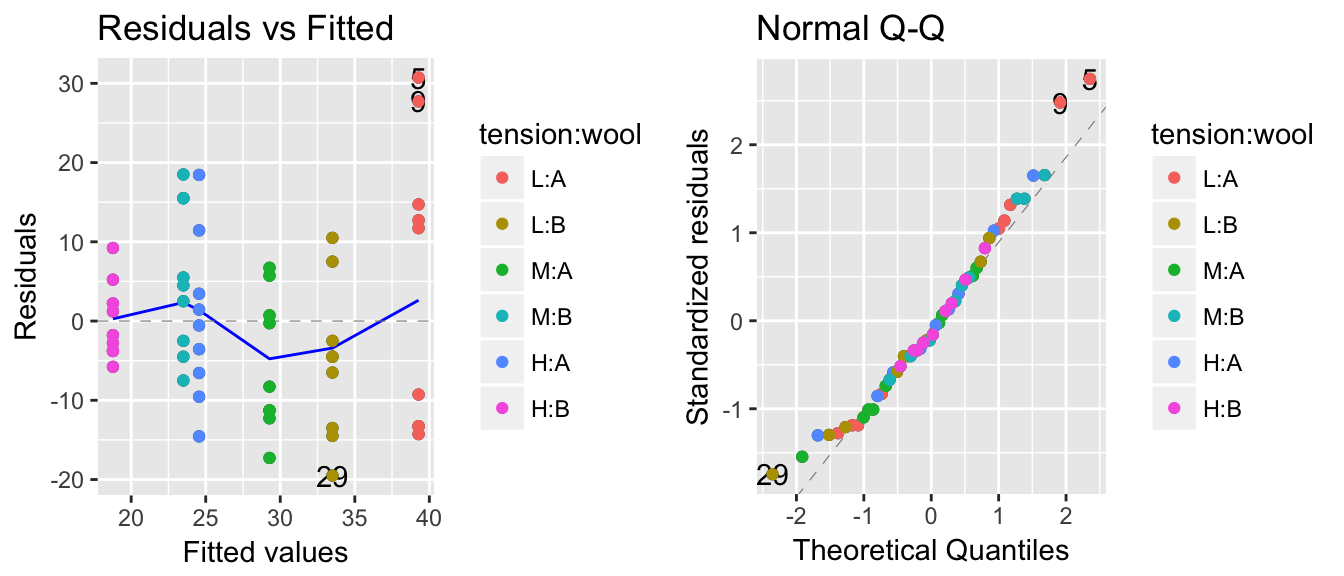
\includegraphics{Statistical_Methods_II_files/figure-latex/unnamed-chunk-174-1.pdf}

We next fit our linear model and examine the diagnostic plots.

\begin{Shaded}
\begin{Highlighting}[]
\NormalTok{model <-}\StringTok{ }\KeywordTok{lm}\NormalTok{(breaks ~}\StringTok{ }\NormalTok{tension +}\StringTok{ }\NormalTok{wool, }\DataTypeTok{data=}\NormalTok{warpbreaks)}
\KeywordTok{autoplot}\NormalTok{(model, }\DataTypeTok{which=}\KeywordTok{c}\NormalTok{(}\DecValTok{1}\NormalTok{,}\DecValTok{2}\NormalTok{))}
\end{Highlighting}
\end{Shaded}

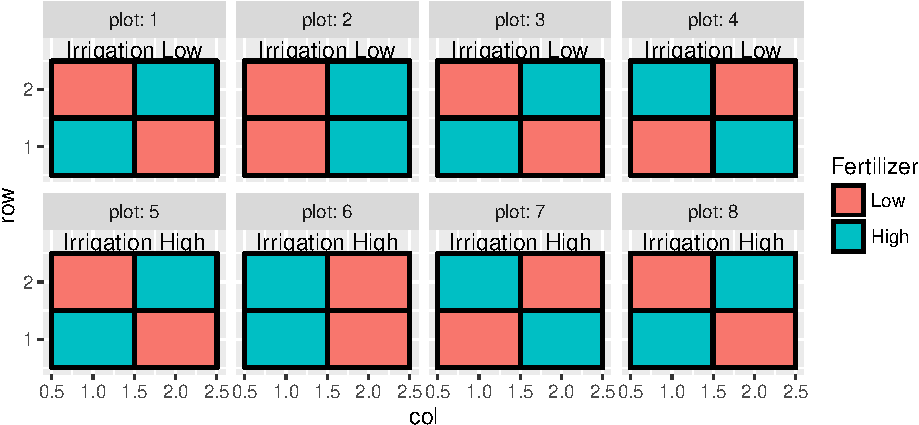
\includegraphics{Statistical_Methods_II_files/figure-latex/unnamed-chunk-175-1.pdf}

The residuals vs fitted values plot is a little worrisome and appears to
be an issue with non-constant variance, but the normality assumption
looks good. We'll check for a Box-Cox transformation next.

\begin{Shaded}
\begin{Highlighting}[]
\KeywordTok{boxcox}\NormalTok{(model)}
\end{Highlighting}
\end{Shaded}

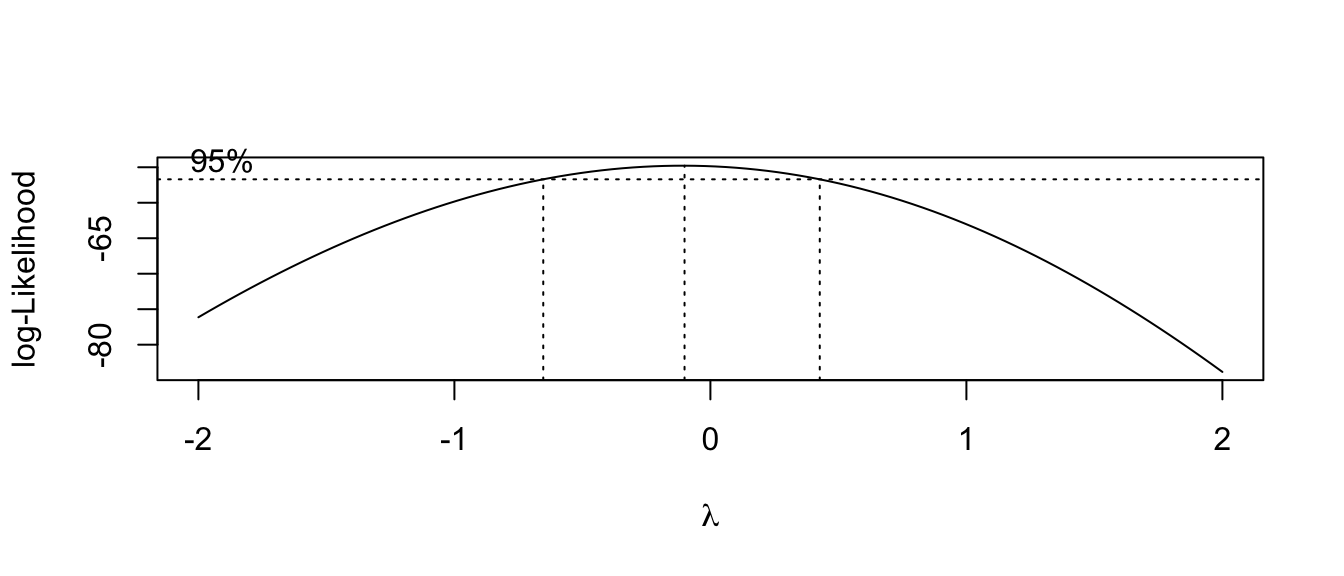
\includegraphics{Statistical_Methods_II_files/figure-latex/unnamed-chunk-176-1.pdf}

This suggests we should make a log transformation, though because the
confidence interval is quite wide we might consider if the increased
difficulty in interpretation makes sufficient progress towards making
the data meet the model assumptions.. The diagnostic plots of the
resulting model look better for the constant variance assumption, but
the normality is now a worse off. Because the Central Limit Theorem
helps deal with the normality question, I'd rather stabilize the
variance at the cost of the normality.

\begin{Shaded}
\begin{Highlighting}[]
\NormalTok{model}\FloatTok{.1} \NormalTok{<-}\StringTok{ }\KeywordTok{lm}\NormalTok{(}\KeywordTok{log}\NormalTok{(breaks) ~}\StringTok{ }\NormalTok{tension +}\StringTok{ }\NormalTok{wool, }\DataTypeTok{data=}\NormalTok{warpbreaks)}
\KeywordTok{autoplot}\NormalTok{(model}\FloatTok{.1}\NormalTok{, }\DataTypeTok{which=}\KeywordTok{c}\NormalTok{(}\DecValTok{1}\NormalTok{,}\DecValTok{2}\NormalTok{))}
\end{Highlighting}
\end{Shaded}

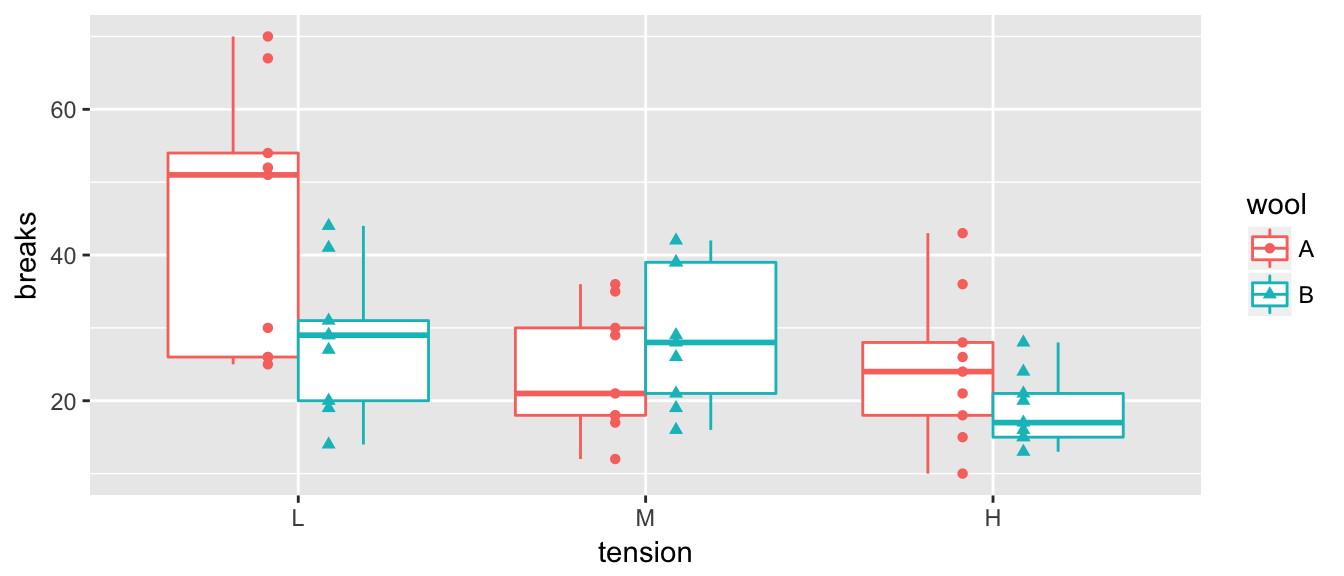
\includegraphics{Statistical_Methods_II_files/figure-latex/unnamed-chunk-177-1.pdf}

Next we'll fit the interaction model and check the diagnostic plots. The
diagnostic plots look good and this appears to be a legitimate model.

\begin{Shaded}
\begin{Highlighting}[]
\NormalTok{model}\FloatTok{.2} \NormalTok{<-}\StringTok{ }\KeywordTok{lm}\NormalTok{(}\KeywordTok{log}\NormalTok{(breaks) ~}\StringTok{ }\NormalTok{tension *}\StringTok{ }\NormalTok{wool, }\DataTypeTok{data=}\NormalTok{warpbreaks)}
\KeywordTok{autoplot}\NormalTok{(model}\FloatTok{.2}\NormalTok{, }\DataTypeTok{which=}\KeywordTok{c}\NormalTok{(}\DecValTok{1}\NormalTok{,}\DecValTok{2}\NormalTok{))}
\end{Highlighting}
\end{Shaded}

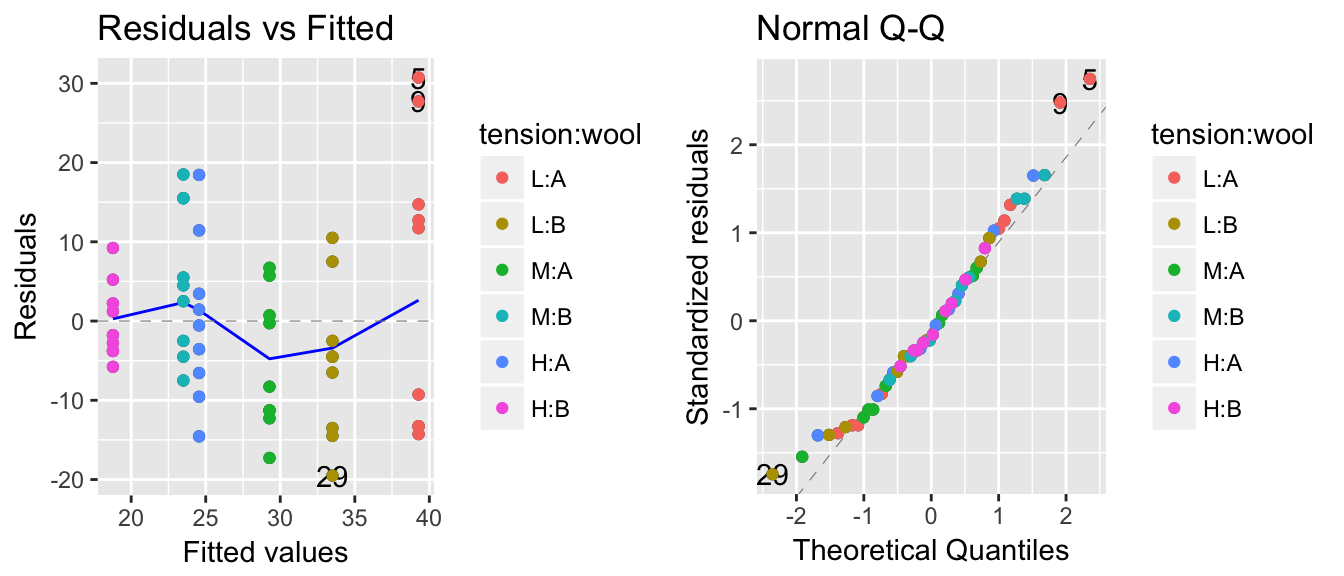
\includegraphics{Statistical_Methods_II_files/figure-latex/unnamed-chunk-178-1.pdf}

Then we'll do an F-test to see if it is a better model than the main
effects model. The p-value is marginally significant, so we'll keep the
interaction in the model, but recognize that it is a weak interaction.

\begin{Shaded}
\begin{Highlighting}[]
\KeywordTok{anova}\NormalTok{(model}\FloatTok{.1}\NormalTok{, model}\FloatTok{.2}\NormalTok{)}
\end{Highlighting}
\end{Shaded}

\begin{verbatim}
## Analysis of Variance Table
## 
## Model 1: log(breaks) ~ tension + wool
## Model 2: log(breaks) ~ tension * wool
##   Res.Df    RSS Df Sum of Sq      F  Pr(>F)  
## 1     50 7.6270                              
## 2     48 6.7138  2   0.91315 3.2642 0.04686 *
## ---
## Signif. codes:  0 '***' 0.001 '**' 0.01 '*' 0.05 '.' 0.1 ' ' 1
\end{verbatim}

Next we look at the effect of the interaction and the easiest way to do
this is to look at the interaction plot. This plot shows the raw data
and connects lines to the cell mean of each factor combination.

\begin{Shaded}
\begin{Highlighting}[]
\NormalTok{warpbreaks$logy.hat <-}\StringTok{ }\KeywordTok{predict}\NormalTok{(model}\FloatTok{.2}\NormalTok{)}
\KeywordTok{ggplot}\NormalTok{(warpbreaks, }\KeywordTok{aes}\NormalTok{(}\DataTypeTok{x=}\NormalTok{tension, }\DataTypeTok{y=}\KeywordTok{log}\NormalTok{(breaks), }\DataTypeTok{color=}\NormalTok{wool, }\DataTypeTok{shape=}\NormalTok{wool)) +}
\StringTok{  }\KeywordTok{geom_point}\NormalTok{() +}
\StringTok{  }\KeywordTok{geom_line}\NormalTok{(}\KeywordTok{aes}\NormalTok{(}\DataTypeTok{y=}\NormalTok{logy.hat, }\DataTypeTok{x=}\KeywordTok{as.integer}\NormalTok{(tension)))}
\end{Highlighting}
\end{Shaded}

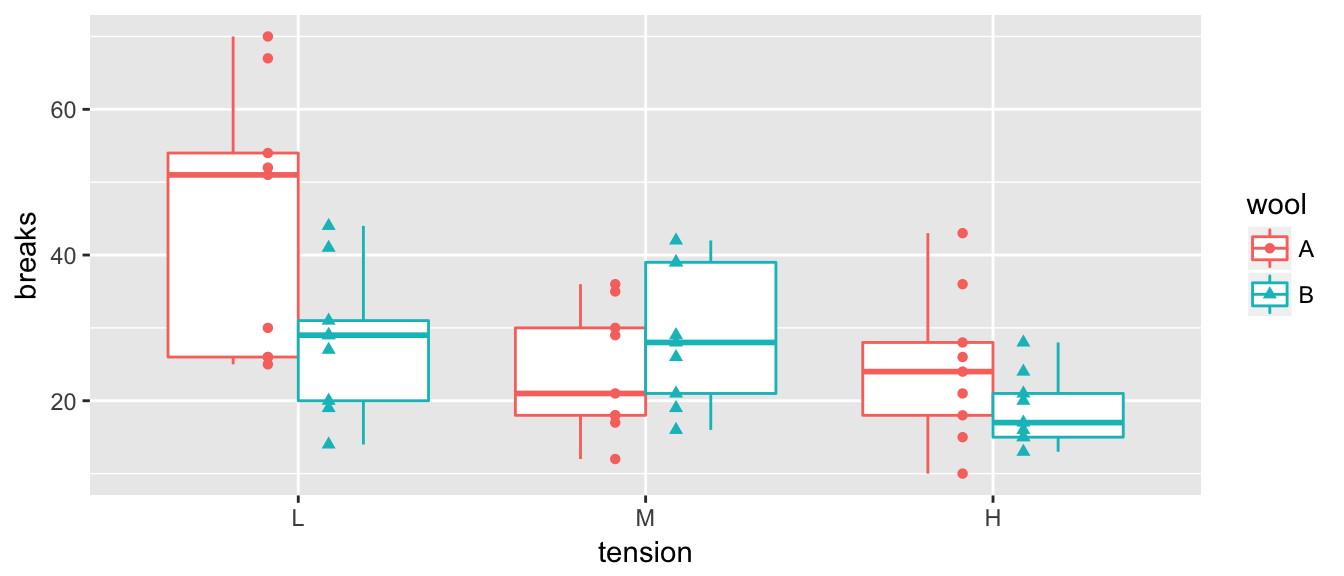
\includegraphics{Statistical_Methods_II_files/figure-latex/unnamed-chunk-180-1.pdf}

We can see that it appears that wool A has a decrease in breaks between
low and medium tension, while wool B has a decrease in breaks between
medium and high. It is actually quite difficult to see this interaction
when we examine the model coefficients.

\begin{Shaded}
\begin{Highlighting}[]
\KeywordTok{summary}\NormalTok{(model}\FloatTok{.2}\NormalTok{)}
\end{Highlighting}
\end{Shaded}

\begin{verbatim}
## 
## Call:
## lm(formula = log(breaks) ~ tension * wool, data = warpbreaks)
## 
## Residuals:
##      Min       1Q   Median       3Q      Max 
## -0.81504 -0.27885  0.04042  0.27319  0.64358 
## 
## Coefficients:
##                Estimate Std. Error t value Pr(>|t|)    
## (Intercept)      3.7179     0.1247  29.824  < 2e-16 ***
## tensionM        -0.6012     0.1763  -3.410  0.00133 ** 
## tensionH        -0.6003     0.1763  -3.405  0.00134 ** 
## woolB           -0.4356     0.1763  -2.471  0.01709 *  
## tensionM:woolB   0.6281     0.2493   2.519  0.01514 *  
## tensionH:woolB   0.2221     0.2493   0.891  0.37749    
## ---
## Signif. codes:  0 '***' 0.001 '**' 0.01 '*' 0.05 '.' 0.1 ' ' 1
## 
## Residual standard error: 0.374 on 48 degrees of freedom
## Multiple R-squared:  0.3363, Adjusted R-squared:  0.2672 
## F-statistic: 4.864 on 5 and 48 DF,  p-value: 0.001116
\end{verbatim}

To test if there is a statistically significant difference between
medium and high tensions for wool type B, we really need to test the
following hypothesis: \[\begin{aligned}
H_{0}:\;\left(\mu+\alpha_{2}+\beta_{2}+\left(\alpha\beta\right)_{22}\right)-\left(\mu+\alpha_{3}+\beta_{2}+\left(\alpha\beta\right)_{32}\right) & =   0 \\
H_{a}:\;\left(\mu+\alpha_{2}+\beta_{2}+\left(\alpha\beta\right)_{22}\right)-\left(\mu+\alpha_{3}+\beta_{2}+\left(\alpha\beta\right)_{32}\right) &\ne    0
\end{aligned}\]

This test reduces to testing if
\(\alpha_{2}-\alpha_{3}+\left(\alpha\beta\right)_{22}-\left(\alpha\beta\right)_{23}=0\).
Calculating this difference from the estimated values of the summery
table we have \(-.6012+.6003+.6281-.2221=0.4051\), we don't know if that
is significantly different than zero.

In the main effects model, we were able to read off the necessary test
using Tukey's HSD. Fortunately, we can do the same thing here. In this
case, we'll look at the interactions piece of the TukeyHSD command. In
this case, we find the test H:B - M:B in the last row of the
interactions.

\begin{Shaded}
\begin{Highlighting}[]
\KeywordTok{TukeyHSD}\NormalTok{( }\KeywordTok{aov}\NormalTok{(model}\FloatTok{.2}\NormalTok{) )}
\end{Highlighting}
\end{Shaded}

\begin{verbatim}
##   Tukey multiple comparisons of means
##     95% family-wise confidence level
## 
## Fit: aov(formula = model.2)
## 
## $tension
##           diff        lwr         upr     p adj
## M-L -0.2871237 -0.5886239  0.01437636 0.0649432
## H-L -0.4892747 -0.7907748 -0.18777463 0.0007948
## H-M -0.2021510 -0.5036511  0.09934912 0.2465032
## 
## $wool
##           diff        lwr        upr     p adj
## B-A -0.1521536 -0.3568127 0.05250558 0.1415114
## 
## $`tension:wool`
##                  diff        lwr         upr     p adj
## M:A-L:A -0.6011957092 -1.1244431 -0.07794828 0.0157632
## H:A-L:A -0.6003226799 -1.1235701 -0.07707525 0.0159794
## L:B-L:A -0.4355668365 -0.9588143  0.08768059 0.1534713
## M:B-L:A -0.4086186238 -0.9318661  0.11462881 0.2071300
## H:B-L:A -0.8137936293 -1.3370411 -0.29054620 0.0004035
## H:A-M:A  0.0008730293 -0.5223744  0.52412046 1.0000000
## L:B-M:A  0.1656288727 -0.3576186  0.68887630 0.9341161
## M:B-M:A  0.1925770854 -0.3306703  0.71582452 0.8820529
## H:B-M:A -0.2125979201 -0.7358454  0.31064951 0.8318529
## L:B-H:A  0.1647558434 -0.3584916  0.68800327 0.9354994
## M:B-H:A  0.1917040562 -0.3315434  0.71495149 0.8840239
## H:B-H:A -0.2134709494 -0.7367184  0.30977648 0.8294547
## M:B-L:B  0.0269482127 -0.4962992  0.55019564 0.9999876
## H:B-L:B -0.3782267929 -0.9014742  0.14502064 0.2822984
## H:B-M:B -0.4051750056 -0.9284224  0.11807242 0.2148594
\end{verbatim}

So TukeyHSD gives us all the tests comparing the cell means, but what
are those main effects testing? In the case where our experiment is
balanced with equal numbers of observations in each treatment cell, we
can interpret these differences as follows. Knowing that each cell in
our table has a different estimated mean, we could consider the average
of all the type A cells as the typical wool A. Likewise we could average
all the cell means for the wool B cells. Then we could look at the
difference between those two averages. In the balanced design, this is
equivalent to removing the tension term from the model and just looking
at the difference between the average log number of breaks.

Using TukeyHSD, we can see the wool effect difference between types B
and A is \(-0.1522\). We can calculate the mean number of log breaks for
each wool type and take the difference by the following:

\begin{Shaded}
\begin{Highlighting}[]
\NormalTok{warpbreaks %>%}\StringTok{ }
\StringTok{  }\KeywordTok{group_by}\NormalTok{(wool) %>%}\StringTok{ }
\StringTok{  }\KeywordTok{summarise}\NormalTok{( }\DataTypeTok{wool.means =} \KeywordTok{mean}\NormalTok{(}\KeywordTok{log}\NormalTok{(breaks)) ) %>%}
\StringTok{  }\KeywordTok{summarise}\NormalTok{( }\KeywordTok{diff}\NormalTok{(wool.means) )}
\end{Highlighting}
\end{Shaded}

\begin{verbatim}
## # A tibble: 1 x 1
##   `diff(wool.means)`
##                <dbl>
## 1         -0.1521536
\end{verbatim}

In the unbalanced case taking the average of the cell means produces a
different answer than taking the average of the data. It isn't clear
which is preferred and TukeyHSD produces a result that is between those
two methods.

\section{Exercises}\label{exercises-8}

\begin{enumerate}
\def\labelenumi{\arabic{enumi}.}
\tightlist
\item
  In the \texttt{faraway} package, the data set \texttt{rats} has data
  on a gruesome experiment that examined the time till death of 48 rats
  when they were subjected to three different types of poison
  administered in four different manners (which they called treatments).
  We are interested in assessing which poison works the fastest as well
  as which administration method is most effective.

  \begin{enumerate}
  \def\labelenumii{\alph{enumii}.}
  \tightlist
  \item
    Consider the interaction model which allows for a different effect
    of treatment for each poison type. Fit this model and examine the
    diagnostic plots. What stands out?
  \item
    Perform a Box-Cox analysis and perform the recommended
    transformation (with the realm of ``common'' transformations). Call
    the transformed variable \texttt{speed}.
  \item
    Fit the interaction model using the transformed response. Create a
    graph of data and the predicted values. Visually assess if you think
    the interaction is significant.
  \item
    Perform an appropriate statistical test to see if the interaction is
    statistically significant.
  \item
    What do you conclude about the poisons and treatment (application)
    types?
  \end{enumerate}
\item
  In the \texttt{faraway} package, the dataset \texttt{butterfat} has
  information about the the percent of the milk was butterfat (more is
  better) taken from \(n=100\) cows. There are \(5\) different breeds of
  cows and \(2\) different ages. We are interested in asessing if
  \texttt{Age} and \texttt{Breed} affect the butterfat content

  \begin{enumerate}
  \def\labelenumii{\alph{enumii}.}
  \tightlist
  \item
    Graph the data. Do you think an interaction model is justified?
  \item
    Perform an appropriate set of tests to select a model for predicting
    \texttt{Butterfat}.
  \item
    Discuss your findings.
  \end{enumerate}
\item
  In the \texttt{faraway} package, the dataset \texttt{alfalfa} has
  information from a study that examined the effect of seed innoculum,
  irrigation, and shade on alfalfa yield. This data has \(n=24\)
  observations.

  \begin{enumerate}
  \def\labelenumii{\alph{enumii}.}
  \tightlist
  \item
    Graph the data.
  \item
    Consider the main effects model with all three predictor variables.
    Examine the diagnostic plots and comment. Consider a Box-Cox
    transformation to your response (you might need to use
    \texttt{lambda\ =\ seq(-2,6,\ by=.01)} to see the whole curve). Make
    any transformation you feel is justified.
  \item
    Consider the model with \texttt{shade} and \texttt{inoculum} and the
    interaction between the two. Examine the anova table. Why does R
    complain that the fit is perfect? \emph{Hint: Think about the
    degrees of freedom of the model compared to the sample size.}
  \item
    Discuss your findings and the limitations of your investigation
    based on data.
  \end{enumerate}
\end{enumerate}

\chapter{Block Designs}\label{block-designs}

\begin{Shaded}
\begin{Highlighting}[]
\CommentTok{# packages for this chapter}
\KeywordTok{library}\NormalTok{(tidyverse)    }\CommentTok{# ggplot2, dplyr, etc...}
\KeywordTok{library}\NormalTok{(multcompView) }\CommentTok{# TukeyLetters stuff}
\KeywordTok{library}\NormalTok{(devtools)}
\CommentTok{#install_github('dereksonderegger/dsData')  # some datasets I've made up; only install once...}
\KeywordTok{library}\NormalTok{(dsData)}
\KeywordTok{library}\NormalTok{(faraway)}
\KeywordTok{library}\NormalTok{(MASS)         }\CommentTok{# for the oats dataset}
\end{Highlighting}
\end{Shaded}

Often there are covariates in the experimental units that are known to
affect the response variable and must be taken into account. Ideally an
experimenter can group the experimental units into blocks where the
within block variance is small, but the block to block variability is
large. For example, in testing a drug to prevent heart disease, we know
that gender, age, and exercise levels play a large role. We should
partition our study participants into gender, age, and exercise groups
and then randomly assign the treatment (placebo vs drug) within the
group. This will ensure that we do not have a gender, age, and exercise
group that has all placebo observations.

Often blocking variables are not the variables that we are primarily
interested in, but must nevertheless be considered. We call these
nuisance variables. We already know how to deal with these variables by
adding them to the model, but there are experimental designs where we
must be careful because the experimental treatments are \emph{nested}.

Example 1. An agricultural field study has three fields in which the
researchers will evaluate the quality of three different varieties of
barley. Due to how they harvest the barley, we can only create a maximum
of three plots in each field. In this example we will block on field
since there might be differences in soil type, drainage, etc from field
to field. In each field, we will plant all three varieties so that we
can tell the difference between varieties without the block effect of
field confounding our inference. In this example, the varieties are
nested within the fields.

\begin{longtable}[]{@{}llll@{}}
\toprule
\begin{minipage}[b]{0.18\columnwidth}\raggedright\strut
\strut
\end{minipage} & \begin{minipage}[b]{0.17\columnwidth}\raggedright\strut
Field 1\strut
\end{minipage} & \begin{minipage}[b]{0.16\columnwidth}\raggedright\strut
Field 2\strut
\end{minipage} & \begin{minipage}[b]{0.16\columnwidth}\raggedright\strut
Field 3\strut
\end{minipage}\tabularnewline
\midrule
\endhead
\begin{minipage}[t]{0.18\columnwidth}\raggedright\strut
\textbf{Plot 1}\strut
\end{minipage} & \begin{minipage}[t]{0.17\columnwidth}\raggedright\strut
Variety A\strut
\end{minipage} & \begin{minipage}[t]{0.16\columnwidth}\raggedright\strut
Variety C\strut
\end{minipage} & \begin{minipage}[t]{0.16\columnwidth}\raggedright\strut
Variety B\strut
\end{minipage}\tabularnewline
\begin{minipage}[t]{0.18\columnwidth}\raggedright\strut
\textbf{Plot 2}\strut
\end{minipage} & \begin{minipage}[t]{0.17\columnwidth}\raggedright\strut
Variety B\strut
\end{minipage} & \begin{minipage}[t]{0.16\columnwidth}\raggedright\strut
Variety A\strut
\end{minipage} & \begin{minipage}[t]{0.16\columnwidth}\raggedright\strut
Variety C\strut
\end{minipage}\tabularnewline
\begin{minipage}[t]{0.18\columnwidth}\raggedright\strut
\textbf{Plot 3}\strut
\end{minipage} & \begin{minipage}[t]{0.17\columnwidth}\raggedright\strut
Variety C\strut
\end{minipage} & \begin{minipage}[t]{0.16\columnwidth}\raggedright\strut
Variety B\strut
\end{minipage} & \begin{minipage}[t]{0.16\columnwidth}\raggedright\strut
Variety A\strut
\end{minipage}\tabularnewline
\bottomrule
\end{longtable}

Example 2. We are interested in how a mouse responds to five different
materials inserted into subcutaneous tissue to evaluate the materials'
use in medicine. Each mouse can have a maximum of 3 insertions. Here we
will block on the individual mice because even lab mice have individual
variation. We actually are not interested in estimating the effect of
the mice because they aren't really of interest, but the mouse block
effect should be accounted for before we make any inferences about the
materials. Notice that if we only have one insertion per mouse, then the
mouse effect will be confounded with materials.

\section{Randomized Complete Block Design
(RCBD)}\label{randomized-complete-block-design-rcbd}

The dataset oatvar in the faraway library contains information about an
experiment on eight different varieties of oats. The area in which the
experiment was done had some systematic variability and the researchers
divided the area up into five different blocks in which they felt the
area inside a block was uniform while acknowledging that some blocks are
likely superior to others for growing crops. Within each block, the
researchers created eight plots and randomly assigned a variety to a
plot. This type of design is called a Randomized Complete Block Design
(RCBD) because each block contains all possible levels of the factor of
primary interest.

\begin{Shaded}
\begin{Highlighting}[]
\KeywordTok{data}\NormalTok{(oatvar)}
\KeywordTok{ggplot}\NormalTok{(oatvar, }\KeywordTok{aes}\NormalTok{(}\DataTypeTok{y=}\NormalTok{yield, }\DataTypeTok{x=}\NormalTok{block, }\DataTypeTok{color=}\NormalTok{variety)) +}\StringTok{ }
\StringTok{    }\KeywordTok{geom_point}\NormalTok{(}\DataTypeTok{size=}\DecValTok{5}\NormalTok{) +}
\StringTok{    }\KeywordTok{geom_line}\NormalTok{(}\KeywordTok{aes}\NormalTok{(}\DataTypeTok{x=}\KeywordTok{as.integer}\NormalTok{(block))) }\CommentTok{# connect the dots}
\end{Highlighting}
\end{Shaded}

\includegraphics{Statistical_Methods_II_files/figure-latex/unnamed-chunk-186-1.pdf}

While there is one unusual observation in block IV, there doesn't appear
to be a blatant interaction. We will consider the interaction shortly.
For the main effects model of yield \textasciitilde{} block + variety we
have \(p=12\) parameters and \(28\) residual degrees of freedom because
\[\begin{aligned}
  df_\epsilon   &=  n-p \\
        &=  n-\left(1+\left[\left(I-1\right)+\left(J-1\right)\right]\right) \\
        &=  n-\left(1+\left[\left(5-1\right)+\left(8-1\right)\right]\right) \\
        &=  n-12 \\
        &=  28
 \end{aligned}\]

\begin{Shaded}
\begin{Highlighting}[]
\NormalTok{m1 <-}\StringTok{ }\KeywordTok{lm}\NormalTok{( yield ~}\StringTok{ }\NormalTok{block +}\StringTok{ }\NormalTok{variety, }\DataTypeTok{data=}\NormalTok{oatvar)}
\KeywordTok{anova}\NormalTok{(m1)}
\end{Highlighting}
\end{Shaded}

\begin{verbatim}
## Analysis of Variance Table
## 
## Response: yield
##           Df Sum Sq Mean Sq F value    Pr(>F)    
## block      4  33396  8348.9  6.2449  0.001008 ** 
## variety    7  77524 11074.8  8.2839 1.804e-05 ***
## Residuals 28  37433  1336.9                      
## ---
## Signif. codes:  0 '***' 0.001 '**' 0.01 '*' 0.05 '.' 0.1 ' ' 1
\end{verbatim}

\begin{Shaded}
\begin{Highlighting}[]
\CommentTok{# plot(m1)      # check diagnostic plots - they are fine...}
\end{Highlighting}
\end{Shaded}

Because this is an orthogonal design, the sums of squares doesn't change
regardless of which order we add the factors, but if we remove one or
two observations, they would.

In determining the significance of \texttt{variety} the above F-value
and p-value is correct. We have 40 observations (5 per variety), and
after accounting for the model structure (including the extraneous
blocking variable), we have \(28\) residual degrees of freedom.

But the F-value and p-value for testing if \texttt{block} is significant
is wrong! Imagine that variety didn't matter we just have 8 replicate
samples per block, but these aren't true replicates, they are what is
called \emph{pseudoreplicates}. Imagine taking a sample of \(n=3\)
people and observing their height at 1000 different points in time
during the day. You don't have 3000 data points for estimating the mean
height in the population, you have 3. Unless we account for the this,
the inference for the block variable is wrong.

\begin{Shaded}
\begin{Highlighting}[]
\NormalTok{m3 <-}\StringTok{ }\KeywordTok{aov}\NormalTok{( yield ~}\StringTok{ }\NormalTok{block +}\StringTok{ }\NormalTok{variety +}\StringTok{ }\KeywordTok{Error}\NormalTok{(block), }\DataTypeTok{data=}\NormalTok{oatvar)}
\KeywordTok{summary}\NormalTok{(m3)}
\end{Highlighting}
\end{Shaded}

\begin{verbatim}
## 
## Error: block
##       Df Sum Sq Mean Sq
## block  4  33396    8349
## 
## Error: Within
##           Df Sum Sq Mean Sq F value  Pr(>F)    
## variety    7  77524   11075   8.284 1.8e-05 ***
## Residuals 28  37433    1337                    
## ---
## Signif. codes:  0 '***' 0.001 '**' 0.01 '*' 0.05 '.' 0.1 ' ' 1
\end{verbatim}

Fortunately in this case, we don't care about the blocking variable and
including it in the model was simply guarding us in case there was a
difference, but I wasn't interested in estimating it. If the only
covariate I care about is the most deeply nested effect, then I can do
my usual analysis and recognize the p-values for the blocking variable
is wrong, but I don't care about it.

\begin{Shaded}
\begin{Highlighting}[]
\CommentTok{#' Create a data frame with significant groupings }
\CommentTok{#'}
\CommentTok{#' This function runs TukeyHSD on the input model and then creates a data frame}
\CommentTok{#' with a column for the factor and a second for the Significance Group}
\CommentTok{#' }
\CommentTok{#' @param model The output of a lm() or aov() call that can be coerced to an aov object.}
\CommentTok{#' @param variable The variable of interest.}
\CommentTok{#' @output A data frame with a column for factor and another for the signicance group.}
\NormalTok{make_TukeyHSD_letters <-}\StringTok{ }\NormalTok{function(model, variable)\{ }
  \NormalTok{Tukey <-}\StringTok{ }\KeywordTok{TukeyHSD}\NormalTok{(}\KeywordTok{aov}\NormalTok{(model))[[variable]]}
  \NormalTok{temp <-}\StringTok{ }\NormalTok{Tukey[,}\StringTok{'p adj'}\NormalTok{] %>%}
\StringTok{    }\KeywordTok{vec2mat}\NormalTok{() %>%}
\StringTok{    }\KeywordTok{multcompLetters}\NormalTok{()}
  \NormalTok{out <-}\StringTok{ }\KeywordTok{data.frame}\NormalTok{(}\DataTypeTok{group =} \KeywordTok{names}\NormalTok{(temp$Letters), }\DataTypeTok{SigGroup=}\NormalTok{temp$Letters)}
  \KeywordTok{colnames}\NormalTok{(out)[}\DecValTok{1}\NormalTok{] <-}\StringTok{ }\NormalTok{variable}
  \NormalTok{out}
\NormalTok{\}  }
\end{Highlighting}
\end{Shaded}

\begin{Shaded}
\begin{Highlighting}[]
\CommentTok{# Ignore any p-values regarding block, but I'm happy with the analysis for variety}
\NormalTok{oatvar <-}\StringTok{ }\NormalTok{oatvar %>%}
\StringTok{  }\KeywordTok{left_join}\NormalTok{( }\KeywordTok{make_TukeyHSD_letters}\NormalTok{( m1, }\StringTok{'variety'}\NormalTok{) )}
\end{Highlighting}
\end{Shaded}

\begin{verbatim}
## Joining, by = "variety"
\end{verbatim}

\begin{Shaded}
\begin{Highlighting}[]
\KeywordTok{ggplot}\NormalTok{(oatvar, }\KeywordTok{aes}\NormalTok{(}\DataTypeTok{x=}\NormalTok{variety, }\DataTypeTok{y=}\NormalTok{yield)) +}
\StringTok{  }\KeywordTok{geom_boxplot}\NormalTok{() +}
\StringTok{  }\KeywordTok{geom_text}\NormalTok{( }\KeywordTok{aes}\NormalTok{(}\DataTypeTok{label=}\NormalTok{SigGroup), }\DataTypeTok{y=}\DecValTok{505}\NormalTok{) +}
\StringTok{  }\KeywordTok{scale_y_continuous}\NormalTok{(}\DataTypeTok{limits=}\KeywordTok{c}\NormalTok{(}\DecValTok{200}\NormalTok{, }\DecValTok{510}\NormalTok{))  }\CommentTok{# give me some room for letters}
\end{Highlighting}
\end{Shaded}

\includegraphics{Statistical_Methods_II_files/figure-latex/unnamed-chunk-190-1.pdf}

\section{Split-plot designs}\label{split-plot-designs}

There are plenty of experimental designs where we have levels of
treatments nested within each other for practical reasons. The
literature often gives the example of an agriculture experiment where we
investigate the effect of irrigation and fertilizer on the yield of a
crop. However because our irrigation system can't be fine-tuned, we have
plots with different irrigation levels and within each plot we have
perhaps four subplots that have the fertilizer treatment.

\includegraphics{Statistical_Methods_II_files/figure-latex/unnamed-chunk-192-1.pdf}

So all together we have 8 plots, and 32 subplots. When I analyze the
fertilizer, I have 32 experimental units (the thing I have applied my
treatment to), but when analyzing the effect of irrigation, I only have
8 experimental units.

I like to think of this set up as having some lurking variables that act
at the plot level (changes in aspect, maybe something related to what
was planted prior) and some lurking variables that act on a local
subplot scale (maybe variation in clay/silt/sand ratios). So even after
I account for Irrigation and Fertilizer treatments, observations within
a plot will be more similar to each other than observations in two
different plots.

We can think about doing two separate analyses, one for the effect of
irrigation, and another for the effect of the fertilizer.

\begin{Shaded}
\begin{Highlighting}[]
\CommentTok{# To analyze Irrigation, average over the subplots first...}
\NormalTok{Irrigation.data <-}\StringTok{   }\NormalTok{AgData %>%}\StringTok{ }
\StringTok{  }\KeywordTok{group_by}\NormalTok{(plot, Irrigation) %>%}
\StringTok{  }\KeywordTok{summarise}\NormalTok{( }\DataTypeTok{yield =} \KeywordTok{mean}\NormalTok{(yield)) }

\CommentTok{# Now do a standard analysis. I use the aov() command instead of lm()}
\CommentTok{# because we will shortly do something very tricky that can only be}
\CommentTok{# done with aov(). For the most part, everything is }
\CommentTok{# identical from what you are used to.}
\NormalTok{m <-}\StringTok{ }\KeywordTok{aov}\NormalTok{( yield ~}\StringTok{ }\NormalTok{Irrigation, }\DataTypeTok{data=}\KeywordTok{data.frame}\NormalTok{(Irrigation.data) )}
\KeywordTok{anova}\NormalTok{(m)}
\end{Highlighting}
\end{Shaded}

\begin{verbatim}
## Analysis of Variance Table
## 
## Response: yield
##            Df Sum Sq Mean Sq F value Pr(>F)
## Irrigation  1 26.064 26.0645  3.4281 0.1136
## Residuals   6 45.619  7.6032
\end{verbatim}

In this case we see that we have insufficient evidence to conclude that
the observed difference between the Irrigation levels could not be due
to random chance.

Next we can do the appropriate analysis for the fertilizer, recognizing
that all the p-values for the plot effects are nonsense and should be
ignored.

\begin{Shaded}
\begin{Highlighting}[]
\NormalTok{m <-}\StringTok{ }\KeywordTok{aov}\NormalTok{( yield ~}\StringTok{ }\NormalTok{plot +}\StringTok{ }\NormalTok{Fertilizer, }\DataTypeTok{data=}\NormalTok{AgData )}
\KeywordTok{summary}\NormalTok{(m)}
\end{Highlighting}
\end{Shaded}

\begin{verbatim}
##             Df Sum Sq Mean Sq F value Pr(>F)  
## plot         7 286.73   40.96   3.202 0.0161 *
## Fertilizer   1   5.05    5.05   0.395 0.5360  
## Residuals   23 294.22   12.79                 
## ---
## Signif. codes:  0 '***' 0.001 '**' 0.01 '*' 0.05 '.' 0.1 ' ' 1
\end{verbatim}

Ideally I wouldn't have to do the averaging over the nested observations
and we would like to not have the misleading p-values for the plots. To
do this, we only have to specify the nesting of the error terms and R
will figure out the appropriate degrees of freedom for the covariates.

\begin{Shaded}
\begin{Highlighting}[]
\CommentTok{# To do this right, we have to abandon the general lm() command and use the more}
\CommentTok{# specialized aov() command.  The Error() part of the formula allows me to nest}
\CommentTok{# the error terms and allow us to do the correct analysis. The order of these is}
\CommentTok{# to start with the largest/highest level and then work down the nesting.}
\NormalTok{m2 <-}\StringTok{ }\KeywordTok{aov}\NormalTok{( yield ~}\StringTok{ }\NormalTok{Irrigation +}\StringTok{ }\NormalTok{Fertilizer +}\StringTok{ }\KeywordTok{Error}\NormalTok{(plot/subplot), }\DataTypeTok{data=}\NormalTok{AgData )}
\KeywordTok{summary}\NormalTok{(m2)}
\end{Highlighting}
\end{Shaded}

\begin{verbatim}
## 
## Error: plot
##            Df Sum Sq Mean Sq F value Pr(>F)
## Irrigation  1  104.3  104.26   3.428  0.114
## Residuals   6  182.5   30.41               
## 
## Error: plot:subplot
##            Df Sum Sq Mean Sq F value Pr(>F)
## Fertilizer  1   5.05   5.049   0.395  0.536
## Residuals  23 294.22  12.792
\end{verbatim}

In the output, we see that the ANOVA table row for the Fertilizer is the
same for both analyses, but the sums-of-squares for Irrigation are
different between the two analyses (because of the averaging) while the
F and p values are the same between the two analyses.

What would have happened if we had performed the analysis incorrectly
and had too many degrees of freedom for the Irrigation test?

\begin{Shaded}
\begin{Highlighting}[]
\NormalTok{bad.model <-}\StringTok{ }\KeywordTok{aov}\NormalTok{( yield ~}\StringTok{ }\NormalTok{Irrigation +}\StringTok{ }\NormalTok{Fertilizer, }\DataTypeTok{data=}\NormalTok{AgData)}
\KeywordTok{anova}\NormalTok{(bad.model)}
\end{Highlighting}
\end{Shaded}

\begin{verbatim}
## Analysis of Variance Table
## 
## Response: yield
##            Df Sum Sq Mean Sq F value  Pr(>F)  
## Irrigation  1 104.26 104.258  6.3426 0.01756 *
## Fertilizer  1   5.05   5.049  0.3071 0.58369  
## Residuals  29 476.69  16.438                  
## ---
## Signif. codes:  0 '***' 0.001 '**' 0.01 '*' 0.05 '.' 0.1 ' ' 1
\end{verbatim}

In this case we would have concluded that we had statistically
significant evidence to conclude the Irrigation levels are different.
Notice that the sums-of-squares in this \textbf{wrong} analysis match up
with the sums-of-squares in the correct design and the only difference
is that when we figure out the sum-of-squares for the residuals we split
that into different pools. \[\begin{aligned}
  RSS_{total} &= RSS_{Fertilizer} + RSS_{Irrigation} \\
        304.0 &= 129.6 + 174.4
  \end{aligned}\]

When we want to infer if the amount of noise explained by adding
Irrigation or Fertilizer is sufficiently large to justify their
inclusion into the model, we compare the sum-of-squares value to the RSS
but now we have to use the appropriate pool.

\begin{center}\rule{0.5\linewidth}{\linethickness}\end{center}

A second example of a slightly more complex split plot is given in the
package \texttt{MASS} under the dataset \texttt{oats}. From the help
file the data describes the following experiment:

\begin{verbatim}
The yield of oats from a split-plot field trial using three varieties and 
four levels of manurial treatment. The experiment was laid out in 6 blocks 
of 3 main plots, each split into 4 sub-plots. The varieties were applied to 
the main plots and the manurial treatments to the sub-plots.
\end{verbatim}

This is a lot to digest so lets unpack it. First we have 6 blocks and
we'll replicate the exact same experiment in each block. Within a block,
we'll split it into three sections, which we'll call plots (within the
block). Finally within each plot, we'll have 4 subplots.

We have 3 varieties of oats, and 4 levels of fertilizer (manure). To
each set of 3 plots, we'll randomly assign the 3 varieties, and to each
set of subplots, we'll assign the fertilizers.

One issue that makes this issue confusing for students is that most
texts get lazy and don't define the blocks, plots, and sub-plots when
there are no replicates in a particular level. I prefer to be clear
about defining those so.

\begin{Shaded}
\begin{Highlighting}[]
\KeywordTok{data}\NormalTok{(oats)}
\NormalTok{oats <-}\StringTok{ }\NormalTok{oats %>%}\StringTok{ }\KeywordTok{mutate}\NormalTok{(}
  \DataTypeTok{Nf =} \KeywordTok{ordered}\NormalTok{(N, }\DataTypeTok{levels =} \KeywordTok{sort}\NormalTok{(}\KeywordTok{levels}\NormalTok{(N))),  }\CommentTok{# make manure an ordered factor}
  \DataTypeTok{plot =} \KeywordTok{as.integer}\NormalTok{(V),                       }\CommentTok{# plot}
  \DataTypeTok{subplot =} \KeywordTok{as.integer}\NormalTok{(Nf))                   }\CommentTok{# sub-plot}
\end{Highlighting}
\end{Shaded}

As always we first create a graph to examine the data

\begin{Shaded}
\begin{Highlighting}[]
\KeywordTok{ggplot}\NormalTok{(oats, }\KeywordTok{aes}\NormalTok{(}\DataTypeTok{x=}\NormalTok{Nf, }\DataTypeTok{y=}\NormalTok{Y, }\DataTypeTok{color=}\NormalTok{V)) +}
\StringTok{  }\KeywordTok{facet_wrap}\NormalTok{( ~}\StringTok{ }\NormalTok{B, }\DataTypeTok{ncol=}\DecValTok{3}\NormalTok{) +}
\StringTok{  }\KeywordTok{geom_point}\NormalTok{() +}
\StringTok{  }\KeywordTok{geom_line}\NormalTok{(}\KeywordTok{aes}\NormalTok{(}\DataTypeTok{x=}\KeywordTok{as.integer}\NormalTok{(Nf)))}
\end{Highlighting}
\end{Shaded}

\includegraphics{Statistical_Methods_II_files/figure-latex/unnamed-chunk-198-1.pdf}

This graph also makes me think that variety doesn't matter and it is
unlikely that there an interaction between oat variety and fertilizer
level, but we should check.

\begin{Shaded}
\begin{Highlighting}[]
\CommentTok{#  What makes sense to me}
\CommentTok{# m.c <- aov( Y ~ V * Nf + Error(B/plot/subplot), data=oats)}
\end{Highlighting}
\end{Shaded}

Unfortunately the above model isn't correct because R isn't smart enough
to understand that the levels of plot and subplot are exact matches to
the Variety and Fertilizer levels. As a result if I defined the model
above, the degrees of freedom will be all wrong because there is too
much nesting. So we have to be smart enough to recognize that plot and
subplot are actually Variety and Fertilizer.

\begin{Shaded}
\begin{Highlighting}[]
\NormalTok{m.c <-}\StringTok{ }\KeywordTok{aov}\NormalTok{( Y ~}\StringTok{ }\NormalTok{V *}\StringTok{ }\NormalTok{Nf +}\StringTok{ }\KeywordTok{Error}\NormalTok{(B/V/Nf), }\DataTypeTok{data=}\NormalTok{oats)}
\KeywordTok{summary}\NormalTok{(m.c)}
\end{Highlighting}
\end{Shaded}

\begin{verbatim}
## 
## Error: B
##           Df Sum Sq Mean Sq F value Pr(>F)
## Residuals  5  15875    3175               
## 
## Error: B:V
##           Df Sum Sq Mean Sq F value Pr(>F)
## V          2   1786   893.2   1.485  0.272
## Residuals 10   6013   601.3               
## 
## Error: B:V:Nf
##           Df Sum Sq Mean Sq F value   Pr(>F)    
## Nf         3  20020    6673  37.686 2.46e-12 ***
## V:Nf       6    322      54   0.303    0.932    
## Residuals 45   7969     177                     
## ---
## Signif. codes:  0 '***' 0.001 '**' 0.01 '*' 0.05 '.' 0.1 ' ' 1
\end{verbatim}

Sure enough the interaction term is not significant. We next consider
the Variety term.

\begin{Shaded}
\begin{Highlighting}[]
\NormalTok{m.s <-}\StringTok{ }\KeywordTok{aov}\NormalTok{( Y ~}\StringTok{ }\NormalTok{V +}\StringTok{ }\NormalTok{Nf +}\StringTok{ }\KeywordTok{Error}\NormalTok{(B/V/Nf), }\DataTypeTok{data=}\NormalTok{oats)}
\KeywordTok{summary}\NormalTok{(m.s)}
\end{Highlighting}
\end{Shaded}

\begin{verbatim}
## 
## Error: B
##           Df Sum Sq Mean Sq F value Pr(>F)
## Residuals  5  15875    3175               
## 
## Error: B:V
##           Df Sum Sq Mean Sq F value Pr(>F)
## V          2   1786   893.2   1.485  0.272
## Residuals 10   6013   601.3               
## 
## Error: B:V:Nf
##           Df Sum Sq Mean Sq F value   Pr(>F)    
## Nf         3  20020    6673   41.05 1.23e-13 ***
## Residuals 51   8291     163                     
## ---
## Signif. codes:  0 '***' 0.001 '**' 0.01 '*' 0.05 '.' 0.1 ' ' 1
\end{verbatim}

We conclude by noticing that the Variety does not matter, but that the
fertilizer level is quite significant.

\begin{center}\rule{0.5\linewidth}{\linethickness}\end{center}

There are many other types of designs out there. For example you might
have 5 levels of a factor, but when you split your block into plots, you
can only create 3 plots. So not every block will have every level of the
factor. This is called \emph{Randomized Incomplete Block Designs}
(RIBD).

You might have a design where you apply even more levels of nesting.
Suppose you have a green house study where you have rooms where you can
apply a temperature treatment, within the room you have four tables and
can apply a light treatment to each table. Finally within each table you
can have four trays where can apply a soil treatment to each tray. This
is a continuation of the split-plot design and by extending the nesting
we can develop \emph{split-split-plot} and \emph{split-split-split-plot}
designs.

You might have 7 covariates each with two levels (High, Low) and you
want to investigate how these influence your response but also allow for
second and third order interactions. If you looked at every treatment
combination you'd have \(2^7=128\) different treatment combinations and
perhaps you only have the budget for a sample of \(n=32\). How should
you design your experiment? This question is addressed by
\emph{fractional factorial} designs.

If your research interests involve designing experiments such as these,
you should consider taking an Experimental design course.

\section{Exercises}\label{exercises-9}

\begin{enumerate}
\def\labelenumi{\arabic{enumi}.}
\tightlist
\item
  ???
\item
  ???
\item
  ???
\end{enumerate}

\chapter{Mixed Effects Models}\label{mixed-effects-models}

\begin{Shaded}
\begin{Highlighting}[]
\KeywordTok{library}\NormalTok{(faraway)}
\KeywordTok{library}\NormalTok{(MASS)}
\KeywordTok{library}\NormalTok{(lme4)}
\KeywordTok{library}\NormalTok{(tidyverse)}
\KeywordTok{library}\NormalTok{(lsmeans)}
\KeywordTok{library}\NormalTok{(multcompView)}
\KeywordTok{library}\NormalTok{(car)}
\KeywordTok{library}\NormalTok{(stringr)}
\CommentTok{# library(devtools)}
\CommentTok{# install_github('dereksonderegger/dsData')  # some datasets I've made up; only install once...}
\KeywordTok{library}\NormalTok{(dsData)}
\KeywordTok{library}\NormalTok{(pander)}
\end{Highlighting}
\end{Shaded}

The assumption of independent observations is often not supported and
dependent data arises in a wide variety of situations. The dependency
structure could be very simple such as rabbits within a litter being
correlated and the litters being independent. More complex hierarchies
of correlation are possible. For example we might expect voters in a
particular part of town (called a precinct) to vote similarly, and
particular districts in a state tend to vote similarly as well, which
might result in a precinct / district / state hierarchy of correlation.

Many of the designs mentioned in the Block Designs section could be
similarly modeled using Mixed Effects Models. In many respects, the
random effects structure provides a more flexible framework to consider
many of the traditional experimental designs as well as many
non-traditional designs with the benefit of more easily assessing
variability at each hierarchical level.

Mixed effects models combine what we call ``fixed'' and ``random''
effects.

\begin{longtable}[]{@{}ll@{}}
\toprule
\begin{minipage}[t]{0.26\columnwidth}\raggedright\strut
\textbf{Fixed effects}\strut
\end{minipage} & \begin{minipage}[t]{0.68\columnwidth}\raggedright\strut
Unknown constants that we wish to estimate from the model and could be
similarly estimated in subsequent experimentation. The research is
interested in these particular levels.\strut
\end{minipage}\tabularnewline
\begin{minipage}[t]{0.26\columnwidth}\raggedright\strut
\textbf{Random effects}\strut
\end{minipage} & \begin{minipage}[t]{0.68\columnwidth}\raggedright\strut
Random variables sampled from a population which cannot be observed in
subsequent experimentation. The research is not interested in these
particular levels, but rather how the levels vary from sample to
sample.\strut
\end{minipage}\tabularnewline
\bottomrule
\end{longtable}

For example, in a rabbit study that examined the effect of diet on the
growth of domestic rabbits and we had 10 litters of rabbits and used the
3 most similar from each litter to test 6 different diets. Here, the 6
different diets are fixed effects because they are not randomly selected
from a population, these exact same diets can be further studied, and
these are the diets we are interested it. The litters of rabbits and the
individual rabbits are randomly selected from populations, cannot be
exactly replicated in future studies, and we are not interested in the
individual litters but rather what the variability is between
individuals and between litters.

Often random effects are not of primary interest to the researcher, but
must be considered. Often blocking variables are random effects because
the arise from a random sample of possible blocks that are potentially
available to the researcher.

Mixed effects models are models that have both fixed and random effects.
We will first concentrate on understanding how to address a model with
two sources error and then complicate the matter with fixed effects.

\section{Review of Maximum Likelihood
Methods}\label{review-of-maximum-likelihood-methods}

Recall that the likelihood function is the function links the model
parameters to the data and is found by taking the probability density
function and interpreting it as a function of the parameters instead of
the a function of the data. Loosely, the probability function tells us
what outcomes are most probable, with the height of the function telling
us which values (or regions of values) are most probable given a set of
parameter values. The higher the probability function, the higher the
probability of seeing that value (or data in that region). The
likelihood function turns that relationship around and tells us what
parameter values are most likely to have generated the data we have,
again with the parameter values with a higher likelihood value being
more ``likely''.

The likelihood function for a sample
\(y_i \stackrel{iid}{\sim} N\left( 0, \sigma \right)\) can be written as
a function of our parameters \(\mu\) and \(\sigma^{2}\) then we have
defined our likelihood function
\[L \left(\mu,\sigma^{2}|y_{1},\dots,y_{n}\right)=\frac{1}{\left(2\pi\right)^{n/2}\left[\det\left(\boldsymbol{\Omega}\right)\right]^{1/2}}\exp\left[-\frac{1}{2}\left(\boldsymbol{y}-\boldsymbol{\mu}\right)^{T}\boldsymbol{\Omega}^{-1}\left(\boldsymbol{y}-\boldsymbol{\mu}\right)\right]\]

where the variance/covariance matrix is
\(\boldsymbol{\Omega}=\sigma I_n\).

We can use to this equation to find the maximum likelihood estimators by
either taking the derivatives and setting them equal to zero and solving
for the parameters or by using numerical methods. In the normal case, we
can find the maximum likelihood estimators (MLEs) using the derivative
trick and we find that \[\hat{\mu}_{MLE}=\hat{y}=\bar{y}\] and
\[\hat{\sigma}_{MLE}^{2}=\frac{1}{n}\sum_{i=1}^{n}\left(y_{i}-\hat{y}\right)^{2}\]
and we notice that this is not our usual estimator
\(\hat{\sigma}^{2}=s^{2}\) where \(s^{2}\) is the sample variance. It
turns out that the MLE estimate of \(\sigma^{2}\) is biased (the
correction is to divide by \(n-1\) instead of \(n\)). This is normally
not an issue if our sample size is large, but with a small sample, the
bias is not insignificant.

Notice if we happened to know that \(\mu=0\), then we could use
\[\hat{\sigma}_{MLE}^{2}=\frac{1}{n}\sum_{i=1}^{n}y_{i}^{2}\] and this
would be unbiased for \(\sigma^{2}\).

In general (a not just in the normal case above) the \emph{Likelihood
Ratio Test} (LRT) provides a way for us to compare two nested models.
Given \(m_{0}\) which is a simplification of \(m_{1}\) then we could
calculate the likelihoods functions of the two models
\(L\left(\boldsymbol{\theta}_{0}\right)\) and
\(L\left(\boldsymbol{\theta}_{1}\right)\) where
\(\boldsymbol{\theta}_{0}\) is a vector of parameters for the null model
and \(\boldsymbol{\theta}_{1}\) is a vector of parameter for the
alternative. Let \(\hat{\boldsymbol{\theta}}_{0}\) be the maximum
likelihood estimators for the null model and
\(\hat{\boldsymbol{\theta}}_{1}\) be the maximum likelihood estimators
for the alternative. Finally we consider the value of \[\begin{aligned}
  D &=  -2*\log\left[\frac{L\left(\hat{\boldsymbol{\theta}}_{0}\right)}{L\left(\hat{\boldsymbol{\theta}}_{1}\right)}\right] \\
      &=    -2\left[\log L\left(\hat{\boldsymbol{\theta}}_{0}\right)-\log L\left(\hat{\boldsymbol{\theta}}_{1}\right)\right]
    \end{aligned}\]

Under the null hypothesis that \(m_{0}\) is the true model, the
\(D\stackrel{\cdot}{\sim}\chi_{p_{1}-p_{0}}^{2}\) where \(p_{1}-p_{0}\)
is the difference in number of parameters in the null and alternative
models. That is to say that asymptotically \(D\) has a Chi-squared
distribution with degrees of freedom equal to the difference in degrees
of freedom of the two models.

We could think of \(L\left(\hat{\boldsymbol{\theta}}_{0}\right)\) as the
maximization of the likelihood when some parameters are held constant
(at zero) and all the other parameters are vary. But we are not required
to hold it constant at zero. We could chose any value of interest and
perform a LRT.

Because we often regard a confidence interval as the set of values that
would not be rejected by a hypothesis test, we could consider a sequence
of possible values for a parameter and figure out which would not be
rejected by the LRT. In this fashion we can construct confidence
intervals for parameter values.

Unfortunately all of this hinges on the asymptotic distribution of \(D\)
and often this turns out to be a poor approximation. In simple cases
more exact tests can be derived (for example the F-tests we have used
prior) but sometimes nothing better is currently known. Another
alternative is to use permutation methods.

\section{1-way ANOVA with a random
effect}\label{way-anova-with-a-random-effect}

We first consider the simplest model with two sources of variability, a
1-way ANOVA with a random factor covariate
\[y_{ij}=\mu+\gamma_{i}+\epsilon_{ij}\] where
\(\gamma_{i}\stackrel{iid}{\sim}N\left(0,\sigma_{\gamma}^{2}\right)\)
and
\(\epsilon_{ij}\stackrel{iid}{\sim}N\left(0,\sigma_{\epsilon}^{2}\right)\).
This model could occur, for example, when looking at the adult weight of
domestic rabbits where the random effect is the effect of litter and we
are interested in understanding how much variability there is between
litters \(\left(\sigma_{\gamma}^{2}\right)\) and how much variability
there is within a litter \(\left(\sigma_{\epsilon}^{2}\right)\). Another
example is the the creation of computer chips. Here a single wafer of
silicon is used to create several chips and we might have wafer-to-wafer
variability and then within a wafer, you have chip-to-chip variability.

First we should think about what the variances and covariances are for
any two observations. \[\begin{aligned}
  Var\left(y_{ij}\right)    
   &=   Var\left(\mu+\gamma_{i}+\epsilon_{ij}\right) \\
     &= Var\left(\mu\right)+Var\left(\gamma_{i}\right)+Var\left(\epsilon_{ij}\right) \\
     &= 0+\sigma_{\gamma}^{2}+\sigma_{\epsilon}^{2} 
     \end{aligned}\] and
\(Cov\left(y_{ij},y_{ik}\right)=\sigma_{\gamma}^{2}\) because the two
observations share the same litter \(\gamma_{i}\). For two observations
in different litters, the covariance is 0. These relationships induce a
correlation on observations within the same litter of
\[\rho=\frac{\sigma_{\gamma}^{2}}{\sigma_{\gamma}^{2}+\sigma_{\epsilon}^{2}}\]

For example, suppose that we have \(I=3\) litters and in each litter we
have \(J=3\) rabbits per litter. Then the variance-covariance matrix
looks like \[\boldsymbol{\Omega}   =   \left[\begin{array}{ccccccccc}
\sigma_{\gamma}^{2}+\sigma_{\epsilon}^{2} & \sigma_{\gamma}^{2} & \sigma_{\gamma}^{2} & . & . & . & . & . & .\\
\sigma_{\gamma}^{2} & \sigma_{\gamma}^{2}+\sigma_{\epsilon}^{2} & \sigma_{\gamma}^{2} & . & . & . & . & . & .\\
\sigma_{\gamma}^{2} & \sigma_{\gamma}^{2} & \sigma_{\gamma}^{2}+\sigma_{\epsilon}^{2} & . & . & . & . & . & .\\
. & . & . & \sigma_{\gamma}^{2}+\sigma_{\epsilon}^{2} & \sigma_{\gamma}^{2} & \sigma_{\gamma}^{2} & . & . & .\\
. & . & . & \sigma_{\gamma}^{2} & \sigma_{\gamma}^{2}+\sigma_{\epsilon}^{2} & \sigma_{\gamma}^{2} & . & . & .\\
. & . & . & \sigma_{\gamma}^{2} & \sigma_{\gamma}^{2} & \sigma_{\gamma}^{2}+\sigma_{\epsilon}^{2} & . & . & .\\
. & . & . & . & . & . & \sigma_{\gamma}^{2}+\sigma_{\epsilon}^{2} & \sigma_{\gamma}^{2} & \sigma_{\gamma}^{2}\\
. & . & . & . & . & . & \sigma_{\gamma}^{2} & \sigma_{\gamma}^{2}+\sigma_{\epsilon}^{2} & \sigma_{\gamma}^{2}\\
. & . & . & . & . & . & \sigma_{\gamma}^{2} & \sigma_{\gamma}^{2} & \sigma_{\gamma}^{2}+\sigma_{\epsilon}^{2}
\end{array}\right]\]

Substituting this new variance-covariance matrix into our likelihood
function, we now have a likelihood function which we can perform our
usual MLE tricks with.

In the more complicated situation where we have a full mixed effects
model, we could write
\[\boldsymbol{y}=\boldsymbol{X}\boldsymbol{\beta}+\boldsymbol{Z}\boldsymbol{\gamma}+\boldsymbol{\epsilon}\]
where \(\boldsymbol{X}\) is the design matrix for the fixed effects,
\(\boldsymbol{\beta}\) is the vector of fixed effect coefficients,
\(\boldsymbol{Z}\) is the design matrix for random effects,
\(\boldsymbol{\gamma}\) is the vector of random effects such that
\(\gamma_{i}\stackrel{iid}{\sim}N\left(0,\sigma_{\gamma}^{2}\right)\)
and finally \(\boldsymbol{\epsilon}\) is the vector of error terms such
that
\(\epsilon_{ij}\stackrel{iid}{\sim}N\left(0,\sigma_{\epsilon}^{2}\right)\).
Notice in our rabbit case

\[\boldsymbol{Z}=\left[\begin{array}{ccc}
1 & \cdot & \cdot\\
1 & \cdot & \cdot\\
1 & \cdot & \cdot\\
\cdot & 1 & \cdot\\
\cdot & 1 & \cdot\\
\cdot & 1 & \cdot\\
\cdot & \cdot & 1\\
\cdot & \cdot & 1\\
\cdot & \cdot & 1
\end{array}\right]\;\;\;\;ZZ^{T}=\left[\begin{array}{ccccccccc}
1 & 1 & 1 & \cdot & \cdot & \cdot & \cdot & \cdot & \cdot\\
1 & 1 & 1 & \cdot & \cdot & \cdot & \cdot & \cdot & \cdot\\
1 & 1 & 1 & \cdot & \cdot & \cdot & \cdot & \cdot & \cdot\\
\cdot & \cdot & \cdot & 1 & 1 & 1 & \cdot & \cdot & \cdot\\
\cdot & \cdot & \cdot & 1 & 1 & 1 & \cdot & \cdot & \cdot\\
\cdot & \cdot & \cdot & 1 & 1 & 1 & \cdot & \cdot & \cdot\\
\cdot & \cdot & \cdot & \cdot & \cdot & \cdot & 1 & 1 & 1\\
\cdot & \cdot & \cdot & \cdot & \cdot & \cdot & 1 & 1 & 1\\
\cdot & \cdot & \cdot & \cdot & \cdot & \cdot & 1 & 1 & 1
\end{array}\right]\]

which makes it easy to notice
\[\boldsymbol{\Omega}=\sigma_{\gamma}^{2}\boldsymbol{Z}\boldsymbol{Z}^{T}+\sigma_{\epsilon}^{2}\boldsymbol{I}\]

In practice we tend to have relatively small numbers of block parameters
and thus have a small number of observations in which to estimate
\(\sigma_{\gamma}^{2}\) which means that the biased nature of MLE
estimates will be sub-optimal. If we knew that
\(\boldsymbol{X}\boldsymbol{\beta}=\boldsymbol{0}\) we could use that
fact and have an unbiased estimate of our variance parameters. Because
\(\boldsymbol{X}\) is known, we can find linear functions
\(\boldsymbol{k}\) such that \(\boldsymbol{k}^{T}\boldsymbol{X}=0\). We
can form a matrix \(\boldsymbol{K}\) that represents all of these
possible transformations and we notice that
\[\boldsymbol{K}^{T}\boldsymbol{y} \sim N \left( \boldsymbol{K}^{T}\boldsymbol{X\beta}, \, \boldsymbol{K}^{T}\boldsymbol{\Omega}\boldsymbol{K}\right) = N\left( \boldsymbol{0}, \boldsymbol{K}^{T}\boldsymbol{\Omega}\boldsymbol{K}\right)\]
and perform our maximization on this transformed set of data. Once we
have our unbiased estimates of \(\sigma_{\gamma}^{2}\) and
\(\sigma_{\epsilon}^{2}\), we can substitute these back into the
untransformed likelihood function and find the MLEs for
\(\boldsymbol{\beta}\). This process is called Restricted Maximum
Likelihood (REML) and is generally preferred over the variance component
estimates found simply maximizing the regular likelihood function. As
usual, if our experiment is balanced these complications aren't
necessary as the REML estimates of \(\boldsymbol{\beta}\) are usually
the same as the ML estimates.

Our first example comes from an experiment to test the paper brightness
as affected by the shift operator. The data has 20 observations with 4
different operators. Each operator had 5 different observations made.
The data set is \texttt{pulp} in the package \texttt{faraway}. We will
first analyze this using a fixed-effects one-way ANOVA, but we will use
a different model representation. Instead of using the first operator as
the reference level, we will use the sum-to-zero constraint (to make it
easier to compare with the output of the random effects model).

\begin{Shaded}
\begin{Highlighting}[]
\KeywordTok{library}\NormalTok{(faraway)}
\KeywordTok{data}\NormalTok{(pulp)}
\CommentTok{# set the contrasts to sum-to-zero constraint}
\NormalTok{op <-}\StringTok{ }\KeywordTok{options}\NormalTok{(}\DataTypeTok{contrasts=}\KeywordTok{c}\NormalTok{(}\StringTok{'contr.sum'}\NormalTok{, }\StringTok{'contr.poly'}\NormalTok{))}
\NormalTok{m <-}\StringTok{ }\KeywordTok{aov}\NormalTok{(bright ~}\StringTok{ }\NormalTok{operator, }\DataTypeTok{data=}\NormalTok{pulp)}
\KeywordTok{summary}\NormalTok{(m)}
\end{Highlighting}
\end{Shaded}

\begin{verbatim}
##             Df Sum Sq Mean Sq F value Pr(>F)  
## operator     3   1.34  0.4467   4.204 0.0226 *
## Residuals   16   1.70  0.1062                 
## ---
## Signif. codes:  0 '***' 0.001 '**' 0.01 '*' 0.05 '.' 0.1 ' ' 1
\end{verbatim}

\begin{Shaded}
\begin{Highlighting}[]
\KeywordTok{coef}\NormalTok{(m)}
\end{Highlighting}
\end{Shaded}

\begin{verbatim}
## (Intercept)   operator1   operator2   operator3 
##       60.40       -0.16       -0.34        0.22
\end{verbatim}

The sum-to-zero constraint forces the operator parameters to sum to zero
so we can find the value of the fourth operator as operator4 =
-(-0.16-0.34+0.22) = 0.28

To fit the random effects model we will use the package \texttt{lme4}
which stands for Linear Mixed Effects and the 4 represents that the
package is written in the S4 dialect of R (which means a few things will
be new to us).

\begin{Shaded}
\begin{Highlighting}[]
\NormalTok{m2 <-}\StringTok{ }\KeywordTok{lmer}\NormalTok{( bright ~}\StringTok{ }\DecValTok{1} \NormalTok{+}\StringTok{ }\NormalTok{(}\DecValTok{1}\NormalTok{|operator), }\DataTypeTok{data=}\NormalTok{pulp )}
\KeywordTok{summary}\NormalTok{(m2)}
\end{Highlighting}
\end{Shaded}

\begin{verbatim}
## Linear mixed model fit by REML ['lmerMod']
## Formula: bright ~ 1 + (1 | operator)
##    Data: pulp
## 
## REML criterion at convergence: 18.6
## 
## Scaled residuals: 
##     Min      1Q  Median      3Q     Max 
## -1.4666 -0.7595 -0.1244  0.6281  1.6012 
## 
## Random effects:
##  Groups   Name        Variance Std.Dev.
##  operator (Intercept) 0.06808  0.2609  
##  Residual             0.10625  0.3260  
## Number of obs: 20, groups:  operator, 4
## 
## Fixed effects:
##             Estimate Std. Error t value
## (Intercept)  60.4000     0.1494   404.2
\end{verbatim}

Notice that the estimate of the fixed effect (the overall mean) is the
same in the fixed-effects ANOVA and in the mixed model. However the
fixed effects ANOVA estimates the effect of each operator while the
mixed model is interested in estimating the variance between operators.
In the model statement the (1\textbar{}operator) denotes the random
effect and this notation tells us to fit a model with a random intercept
term for each operator. Here the variance associated with the operators
is \(\sigma_{\gamma}^{2}=0.068\) while the ``pure error'' is
\(\sigma_{\epsilon}^{2}=0.106\). The column for standard deviation is
not the variability associated with our estimate, but is simply the
square-root of the variance terms \(\sigma_{\gamma}\) and
\(\sigma_{\epsilon}\). This was fit using the REML method.

We might be interested in the estimated effect of each operator

\begin{Shaded}
\begin{Highlighting}[]
\KeywordTok{ranef}\NormalTok{(m2)}
\end{Highlighting}
\end{Shaded}

\begin{verbatim}
## $operator
##   (Intercept)
## a  -0.1219403
## b  -0.2591231
## c   0.1676679
## d   0.2133955
\end{verbatim}

These effects are smaller than the values we estimated in the fixed
effects model due to distributional assumption that penalizes large
deviations from the mean. In general, the estimated random effects are
of smaller magnitude than the effect size estimated using a fixed effect
model.

\begin{Shaded}
\begin{Highlighting}[]
\CommentTok{# reset the contrasts to the default}
\KeywordTok{options}\NormalTok{(}\DataTypeTok{contrasts=}\KeywordTok{c}\NormalTok{(}\StringTok{"contr.treatment"}\NormalTok{, }\StringTok{"contr.poly"} \NormalTok{))}
\end{Highlighting}
\end{Shaded}

\section{Blocks as Random Variables}\label{blocks-as-random-variables}

Blocks are properties of experimental designs and usually we are not
interested in the block levels \emph{per se} but need to account for the
variability introduced by them.

Recall the agriculture experiment in the dataset \texttt{oatvar} from
the \texttt{faraway} package. We had 8 different varieties of oats and
we had 5 different fields (which we called blocks). Because of
limitations on how we plant, we could only divide the blocks into 8
plots and in each plot we planted one of the varieties.

\begin{Shaded}
\begin{Highlighting}[]
\KeywordTok{library}\NormalTok{(faraway)}
\KeywordTok{ggplot}\NormalTok{(oatvar, }\KeywordTok{aes}\NormalTok{(}\DataTypeTok{y=}\NormalTok{yield, }\DataTypeTok{x=} \NormalTok{variety)) +}\StringTok{ }
\StringTok{  }\KeywordTok{geom_point}\NormalTok{() +}
\StringTok{  }\KeywordTok{facet_wrap}\NormalTok{(~block, }\DataTypeTok{labeller=}\NormalTok{label_both)}
\end{Highlighting}
\end{Shaded}

\includegraphics{Statistical_Methods_II_files/figure-latex/unnamed-chunk-208-1.pdf}

In this case, we don't really care about these particular fields
(blocks) and would prefer to think about these as a random sample of
fields that we might have used in our experiment.

\begin{Shaded}
\begin{Highlighting}[]
\NormalTok{model}\FloatTok{.0} \NormalTok{<-}\StringTok{ }\KeywordTok{lmer}\NormalTok{( yield ~}\StringTok{ }\NormalTok{(}\DecValTok{1}\NormalTok{|block), }\DataTypeTok{data=}\NormalTok{oatvar)}
\NormalTok{model}\FloatTok{.1} \NormalTok{<-}\StringTok{ }\KeywordTok{lmer}\NormalTok{( yield ~}\StringTok{ }\NormalTok{variety +}\StringTok{ }\NormalTok{(}\DecValTok{1}\NormalTok{|block), }\DataTypeTok{data=}\NormalTok{oatvar)}
\KeywordTok{anova}\NormalTok{(model}\FloatTok{.0}\NormalTok{, model}\FloatTok{.1}\NormalTok{)}
\end{Highlighting}
\end{Shaded}

\begin{verbatim}
## refitting model(s) with ML (instead of REML)
\end{verbatim}

\begin{verbatim}
## Data: oatvar
## Models:
## model.0: yield ~ (1 | block)
## model.1: yield ~ variety + (1 | block)
##         Df    AIC    BIC  logLik deviance Chisq Chi Df Pr(>Chisq)    
## model.0  3 446.94 452.01 -220.47   440.94                            
## model.1 10 421.67 438.56 -200.84   401.67 39.27      7  1.736e-06 ***
## ---
## Signif. codes:  0 '***' 0.001 '**' 0.01 '*' 0.05 '.' 0.1 ' ' 1
\end{verbatim}

This shows that the variety matters, though this is pretty annoying.
We'd prefer to use the \texttt{anova} command with just model and see
the p-values for each covariate. R doesn't do this by default because
there isn't a completely reliable algorithm for figuring out the correct
degrees of freedom for the residual. One way you can get these is to use
the \texttt{car::Anova} function.

\begin{Shaded}
\begin{Highlighting}[]
\NormalTok{car::}\KeywordTok{Anova}\NormalTok{(model}\FloatTok{.1}\NormalTok{, }\DataTypeTok{type=}\DecValTok{3}\NormalTok{)  }\CommentTok{# Type III anova table (just as we've had before)}
\end{Highlighting}
\end{Shaded}

\begin{verbatim}
## Analysis of Deviance Table (Type III Wald chisquare tests)
## 
## Response: yield
##               Chisq Df Pr(>Chisq)    
## (Intercept) 252.605  1  < 2.2e-16 ***
## variety      57.987  7  3.803e-10 ***
## ---
## Signif. codes:  0 '***' 0.001 '**' 0.01 '*' 0.05 '.' 0.1 ' ' 1
\end{verbatim}

Notice that this is using a Chi-squared test statistic. This is actually
using the Likelihood Ratio Test which is an approximate test, but should
be reasonable. Now that we have chosen our model, we can examine is
model.

\begin{Shaded}
\begin{Highlighting}[]
\KeywordTok{summary}\NormalTok{(model}\FloatTok{.1}\NormalTok{)}
\end{Highlighting}
\end{Shaded}

\begin{verbatim}
## Linear mixed model fit by REML ['lmerMod']
## Formula: yield ~ variety + (1 | block)
##    Data: oatvar
## 
## REML criterion at convergence: 341.4
## 
## Scaled residuals: 
##     Min      1Q  Median      3Q     Max 
## -1.7135 -0.5503 -0.1280  0.4862  2.1756 
## 
## Random effects:
##  Groups   Name        Variance Std.Dev.
##  block    (Intercept)  876.5   29.61   
##  Residual             1336.9   36.56   
## Number of obs: 40, groups:  block, 5
## 
## Fixed effects:
##             Estimate Std. Error t value
## (Intercept)   334.40      21.04  15.894
## variety2       42.20      23.12   1.825
## variety3       28.20      23.12   1.219
## variety4      -47.60      23.12  -2.058
## variety5      105.00      23.12   4.541
## variety6       -3.80      23.12  -0.164
## variety7      -16.00      23.12  -0.692
## variety8       49.80      23.12   2.154
## 
## Correlation of Fixed Effects:
##          (Intr) varty2 varty3 varty4 varty5 varty6 varty7
## variety2 -0.550                                          
## variety3 -0.550  0.500                                   
## variety4 -0.550  0.500  0.500                            
## variety5 -0.550  0.500  0.500  0.500                     
## variety6 -0.550  0.500  0.500  0.500  0.500              
## variety7 -0.550  0.500  0.500  0.500  0.500  0.500       
## variety8 -0.550  0.500  0.500  0.500  0.500  0.500  0.500
\end{verbatim}

We start with the Random effects. This section shows us the
\emph{block-to-block} variability (and the square root of that, the
Standard Deviation) as well as the ``pure-error'', labeled residuals,
which is an estimate of the variability associated with two different
observations (after the difference in variety is accounted for) planted
\emph{within} the same block. For this we see that block-to-block
variability is only slightly smaller than the within block variability.

Why do we care about this? This actually tells us quite a lot about the
spatial variability. Because yield is affected by soil nutrients,
micro-climate, soil water availability, etc, I expect that two identical
seedlings planted in slightly different conditions will have slightly
different yields. By examining how the yield changes over small
distances (the residual within block variability) vs how it changes over
long distances (block to block variability) we can get a sense as to the
scale at which these background lurking processes operate.

Next we turn to the fixed effects. These will be the offsets from the
reference group, as we've typically worked with. Here we see that
varieties 2,5, and 8 are the best performers (relative to variety 1),
but we don't have any p-values denoting if these differences could be
due to random chance or if the differences are statistical significant.
The reason for this is that in mixed models it is not always clear what
the appropriate degrees of freedom are for the residuals, and therefore
we don't know what the appropriate t-distribution is to compare the
t-values to. In simple balanced designs the degrees of freedom can be
calculated, but in complicated unbalanced designs the appropriate
degrees of freedom is not known and all proposed heuristic methods
(including what is calculated by SAS) can fail spectacularly in certain
cases. The authors of \texttt{lme4} are adamant that until robust
methods are developed, they prefer to not calculate any p-values. A
previous version of this software (package \texttt{nlme}) will produce
p-values but at the cost of flexibility in the types of mixed models
that can be fit.

We are certain that there are differences among the varieties, and we
should look at all of the pairwise contrasts among the variety levels.
Unfortunately \texttt{TukeyHSD} doesn't work with objects created by
\texttt{lmer} so we have to turn to another package. In this case, we
could use either \texttt{multcomp} and build the contrast vectors
\(\boldsymbol{c}\) that we used previously or we could use the package
\texttt{lsmeans}, which automates much of this.

\begin{Shaded}
\begin{Highlighting}[]
\KeywordTok{lsmeans}\NormalTok{( model}\FloatTok{.1}\NormalTok{, pairwise ~}\StringTok{ }\NormalTok{variety)}
\end{Highlighting}
\end{Shaded}

\begin{verbatim}
## $lsmeans
##  variety lsmean       SE    df lower.CL upper.CL
##  1        334.4 21.03996 15.26 289.6196 379.1804
##  2        376.6 21.03996 15.26 331.8196 421.3804
##  3        362.6 21.03996 15.26 317.8196 407.3804
##  4        286.8 21.03996 15.26 242.0196 331.5804
##  5        439.4 21.03996 15.26 394.6196 484.1804
##  6        330.6 21.03996 15.26 285.8196 375.3804
##  7        318.4 21.03996 15.26 273.6196 363.1804
##  8        384.2 21.03996 15.26 339.4196 428.9804
## 
## Degrees-of-freedom method: satterthwaite 
## Confidence level used: 0.95 
## 
## $contrasts
##  contrast estimate       SE df t.ratio p.value
##  1 - 2       -42.2 23.12491 28  -1.825  0.6095
##  1 - 3       -28.2 23.12491 28  -1.219  0.9192
##  1 - 4        47.6 23.12491 28   2.058  0.4638
##  1 - 5      -105.0 23.12491 28  -4.541  0.0022
##  1 - 6         3.8 23.12491 28   0.164  1.0000
##  1 - 7        16.0 23.12491 28   0.692  0.9966
##  1 - 8       -49.8 23.12491 28  -2.154  0.4078
##  2 - 3        14.0 23.12491 28   0.605  0.9985
##  2 - 4        89.8 23.12491 28   3.883  0.0116
##  2 - 5       -62.8 23.12491 28  -2.716  0.1595
##  2 - 6        46.0 23.12491 28   1.989  0.5062
##  2 - 7        58.2 23.12491 28   2.517  0.2295
##  2 - 8        -7.6 23.12491 28  -0.329  1.0000
##  3 - 4        75.8 23.12491 28   3.278  0.0491
##  3 - 5       -76.8 23.12491 28  -3.321  0.0446
##  3 - 6        32.0 23.12491 28   1.384  0.8569
##  3 - 7        44.2 23.12491 28   1.911  0.5549
##  3 - 8       -21.6 23.12491 28  -0.934  0.9798
##  4 - 5      -152.6 23.12491 28  -6.599  <.0001
##  4 - 6       -43.8 23.12491 28  -1.894  0.5658
##  4 - 7       -31.6 23.12491 28  -1.366  0.8644
##  4 - 8       -97.4 23.12491 28  -4.212  0.0051
##  5 - 6       108.8 23.12491 28   4.705  0.0014
##  5 - 7       121.0 23.12491 28   5.232  0.0003
##  5 - 8        55.2 23.12491 28   2.387  0.2859
##  6 - 7        12.2 23.12491 28   0.528  0.9994
##  6 - 8       -53.6 23.12491 28  -2.318  0.3194
##  7 - 8       -65.8 23.12491 28  -2.845  0.1237
## 
## P value adjustment: tukey method for comparing a family of 8 estimates
\end{verbatim}

This looks remarkably similar to the output from TukeyHSD and just as
confusing. Ideally the function \texttt{make\_TukeyHSD\_letters()} could
be modified to handle this model as well.

\begin{Shaded}
\begin{Highlighting}[]
\CommentTok{#' Create a data frame with significant groupings }
\CommentTok{#'}
\CommentTok{#' This function runs TukeyHSD on the input model and then creates a data frame}
\CommentTok{#' with a column for the factor and a second for the Significance Group}
\CommentTok{#' }
\CommentTok{#' @param model The output of a lm(), aov(), or lme().}
\CommentTok{#' @param variable The variable of interest.}
\CommentTok{#' @param threshold maximum p-value for statistical significance}
\CommentTok{#' @output A data frame with a column for factor and another for the signicance group.}
\CommentTok{#' @examples}
\CommentTok{#' model <- lm( breaks ~ wool + tension, data=warpbreaks )}
\CommentTok{#' make_TukeyHSD_letters(model, ~ wool)}
\CommentTok{#' make_TukeyHSD_letters(model, ~ tension)}
\CommentTok{#' make_TukeyHSD_letters(model, ~ wool+tension)}
\NormalTok{make_TukeyHSD_letters <-}\StringTok{ }\NormalTok{function(model, formula, }\DataTypeTok{threshold=}\FloatTok{0.05}\NormalTok{)\{ }
  \NormalTok{formula2 <-}\StringTok{ }\KeywordTok{update.formula}\NormalTok{( formula, pairwise ~}\StringTok{ }\NormalTok{.)}
  \NormalTok{temp <-}\StringTok{ }\KeywordTok{lsmeans}\NormalTok{(model, formula2)$contrasts %>%}
\StringTok{    }\KeywordTok{summary}\NormalTok{()  }
  \NormalTok{temp2 <-}\StringTok{ }\NormalTok{temp$p.value}
  \KeywordTok{names}\NormalTok{(temp2) <-}\StringTok{ }\NormalTok{temp$contrast }
  \NormalTok{temp <-}\StringTok{ }\NormalTok{temp2 %>%}\StringTok{ }\KeywordTok{vec2mat}\NormalTok{(}\DataTypeTok{sep=}\StringTok{' - '}\NormalTok{) %>%}\StringTok{ }\KeywordTok{multcompLetters}\NormalTok{(}\DataTypeTok{threshold=}\NormalTok{threshold)}
  \NormalTok{out <-}\StringTok{  }\KeywordTok{data.frame}\NormalTok{(}\DataTypeTok{group =} \KeywordTok{names}\NormalTok{(temp$Letters), }\DataTypeTok{SigGroup=}\NormalTok{temp$Letters)}
  \KeywordTok{colnames}\NormalTok{(out)[}\DecValTok{1}\NormalTok{] <-}\StringTok{   }\KeywordTok{Reduce}\NormalTok{(paste, }\KeywordTok{deparse}\NormalTok{(formula)) %>%}\StringTok{ }\KeywordTok{str_replace}\NormalTok{(}\KeywordTok{fixed}\NormalTok{(}\StringTok{'~'}\NormalTok{),}\StringTok{''}\NormalTok{)}
  \KeywordTok{rownames}\NormalTok{(out) <-}\StringTok{ }\OtherTok{NULL}
  \NormalTok{out}
\NormalTok{\}  }
\end{Highlighting}
\end{Shaded}

\begin{Shaded}
\begin{Highlighting}[]
\KeywordTok{make_TukeyHSD_letters}\NormalTok{(model}\FloatTok{.1}\NormalTok{, ~}\StringTok{ }\NormalTok{variety)}
\end{Highlighting}
\end{Shaded}

\begin{verbatim}
##   variety SigGroup
## 1       1       ab
## 2       2       ac
## 3       3        a
## 4       4        b
## 5       5        c
## 6       6       ab
## 7       7       ab
## 8       8       ac
\end{verbatim}

As usual we'll join this information into the original data table and
then make a nice summary graph.

\begin{Shaded}
\begin{Highlighting}[]
\NormalTok{oatvar <-}\StringTok{ }\NormalTok{oatvar %>%}
\StringTok{  }\KeywordTok{left_join}\NormalTok{( }\KeywordTok{make_TukeyHSD_letters}\NormalTok{(model}\FloatTok{.1}\NormalTok{, ~variety) ) %>%}
\StringTok{  }\KeywordTok{mutate}\NormalTok{(}\DataTypeTok{LetterHeight=}\DecValTok{500}\NormalTok{)}
\end{Highlighting}
\end{Shaded}

\begin{verbatim}
## Joining, by = c("variety", "SigGroup")
\end{verbatim}

\begin{Shaded}
\begin{Highlighting}[]
\KeywordTok{ggplot}\NormalTok{(oatvar, }\KeywordTok{aes}\NormalTok{(}\DataTypeTok{x=}\NormalTok{variety, }\DataTypeTok{y=}\NormalTok{yield)) +}
\StringTok{  }\KeywordTok{geom_point}\NormalTok{(}\KeywordTok{aes}\NormalTok{(}\DataTypeTok{color=}\NormalTok{block)) +}
\StringTok{  }\KeywordTok{geom_text}\NormalTok{(}\KeywordTok{aes}\NormalTok{(}\DataTypeTok{label=}\NormalTok{SigGroup, }\DataTypeTok{y=}\NormalTok{LetterHeight))}
\end{Highlighting}
\end{Shaded}

\includegraphics{Statistical_Methods_II_files/figure-latex/unnamed-chunk-215-1.pdf}

\begin{center}\rule{0.5\linewidth}{\linethickness}\end{center}

We'll consider a second example using data from the pharmaceutical
industry. We are interested in 4 different processes (our treatment
variable) used in the biosynthesis and purification of the drug
penicillin. The biosynthesis requires a nutrient source (corn steep
liquor) as a nutrient source for the fungus and the nutrient source is
quite variable. Each batch of the nutrient is is referred to as a
`blend' and each blend is sufficient to create 4 runs of penicillin. We
avoid confounding our biosynthesis methods with the blend by using a
Randomized Complete Block Design and observing the yield of penicillin
from each of the four methods (A,B,D, and D) in each blend.

\begin{Shaded}
\begin{Highlighting}[]
\KeywordTok{data}\NormalTok{(penicillin)}
\KeywordTok{ggplot}\NormalTok{(penicillin, }\KeywordTok{aes}\NormalTok{(}\DataTypeTok{y=}\NormalTok{yield, }\DataTypeTok{x=}\NormalTok{treat)) +}
\StringTok{  }\KeywordTok{geom_point}\NormalTok{() +}\StringTok{ }
\StringTok{  }\KeywordTok{facet_wrap}\NormalTok{( ~}\StringTok{ }\NormalTok{blend, }\DataTypeTok{ncol=}\DecValTok{5}\NormalTok{)}
\end{Highlighting}
\end{Shaded}

\includegraphics{Statistical_Methods_II_files/figure-latex/unnamed-chunk-216-1.pdf}

It looks like there is definitely a \texttt{Blend} effect (e.g.~Blend1
is much better than Blend5) but it isn't clear that there is a treatment
effect.

\begin{Shaded}
\begin{Highlighting}[]
\NormalTok{model}\FloatTok{.0} \NormalTok{<-}\StringTok{ }\KeywordTok{lmer}\NormalTok{(yield ~}\StringTok{  }\DecValTok{1}    \NormalTok{+}\StringTok{ }\NormalTok{(}\DecValTok{1} \NormalTok{|}\StringTok{ }\NormalTok{blend), }\DataTypeTok{data=}\NormalTok{penicillin)}
\NormalTok{model}\FloatTok{.1} \NormalTok{<-}\StringTok{ }\KeywordTok{lmer}\NormalTok{(yield ~}\StringTok{ }\NormalTok{treat +}\StringTok{ }\NormalTok{(}\DecValTok{1} \NormalTok{|}\StringTok{ }\NormalTok{blend), }\DataTypeTok{data=}\NormalTok{penicillin)}
\KeywordTok{anova}\NormalTok{(model}\FloatTok{.0}\NormalTok{, model}\FloatTok{.1}\NormalTok{)}
\end{Highlighting}
\end{Shaded}

\begin{verbatim}
## refitting model(s) with ML (instead of REML)
\end{verbatim}

\begin{verbatim}
## Data: penicillin
## Models:
## model.0: yield ~ 1 + (1 | blend)
## model.1: yield ~ treat + (1 | blend)
##         Df    AIC    BIC  logLik deviance  Chisq Chi Df Pr(>Chisq)
## model.0  3 127.33 130.31 -60.662   121.33                         
## model.1  6 129.28 135.25 -58.639   117.28 4.0474      3     0.2564
\end{verbatim}

\begin{Shaded}
\begin{Highlighting}[]
\NormalTok{car::}\KeywordTok{Anova}\NormalTok{(model}\FloatTok{.1}\NormalTok{, }\DataTypeTok{type=}\DecValTok{3}\NormalTok{)}
\end{Highlighting}
\end{Shaded}

\begin{verbatim}
## Analysis of Deviance Table (Type III Wald chisquare tests)
## 
## Response: yield
##                 Chisq Df Pr(>Chisq)    
## (Intercept) 1152.0000  1     <2e-16 ***
## treat          3.7168  3     0.2937    
## ---
## Signif. codes:  0 '***' 0.001 '**' 0.01 '*' 0.05 '.' 0.1 ' ' 1
\end{verbatim}

It looks like we don't have a significant effect of the treatments. Next
we'll examine the simple model to understand the variability.

\begin{Shaded}
\begin{Highlighting}[]
\KeywordTok{summary}\NormalTok{(model}\FloatTok{.0}\NormalTok{)}
\end{Highlighting}
\end{Shaded}

\begin{verbatim}
## Linear mixed model fit by REML ['lmerMod']
## Formula: yield ~ 1 + (1 | blend)
##    Data: penicillin
## 
## REML criterion at convergence: 118.4
## 
## Scaled residuals: 
##     Min      1Q  Median      3Q     Max 
## -1.5526 -0.7310 -0.0789  0.5007  1.8241 
## 
## Random effects:
##  Groups   Name        Variance Std.Dev.
##  blend    (Intercept) 11.57    3.401   
##  Residual             19.73    4.442   
## Number of obs: 20, groups:  blend, 5
## 
## Fixed effects:
##             Estimate Std. Error t value
## (Intercept)   86.000      1.817   47.34
\end{verbatim}

We see that the noise is more in the within blend rather than the
between blends. If my job were to understand the variability and figure
out how to improve production, this suggests that understanding the both
how variability is introduced at the blend level \emph{and} at the run
level. The run level has slightly more variability, so I might start
there.

\section{Nested Effects}\label{nested-effects}

When the levels of one factor vary only within the levels of another
factor, that factor is said to be nested. For example, when measuring
the performance of workers at several job locations, if the workers only
work at one site, then the workers are nested within site. If the
workers work at more than one location, we would say that workers are
\emph{crossed} with site.

We've already seen a number of nested designs when we looked at split
plot designs. Recall the \texttt{AgData} set that I made up that
simulated an agricultural experiment with 8 plots and 4 subplots per
plot. We applied an irrigation treatment at the plot level and a
fertilizer treatment at the subplot level. I actually have 5 replicate
observations per subplot.

\includegraphics{Statistical_Methods_II_files/figure-latex/unnamed-chunk-220-1.pdf}

So all together we have 8 plots, 32 subplots, and 5 replicates per
subplot. When I analyze the fertilizer, I have 32 experimental units
(the thing I have applied my treatment to), but when analyzing the
effect of irrigation, I only have 8 experimental units. In other words,
I should have 8 random effects for plot, and 32 random effects for
subplot.

\begin{Shaded}
\begin{Highlighting}[]
\CommentTok{# The following model definitions are equivalent}
\NormalTok{model <-}\StringTok{ }\KeywordTok{lmer}\NormalTok{(yield ~}\StringTok{ }\NormalTok{Irrigation +}\StringTok{ }\NormalTok{Fertilizer +}\StringTok{ }\NormalTok{(}\DecValTok{1}\NormalTok{|plot) +}\StringTok{ }\NormalTok{(}\DecValTok{1}\NormalTok{|plot:subplot), }\DataTypeTok{data=}\NormalTok{AgData )}
\NormalTok{model <-}\StringTok{ }\KeywordTok{lmer}\NormalTok{(yield ~}\StringTok{ }\NormalTok{Irrigation +}\StringTok{ }\NormalTok{Fertilizer +}\StringTok{ }\NormalTok{(}\DecValTok{1}\NormalTok{|plot/subplot), }\DataTypeTok{data=}\NormalTok{AgData)}
\NormalTok{car::}\KeywordTok{Anova}\NormalTok{(model, }\DataTypeTok{type=}\DecValTok{3}\NormalTok{)}
\end{Highlighting}
\end{Shaded}

\begin{verbatim}
## Analysis of Deviance Table (Type III Wald chisquare tests)
## 
## Response: yield
##                Chisq Df Pr(>Chisq)    
## (Intercept) 178.0285  1  < 2.2e-16 ***
## Irrigation    3.4281  1     0.0641 .  
## Fertilizer   30.9421  1  2.658e-08 ***
## ---
## Signif. codes:  0 '***' 0.001 '**' 0.01 '*' 0.05 '.' 0.1 ' ' 1
\end{verbatim}

As we saw before, the effect of irrigation is not significant and the
fertilizer effect is highly significant. We'll remove the irrigation
covariate and refit the model.

\begin{Shaded}
\begin{Highlighting}[]
\NormalTok{model <-}\StringTok{ }\KeywordTok{lmer}\NormalTok{(yield ~}\StringTok{ }\NormalTok{Fertilizer +}\StringTok{ }\NormalTok{(}\DecValTok{1}\NormalTok{|plot/subplot), }\DataTypeTok{data=}\NormalTok{AgData)}
\KeywordTok{summary}\NormalTok{(model)}
\end{Highlighting}
\end{Shaded}

\begin{verbatim}
## Linear mixed model fit by REML ['lmerMod']
## Formula: yield ~ Fertilizer + (1 | plot/subplot)
##    Data: AgData
## 
## REML criterion at convergence: 572.6
## 
## Scaled residuals: 
##      Min       1Q   Median       3Q      Max 
## -1.78714 -0.62878 -0.08602  0.64093  2.36353 
## 
## Random effects:
##  Groups       Name        Variance Std.Dev.
##  subplot:plot (Intercept) 5.345    2.312   
##  plot         (Intercept) 8.854    2.975   
##  Residual                 1.014    1.007   
## Number of obs: 160, groups:  subplot:plot, 32; plot, 8
## 
## Fixed effects:
##                Estimate Std. Error t value
## (Intercept)     21.0211     1.2056  17.436
## FertilizerHigh   4.6323     0.8328   5.563
## 
## Correlation of Fixed Effects:
##             (Intr)
## FertilzrHgh -0.345
\end{verbatim}

Notice the plant-to-plant noise is about 1/3 of the noise associated
with subplot-to-subplot or even plot-to-plot.

\begin{center}\rule{0.5\linewidth}{\linethickness}\end{center}

A number of \emph{in-situ} experiments looking at the addition CO\(_2\)
and warming on landscapes have been done (typically called Free Air
CO\(_2\) Experiments (FACE)) and these are interesting from an
experimental design perspective because we have limited number of
replicates because the cost of exposing plants to different CO\(_2\)
levels outside a greenhouse is extraordinarily expensive. In the
\texttt{dsData} package, there is a dataset that is inspired by one of
those studies.

The experimental units for the CO\(_2\) treatment will be called a ring,
and we have nine rings. We have three treatments (A,B,C) which
correspond to an elevated CO\(_2\) treatment, an ambient CO\(_2\)
treatment with all the fans, and a pure control. For each ring we'll
have some measure of productivity but we have six replicate observations
per ring.

\begin{Shaded}
\begin{Highlighting}[]
\KeywordTok{data}\NormalTok{(}\StringTok{"HierarchicalData"}\NormalTok{, }\DataTypeTok{package =} \StringTok{'dsData'}\NormalTok{)}
\KeywordTok{head}\NormalTok{(HierarchicalData)}
\end{Highlighting}
\end{Shaded}

\begin{verbatim}
##   Trt Ring rep        y
## 1   A    1   1 363.9684
## 2   A    1   2 312.0613
## 3   A    1   3 332.9916
## 4   A    1   4 320.0109
## 5   A    1   5 292.2656
## 6   A    1   6 315.8136
\end{verbatim}

\includegraphics{Statistical_Methods_II_files/figure-latex/unnamed-chunk-224-1.pdf}

We can easily fit this model using random effects for each ring.

\begin{Shaded}
\begin{Highlighting}[]
\NormalTok{model <-}\StringTok{ }\KeywordTok{lmer}\NormalTok{( y ~}\StringTok{ }\NormalTok{Trt +}\StringTok{ }\NormalTok{(}\DecValTok{1}\NormalTok{|Ring), }\DataTypeTok{data=}\NormalTok{HierarchicalData )}
\NormalTok{car::}\KeywordTok{Anova}\NormalTok{(model, }\DataTypeTok{type=}\DecValTok{3}\NormalTok{)}
\end{Highlighting}
\end{Shaded}

\begin{verbatim}
## Analysis of Deviance Table (Type III Wald chisquare tests)
## 
## Response: y
##               Chisq Df Pr(>Chisq)    
## (Intercept) 270.952  1  < 2.2e-16 ***
## Trt          11.435  2   0.003288 ** 
## ---
## Signif. codes:  0 '***' 0.001 '**' 0.01 '*' 0.05 '.' 0.1 ' ' 1
\end{verbatim}

To think about what is actually going on, it is helpful to consider the
predicted values from this model. As usual we will use the
\texttt{predict} function, but now we have the option of including the
random effects or not.

First lets consider the predicted values if we completely ignore the
Ring random effect.

\begin{Shaded}
\begin{Highlighting}[]
\NormalTok{HierarchicalData <-}\StringTok{ }\NormalTok{HierarchicalData %>%}
\StringTok{  }\KeywordTok{mutate}\NormalTok{( }\DataTypeTok{y.hat   =} \KeywordTok{predict}\NormalTok{(model, }\DataTypeTok{re.form=} \NormalTok{~}\StringTok{ }\DecValTok{0}\NormalTok{),  }\CommentTok{# don't include any random effects }
          \DataTypeTok{y.hat   =} \KeywordTok{round}\NormalTok{( y.hat, }\DataTypeTok{digits=}\DecValTok{2}\NormalTok{),}
          \DataTypeTok{my.text =} \KeywordTok{paste}\NormalTok{(}\StringTok{'yhat ='}\NormalTok{, y.hat),}
          \DataTypeTok{text.height =} \FloatTok{1.8}\NormalTok{)  }
\end{Highlighting}
\end{Shaded}

\includegraphics{Statistical_Methods_II_files/figure-latex/unnamed-chunk-227-1.pdf}

Now we consider the predicted values, but created using the Ring random
effect. These random effects provide for a slight perturbation up or
down depending on the quality of the Ring, but the sum of all 9 Ring
effects is \emph{required} to be 0.

\begin{Shaded}
\begin{Highlighting}[]
\KeywordTok{ranef}\NormalTok{(model)}
\end{Highlighting}
\end{Shaded}

\begin{verbatim}
## $Ring
##   (Intercept)
## 1    9.458738
## 2  -29.798425
## 3   20.339687
## 4  -40.532972
## 5   21.067503
## 6   19.465469
## 7  -21.814405
## 8    2.548287
## 9   19.266118
\end{verbatim}

\begin{Shaded}
\begin{Highlighting}[]
\KeywordTok{sum}\NormalTok{(}\KeywordTok{ranef}\NormalTok{(model)$Ring)}
\end{Highlighting}
\end{Shaded}

\begin{verbatim}
## [1] -5.317524e-12
\end{verbatim}

Also notice that the sum of the random effects \emph{within a treatment}
is zero! (Recall Ring 1:3 was treatment A, 4:6 was treatment B, and 7:9
was treatment C).

\begin{Shaded}
\begin{Highlighting}[]
\NormalTok{HierarchicalData <-}\StringTok{ }\NormalTok{HierarchicalData %>%}
\StringTok{  }\KeywordTok{mutate}\NormalTok{( }\DataTypeTok{y.hat   =} \KeywordTok{predict}\NormalTok{(model, }\DataTypeTok{re.form=} \NormalTok{~}\StringTok{ }\NormalTok{(}\DecValTok{1}\NormalTok{|Ring)),  }\CommentTok{# Include Ring Random effect}
          \DataTypeTok{y.hat   =} \KeywordTok{round}\NormalTok{( y.hat, }\DataTypeTok{digits=}\DecValTok{2}\NormalTok{),}
          \DataTypeTok{my.text =} \KeywordTok{paste}\NormalTok{(}\StringTok{'yhat ='}\NormalTok{, y.hat),}
          \DataTypeTok{text.height =} \FloatTok{1.8}\NormalTok{)  }
\end{Highlighting}
\end{Shaded}

\includegraphics{Statistical_Methods_II_files/figure-latex/unnamed-chunk-230-1.pdf}

We interpret the random effect of Ring as a perturbation to expected
value of the response that you expect just based on the treatment
provided.

\begin{center}\rule{0.5\linewidth}{\linethickness}\end{center}

We'll now consider an example with a somewhat ridiculous amount of
nesting. We will consider an experiment run to test the consistency
between laboratories. A large jar of dried egg power was fully
homogenized and divided into a number of samples and the fat content
between the samples should be the same. Six laboratories were randomly
selected and each lab would receive 4 samples, two labeled H and two
labeled G. The labs are instructed to give two samples to two different
technicians who are to divide each sample into two sub-samples and
measures the fat content twice within a sub sample. So our hierarchy is
that observations are nested within sub-samples which are nested within
technicians which are nested in labs.

In terms of notation, we will refer to the 6 labs as \(L_{i}\) and the
lab technicians as \(T_{ij}\) and we note that \(j\) is either 1 or 2
which doesn't uniquely identify the technician unless we include the lab
subscript as well. Finally the sub-samples are nested within the
technicians and we denote them as \(S_{ijk}\). Finally our ``pure''
error is the two measurements from the same sub-sample. So the model we
wish to fit is: \[y_{ijkl}=\mu+L_{i}+T_{ij}+S_{ijk}+\epsilon_{ijkl}\]
where \(L_{i}\stackrel{iid}{\sim}N\left(0,\sigma_{L}^{2}\right)\),
\(T_{ij}\stackrel{iid}{\sim}N\left(0,\sigma_{T}^{2}\right)\),
\(S_{ijk}\stackrel{iid}{\sim}N\left(0,\sigma_{S}^{2}\right)\),
\(\epsilon_{ijkl}\stackrel{iid}{\sim}N\left(0,\sigma_{\epsilon}^{2}\right)\).

We need a convenient way to tell \texttt{lmer} which factors are nested
in which. We can do this by creating data columns that make the
interaction terms. For example there are 12 technicians (2 from each
lab), but in our data frame we only see two levels, so to create all 12
random effects, we need to create an interaction column (or tell
\texttt{lmer} to create it and use it). Likewise there are 24
sub-samples and 48 ``pure'' random effects.

\begin{Shaded}
\begin{Highlighting}[]
\KeywordTok{data}\NormalTok{(eggs, }\DataTypeTok{package=}\StringTok{'faraway'}\NormalTok{)}
\NormalTok{model <-}\StringTok{ }\KeywordTok{lmer}\NormalTok{( Fat ~}\StringTok{ }\DecValTok{1} \NormalTok{+}\StringTok{ }\NormalTok{(}\DecValTok{1}\NormalTok{|Lab) +}\StringTok{ }\NormalTok{(}\DecValTok{1}\NormalTok{|Lab:Technician) +}
\StringTok{                     }\NormalTok{(}\DecValTok{1}\NormalTok{|Lab:Technician:Sample), }\DataTypeTok{data=}\NormalTok{eggs)}
\NormalTok{model <-}\StringTok{ }\KeywordTok{lmer}\NormalTok{( Fat ~}\StringTok{ }\DecValTok{1} \NormalTok{+}\StringTok{ }\NormalTok{(}\DecValTok{1}\NormalTok{|Lab/Technician/Sample), }\DataTypeTok{data=}\NormalTok{eggs)}
\end{Highlighting}
\end{Shaded}

\begin{Shaded}
\begin{Highlighting}[]
\NormalTok{eggs <-}\StringTok{ }\NormalTok{eggs %>%}\StringTok{ }
\StringTok{  }\KeywordTok{mutate}\NormalTok{( }\DataTypeTok{yhat =} \KeywordTok{predict}\NormalTok{(model, }\DataTypeTok{re.form=}\NormalTok{~}\DecValTok{0}\NormalTok{))}
\KeywordTok{ggplot}\NormalTok{(eggs, }\KeywordTok{aes}\NormalTok{(}\DataTypeTok{x=}\NormalTok{Sample, }\DataTypeTok{y=}\NormalTok{Fat)) +}\StringTok{ }
\StringTok{  }\KeywordTok{geom_point}\NormalTok{() +}
\StringTok{  }\KeywordTok{geom_line}\NormalTok{(}\KeywordTok{aes}\NormalTok{(}\DataTypeTok{y=}\NormalTok{yhat, }\DataTypeTok{x=}\KeywordTok{as.integer}\NormalTok{(Sample)), }\DataTypeTok{color=}\StringTok{'red'}\NormalTok{) +}
\StringTok{  }\KeywordTok{facet_grid}\NormalTok{(. ~}\StringTok{ }\NormalTok{Lab+Technician) +}
\StringTok{  }\KeywordTok{ggtitle}\NormalTok{(}\StringTok{'Average Value Only'}\NormalTok{)}
\end{Highlighting}
\end{Shaded}

\includegraphics{Statistical_Methods_II_files/figure-latex/unnamed-chunk-232-1.pdf}

\begin{Shaded}
\begin{Highlighting}[]
\NormalTok{eggs <-}\StringTok{ }\NormalTok{eggs %>%}\StringTok{ }
\StringTok{  }\KeywordTok{mutate}\NormalTok{( }\DataTypeTok{yhat =} \KeywordTok{predict}\NormalTok{(model, }\DataTypeTok{re.form=}\NormalTok{~(}\DecValTok{1}\NormalTok{|Lab)))}
\KeywordTok{ggplot}\NormalTok{(eggs, }\KeywordTok{aes}\NormalTok{(}\DataTypeTok{x=}\NormalTok{Sample, }\DataTypeTok{y=}\NormalTok{Fat)) +}\StringTok{ }
\StringTok{  }\KeywordTok{geom_point}\NormalTok{() +}
\StringTok{  }\KeywordTok{geom_line}\NormalTok{(}\KeywordTok{aes}\NormalTok{(}\DataTypeTok{y=}\NormalTok{yhat, }\DataTypeTok{x=}\KeywordTok{as.integer}\NormalTok{(Sample)), }\DataTypeTok{color=}\StringTok{'red'}\NormalTok{) +}
\StringTok{  }\KeywordTok{facet_grid}\NormalTok{(. ~}\StringTok{ }\NormalTok{Lab+Technician) +}
\StringTok{  }\KeywordTok{ggtitle}\NormalTok{(}\StringTok{'Average With Lab Offset'}\NormalTok{)}
\end{Highlighting}
\end{Shaded}

\includegraphics{Statistical_Methods_II_files/figure-latex/unnamed-chunk-233-1.pdf}

\begin{Shaded}
\begin{Highlighting}[]
\NormalTok{eggs <-}\StringTok{ }\NormalTok{eggs %>%}\StringTok{ }
\StringTok{  }\KeywordTok{mutate}\NormalTok{( }\DataTypeTok{yhat =} \KeywordTok{predict}\NormalTok{(model, }\DataTypeTok{re.form=}\NormalTok{~(}\DecValTok{1}\NormalTok{|Lab/Technician)))}
\KeywordTok{ggplot}\NormalTok{(eggs, }\KeywordTok{aes}\NormalTok{(}\DataTypeTok{x=}\NormalTok{Sample, }\DataTypeTok{y=}\NormalTok{Fat)) +}\StringTok{ }
\StringTok{  }\KeywordTok{geom_point}\NormalTok{() +}
\StringTok{  }\KeywordTok{geom_line}\NormalTok{(}\KeywordTok{aes}\NormalTok{(}\DataTypeTok{y=}\NormalTok{yhat, }\DataTypeTok{x=}\KeywordTok{as.integer}\NormalTok{(Sample)), }\DataTypeTok{color=}\StringTok{'red'}\NormalTok{) +}
\StringTok{  }\KeywordTok{facet_grid}\NormalTok{(. ~}\StringTok{ }\NormalTok{Lab+Technician) +}
\StringTok{  }\KeywordTok{ggtitle}\NormalTok{(}\StringTok{'Average With Lab + Technician Offset'}\NormalTok{)}
\end{Highlighting}
\end{Shaded}

\includegraphics{Statistical_Methods_II_files/figure-latex/unnamed-chunk-234-1.pdf}

\begin{Shaded}
\begin{Highlighting}[]
\NormalTok{eggs <-}\StringTok{ }\NormalTok{eggs %>%}\StringTok{ }
\StringTok{  }\KeywordTok{mutate}\NormalTok{( }\DataTypeTok{yhat =} \KeywordTok{predict}\NormalTok{(model, }\DataTypeTok{re.form=}\NormalTok{~(}\DecValTok{1}\NormalTok{|Lab/Technician/Sample)))}
\KeywordTok{ggplot}\NormalTok{(eggs, }\KeywordTok{aes}\NormalTok{(}\DataTypeTok{x=}\NormalTok{Sample, }\DataTypeTok{y=}\NormalTok{Fat)) +}\StringTok{ }
\StringTok{  }\KeywordTok{geom_point}\NormalTok{() +}
\StringTok{  }\KeywordTok{geom_line}\NormalTok{(}\KeywordTok{aes}\NormalTok{(}\DataTypeTok{y=}\NormalTok{yhat, }\DataTypeTok{x=}\KeywordTok{as.integer}\NormalTok{(Sample)), }\DataTypeTok{color=}\StringTok{'red'}\NormalTok{) +}
\StringTok{  }\KeywordTok{facet_grid}\NormalTok{(. ~}\StringTok{ }\NormalTok{Lab+Technician) +}
\StringTok{  }\KeywordTok{ggtitle}\NormalTok{(}\StringTok{'Average With Lab + Technician + Sample Offset'}\NormalTok{)}
\end{Highlighting}
\end{Shaded}

\includegraphics{Statistical_Methods_II_files/figure-latex/unnamed-chunk-235-1.pdf}

No that we have an idea of how things vary, we can look at the summary
table.

\begin{Shaded}
\begin{Highlighting}[]
\KeywordTok{summary}\NormalTok{(model)}
\end{Highlighting}
\end{Shaded}

\begin{verbatim}
## Linear mixed model fit by REML ['lmerMod']
## Formula: Fat ~ 1 + (1 | Lab/Technician/Sample)
##    Data: eggs
## 
## REML criterion at convergence: -64.2
## 
## Scaled residuals: 
##      Min       1Q   Median       3Q      Max 
## -2.04098 -0.46576  0.00927  0.59713  1.54276 
## 
## Random effects:
##  Groups                  Name        Variance Std.Dev.
##  Sample:(Technician:Lab) (Intercept) 0.003065 0.05536 
##  Technician:Lab          (Intercept) 0.006980 0.08355 
##  Lab                     (Intercept) 0.005920 0.07694 
##  Residual                            0.007196 0.08483 
## Number of obs: 48, groups:  
## Sample:(Technician:Lab), 24; Technician:Lab, 12; Lab, 6
## 
## Fixed effects:
##             Estimate Std. Error t value
## (Intercept)  0.38750    0.04296   9.019
\end{verbatim}

\section{Crossed Effects}\label{crossed-effects}

If two effects are not nested, we say they are *crossed(. In the
penicillin example, the treatments and blends were not nested and are
therefore crossed.

An example is a Latin square experiment to look the effects of abrasion
on four different material types (A, B, C, and D). We have a machine to
do the abrasion test with four positions and we did 4 different machine
runs. Our data looks like the following setup:

\begin{longtable}[]{@{}ccccc@{}}
\toprule
\begin{minipage}[b]{0.07\columnwidth}\centering\strut
run\strut
\end{minipage} & \begin{minipage}[b]{0.17\columnwidth}\centering\strut
Position: 1\strut
\end{minipage} & \begin{minipage}[b]{0.17\columnwidth}\centering\strut
Position: 2\strut
\end{minipage} & \begin{minipage}[b]{0.17\columnwidth}\centering\strut
Position: 3\strut
\end{minipage} & \begin{minipage}[b]{0.17\columnwidth}\centering\strut
Position: 4\strut
\end{minipage}\tabularnewline
\midrule
\endhead
\begin{minipage}[t]{0.07\columnwidth}\centering\strut
1\strut
\end{minipage} & \begin{minipage}[t]{0.17\columnwidth}\centering\strut
C\strut
\end{minipage} & \begin{minipage}[t]{0.17\columnwidth}\centering\strut
D\strut
\end{minipage} & \begin{minipage}[t]{0.17\columnwidth}\centering\strut
B\strut
\end{minipage} & \begin{minipage}[t]{0.17\columnwidth}\centering\strut
A\strut
\end{minipage}\tabularnewline
\begin{minipage}[t]{0.07\columnwidth}\centering\strut
2\strut
\end{minipage} & \begin{minipage}[t]{0.17\columnwidth}\centering\strut
A\strut
\end{minipage} & \begin{minipage}[t]{0.17\columnwidth}\centering\strut
B\strut
\end{minipage} & \begin{minipage}[t]{0.17\columnwidth}\centering\strut
D\strut
\end{minipage} & \begin{minipage}[t]{0.17\columnwidth}\centering\strut
C\strut
\end{minipage}\tabularnewline
\begin{minipage}[t]{0.07\columnwidth}\centering\strut
3\strut
\end{minipage} & \begin{minipage}[t]{0.17\columnwidth}\centering\strut
D\strut
\end{minipage} & \begin{minipage}[t]{0.17\columnwidth}\centering\strut
C\strut
\end{minipage} & \begin{minipage}[t]{0.17\columnwidth}\centering\strut
A\strut
\end{minipage} & \begin{minipage}[t]{0.17\columnwidth}\centering\strut
B\strut
\end{minipage}\tabularnewline
\begin{minipage}[t]{0.07\columnwidth}\centering\strut
4\strut
\end{minipage} & \begin{minipage}[t]{0.17\columnwidth}\centering\strut
B\strut
\end{minipage} & \begin{minipage}[t]{0.17\columnwidth}\centering\strut
A\strut
\end{minipage} & \begin{minipage}[t]{0.17\columnwidth}\centering\strut
C\strut
\end{minipage} & \begin{minipage}[t]{0.17\columnwidth}\centering\strut
D\strut
\end{minipage}\tabularnewline
\bottomrule
\end{longtable}

Our model can be written as
\[y_{ijk}=\mu+M_{i}+P_{j}+R_{k}+\epsilon_{ijk}\] and we notice that the
position and run effects are not nested within anything else and thus
the subscript have just a single index variable. Certainly the run
effect should be considered random as these four are a sample from all
possible runs, but what about the position variable? Here we consider
that the machine being used is a random selection from all possible
abrasion machines and any position differences have likely developed
over time and could be considered as a random sample of possible
position effects. We'll regard both position and run as crossed random
effects.

\begin{Shaded}
\begin{Highlighting}[]
\KeywordTok{data}\NormalTok{(abrasion, }\DataTypeTok{package=}\StringTok{'faraway'}\NormalTok{)}
\KeywordTok{ggplot}\NormalTok{(abrasion, }\KeywordTok{aes}\NormalTok{(}\DataTypeTok{x=}\NormalTok{material, }\DataTypeTok{y=}\NormalTok{wear, }\DataTypeTok{color=}\NormalTok{position, }\DataTypeTok{shape=}\NormalTok{run)) +}
\StringTok{  }\KeywordTok{geom_point}\NormalTok{(}\DataTypeTok{size=}\DecValTok{3}\NormalTok{)}
\end{Highlighting}
\end{Shaded}

\includegraphics{Statistical_Methods_II_files/figure-latex/unnamed-chunk-238-1.pdf}

It certainly looks like the materials are different. I don't think the
run matters, but position 2 seems to develop excessive wear compared to
the other positions.

\begin{Shaded}
\begin{Highlighting}[]
\NormalTok{m <-}\StringTok{ }\KeywordTok{lmer}\NormalTok{( wear ~}\StringTok{ }\NormalTok{material +}\StringTok{ }\NormalTok{(}\DecValTok{1}\NormalTok{|run) +}\StringTok{ }\NormalTok{(}\DecValTok{1}\NormalTok{|position), }\DataTypeTok{data=}\NormalTok{abrasion)}
\NormalTok{car::}\KeywordTok{Anova}\NormalTok{(m, }\DataTypeTok{type=}\DecValTok{3}\NormalTok{)}
\end{Highlighting}
\end{Shaded}

\begin{verbatim}
## Analysis of Deviance Table (Type III Wald chisquare tests)
## 
## Response: wear
##                Chisq Df Pr(>Chisq)    
## (Intercept) 1201.030  1  < 2.2e-16 ***
## material      75.453  3  2.897e-16 ***
## ---
## Signif. codes:  0 '***' 0.001 '**' 0.01 '*' 0.05 '.' 0.1 ' ' 1
\end{verbatim}

The material effect is statistically significant and we can figure out
the pairwise differences in the usual fashion.

\begin{Shaded}
\begin{Highlighting}[]
\KeywordTok{make_TukeyHSD_letters}\NormalTok{(m, ~}\StringTok{ }\NormalTok{material)}
\end{Highlighting}
\end{Shaded}

\begin{verbatim}
##   material SigGroup
## 1        A        a
## 2        B        b
## 3        C        c
## 4        D       bc
\end{verbatim}

So material D is in between materials B and C for abrasion resistance.

\begin{Shaded}
\begin{Highlighting}[]
\KeywordTok{summary}\NormalTok{(m)}
\end{Highlighting}
\end{Shaded}

\begin{verbatim}
## Linear mixed model fit by REML ['lmerMod']
## Formula: wear ~ material + (1 | run) + (1 | position)
##    Data: abrasion
## 
## REML criterion at convergence: 100.3
## 
## Scaled residuals: 
##      Min       1Q   Median       3Q      Max 
## -1.08973 -0.30231  0.02697  0.42254  1.21052 
## 
## Random effects:
##  Groups   Name        Variance Std.Dev.
##  run      (Intercept)  66.90    8.179  
##  position (Intercept) 107.06   10.347  
##  Residual              61.25    7.826  
## Number of obs: 16, groups:  run, 4; position, 4
## 
## Fixed effects:
##             Estimate Std. Error t value
## (Intercept)  265.750      7.668   34.66
## materialB    -45.750      5.534   -8.27
## materialC    -24.000      5.534   -4.34
## materialD    -35.250      5.534   -6.37
## 
## Correlation of Fixed Effects:
##           (Intr) matrlB matrlC
## materialB -0.361              
## materialC -0.361  0.500       
## materialD -0.361  0.500  0.500
\end{verbatim}

Notice that run and the pure error have about the same magnitude, but
position is more substantial. Lets see what happens if we remove the run
effect.

\begin{Shaded}
\begin{Highlighting}[]
\NormalTok{m2 <-}\StringTok{ }\KeywordTok{lmer}\NormalTok{( wear ~}\StringTok{ }\NormalTok{material +}\StringTok{ }\NormalTok{(}\DecValTok{1}\NormalTok{|position), }\DataTypeTok{data=}\NormalTok{abrasion)}
\KeywordTok{anova}\NormalTok{(m, m2)}
\end{Highlighting}
\end{Shaded}

\begin{verbatim}
## refitting model(s) with ML (instead of REML)
\end{verbatim}

\begin{verbatim}
## Data: abrasion
## Models:
## m2: wear ~ material + (1 | position)
## m: wear ~ material + (1 | run) + (1 | position)
##    Df    AIC    BIC  logLik deviance  Chisq Chi Df Pr(>Chisq)  
## m2  6 137.74 142.38 -62.870   125.74                           
## m   7 134.32 139.73 -60.162   120.32 5.4164      1    0.01995 *
## ---
## Signif. codes:  0 '***' 0.001 '**' 0.01 '*' 0.05 '.' 0.1 ' ' 1
\end{verbatim}

Notice that R is refitting the model to make an appropriate comparison.
The AIC difference between the two models is about 3 units (the larger
model have a lower AIC) and so we could interpret this as decent
evidence for a run effect. Similarly the Likelihood Ratio Test gives a
p-value of about \(0.02\). So while the run effect wasn't visible in our
initial graph, it looks like it is a statistically significant effect.

\section{Repeated Measures / Longitudinal
Studies}\label{repeated-measures-longitudinal-studies}

In repeated measurement experiments, repeated observations are taken on
each subject. When those repeated measurements are taken over a sequence
of time, we call it a longitudinal study. Typically covariates are also
observed at the same time points and we are interested in how the
response is related to the covariates.

In this case the correlation structure is that observations on the same
person/object should be more similar than observations between two
people/objects. As a result we need to account for repeated measures by
including the person/object as a random effect.

To demonstrate a longitudinal study we turn to the data set
\texttt{sleepstudy} in the \texttt{lme4} library. Eighteen patients
participated in a study in which they were allowed only 3 hours of sleep
per night and their reaction time in a specific test was observed. On
day zero (before any sleep deprivation occurred) their reaction times
were recorded and then the measurement was repeated on 9 subsequent
days.

\begin{Shaded}
\begin{Highlighting}[]
\KeywordTok{data}\NormalTok{(sleepstudy, }\DataTypeTok{package=}\StringTok{'lme4'}\NormalTok{)}
\KeywordTok{ggplot}\NormalTok{(sleepstudy, }\KeywordTok{aes}\NormalTok{(}\DataTypeTok{y=}\NormalTok{Reaction, }\DataTypeTok{x=}\NormalTok{Days)) +}
\StringTok{    }\KeywordTok{facet_wrap}\NormalTok{(~}\StringTok{ }\NormalTok{Subject, }\DataTypeTok{ncol=}\DecValTok{6}\NormalTok{) +}\StringTok{ }
\StringTok{    }\KeywordTok{geom_point}\NormalTok{() +}\StringTok{ }
\StringTok{    }\KeywordTok{geom_line}\NormalTok{()}
\end{Highlighting}
\end{Shaded}

\includegraphics{Statistical_Methods_II_files/figure-latex/unnamed-chunk-243-1.pdf}

We want to fit a line to these data, but how should we do this? First we
notice that each subject has their own baseline for reaction time and
the subsequent measurements are relative to this, so it is clear that we
should fit a model with a random intercept.

\begin{Shaded}
\begin{Highlighting}[]
\NormalTok{m1 <-}\StringTok{ }\KeywordTok{lmer}\NormalTok{( Reaction ~}\StringTok{ }\NormalTok{Days +}\StringTok{ }\NormalTok{(}\DecValTok{1}\NormalTok{|Subject), }\DataTypeTok{data=}\NormalTok{sleepstudy)}
\KeywordTok{summary}\NormalTok{(m1)}
\end{Highlighting}
\end{Shaded}

\begin{verbatim}
## Linear mixed model fit by REML ['lmerMod']
## Formula: Reaction ~ Days + (1 | Subject)
##    Data: sleepstudy
## 
## REML criterion at convergence: 1786.5
## 
## Scaled residuals: 
##     Min      1Q  Median      3Q     Max 
## -3.2257 -0.5529  0.0109  0.5188  4.2506 
## 
## Random effects:
##  Groups   Name        Variance Std.Dev.
##  Subject  (Intercept) 1378.2   37.12   
##  Residual              960.5   30.99   
## Number of obs: 180, groups:  Subject, 18
## 
## Fixed effects:
##             Estimate Std. Error t value
## (Intercept) 251.4051     9.7467   25.79
## Days         10.4673     0.8042   13.02
## 
## Correlation of Fixed Effects:
##      (Intr)
## Days -0.371
\end{verbatim}

\begin{Shaded}
\begin{Highlighting}[]
\KeywordTok{ranef}\NormalTok{(m1)}
\end{Highlighting}
\end{Shaded}

\begin{verbatim}
## $Subject
##     (Intercept)
## 308   40.783710
## 309  -77.849554
## 310  -63.108567
## 330    4.406442
## 331   10.216189
## 332    8.221238
## 333   16.500494
## 334   -2.996981
## 335  -45.282127
## 337   72.182686
## 349  -21.196249
## 350   14.111363
## 351   -7.862221
## 352   36.378425
## 369    7.036381
## 370   -6.362703
## 371   -3.294273
## 372   18.115747
\end{verbatim}

To visualize how well this model fits our data, we will plot the
predicted values which are lines with y-intercepts that are equal to the
sum of the fixed effect of intercept and the random intercept per
subject. The slope for each patient is assumed to be the same and is
approximately \(10.4\).

\begin{Shaded}
\begin{Highlighting}[]
\NormalTok{sleepstudy <-}\StringTok{ }\NormalTok{sleepstudy %>%}\StringTok{ }
\StringTok{  }\KeywordTok{mutate}\NormalTok{(}\DataTypeTok{yhat =} \KeywordTok{predict}\NormalTok{(m1, }\DataTypeTok{re.form=}\NormalTok{~(}\DecValTok{1}\NormalTok{|Subject)))}
\KeywordTok{ggplot}\NormalTok{(sleepstudy, }\KeywordTok{aes}\NormalTok{(}\DataTypeTok{y=}\NormalTok{Reaction, }\DataTypeTok{x=}\NormalTok{Days)) +}
\StringTok{    }\KeywordTok{facet_wrap}\NormalTok{(~}\StringTok{ }\NormalTok{Subject, }\DataTypeTok{ncol=}\DecValTok{6}\NormalTok{) +}\StringTok{ }
\StringTok{    }\KeywordTok{geom_point}\NormalTok{() +}\StringTok{ }
\StringTok{    }\KeywordTok{geom_line}\NormalTok{() +}
\StringTok{    }\KeywordTok{geom_line}\NormalTok{(}\KeywordTok{aes}\NormalTok{(}\DataTypeTok{y=}\NormalTok{yhat), }\DataTypeTok{color=}\StringTok{'red'}\NormalTok{)}
\end{Highlighting}
\end{Shaded}

\includegraphics{Statistical_Methods_II_files/figure-latex/unnamed-chunk-245-1.pdf}

This isn't too bad, but I would really like to have each patient have
their own slope as well as their own y-intercept. The random slope will
be calculated as a fixed effect of slope plus a random offset from that.

\begin{Shaded}
\begin{Highlighting}[]
\CommentTok{# Random effects for intercept and Slope }
\NormalTok{m2 <-}\StringTok{ }\KeywordTok{lmer}\NormalTok{( Reaction ~}\StringTok{ }\NormalTok{Days +}\StringTok{ }\NormalTok{( }\DecValTok{1}\NormalTok{+Days |}\StringTok{ }\NormalTok{Subject), }\DataTypeTok{data=}\NormalTok{sleepstudy)}

\NormalTok{sleepstudy <-}\StringTok{ }\NormalTok{sleepstudy %>%}\StringTok{ }
\StringTok{  }\KeywordTok{mutate}\NormalTok{(}\DataTypeTok{yhat =} \KeywordTok{predict}\NormalTok{(m2, }\DataTypeTok{re.form=}\NormalTok{~(}\DecValTok{1}\NormalTok{+Days|Subject)))}
\KeywordTok{ggplot}\NormalTok{(sleepstudy, }\KeywordTok{aes}\NormalTok{(}\DataTypeTok{y=}\NormalTok{Reaction, }\DataTypeTok{x=}\NormalTok{Days)) +}
\StringTok{    }\KeywordTok{facet_wrap}\NormalTok{(~}\StringTok{ }\NormalTok{Subject, }\DataTypeTok{ncol=}\DecValTok{6}\NormalTok{) +}\StringTok{ }
\StringTok{    }\KeywordTok{geom_point}\NormalTok{() +}\StringTok{ }
\StringTok{    }\KeywordTok{geom_line}\NormalTok{() +}
\StringTok{    }\KeywordTok{geom_line}\NormalTok{(}\KeywordTok{aes}\NormalTok{(}\DataTypeTok{y=}\NormalTok{yhat), }\DataTypeTok{color=}\StringTok{'red'}\NormalTok{)}
\end{Highlighting}
\end{Shaded}

\includegraphics{Statistical_Methods_II_files/figure-latex/unnamed-chunk-246-1.pdf}

This appears to fit the observed data quite a bit better, but it is
useful to test this.

\begin{Shaded}
\begin{Highlighting}[]
\KeywordTok{anova}\NormalTok{(m1, m2)}
\end{Highlighting}
\end{Shaded}

\begin{verbatim}
## refitting model(s) with ML (instead of REML)
\end{verbatim}

\begin{verbatim}
## Data: sleepstudy
## Models:
## m1: Reaction ~ Days + (1 | Subject)
## m2: Reaction ~ Days + (1 + Days | Subject)
##    Df    AIC    BIC  logLik deviance  Chisq Chi Df Pr(>Chisq)    
## m1  4 1802.1 1814.8 -897.04   1794.1                             
## m2  6 1763.9 1783.1 -875.97   1751.9 42.139      2  7.072e-10 ***
## ---
## Signif. codes:  0 '***' 0.001 '**' 0.01 '*' 0.05 '.' 0.1 ' ' 1
\end{verbatim}

Here we see that indeed the random effect for each subject in both
y-intercept and in slope is a better model that just a random offset in
y-intercept.

It is instructive to look at this example from the top down. First we
plot the population regression line.

\begin{Shaded}
\begin{Highlighting}[]
\NormalTok{sleepstudy <-}\StringTok{ }\NormalTok{sleepstudy %>%}\StringTok{ }
\StringTok{  }\KeywordTok{mutate}\NormalTok{(}\DataTypeTok{yhat =} \KeywordTok{predict}\NormalTok{(m2, }\DataTypeTok{re.form=}\NormalTok{~}\DecValTok{0}\NormalTok{))}
\KeywordTok{ggplot}\NormalTok{(sleepstudy, }\KeywordTok{aes}\NormalTok{(}\DataTypeTok{x=}\NormalTok{Days, }\DataTypeTok{y=}\NormalTok{yhat)) +}
\StringTok{  }\KeywordTok{geom_line}\NormalTok{(}\DataTypeTok{color=}\StringTok{'red'}\NormalTok{) +}\StringTok{ }\KeywordTok{ylab}\NormalTok{(}\StringTok{'Reaction'}\NormalTok{) +}
\StringTok{  }\KeywordTok{ggtitle}\NormalTok{(}\StringTok{'Population Estimated Regression Curve'}\NormalTok{)}
\end{Highlighting}
\end{Shaded}

\includegraphics{Statistical_Methods_II_files/figure-latex/unnamed-chunk-248-1.pdf}

\begin{Shaded}
\begin{Highlighting}[]
\NormalTok{sleepstudy <-}\StringTok{ }\NormalTok{sleepstudy %>%}\StringTok{ }
\StringTok{  }\KeywordTok{mutate}\NormalTok{(}\DataTypeTok{yhat.ind =} \KeywordTok{predict}\NormalTok{(m2, }\DataTypeTok{re.form=}\NormalTok{~(}\DecValTok{1}\NormalTok{+Days|Subject)))}
\KeywordTok{ggplot}\NormalTok{(sleepstudy, }\KeywordTok{aes}\NormalTok{(}\DataTypeTok{x=}\NormalTok{Days)) +}
\StringTok{  }\KeywordTok{geom_line}\NormalTok{(}\KeywordTok{aes}\NormalTok{(}\DataTypeTok{y=}\NormalTok{yhat), }\DataTypeTok{size=}\DecValTok{3}\NormalTok{) +}\StringTok{ }
\StringTok{  }\KeywordTok{geom_line}\NormalTok{(}\KeywordTok{aes}\NormalTok{(}\DataTypeTok{y=}\NormalTok{yhat.ind, }\DataTypeTok{group=}\NormalTok{Subject), }\DataTypeTok{color=}\StringTok{'red'}\NormalTok{) +}
\StringTok{  }\KeywordTok{ylab}\NormalTok{(}\StringTok{'Reaction'}\NormalTok{) +}\StringTok{ }\KeywordTok{ggtitle}\NormalTok{(}\StringTok{'Person-to-Person Variation'}\NormalTok{)}
\end{Highlighting}
\end{Shaded}

\includegraphics{Statistical_Methods_II_files/figure-latex/unnamed-chunk-249-1.pdf}

\begin{Shaded}
\begin{Highlighting}[]
\KeywordTok{ggplot}\NormalTok{(sleepstudy, }\KeywordTok{aes}\NormalTok{(}\DataTypeTok{x=}\NormalTok{Days)) +}
\StringTok{  }\KeywordTok{geom_line}\NormalTok{(}\KeywordTok{aes}\NormalTok{(}\DataTypeTok{y=}\NormalTok{yhat)) +}\StringTok{ }
\StringTok{  }\KeywordTok{geom_line}\NormalTok{(}\KeywordTok{aes}\NormalTok{(}\DataTypeTok{y=}\NormalTok{yhat.ind, }\DataTypeTok{group=}\NormalTok{Subject), }\DataTypeTok{color=}\StringTok{'red'}\NormalTok{) +}
\StringTok{  }\KeywordTok{ylab}\NormalTok{(}\StringTok{'Reaction'}\NormalTok{) +}\StringTok{ }\KeywordTok{ggtitle}\NormalTok{(}\StringTok{'Within Person Variation'}\NormalTok{) +}
\StringTok{  }\KeywordTok{facet_wrap}\NormalTok{(~}\StringTok{ }\NormalTok{Subject, }\DataTypeTok{ncol=}\DecValTok{6}\NormalTok{) +}\StringTok{ }
\StringTok{  }\KeywordTok{geom_point}\NormalTok{(}\KeywordTok{aes}\NormalTok{(}\DataTypeTok{y=}\NormalTok{Reaction))}
\end{Highlighting}
\end{Shaded}

\includegraphics{Statistical_Methods_II_files/figure-latex/unnamed-chunk-250-1.pdf}

Finally we want to go back and look at the coefficients for the complex
model.

\begin{Shaded}
\begin{Highlighting}[]
\KeywordTok{summary}\NormalTok{(m2)}
\end{Highlighting}
\end{Shaded}

\begin{verbatim}
## Linear mixed model fit by REML ['lmerMod']
## Formula: Reaction ~ Days + (1 + Days | Subject)
##    Data: sleepstudy
## 
## REML criterion at convergence: 1743.6
## 
## Scaled residuals: 
##     Min      1Q  Median      3Q     Max 
## -3.9536 -0.4634  0.0231  0.4634  5.1793 
## 
## Random effects:
##  Groups   Name        Variance Std.Dev. Corr
##  Subject  (Intercept) 612.09   24.740       
##           Days         35.07    5.922   0.07
##  Residual             654.94   25.592       
## Number of obs: 180, groups:  Subject, 18
## 
## Fixed effects:
##             Estimate Std. Error t value
## (Intercept)  251.405      6.825   36.84
## Days          10.467      1.546    6.77
## 
## Correlation of Fixed Effects:
##      (Intr)
## Days -0.138
\end{verbatim}

\section{Exercises}\label{exercises-10}

\begin{enumerate}
\def\labelenumi{\arabic{enumi}.}
\item
  An experiment was conducted to determine the effect of recipe and
  baking temperature on chocolate cake quality. For each recipe, \(15\)
  batches of cake mix for were prepared (so 45 batches total). Each
  batch was sufficient for six cakes. Each of the six cakes was baked at
  a different temperature which was randomly assigned. Several measures
  of cake quality were recorded of which breaking angle was just one.
  The dataset is available in the \texttt{faraway} package as
  \texttt{choccake}.

  \begin{enumerate}
  \def\labelenumii{\alph{enumii}.}
  \tightlist
  \item
    For the variables Temperature, Recipe, and Batch, which should be
    fixed and which should be random?
  \item
    Inspect the data. How many levels of batch are there and how will
    that influence your model statements in R?
  \item
    Build a mixed model using the main effects (no interactions).
  \item
    Compare your model in part (c) one models with one or both of the
    fixed effects removed. Which model is preferred?
  \item
    Compare your model in part (c) with a more complicated model that
    includes the interaction between temperature and recipe. Which model
    is preferred?
  \item
    Using the model you selected, discuss the impact of the different
    variance components.
  \end{enumerate}
\item
  An experiment was conducted to select the supplier of raw materials
  for production of a component. The breaking strength of the component
  was the objective of interest. Raw materials from four suppliers were
  considered. In our factory, we have four operators that can only
  produce one component per day. We utilized a Latin square design so
  that each factory operator worked with a different supplier each day.
  The data set is presented in the \texttt{faraway} package as
  \texttt{breaking}.

  \begin{enumerate}
  \def\labelenumii{\alph{enumii}.}
  \tightlist
  \item
    Explain why it would be natural to treat the operators and days as
    random effects but the suppliers as fixed effects.
  \item
    Inspect the data? Does anything seem weird? It turns out that the
    person responsible for entering the data made an input error. Fix it
    making sure to preserve that each day has all 4 suppliers and 4
    operators.
  \item
    Build a model to predict the breaking strength. Describe the
    variation from operator to operator and from day to day.
  \item
    Test the significance of the supplier effect.
  \item
    Is there a significant difference between the operators?
  \end{enumerate}
\item
  An experiment was performed to investigate the effect of ingestion of
  thyroxine or thiouracil. The researchers took 27 rats and divided them
  into three groups. The control group is ten rats that receive no
  addition to their drinking water. A second group of seven rats has
  thyroxine added to their drinking water and the final set ten rats
  have thiouracil added to their water. For each of five weeks, we take
  a body weight measurement to monitor the rats' growth. \emph{I suspect
  that we had 30 rats to begin with and somehow three rats in the
  thyroxine group had some issue unrelated to the treatment.} The
  following R code might be helpful for the initial visualization.

\begin{Shaded}
\begin{Highlighting}[]
\CommentTok{# we need to force ggplot to only draw lines between points for the same}
\CommentTok{# rat.  If I haven't already defined some aesthetic that is different}
\CommentTok{# for each rat, then it will connect points at the same week but for different}
\CommentTok{# rats. The solution is to add an aesthetic that does the equivalent of the}
\CommentTok{# dplyr function group_by(). In ggplot2, this aesetheic is "group". }
\KeywordTok{ggplot}\NormalTok{(ratdrink, }\KeywordTok{aes}\NormalTok{(}\DataTypeTok{y=}\NormalTok{wt, }\DataTypeTok{x=}\NormalTok{weeks, }\DataTypeTok{color=}\NormalTok{treat)) +}\StringTok{    }
\StringTok{  }\KeywordTok{geom_point}\NormalTok{(}\KeywordTok{aes}\NormalTok{(}\DataTypeTok{shape=}\NormalTok{treat)) +}
\StringTok{  }\KeywordTok{geom_line}\NormalTok{(}\KeywordTok{aes}\NormalTok{(}\DataTypeTok{group=}\NormalTok{subject))  }\CommentTok{# play with removing the group=subject aesthetic...}
\end{Highlighting}
\end{Shaded}

  \begin{enumerate}
  \def\labelenumii{\alph{enumii}.}
  \tightlist
  \item
    Consider the model with an interaction between Treatment and Week
    along with a random effect for each subject rat. Does the model with
    a random offset in the y-intercept perform as well as the model with
    random offsets in both the y-intercept and slope?
  \item
    Next consider if you can simplify the model by removing the
    interaction between Treatment and Week and possibly even the
    Treatment main effect.\\
  \item
    Comment on the effect of each treatment.
  \end{enumerate}
\end{enumerate}

\chapter{Binomial Regression}\label{binomial-regression}

\begin{Shaded}
\begin{Highlighting}[]
\CommentTok{# Usual library loading stuff}
\KeywordTok{library}\NormalTok{(multcomp); }\KeywordTok{library}\NormalTok{(multcompView)}
\KeywordTok{library}\NormalTok{(lsmeans)}
\KeywordTok{library}\NormalTok{(MASS)}
\KeywordTok{library}\NormalTok{(faraway)}
\KeywordTok{library}\NormalTok{(ggplot2)}
\KeywordTok{library}\NormalTok{(dplyr)}
\end{Highlighting}
\end{Shaded}

The general linear model assumes that the observed data is distributed
\[\boldsymbol{y} = \boldsymbol{X\beta} + \boldsymbol{\epsilon} \;\; \textrm{ where } \epsilon_i \stackrel{iid}{\sim} N(0,\sigma^2)\]
which can be re-written as
\[\boldsymbol{y}\sim N\left(\boldsymbol{\mu}=\boldsymbol{X\beta},\sigma^{2}\boldsymbol{I}\right)\]
and notably this assumes that the data are independent. This model has
\(E\left[\boldsymbol{y}\right]=\boldsymbol{X\beta}\). This model is
quite flexible and includes:

\begin{longtable}[]{@{}lll@{}}
\toprule
\begin{minipage}[b]{0.28\columnwidth}\raggedright\strut
Model\strut
\end{minipage} & \begin{minipage}[b]{0.31\columnwidth}\raggedright\strut
Predictor Type\strut
\end{minipage} & \begin{minipage}[b]{0.31\columnwidth}\raggedright\strut
Response\strut
\end{minipage}\tabularnewline
\midrule
\endhead
\begin{minipage}[t]{0.28\columnwidth}\raggedright\strut
Simple Linear Regression 1-way ANOVA 2-way ANOVA ANCOVA\strut
\end{minipage} & \begin{minipage}[t]{0.31\columnwidth}\raggedright\strut
1 Continuous 1 Categorical 2 Categorical 1 Continuous, 1
Categorical\strut
\end{minipage} & \begin{minipage}[t]{0.31\columnwidth}\raggedright\strut
Continuous Normal Response Continuous Normal Response Continuous Normal
Response Continuous Normal Response\strut
\end{minipage}\tabularnewline
\bottomrule
\end{longtable}

The general linear model expanded on the linear model and we allow the
data points to be correlated
\[\boldsymbol{y}\sim N\left(\boldsymbol{X\beta},\sigma^{2}\boldsymbol{\Omega}\right)\]
where we assume that \(\boldsymbol{\Omega}\) has some known form but may
include some unknown correlation parameters. This type of model includes
our work with mixed models and time series data.

The study of generalized linear models removes the assumption that the
error terms are normally distributed and allows the data to be
distributed according to some other distribution such as Binomial,
Poisson, or Exponential. These distributions are parameterized
differently than the normal (instead of \(\mu\) and \(\sigma\), we might
be interested in \(\lambda\) or \(p\)). However, I am still interested
in how my covariates can be used to estimate my parameter of interest.

Critically, I still want to parameterize my covariates as
\(\boldsymbol{X\beta}\) because we understand the how continuous and
discrete covariates added and interpreted and what interactions between
them mean. By keeping the \(\boldsymbol{X\beta}\) part, we continue to
build on the earlier foundations.

\section{Binomial Regression Model}\label{binomial-regression-model}

To remove a layer of abstraction, we will now consider the case of
binary regression. In this model, the observations (which we denote by
\(w_{i}\)) are zeros and ones which correspond to some binary
observation, perhaps presence/absence of an animal in a plot, or the
success or failure of an viral infection. Recall that we could model
this as \(W_{i}\sim Bernoulli\left(p_{i}\right)\) random variable.
\[P\left(W_{i}=1\right) =   p_{i}\]
\[P\left(W_{i}=0\right) =   \left(1-p_{i}\right)\] which I can rewrite
more formally letting \(w_{i}\) be the observed value as
\[P\left(W_{i}=w_{i}\right)=p_{i}^{w_{i}}\left(1-p_{i}\right)^{1-w_{i}}\]
and the parameter that I wish to estimate and understand is the
probability of a success \(p_{i}\) and usually I wish to know how my
covariate data \(\boldsymbol{X\beta}\) informs these probabilities.

In the normal distribution case, we estimated the expected value of my
response vector (\(\boldsymbol{\mu}\)) simply using
\(\hat{\boldsymbol{\mu}}=\boldsymbol{X}\hat{\boldsymbol{\beta}}\) but
this will not work for an estimate of \(\hat{\boldsymbol{p}}\) because
there is no constraint on \(\boldsymbol{X}\hat{\boldsymbol{\beta}}\),
there is nothing to prevent it from being negative or greater than 1.
Because we require the probability of success to be a number between 0
and 1, I have a problem.

Example: Suppose we are interested in the abundance of mayflies in a
stream. Because mayflies are sensitive to metal pollution, I might be
interested in looking at the presence/absence of mayflies in a stream
relative to a pollution gradient. Here the pollution gradient is
measured in Cumulative Criterion Units (CCU: CCU is defined as the ratio
of the measured metal concentration to the hardness adjusted chronic
criterion concentration, and then summed across each metal) where larger
values imply more metal pollution.

\begin{Shaded}
\begin{Highlighting}[]
\KeywordTok{data}\NormalTok{(Mayflies, }\DataTypeTok{package=}\StringTok{'dsData'}\NormalTok{)}
\KeywordTok{ggplot}\NormalTok{(Mayflies, }\KeywordTok{aes}\NormalTok{(}\DataTypeTok{x=}\NormalTok{CCU, }\DataTypeTok{y=}\NormalTok{Occupancy)) +}\StringTok{ }\KeywordTok{geom_point}\NormalTok{()}
\end{Highlighting}
\end{Shaded}

\includegraphics{Statistical_Methods_II_files/figure-latex/unnamed-chunk-255-1.pdf}

If I just fit a regular linear model to this data, we fit the following:

\begin{Shaded}
\begin{Highlighting}[]
\NormalTok{m <-}\StringTok{ }\KeywordTok{lm}\NormalTok{( Occupancy ~}\StringTok{ }\NormalTok{CCU, }\DataTypeTok{data=}\NormalTok{Mayflies )}
\NormalTok{Mayflies <-}\StringTok{ }\NormalTok{Mayflies %>%}\StringTok{ }\KeywordTok{mutate}\NormalTok{(}\DataTypeTok{yhat =} \KeywordTok{predict}\NormalTok{(m))}
\KeywordTok{ggplot}\NormalTok{(Mayflies, }\KeywordTok{aes}\NormalTok{(}\DataTypeTok{x=}\NormalTok{CCU, }\DataTypeTok{y=}\NormalTok{Occupancy)) +}\StringTok{ }
\StringTok{  }\KeywordTok{geom_point}\NormalTok{() +}
\StringTok{  }\KeywordTok{geom_line}\NormalTok{(}\KeywordTok{aes}\NormalTok{(}\DataTypeTok{y=}\NormalTok{yhat), }\DataTypeTok{color=}\StringTok{'red'}\NormalTok{)}
\end{Highlighting}
\end{Shaded}

\includegraphics{Statistical_Methods_II_files/figure-latex/unnamed-chunk-256-1.pdf}

which is horrible. First, we want the regression line to be related to
the probability of occurrence and it is giving me a negative value.
Instead, we want it to slowly tail off and give me more of an
sigmoid-shaped curve. Perhaps something more like the following:
\includegraphics{Statistical_Methods_II_files/figure-latex/unnamed-chunk-257-1.pdf}

We need a way to convert our covariate data
\(\boldsymbol{y}=\boldsymbol{X\beta}\) from something that can take
values from \(-\infty\) to \(+\infty\) to something that is constrained
between 0 and 1 so that we can fit the model
\[w_{i}\sim Bernoulli\left(\underset{\textrm{in }[0,1]}{\underbrace{g^{-1}\left(\underset{\textrm{in }\left[-\infty,\infty\right]}{\underbrace{y_{i}}}\right)}}\right)\]
There are several options for the link function
\(g^{-1}\left(\cdot\right)\) that are commonly used. We use the notation
\(y_{i}=\boldsymbol{X}_{i,\cdot}\boldsymbol{\beta}\) is unconstrained
and can be in \(\left(-\infty, +\infty\right)\) while
\(p_{i}=g^{-1}\left(y_{i}\right)\) is constrained to
\(\left[0,1\right]\). When convenient, we will drop the \(i\) subscript
while keeping the domain restrictions.

\begin{enumerate}
\def\labelenumi{\arabic{enumi}.}
\item
  Logit (log odds) transformation. The link function is
  \[g\left(p\right)=\log\left[\underset{\textrm{odds}}{\underbrace{\frac{p}{1-p}}}\right]=y\]
  with inverse \[g^{-1}\left(y\right)=\frac{1}{1+e^{-y}}\] and we think
  of \(g\left(p\right)\) as the log odds function.
\item
  Probit transformation. The link function is
  \(g\left(p\right)=\Phi^{-1}\left(\boldsymbol{p}\right)\) where
  \(\Phi\) is the standard normal cumulative distribution function and
  therefore
  \(g^{-1}\left(\boldsymbol{X}\boldsymbol{\beta}\right)=\Phi\left(\boldsymbol{X}\boldsymbol{\beta}\right)\).
\item
  Complementary log-log transformation:
  \(g\left(p\right)=\log\left[-\log(1-\boldsymbol{p})\right]\).
\end{enumerate}

All of these functions will give a sigmoid shape with higher probability
as \(y\) increases and lower probability as it decreases. The logit and
probit transformations have the nice property that if \(y=0\) then
\(g^{-1}\left(0\right)=\frac{1}{2}\).

Usually the difference in inferences made using these different curves
is relatively small and we will usually use the logit transformation
because its form lends itself to a nice interpretation of my
\(\boldsymbol{\beta}\) values. In these cases, a slope parameter in our
model will be interpreted as ``the change in log odds for every one unit
change in the predictor.''

Because we will be using the logit transformation so often, it is useful
to make the following definitions:
\[\textrm{logit}\left(p\right)  =   \log\left[\frac{p}{1-p}\right]\]
\[\textrm{ilogit}\left(y\right) =   \frac{1}{1+e^{-y}}\] where
\(p\in\left[0,1\right]\) and \(y\in\left(-\infty,+\infty\right)\).

As in the mixed model case, there are no closed form solution for
\(\hat{\boldsymbol{\beta}}\) and instead we must rely on numerical
solutions to find the maximum likelihood estimators for
\(\hat{\boldsymbol{\beta}}\). To do this, we must derive the
log-likelihood function.

\[\begin{aligned}
 \log\left[L\left(\boldsymbol{\beta}|\boldsymbol{w}\right)\right]   &=  \log\left[\prod_{i=1}^{n}L\left(\boldsymbol{\beta}|w_{i}\right)\right] \\
    &=  \sum_{i=1}^{n}\log L\left(\boldsymbol{\beta}|w_{i}\right) \\
    &=  \sum_{i=1}^{n}\log P\left(w_{i}|\boldsymbol{\beta}\right) \\
    &=  \sum_{i=1}^{n}\log\left[p_{i}^{wi}\left(1-p_{i}\right)^{1-w_{i}}\right]
    \end{aligned}\] and we recognize that
\[p_{i}=\textrm{ilogit}\left(\boldsymbol{X\beta}\right)=1/\left(1+e^{-\boldsymbol{X\beta}}\right)\]
and we substitute that into the equation and simplify. Fortunately we
don't have to worry about the details of maximizing the log-likelihood
function as R will do it for us.

Often we have more than one response at a particular level of
\(\boldsymbol{X}\). Let \(n_{i}\) be the number of observations observed
at the particular value of \(\boldsymbol{X}\), and \(y_{i}\) be the
proportion of successes at that value of \(\boldsymbol{X}\). In that
case, \(w_{i}\) is not a Bernoulli random variable, but rather a
binomial random variable. Note that the Bernoulli distribution is the
special case of the binomial distribution with \(n_{i}=1\).

\begin{Shaded}
\begin{Highlighting}[]
\CommentTok{# The following are equivalent}
\NormalTok{m1 <-}\StringTok{ }\KeywordTok{glm}\NormalTok{( }\KeywordTok{cbind}\NormalTok{(Occupancy, }\DecValTok{1}\NormalTok{-Occupancy) ~}\StringTok{ }\NormalTok{CCU, }\DataTypeTok{data=}\NormalTok{Mayflies, }\DataTypeTok{family=}\NormalTok{binomial )}
\NormalTok{m1 <-}\StringTok{ }\KeywordTok{glm}\NormalTok{(                     Occupancy ~}\StringTok{ }\NormalTok{CCU, }\DataTypeTok{data=}\NormalTok{Mayflies, }\DataTypeTok{family=}\NormalTok{binomial )}
\end{Highlighting}
\end{Shaded}

For binomial response data, we need to know the number of successes and
the number of failures at each level of our covariate. In this case it
is quite simple because there is only one observation at each CCU level,
so the number of successes is Occupancy and the number of failures is
just 1-Occupancy. For binomial data, \texttt{glm} expect the response to
be a two-column matrix where the first column is the number successes
and and the second column is the number of failures. The default choice
of link function for binomial data is the logit link, but the probit can
be easily chosen as well using \texttt{family=binomial(link=probit)} in
the call to \texttt{glm()}. If you only give a single response vector,
it is assumed that the second column is to be calculated as
1-first.column.

\begin{Shaded}
\begin{Highlighting}[]
\KeywordTok{summary}\NormalTok{(m1)}
\end{Highlighting}
\end{Shaded}

\begin{verbatim}
## 
## Call:
## glm(formula = Occupancy ~ CCU, family = binomial, data = Mayflies)
## 
## Deviance Residuals: 
##      Min        1Q    Median        3Q       Max  
## -1.55741  -0.31594  -0.06553   0.08653   2.13362  
## 
## Coefficients:
##             Estimate Std. Error z value Pr(>|z|)  
## (Intercept)    5.102      2.369   2.154   0.0313 *
## CCU           -3.051      1.211  -2.520   0.0117 *
## ---
## Signif. codes:  0 '***' 0.001 '**' 0.01 '*' 0.05 '.' 0.1 ' ' 1
## 
## (Dispersion parameter for binomial family taken to be 1)
## 
##     Null deviance: 34.795  on 29  degrees of freedom
## Residual deviance: 12.649  on 28  degrees of freedom
## AIC: 16.649
## 
## Number of Fisher Scoring iterations: 7
\end{verbatim}

Notice that the summary table includes an estimate of the standard error
of each \(\hat{\beta}_{j}\) and a standardized value and z-test that are
calculated in the usual manner
\(z_{j}=\frac{\hat{\beta}_{j}-0}{StdErr\left(\hat{\beta}_{j}\right)}\)
but these only approximately follow a standard normal distribution (due
to the CLT results for Maximum Likelihood Estimators). We should regard
the p-values given as approximate.

The sigmoid curve shown prior was the result of the logit model and we
can estimate the probability of occupancy for any value of CCU.
Surprisingly, R does not have a built-in function for the logit and
ilogit function, but the faraway package does include them.

\begin{Shaded}
\begin{Highlighting}[]
\NormalTok{new.df <-}\StringTok{ }\KeywordTok{data.frame}\NormalTok{(}\DataTypeTok{CCU=}\DecValTok{1}\NormalTok{)}
\KeywordTok{ilogit}\NormalTok{( }\KeywordTok{predict}\NormalTok{(m1, }\DataTypeTok{newdata=}\NormalTok{new.df) )          }\CommentTok{# The following are the}
\end{Highlighting}
\end{Shaded}

\begin{verbatim}
##        1 
## 0.886042
\end{verbatim}

\begin{Shaded}
\begin{Highlighting}[]
\KeywordTok{predict}\NormalTok{(m1, }\DataTypeTok{newdata=}\NormalTok{new.df, }\DataTypeTok{type=}\StringTok{'response'}\NormalTok{)   }\CommentTok{# same result}
\end{Highlighting}
\end{Shaded}

\begin{verbatim}
##        1 
## 0.886042
\end{verbatim}

\begin{Shaded}
\begin{Highlighting}[]
\NormalTok{new.df <-}\StringTok{ }\KeywordTok{data.frame}\NormalTok{( }\DataTypeTok{CCU=}\KeywordTok{seq}\NormalTok{(}\DecValTok{0}\NormalTok{,}\DecValTok{5}\NormalTok{, }\DataTypeTok{by=}\NormalTok{.}\DecValTok{01}\NormalTok{) )}
\NormalTok{yhat.df <-}\StringTok{ }\NormalTok{new.df %>%}\StringTok{ }\KeywordTok{mutate}\NormalTok{(}\DataTypeTok{fit =} \KeywordTok{ilogit}\NormalTok{( }\KeywordTok{predict}\NormalTok{(m1, }\DataTypeTok{newdata=}\NormalTok{new.df) ) )}
\KeywordTok{ggplot}\NormalTok{(Mayflies, }\KeywordTok{aes}\NormalTok{(}\DataTypeTok{x=}\NormalTok{CCU)) +}
\StringTok{  }\KeywordTok{geom_point}\NormalTok{(}\KeywordTok{aes}\NormalTok{(}\DataTypeTok{y=}\NormalTok{Occupancy)) +}
\StringTok{  }\KeywordTok{geom_line}\NormalTok{( }\DataTypeTok{data=}\NormalTok{yhat.df, }\KeywordTok{aes}\NormalTok{(}\DataTypeTok{y=}\NormalTok{fit), }\DataTypeTok{color=}\StringTok{'red'}\NormalTok{) }
\end{Highlighting}
\end{Shaded}

\includegraphics{Statistical_Methods_II_files/figure-latex/unnamed-chunk-260-1.pdf}

\section{Deviance}\label{deviance}

In the normal linear models case, we were very interested in the Sum of
Squared Error (SSE)
\[SSE=\sum_{i=1}^{n}\left(w_{i}-\hat{w}_{i}\right)^{2}\] because it
provided a mechanism for comparing the fit of two different models. If a
model had a very small SSE, then it fit the observed data well. We used
this as a basis for forming our F-test to compare nested models (some
rescaling by the appropriate degrees of freedom was necessary, though).

We want an equivalent measure of goodness-of-fit for models that are
non-normal, but in the normal case, I would like it to be related to my
SSE statistic.

The deviance of a model with respect to some data \(\boldsymbol{y}\) is
defined by
\[D\left(\boldsymbol{w},\hat{\boldsymbol{\theta}}_{0}\right) = -2\left[\log L\left(\hat{\boldsymbol{\theta}}_{0}|\boldsymbol{w}\right)-\log L\left(\hat{\boldsymbol{\theta}}_{S}|\boldsymbol{w}\right)\right]\]
where \(\hat{\boldsymbol{\theta}}_{0}\) are the fitted parameters of the
model of interest, and \(\hat{\boldsymbol{\theta}}_{S}\) are the fitted
parameters under a ``saturated'' model that has as many parameters as it
has observations and can therefore fit the data perfectly. Thus the
deviance is a measure of deviation from a perfect model and is flexible
enough to handle non-normal distributions appropriately.

Notice that this definition is very similar to what is calculated during
the Likelihood Ratio Test. For any two models under consideration, the
LRT can be formed by looking at the difference of the deviances of the
two nested models
\[LRT=D\left(\boldsymbol{w},\hat{\boldsymbol{\theta}}_{simple}\right)-D\left(\boldsymbol{w},\hat{\boldsymbol{\theta}}_{complex}\right)\stackrel{\cdot}{\sim}\chi_{df_{complex}-df_{simple}}^{2}\]

\begin{Shaded}
\begin{Highlighting}[]
\NormalTok{m0 <-}\StringTok{ }\KeywordTok{glm}\NormalTok{( Occupancy ~}\StringTok{ }\DecValTok{1}\NormalTok{, }\DataTypeTok{data=}\NormalTok{Mayflies, }\DataTypeTok{family=}\NormalTok{binomial )}
\KeywordTok{anova}\NormalTok{(m0, m1)}
\end{Highlighting}
\end{Shaded}

\begin{verbatim}
## Analysis of Deviance Table
## 
## Model 1: Occupancy ~ 1
## Model 2: Occupancy ~ CCU
##   Resid. Df Resid. Dev Df Deviance
## 1        29     34.795            
## 2        28     12.649  1   22.146
\end{verbatim}

\begin{Shaded}
\begin{Highlighting}[]
\DecValTok{1} \NormalTok{-}\StringTok{ }\KeywordTok{pchisq}\NormalTok{( }\FloatTok{22.146}\NormalTok{, }\DataTypeTok{df=}\DecValTok{1} \NormalTok{)}
\end{Highlighting}
\end{Shaded}

\begin{verbatim}
## [1] 2.526819e-06
\end{verbatim}

A convenient way to get R to calculate the LRT \(\chi^{2}\) p-value for
you is to use the \texttt{drop1()} function.

\begin{Shaded}
\begin{Highlighting}[]
\KeywordTok{drop1}\NormalTok{(m1, }\DataTypeTok{test=}\StringTok{'Chi'}\NormalTok{)}
\end{Highlighting}
\end{Shaded}

\begin{verbatim}
## Single term deletions
## 
## Model:
## Occupancy ~ CCU
##        Df Deviance    AIC    LRT  Pr(>Chi)    
## <none>      12.649 16.649                     
## CCU     1   34.795 36.795 22.146 2.527e-06 ***
## ---
## Signif. codes:  0 '***' 0.001 '**' 0.01 '*' 0.05 '.' 0.1 ' ' 1
\end{verbatim}

The inference of this can be confirmed by looking at the AIC values of
the two models as well.

\begin{Shaded}
\begin{Highlighting}[]
\KeywordTok{AIC}\NormalTok{(m0, m1)}
\end{Highlighting}
\end{Shaded}

\begin{verbatim}
##    df      AIC
## m0  1 36.79491
## m1  2 16.64873
\end{verbatim}

\section{Goodness of Fit}\label{goodness-of-fit}

The deviance is a good way to measure if a model fits the data, but it
is not the only method. Pearson's \(X^{2}\) statistic is also
applicable. This statistic takes the general form
\(X^{2}=\sum_{i=1}^{n}\frac{\left(O_{i}-E_{i}\right)^{2}}{E_{i}}\) where
\(O_{i}\) is the number of observations observed in category \(i\) and
\(E_{i}\) is the number expected in category \(i\). In our case we need
to figure out the categories we have. Since we have both the number of
success and failures, we'll have two categories per observation \(i\).
\[X^{2} =   \sum_{i=1}^{n}\left[\frac{\left(w_{i}-n_{i}\hat{p}_{i}\right)^{2}}{n_{i}\hat{p}_{i}}+\frac{\left(\left(n_{i}-w_{i}\right)-n_{i}\left(1-\hat{p}_{i}\right)\right)^{2}}{n_{i}\left(1-\hat{p}_{i}\right)}\right]
    =   \sum_{i=1}^{n}\frac{\left(w_{i}-n_{i}\hat{p}_{i}\right)^{2}}{n_{i}\hat{p}_{i}\left(1-\hat{p}_{i}\right)}\]
and the Pearson residual can be defined as
\[r_{i}=\frac{w_{i}-n_{i}\hat{p}_{i}}{\sqrt{n_{i}\hat{p}_{i}\left(1-\hat{p}_{i}\right)}}\]

These can be found in R via the following commands

\begin{Shaded}
\begin{Highlighting}[]
\KeywordTok{sum}\NormalTok{( }\KeywordTok{residuals}\NormalTok{(m1, }\DataTypeTok{type=}\StringTok{'pearson'}\NormalTok{)^}\DecValTok{2} \NormalTok{)}
\end{Highlighting}
\end{Shaded}

\begin{verbatim}
## [1] 14.92367
\end{verbatim}

Pearson's \(X^{2}\) statistic is quite similar to the deviance statistic

\begin{Shaded}
\begin{Highlighting}[]
\KeywordTok{deviance}\NormalTok{(m1)}
\end{Highlighting}
\end{Shaded}

\begin{verbatim}
## [1] 12.64873
\end{verbatim}

\section{Confidence Intervals}\label{confidence-intervals}

Confidence intervals for the regression could be constructed using
normal approximations for the parameter estimates. An approximate
\(100\left(1-\alpha\right)\%\) confidence interval for \(\beta_{i}\)
would be
\[\hat{\beta}_{i}\pm z^{1-\alpha/2}\,StdErr\left(\hat{\beta}_{i}\right)\]
but we know that this is not a good approximation because the the normal
approximation will not be good for small sample sizes and it isn't clear
what is ``big enough''. Instead we will use an inverted LRT to develop
confidence intervals for the \(\beta_{i}\) parameters.

We first consider the simplest case, where we have only an intercept and
slope parameter. Below is a contour plot of the likelihood surface and
the shaded region is the region of the parameter space where the
parameters \(\left(\beta_{0},\beta_{1}\right)\) would not be rejected by
the LRT. This region is found by finding the maximum likelihood
estimators \(\hat{\beta}_{0}\) and \(\hat{\beta}_{1}\), and then finding
set of \(\beta_{0},\beta_{1}\) pairs such that \[\begin{aligned}
-2\left[\log L\left(\beta_{0},\beta_{1}\right)-\log L\left(\hat{\beta}_{0},\hat{\beta}_{1}\right)\right]    & \le \chi_{df=2,0.95}^{2} \\
\log L\left(\beta_{0},\beta_{1}\right)  &\ge    -2\chi_{2,0.95}^{2}+\log L\left(\hat{\beta}_{0},\hat{\beta}_{1}\right)
\end{aligned}\]

\includegraphics{Statistical_Methods_II_files/figure-latex/Profile_CI-1.pdf}

Looking at just the \(\beta_{0}\) axis, this translates into a
confidence interval of \((1.15,\, 2.85)\). This method is commonly
referred to as the ``profile likelihood'' interval because the interval
is created by viewing the contour plot from the one axis. The physical
analogy is to viewing a mountain range from afar and asking, ``What
parts of the mountain are higher than 8000 feet?''

This type of confidence interval is more robust than the normal
approximation and should be used whenever practical. In R, the profile
likelihood confidence interval for \texttt{glm} objects is available in
the \texttt{MASS} library.

\begin{Shaded}
\begin{Highlighting}[]
\KeywordTok{confint}\NormalTok{(m1) }\CommentTok{# using defaults}
\end{Highlighting}
\end{Shaded}

\begin{verbatim}
## Waiting for profiling to be done...
\end{verbatim}

\begin{verbatim}
##                 2.5 %    97.5 %
## (Intercept)  1.629512 11.781167
## CCU         -6.446863 -1.304244
\end{verbatim}

\begin{Shaded}
\begin{Highlighting}[]
\KeywordTok{confint}\NormalTok{(m1, }\DataTypeTok{level=}\NormalTok{.}\DecValTok{95}\NormalTok{, }\DataTypeTok{parm=}\StringTok{'CCU'}\NormalTok{) }\CommentTok{# Just the slope parameter}
\end{Highlighting}
\end{Shaded}

\begin{verbatim}
## Waiting for profiling to be done...
\end{verbatim}

\begin{verbatim}
##     2.5 %    97.5 % 
## -6.446863 -1.304244
\end{verbatim}

\section{Interpreting model
coefficients}\label{interpreting-model-coefficients}

We first consider why we are dealing with odds \(\frac{p}{1-p}\) instead
of just \(p\). They contain the same information, so the choice is
somewhat arbitrary, however we've been using probabilities for so long
that it feels unnatural to switch to odds. There are two good reasons
for this, however.

The first is that the odds \(\frac{p}{1-p}\) can take on any value from
\(0\) to \(\infty\) and so part of our translation of \(p\) to an
unrestricted domain is already done.

The second is that it is easier to compare odds than to compare
probabilities. For example, (as of this writing) I have a three month
old baby who is prone to spitting up her milk.

\begin{itemize}
\item
  I think the probability that she will not spit up on me today is
  \(p_{1}=0.10\). My wife disagrees and believes the probability is
  \(p_{2}=0.01\). We can look at those probabilities and recognize that
  we differ in our assessment by a factor of \(10\) because
  \(10=p_{1}/p_{2}\). If we had assessed the chance of her spitting up
  using odds, I would have calculated \(o_{1}=0.1/0.9=1/9\). My wife, on
  the other hand, would have calculated \(o_{2}=.01/.99=1/99\). The odds
  ratio of these is \(\left[1/9\right] / \left[1/99\right] = 99/9 =11\).
  This shows that she is much more certain that the event will not
  happen and the multiplying factor of the pair of odds is 11.
\item
  But what if we were to consider the probability that my daughter will
  spit up? The probabilities assigned by me versus my wife are
  \(p_{1}=0.9\) and \(p_{2}=0.99\). How should I assess that our
  probabilities differ by a factor of 10, because
  \(p_{1}/p_{2}=0.91\ne10\)? The odds ratio remains the same
  calculation, however. The odds I would give are \(o_1=.9/.1=9\) vs my
  wife's odds \(o_2 = .99/.01 = 99\). The odds ratio is now
  \(9/99=1/11\) and gives the same information as I calculated from the
  where we defined a success as my daughter not spitting up.
\end{itemize}

To try to clear up the verbage we'll consider a few different cases:

\begin{longtable}[]{@{}lll@{}}
\toprule
\begin{minipage}[b]{0.18\columnwidth}\raggedright\strut
Probablity\strut
\end{minipage} & \begin{minipage}[b]{0.47\columnwidth}\raggedright\strut
Odds\strut
\end{minipage} & \begin{minipage}[b]{0.27\columnwidth}\raggedright\strut
Verbage\strut
\end{minipage}\tabularnewline
\midrule
\endhead
\begin{minipage}[t]{0.18\columnwidth}\raggedright\strut
\(p=.95\)\strut
\end{minipage} & \begin{minipage}[t]{0.47\columnwidth}\raggedright\strut
\(\frac{95}{5} = \frac{19}{1} = 19\)\strut
\end{minipage} & \begin{minipage}[t]{0.27\columnwidth}\raggedright\strut
19 to 1 odds for\strut
\end{minipage}\tabularnewline
\begin{minipage}[t]{0.18\columnwidth}\raggedright\strut
\(p=.75\)\strut
\end{minipage} & \begin{minipage}[t]{0.47\columnwidth}\raggedright\strut
\(\frac{75}{25} = \frac{3}{1} = 3\)\strut
\end{minipage} & \begin{minipage}[t]{0.27\columnwidth}\raggedright\strut
3 to 1 odds for\strut
\end{minipage}\tabularnewline
\begin{minipage}[t]{0.18\columnwidth}\raggedright\strut
\(p=.50\)\strut
\end{minipage} & \begin{minipage}[t]{0.47\columnwidth}\raggedright\strut
\(\frac{50}{50} = \frac{1}{1} = 1\)\strut
\end{minipage} & \begin{minipage}[t]{0.27\columnwidth}\raggedright\strut
1 to 1 odds\strut
\end{minipage}\tabularnewline
\begin{minipage}[t]{0.18\columnwidth}\raggedright\strut
\(p=.25\)\strut
\end{minipage} & \begin{minipage}[t]{0.47\columnwidth}\raggedright\strut
\(\frac{25}{75} = \frac{1}{3} = 0.33\)\strut
\end{minipage} & \begin{minipage}[t]{0.27\columnwidth}\raggedright\strut
3 to 1 odds against\strut
\end{minipage}\tabularnewline
\begin{minipage}[t]{0.18\columnwidth}\raggedright\strut
\(p=.05\)\strut
\end{minipage} & \begin{minipage}[t]{0.47\columnwidth}\raggedright\strut
\(\frac{95}{5} = \frac{1}{19} = 0.0526\)\strut
\end{minipage} & \begin{minipage}[t]{0.27\columnwidth}\raggedright\strut
19 to 1 odds against\strut
\end{minipage}\tabularnewline
\bottomrule
\end{longtable}

Given a logistic regression model with two continuous covariates, then
using the \texttt{logit()} link function we have
\[\log\left(\frac{p}{1-p}\right)   =   \beta_{0}+\beta_{1}x_{1}+\beta_{2}x_{2}\]
\[\frac{p}{1-p} =   e^{\beta_{0}}e^{\beta_{1}x_{1}}e^{\beta_{2}x_{2}}\]
and we can interpret \(\beta_{1}\) and \(\beta_{2}\) as the increase in
the log odds for every unit increase in \(x_{1}\) and \(x_{2}\). We
could alternatively interpret \(\beta_{1}\) and \(\beta_{2}\) using the
notion that a one unit change in \(x_{1}\) as a percent change of
\(e^{\beta_{1}}\) in the odds. That is to say, \(e^{\beta_{1}}\) is the
odds ratio of that change.

To investigate how to interpret these effects, we will consider an
example of the rates of respiratory disease of babies in the first year
based on covariates of gender and feeding method (breast milk, formula
from a bottle, or a combination of the two). The data percentages of
babies suffering respiratory disease are

\begin{longtable}[]{@{}llll@{}}
\toprule
\begin{minipage}[b]{0.17\columnwidth}\raggedright\strut
\strut
\end{minipage} & \begin{minipage}[b]{0.20\columnwidth}\raggedright\strut
Formula \texttt{f}\strut
\end{minipage} & \begin{minipage}[b]{0.20\columnwidth}\raggedright\strut
Breast Milk \texttt{b}\strut
\end{minipage} & \begin{minipage}[b]{0.32\columnwidth}\raggedright\strut
Breast Milk + Suppliment \texttt{s}\strut
\end{minipage}\tabularnewline
\midrule
\endhead
\begin{minipage}[t]{0.17\columnwidth}\raggedright\strut
Males \texttt{M}\strut
\end{minipage} & \begin{minipage}[t]{0.20\columnwidth}\raggedright\strut
\(\frac{77}{485}\)\strut
\end{minipage} & \begin{minipage}[t]{0.20\columnwidth}\raggedright\strut
\(\frac{47}{494}\)\strut
\end{minipage} & \begin{minipage}[t]{0.32\columnwidth}\raggedright\strut
\(\frac{19}{147}\)\strut
\end{minipage}\tabularnewline
\begin{minipage}[t]{0.17\columnwidth}\raggedright\strut
Females \texttt{F}\strut
\end{minipage} & \begin{minipage}[t]{0.20\columnwidth}\raggedright\strut
\(\frac{48}{384}\)\strut
\end{minipage} & \begin{minipage}[t]{0.20\columnwidth}\raggedright\strut
\(\frac{31}{464}\)\strut
\end{minipage} & \begin{minipage}[t]{0.32\columnwidth}\raggedright\strut
\(\frac{16}{127}\)\strut
\end{minipage}\tabularnewline
\bottomrule
\end{longtable}

We can fit the saturated model (6 parameters to fit 6 different
probabilities) as

\begin{Shaded}
\begin{Highlighting}[]
\KeywordTok{data}\NormalTok{(babyfood, }\DataTypeTok{package=}\StringTok{'faraway'}\NormalTok{)}
\NormalTok{babyfood}
\end{Highlighting}
\end{Shaded}

\begin{verbatim}
##   disease nondisease  sex   food
## 1      77        381  Boy Bottle
## 2      19        128  Boy  Suppl
## 3      47        447  Boy Breast
## 4      48        336 Girl Bottle
## 5      16        111 Girl  Suppl
## 6      31        433 Girl Breast
\end{verbatim}

\begin{Shaded}
\begin{Highlighting}[]
\NormalTok{m2 <-}\StringTok{ }\KeywordTok{glm}\NormalTok{( }\KeywordTok{cbind}\NormalTok{(disease,nondisease) ~}\StringTok{ }\NormalTok{sex *}\StringTok{ }\NormalTok{food, }\DataTypeTok{family=}\NormalTok{binomial, }\DataTypeTok{data=}\NormalTok{babyfood )}
\KeywordTok{summary}\NormalTok{(m2)}
\end{Highlighting}
\end{Shaded}

\begin{verbatim}
## 
## Call:
## glm(formula = cbind(disease, nondisease) ~ sex * food, family = binomial, 
##     data = babyfood)
## 
## Deviance Residuals: 
## [1]  0  0  0  0  0  0
## 
## Coefficients:
##                    Estimate Std. Error z value Pr(>|z|)    
## (Intercept)        -1.59899    0.12495 -12.797  < 2e-16 ***
## sexGirl            -0.34692    0.19855  -1.747 0.080591 .  
## foodBreast         -0.65342    0.19780  -3.303 0.000955 ***
## foodSuppl          -0.30860    0.27578  -1.119 0.263145    
## sexGirl:foodBreast -0.03742    0.31225  -0.120 0.904603    
## sexGirl:foodSuppl   0.31757    0.41397   0.767 0.443012    
## ---
## Signif. codes:  0 '***' 0.001 '**' 0.01 '*' 0.05 '.' 0.1 ' ' 1
## 
## (Dispersion parameter for binomial family taken to be 1)
## 
##     Null deviance: 2.6375e+01  on 5  degrees of freedom
## Residual deviance: 2.6401e-13  on 0  degrees of freedom
## AIC: 43.518
## 
## Number of Fisher Scoring iterations: 3
\end{verbatim}

It is nice to look at the single term deletions to see if the
interaction term could be dropped from the model.

\begin{Shaded}
\begin{Highlighting}[]
\KeywordTok{drop1}\NormalTok{(m2, }\DataTypeTok{test=}\StringTok{'Chi'}\NormalTok{)}
\end{Highlighting}
\end{Shaded}

\begin{verbatim}
## Single term deletions
## 
## Model:
## cbind(disease, nondisease) ~ sex * food
##          Df Deviance    AIC     LRT Pr(>Chi)
## <none>       0.00000 43.518                 
## sex:food  2  0.72192 40.240 0.72192    0.697
\end{verbatim}

Given this, we will look use the reduced model with out the interaction
and check if we could reduce the model any more.

\begin{Shaded}
\begin{Highlighting}[]
\NormalTok{m1 <-}\StringTok{ }\KeywordTok{glm}\NormalTok{( }\KeywordTok{cbind}\NormalTok{(disease, nondisease) ~}\StringTok{ }\NormalTok{sex +}\StringTok{ }\NormalTok{food, }\DataTypeTok{family=}\NormalTok{binomial, }\DataTypeTok{data=}\NormalTok{babyfood)}
\KeywordTok{drop1}\NormalTok{(m1, }\DataTypeTok{test=}\StringTok{'Chi'}\NormalTok{)}
\end{Highlighting}
\end{Shaded}

\begin{verbatim}
## Single term deletions
## 
## Model:
## cbind(disease, nondisease) ~ sex + food
##        Df Deviance    AIC     LRT  Pr(>Chi)    
## <none>      0.7219 40.240                      
## sex     1   5.6990 43.217  4.9771   0.02569 *  
## food    2  20.8992 56.417 20.1772 4.155e-05 ***
## ---
## Signif. codes:  0 '***' 0.001 '**' 0.01 '*' 0.05 '.' 0.1 ' ' 1
\end{verbatim}

From this we see that we cannot reduce the model any more and we will
interpret the coefficients of this model.

\begin{Shaded}
\begin{Highlighting}[]
\KeywordTok{coef}\NormalTok{(m1, }\DataTypeTok{digits=}\DecValTok{5}\NormalTok{)  }\CommentTok{# more accuracy}
\end{Highlighting}
\end{Shaded}

\begin{verbatim}
## (Intercept)     sexGirl  foodBreast   foodSuppl 
##  -1.6127038  -0.3125528  -0.6692946  -0.1725424
\end{verbatim}

We interpret the intercept term as the log odds that a male child fed
only formula will develop a respiratory disease in their first year.
With that, we could then calculate what the probability of a male
formula fed baby developing respiratory disease using following
\[-1.6127=\log\left(\frac{p_{M,f}}{1-p_{M,f}}\right)=\textrm{logit}\left(p_{M,f}\right)\]
thus
\[p_{M,f}=\textrm{ilogit}\left(-1.6127\right)=\frac{1}{1+e^{1.6127}}=0.1662\]
We notice that the odds of respiratory disease disease is
\[\frac{p_{M,f}}{1-p_{M,f}}=\frac{0.1662}{1-0.1662}=0.1993=e^{-1.613}\]

For a female child bottle fed only formula, their probability of
developing respiratory disease is
\[p_{F,f}=\frac{1}{1+e^{-(-1.6127-0.3126)}}=\frac{1}{1+e^{1.9253}}=0.1273\]

and the associated odds are
\[\frac{p_{F,f}}{1-p_{F,f}}=\frac{0.1273}{1-0.1273}=0.1458=e^{-1.6127-0.3126}\]
so we can interpret \(e^{-0.3126}=0.7315\) as the percent change in odds
from male to female infants. That is to say, it is the \emph{odds ratio}
of the female infants to the males is
\[e^{-0.3126}=\frac{\left(\frac{p_{F,f}}{1-p_{F,f}}\right)}{\left(\frac{p_{M,f}}{1-p_{M,f}}\right)}=\frac{0.1458}{0.1993}=0.7315\]

The interpretation here is that odds of respiratory infection for
females is 73.1\% than that of a similarly feed male child and I might
say that being female reduces the odds of respiratory illness by
\(27\%\) compared to male babies.. Similarly we can calculate the change
in odds ratio for the feeding types:

\begin{Shaded}
\begin{Highlighting}[]
\KeywordTok{exp}\NormalTok{( }\KeywordTok{coef}\NormalTok{(m1) )}
\end{Highlighting}
\end{Shaded}

\begin{verbatim}
## (Intercept)     sexGirl  foodBreast   foodSuppl 
##   0.1993479   0.7315770   0.5120696   0.8415226
\end{verbatim}

First we notice that the intercept term can be interpreted as the odds
of infection for the reference group. The each of the offset terms are
the odds ratios compared to the reference group. We see that breast milk
along with formula has only \(84\%\) of the odds of respiratory disease
as a formula only baby, and a breast milk fed child only has \(51\%\) of
the odds for respiratory disease as the formula fed baby. We can look at
confidence intervals for the odds ratios by the following:

\begin{Shaded}
\begin{Highlighting}[]
\KeywordTok{exp}\NormalTok{( }\KeywordTok{confint}\NormalTok{(m1) )}
\end{Highlighting}
\end{Shaded}

\begin{verbatim}
## Waiting for profiling to be done...
\end{verbatim}

\begin{verbatim}
##                 2.5 %    97.5 %
## (Intercept) 0.1591988 0.2474333
## sexGirl     0.5536209 0.9629225
## foodBreast  0.3781905 0.6895181
## foodSuppl   0.5555372 1.2464312
\end{verbatim}

We should be careful in drawing conclusions here because this study was
a retrospective study and the decision to breast feed a baby vs feeding
with formula is inextricably tied to socio-economic status and we should
investigate if the effect measured is due to feeding method or some
other lurking variable tied to socio-economic status.

\section{Prediction and Effective Dose
Levels}\label{prediction-and-effective-dose-levels}

To demonstrate the ideas in this section, we'll use a toxicology study
that examined insect mortality as a function of increasing
concentrations of an insecticide.

\begin{Shaded}
\begin{Highlighting}[]
\KeywordTok{data}\NormalTok{(bliss, }\DataTypeTok{package=}\StringTok{'faraway'}\NormalTok{)}
\end{Highlighting}
\end{Shaded}

We first fit the logistic regression model and plot the results

\begin{Shaded}
\begin{Highlighting}[]
\NormalTok{m1 <-}\StringTok{ }\KeywordTok{glm}\NormalTok{( }\KeywordTok{cbind}\NormalTok{(alive, dead) ~}\StringTok{ }\NormalTok{conc, }\DataTypeTok{family=}\NormalTok{binomial, }\DataTypeTok{data=}\NormalTok{bliss)}
\end{Highlighting}
\end{Shaded}

Given this, we want to develop a confidence interval for the
probabilities by first calculating using the following formula. As
usual, we recall that the \(y\) values live in
\(\left(-\infty,\infty\right)\).
\[CI_{y}:\,\,\,\hat{y}\pm z^{1-\alpha/2}\,StdErr\left(\hat{y}\right)\]
We must then convert this to the \(\left[ 0,1 \right]\) space using the
\(\textrm{ilogit}()\) function.
\[CI_{p}=\textrm{ilogit}\left(CI_{y}\right)\]

\begin{Shaded}
\begin{Highlighting}[]
\NormalTok{probs <-}\StringTok{ }\KeywordTok{data.frame}\NormalTok{(}\DataTypeTok{conc=}\KeywordTok{seq}\NormalTok{(}\DecValTok{0}\NormalTok{,}\DecValTok{4}\NormalTok{,}\DataTypeTok{by=}\NormalTok{.}\DecValTok{1}\NormalTok{))}
\NormalTok{yhat <-}\StringTok{ }\KeywordTok{predict}\NormalTok{(m1, }\DataTypeTok{newdata=}\NormalTok{probs, }\DataTypeTok{se.fit=}\OtherTok{TRUE}\NormalTok{)  }\CommentTok{# list with two elements fit and se.fit}
\NormalTok{yhat <-}\StringTok{ }\KeywordTok{data.frame}\NormalTok{( }\DataTypeTok{fit=}\NormalTok{yhat$fit, }\DataTypeTok{se.fit =} \NormalTok{yhat$se.fit)}
\NormalTok{probs <-}\StringTok{ }\KeywordTok{cbind}\NormalTok{(probs, yhat)}
\KeywordTok{head}\NormalTok{(probs)}
\end{Highlighting}
\end{Shaded}

\begin{verbatim}
##   conc      fit    se.fit
## 1  0.0 2.323790 0.4178878
## 2  0.1 2.207600 0.4022371
## 3  0.2 2.091411 0.3868040
## 4  0.3 1.975221 0.3716158
## 5  0.4 1.859032 0.3567036
## 6  0.5 1.742842 0.3421035
\end{verbatim}

\begin{Shaded}
\begin{Highlighting}[]
\NormalTok{probs <-}\StringTok{ }\NormalTok{probs %>%}\StringTok{ }\KeywordTok{mutate}\NormalTok{(}
  \DataTypeTok{phat  =} \KeywordTok{ilogit}\NormalTok{(fit),}
  \DataTypeTok{lwr   =} \KeywordTok{ilogit}\NormalTok{( fit -}\StringTok{ }\FloatTok{1.96} \NormalTok{*}\StringTok{ }\NormalTok{se.fit ),}
  \DataTypeTok{upr   =} \KeywordTok{ilogit}\NormalTok{( fit +}\StringTok{ }\FloatTok{1.96} \NormalTok{*}\StringTok{ }\NormalTok{se.fit ))}
\KeywordTok{ggplot}\NormalTok{(bliss, }\KeywordTok{aes}\NormalTok{(}\DataTypeTok{x=}\NormalTok{conc)) +}
\StringTok{  }\KeywordTok{geom_point}\NormalTok{(}\KeywordTok{aes}\NormalTok{(}\DataTypeTok{y=}\NormalTok{alive/(alive+dead))) +}\StringTok{ }
\StringTok{  }\KeywordTok{geom_line}\NormalTok{(}\DataTypeTok{data=}\NormalTok{probs, }\KeywordTok{aes}\NormalTok{(}\DataTypeTok{y=}\NormalTok{phat), }\DataTypeTok{color=}\StringTok{'red'}\NormalTok{) +}
\StringTok{  }\KeywordTok{geom_ribbon}\NormalTok{(}\DataTypeTok{data=}\NormalTok{probs, }\KeywordTok{aes}\NormalTok{(}\DataTypeTok{ymin=}\NormalTok{lwr, }\DataTypeTok{ymax=}\NormalTok{upr), }\DataTypeTok{fill=}\StringTok{'red'}\NormalTok{, }\DataTypeTok{alpha=}\NormalTok{.}\DecValTok{3}\NormalTok{) +}
\StringTok{  }\KeywordTok{ggtitle}\NormalTok{(}\StringTok{'Bliss Insecticide Data'}\NormalTok{) +}
\StringTok{  }\KeywordTok{xlab}\NormalTok{(}\StringTok{'Concentration'}\NormalTok{) +}\StringTok{ }\KeywordTok{ylab}\NormalTok{(}\StringTok{'Proportion Alive'}\NormalTok{)}
\end{Highlighting}
\end{Shaded}

\includegraphics{Statistical_Methods_II_files/figure-latex/unnamed-chunk-277-1.pdf}

The next thing we want to do is come up with a confidence intervals for
the concentration level that results in the death of \(100(p)\%\) of the
insects. Often we are interested in the case of \(p=0.5\). This is often
called LD50, which is the lethal dose for 50\% of the population. Using
the link function you can set the \(p\) value and solve for the
concentration value to find
\[\hat{x}_{p}=\frac{\textrm{logit}\left(p\right)-\hat{\beta}_{0}}{\hat{\beta}_{1}}\]
which gives us a point estimate of LD(p). To get a confidence interval
we need to find the standard error of \(\hat{x}_{p}\). Since this is a
non-linear function of \(\hat{\beta}_{0}\) and \(\hat{\beta}_{1}\) which
are correlated, we must be careful in the calculation. The actual
calculation is done using the Delta Method Approximation:
\[Var\left(g\left(\hat{\boldsymbol{\theta}}\right)\right)=g'\left(\boldsymbol{\theta}\right)^{T}Var\left(\boldsymbol{\theta}\right)g'\left(\boldsymbol{\theta}\right)\]
Fortunately we don't have to do these calculations by hand and can use
the \texttt{dose.p()} function in the \texttt{MASS} package.

\begin{Shaded}
\begin{Highlighting}[]
\NormalTok{LD <-}\StringTok{ }\KeywordTok{dose.p}\NormalTok{(m1, }\DataTypeTok{p=}\KeywordTok{c}\NormalTok{(.}\DecValTok{25}\NormalTok{, .}\DecValTok{5}\NormalTok{, .}\DecValTok{75}\NormalTok{))}
\NormalTok{LD}
\end{Highlighting}
\end{Shaded}

\begin{verbatim}
##               Dose        SE
## p = 0.25: 2.945535 0.2315932
## p = 0.50: 2.000000 0.1784367
## p = 0.75: 1.054465 0.2315932
\end{verbatim}

and we can use these to create approximately confidence intervals for
these \(\hat{x}_{p}\) values via
\[\hat{x}_{p}\pm z^{1-\alpha/2}\,StdErr\left(\hat{x}_{p}\right)\]

\begin{Shaded}
\begin{Highlighting}[]
\CommentTok{# why did the MASS authors make LD a vector of the }
\CommentTok{# estimated values and have an additional attribute }
\CommentTok{# that contains the standard errors?  Whatever, lets}
\CommentTok{# turn this into a convential data.frame.}
\KeywordTok{str}\NormalTok{(LD) }
\end{Highlighting}
\end{Shaded}

\begin{verbatim}
## Class 'glm.dose'  atomic [1:3] 2.95 2 1.05
##   ..- attr(*, "SE")= num [1:3, 1] 0.232 0.178 0.232
##   .. ..- attr(*, "dimnames")=List of 2
##   .. .. ..$ : chr [1:3] "p = 0.25:" "p = 0.50:" "p = 0.75:"
##   .. .. ..$ : NULL
##   ..- attr(*, "p")= num [1:3] 0.25 0.5 0.75
\end{verbatim}

\begin{Shaded}
\begin{Highlighting}[]
\NormalTok{CI <-}\StringTok{ }\KeywordTok{data.frame}\NormalTok{(}\DataTypeTok{p =} \KeywordTok{attr}\NormalTok{(LD,}\StringTok{'p'}\NormalTok{),}
                 \DataTypeTok{Dose =} \KeywordTok{as.vector}\NormalTok{(LD),}
                 \DataTypeTok{SE   =} \KeywordTok{attr}\NormalTok{(LD,}\StringTok{'SE'}\NormalTok{)) %>%}\StringTok{  }\CommentTok{# save the output table as LD}
\StringTok{  }\KeywordTok{mutate}\NormalTok{( }\DataTypeTok{lwr =} \NormalTok{Dose -}\StringTok{ }\KeywordTok{qnorm}\NormalTok{(.}\DecValTok{975}\NormalTok{)*SE,}
          \DataTypeTok{upr =} \NormalTok{Dose +}\StringTok{ }\KeywordTok{qnorm}\NormalTok{(.}\DecValTok{975}\NormalTok{)*SE )}
\NormalTok{CI}
\end{Highlighting}
\end{Shaded}

\begin{verbatim}
##      p     Dose        SE       lwr      upr
## 1 0.25 2.945535 0.2315932 2.4916207 3.399449
## 2 0.50 2.000000 0.1784367 1.6502705 2.349730
## 3 0.75 1.054465 0.2315932 0.6005508 1.508379
\end{verbatim}

\section{Overdispersion}\label{overdispersion}

In the binomial distribution, the variance is a function of the
probability of success and is \[Var\left(W\right)=np\left(1-p\right)\]
but there are many cases where we might be interested in adding an
additional variance parameter \(\phi\) to the model. A common reason for
overdispersion to appear is that we might not have captured all the
covariates that influence \(p\).

We can do a quick simulation to demonstrate that additional variability
in \(p\) leads to addition variability overall.

\begin{Shaded}
\begin{Highlighting}[]
\NormalTok{N <-}\StringTok{ }\DecValTok{1000} 
\NormalTok{n <-}\StringTok{ }\DecValTok{10}   
\NormalTok{p <-}\StringTok{ }\NormalTok{.}\DecValTok{6} 
\NormalTok{overdispersed_p <-}\StringTok{ }\NormalTok{p +}\StringTok{ }\KeywordTok{rnorm}\NormalTok{(n, }\DataTypeTok{mean=}\DecValTok{0}\NormalTok{, }\DataTypeTok{sd=}\NormalTok{.}\DecValTok{05}\NormalTok{)}
\NormalTok{sim.data <-}\StringTok{ }\OtherTok{NULL}
\NormalTok{for( i in }\DecValTok{1}\NormalTok{:N )\{ }
  \NormalTok{sim.data <-}\StringTok{ }\NormalTok{sim.data %>%}\StringTok{ }\KeywordTok{rbind}\NormalTok{(}\KeywordTok{data.frame}\NormalTok{(}
    \DataTypeTok{var =} \KeywordTok{var}\NormalTok{( }\KeywordTok{rbinom}\NormalTok{(N, }\DataTypeTok{size=}\NormalTok{n, }\DataTypeTok{prob=}\NormalTok{p)),}
    \DataTypeTok{type =} \StringTok{'Standard'}\NormalTok{))}
  \NormalTok{sim.data <-}\StringTok{ }\NormalTok{sim.data %>%}\StringTok{ }\KeywordTok{rbind}\NormalTok{(}\KeywordTok{data.frame}\NormalTok{(}
    \DataTypeTok{var =} \KeywordTok{var}\NormalTok{( }\KeywordTok{rbinom}\NormalTok{(N, }\DataTypeTok{size=}\NormalTok{n, }\DataTypeTok{prob=}\NormalTok{overdispersed_p )),}
    \DataTypeTok{type =} \StringTok{'OverDispersed'}\NormalTok{))}
\NormalTok{\} }
\NormalTok{true.var <-}\StringTok{ }\NormalTok{p*(}\DecValTok{1}\NormalTok{-p)*n}
\KeywordTok{ggplot}\NormalTok{(sim.data, }\KeywordTok{aes}\NormalTok{(}\DataTypeTok{x=}\NormalTok{var, }\DataTypeTok{y=}\NormalTok{..density..)) +}
\StringTok{  }\KeywordTok{geom_histogram}\NormalTok{(}\DataTypeTok{bins=}\DecValTok{30}\NormalTok{) +}
\StringTok{  }\KeywordTok{geom_vline}\NormalTok{(}\DataTypeTok{xintercept =} \NormalTok{true.var, }\DataTypeTok{color=}\StringTok{'red'}\NormalTok{) +}
\StringTok{  }\KeywordTok{facet_grid}\NormalTok{(type~.) +}
\StringTok{  }\KeywordTok{ggtitle}\NormalTok{(}\StringTok{'Histogram of Sample Variances'}\NormalTok{) }
\end{Highlighting}
\end{Shaded}

\includegraphics{Statistical_Methods_II_files/figure-latex/unnamed-chunk-280-1.pdf}

We see that the sample variances fall neatly about the true variance of
\(2.4\) in the case where the data is distributed with a constant value
for \(p\). However adding a small amount of random noise about the
parameter \(p\), and we'd have more variance in the samples.

fig.height=4 N \textless{}- 1000 The extra uncertainty of the
probability of success results in extra variability in the responses.

We can recognize when overdispersion is present by examining the
deviance of our model. Because the deviance is approximately distributed
\[D\left(\boldsymbol{y},\boldsymbol{\theta}\right)\stackrel{\cdot}{\sim}\chi_{df}^{2}\]
where \(df\) is the residual degrees of freedom in the model. Because
the \(\chi_{k}^{2}\) is the sum of \(k\) independent, squared standard
normal random variables, it has an expectation \(k\) and variance
\(2k\). For binomial data with group sizes (say larger than 5), this
approximation isn't too bad and we can detect overdispersion. For binary
responses, the approximation is quite poor and we cannot detect
overdispersion.

The simplest approach for modeling overdispersion is to introduce an
addition dispersion parameter \(\sigma^{2}\). This dispersion parameter
may be estimated using \[\hat{\sigma}^{2}=\frac{X^{2}}{n-p}.\] With the
addition of the overdispersion parameter to the model, the differences
between a simple and complex model is no longer distributed \(\chi^{2}\)
and we must use the following approximate F-statistic
\[F=\frac{\left(D_{simple}-D_{complex}\right)/\left(df_{small}-df_{large}\right)}{\hat{\sigma}^{2}}\]

Using the F-test when the the overdispersion parameter is 1 is a less
powerful test than the \(\chi^{2}\) test, so we'll only use the F-test
when the overdispersion parameter must be estimated.

Example: We consider an experiment where at five different stream
locations, four boxes of trout eggs were buried and retrieved at four
different times after the original placement. The number of surviving
eggs was recorded and the eggs disposed of.

\begin{Shaded}
\begin{Highlighting}[]
\KeywordTok{data}\NormalTok{(troutegg, }\DataTypeTok{package=}\StringTok{'faraway'}\NormalTok{) }
\NormalTok{troutegg <-}\StringTok{ }\NormalTok{troutegg %>%}\StringTok{ }
\StringTok{  }\KeywordTok{mutate}\NormalTok{( }\DataTypeTok{perish =} \NormalTok{total -}\StringTok{ }\NormalTok{survive) %>%}\StringTok{ }
\StringTok{  }\NormalTok{dplyr::}\KeywordTok{select}\NormalTok{(location, period, survive, perish, total) %>%}
\StringTok{  }\KeywordTok{arrange}\NormalTok{(location, period)}

\NormalTok{troutegg %>%}\StringTok{ }\KeywordTok{arrange}\NormalTok{(location, period)}
\end{Highlighting}
\end{Shaded}

\begin{verbatim}
##    location period survive perish total
## 1         1      4      89      5    94
## 2         1      7      94      4    98
## 3         1      8      77      9    86
## 4         1     11     141     14   155
## 5         2      4     106      2   108
## 6         2      7      91     15   106
## 7         2      8      87      9    96
## 8         2     11     104     18   122
## 9         3      4     119      4   123
## 10        3      7     100     30   130
## 11        3      8      88     31   119
## 12        3     11      91     34   125
## 13        4      4     104      0   104
## 14        4      7      80     17    97
## 15        4      8      67     32    99
## 16        4     11     111     21   132
## 17        5      4      49     44    93
## 18        5      7      11    102   113
## 19        5      8      18     70    88
## 20        5     11       0    138   138
\end{verbatim}

We can first visualize the data

\begin{Shaded}
\begin{Highlighting}[]
\KeywordTok{ggplot}\NormalTok{(troutegg, }\KeywordTok{aes}\NormalTok{(}\DataTypeTok{x=}\NormalTok{period, }\DataTypeTok{y=}\NormalTok{survive/total, }\DataTypeTok{color=}\NormalTok{location)) +}\StringTok{    }
\StringTok{  }\KeywordTok{geom_point}\NormalTok{(}\KeywordTok{aes}\NormalTok{(}\DataTypeTok{size=}\NormalTok{total)) +}\StringTok{    }
\StringTok{  }\KeywordTok{geom_line}\NormalTok{(}\KeywordTok{aes}\NormalTok{(}\DataTypeTok{x=}\KeywordTok{as.integer}\NormalTok{(period)))}
\end{Highlighting}
\end{Shaded}

\includegraphics{Statistical_Methods_II_files/figure-latex/unnamed-chunk-282-1.pdf}

We can fit the logistic regression model (noting that the model with the
interaction of location and period would be saturated):

\begin{Shaded}
\begin{Highlighting}[]
\NormalTok{m <-}\StringTok{ }\KeywordTok{glm}\NormalTok{(}\KeywordTok{cbind}\NormalTok{(survive,perish) ~}\StringTok{ }\NormalTok{location +}\StringTok{ }\NormalTok{period, }\DataTypeTok{family=}\NormalTok{binomial, }\DataTypeTok{data=}\NormalTok{troutegg)}
\KeywordTok{summary}\NormalTok{(m)}
\end{Highlighting}
\end{Shaded}

\begin{verbatim}
## 
## Call:
## glm(formula = cbind(survive, perish) ~ location + period, family = binomial, 
##     data = troutegg)
## 
## Deviance Residuals: 
##     Min       1Q   Median       3Q      Max  
## -4.8305  -0.3650  -0.0303   0.6191   3.2434  
## 
## Coefficients:
##             Estimate Std. Error z value Pr(>|z|)    
## (Intercept)   4.6358     0.2813  16.479  < 2e-16 ***
## location2    -0.4168     0.2461  -1.694   0.0903 .  
## location3    -1.2421     0.2194  -5.660 1.51e-08 ***
## location4    -0.9509     0.2288  -4.157 3.23e-05 ***
## location5    -4.6138     0.2502 -18.439  < 2e-16 ***
## period7      -2.1702     0.2384  -9.103  < 2e-16 ***
## period8      -2.3256     0.2429  -9.573  < 2e-16 ***
## period11     -2.4500     0.2341 -10.466  < 2e-16 ***
## ---
## Signif. codes:  0 '***' 0.001 '**' 0.01 '*' 0.05 '.' 0.1 ' ' 1
## 
## (Dispersion parameter for binomial family taken to be 1)
## 
##     Null deviance: 1021.469  on 19  degrees of freedom
## Residual deviance:   64.495  on 12  degrees of freedom
## AIC: 157.03
## 
## Number of Fisher Scoring iterations: 5
\end{verbatim}

The residual deviance seems a little large. With \(12\) residual degrees
of freedom, the deviance should be near \(12\). We can confirm that the
deviance is quite large via:

\begin{Shaded}
\begin{Highlighting}[]
\DecValTok{1} \NormalTok{-}\StringTok{ }\KeywordTok{pchisq}\NormalTok{( }\FloatTok{64.5}\NormalTok{, }\DataTypeTok{df=}\DecValTok{12} \NormalTok{)}
\end{Highlighting}
\end{Shaded}

\begin{verbatim}
## [1] 3.372415e-09
\end{verbatim}

We therefore estimate the overdispersion parameter

\begin{Shaded}
\begin{Highlighting}[]
\NormalTok{sigma2 <-}\StringTok{ }\KeywordTok{sum}\NormalTok{( }\KeywordTok{residuals}\NormalTok{(m, }\DataTypeTok{type=}\StringTok{'pearson'}\NormalTok{) ^}\DecValTok{2} \NormalTok{) /}\StringTok{ }\DecValTok{12} 
\NormalTok{sigma2}
\end{Highlighting}
\end{Shaded}

\begin{verbatim}
## [1] 5.330322
\end{verbatim}

and note that this is quite a bit larger than \(1\), which is what it
should be in the non-overdispersed setting. Using this we can now test
the significance of the effects of location and period.

\begin{Shaded}
\begin{Highlighting}[]
\KeywordTok{drop1}\NormalTok{(m, }\DataTypeTok{scale=}\NormalTok{sigma2, }\DataTypeTok{test=}\StringTok{'F'}\NormalTok{)}
\end{Highlighting}
\end{Shaded}

\begin{verbatim}
## Warning in drop1.glm(m, scale = sigma2, test = "F"): F test assumes
## 'quasibinomial' family
\end{verbatim}

\begin{verbatim}
## Single term deletions
## 
## Model:
## cbind(survive, perish) ~ location + period
## 
## scale:  5.330322 
## 
##          Df Deviance    AIC F value    Pr(>F)    
## <none>         64.50 157.03                      
## location  4   913.56 308.32  39.494 8.142e-07 ***
## period    3   228.57 181.81  10.176  0.001288 ** 
## ---
## Signif. codes:  0 '***' 0.001 '**' 0.01 '*' 0.05 '.' 0.1 ' ' 1
\end{verbatim}

and conclude that both location and period are significant predictors of
trout egg survivorship.

We could have avoided having to calculate \(\hat{\sigma}^{2}\) by hand
by simply using the \texttt{quasibinomial} family instead of the
binomial.

\begin{Shaded}
\begin{Highlighting}[]
\NormalTok{m2 <-}\StringTok{ }\KeywordTok{glm}\NormalTok{(}\KeywordTok{cbind}\NormalTok{(survive,perish) ~}\StringTok{ }\NormalTok{location +}\StringTok{ }\NormalTok{period, }
          \DataTypeTok{family=}\NormalTok{quasibinomial, }\DataTypeTok{data=}\NormalTok{troutegg) }
\KeywordTok{summary}\NormalTok{(m2)}
\end{Highlighting}
\end{Shaded}

\begin{verbatim}
## 
## Call:
## glm(formula = cbind(survive, perish) ~ location + period, family = quasibinomial, 
##     data = troutegg)
## 
## Deviance Residuals: 
##     Min       1Q   Median       3Q      Max  
## -4.8305  -0.3650  -0.0303   0.6191   3.2434  
## 
## Coefficients:
##             Estimate Std. Error t value Pr(>|t|)    
## (Intercept)   4.6358     0.6495   7.138 1.18e-05 ***
## location2    -0.4168     0.5682  -0.734 0.477315    
## location3    -1.2421     0.5066  -2.452 0.030501 *  
## location4    -0.9509     0.5281  -1.800 0.096970 .  
## location5    -4.6138     0.5777  -7.987 3.82e-06 ***
## period7      -2.1702     0.5504  -3.943 0.001953 ** 
## period8      -2.3256     0.5609  -4.146 0.001356 ** 
## period11     -2.4500     0.5405  -4.533 0.000686 ***
## ---
## Signif. codes:  0 '***' 0.001 '**' 0.01 '*' 0.05 '.' 0.1 ' ' 1
## 
## (Dispersion parameter for quasibinomial family taken to be 5.330358)
## 
##     Null deviance: 1021.469  on 19  degrees of freedom
## Residual deviance:   64.495  on 12  degrees of freedom
## AIC: NA
## 
## Number of Fisher Scoring iterations: 5
\end{verbatim}

\begin{Shaded}
\begin{Highlighting}[]
\KeywordTok{drop1}\NormalTok{(m2, }\DataTypeTok{test=}\StringTok{'F'}\NormalTok{)}
\end{Highlighting}
\end{Shaded}

\begin{verbatim}
## Single term deletions
## 
## Model:
## cbind(survive, perish) ~ location + period
##          Df Deviance F value    Pr(>F)    
## <none>         64.50                      
## location  4   913.56  39.494 8.142e-07 ***
## period    3   228.57  10.176  0.001288 ** 
## ---
## Signif. codes:  0 '***' 0.001 '**' 0.01 '*' 0.05 '.' 0.1 ' ' 1
\end{verbatim}

While each of the time periods is different than the first, it looks
like periods 7,8, and 11 are different from each other. As usual, we
need to turn to the \texttt{lsmeans} package.

\begin{Shaded}
\begin{Highlighting}[]
\KeywordTok{lsmeans}\NormalTok{(m2, pairwise~period)}
\end{Highlighting}
\end{Shaded}

\begin{verbatim}
## $lsmeans
##  period    lsmean        SE df asymp.LCL asymp.UCL
##  4      3.1911096 0.4665571 NA 2.2766744  4.105545
##  7      1.0209263 0.2913814 NA 0.4498292  1.592023
##  8      0.8654901 0.2964696 NA 0.2844203  1.446560
##  11     0.7411550 0.2510149 NA 0.2491748  1.233135
## 
## Results are averaged over the levels of: location 
## Results are given on the logit (not the response) scale. 
## Confidence level used: 0.95 
## 
## $contrasts
##  contrast  estimate        SE df z.ratio p.value
##  4 - 7    2.1701833 0.5504058 NA   3.943  0.0005
##  4 - 8    2.3256195 0.5609036 NA   4.146  0.0002
##  4 - 11   2.4499547 0.5404726 NA   4.533  <.0001
##  7 - 8    0.1554362 0.4062991 NA   0.383  0.9810
##  7 - 11   0.2797714 0.3785944 NA   0.739  0.8814
##  8 - 11   0.1243352 0.3805362 NA   0.327  0.9880
## 
## Results are averaged over the levels of: location 
## Results are given on the log odds ratio (not the response) scale. 
## P value adjustment: tukey method for comparing a family of 4 estimates
\end{verbatim}

We would like the letter groups as well.

\begin{Shaded}
\begin{Highlighting}[]
\KeywordTok{cld}\NormalTok{(}\KeywordTok{lsmeans}\NormalTok{(m2, pairwise~period), }\DataTypeTok{Letters=}\NormalTok{letters)}
\end{Highlighting}
\end{Shaded}

\begin{verbatim}
##  period    lsmean        SE df asymp.LCL asymp.UCL .group
##  11     0.7411550 0.2510149 NA 0.2491748  1.233135  a    
##  8      0.8654901 0.2964696 NA 0.2844203  1.446560  a    
##  7      1.0209263 0.2913814 NA 0.4498292  1.592023  a    
##  4      3.1911096 0.4665571 NA 2.2766744  4.105545   b   
## 
## Results are averaged over the levels of: location 
## Results are given on the logit (not the response) scale. 
## Confidence level used: 0.95 
## Results are given on the log odds ratio (not the response) scale. 
## P value adjustment: tukey method for comparing a family of 4 estimates 
## significance level used: alpha = 0.05
\end{verbatim}

Looking at this experiment, we might consider that location really ought
to be a random effect. Fortunately lme4 supports the family option,
although it will not accept quasi families, so hand calculation of the
scale parameter is necessary and as are many of the test statistics.
Linear mixed models are tricky and even more so in the generalized case.

\section{Exercises}\label{exercises-11}

\begin{enumerate}
\def\labelenumi{\arabic{enumi}.}
\tightlist
\item
  The dataset \texttt{faraway::wbca} comes from a study of breast cancer
  in Wisconsin. There are 681 cases of potentially cancerous tumors of
  which 238 are actually malignant (ie cancerous). Determining whether a
  tumor is really malignant is traditionally determined by an invasive
  surgical procedure. The purpose of this study was to determine whether
  a new procedure called `fine needle aspiration', which draws only a
  small sample of tissue, could be effective in determining tumor
  status.

  \begin{enumerate}
  \def\labelenumii{\alph{enumii}.}
  \item
    Fit a binomial regression with \texttt{Class} as the response
    variable and the other nine variables as predictors (for consistency
    among students, define a success as the tumor being benign and
    remember that glm wants the response to be a matrix where the first
    column is the number of successes). Report the residual deviance and
    associated degrees of freedom. Can this information be used to
    determine if this model fits the data?
  \item
    Use AIC as the criterion to determine the best subset of variables
    using the step function.
  \item
    Use the reduced model to give the estimated probability that a tumor
    with associated predictor variables

\begin{Shaded}
\begin{Highlighting}[]
\NormalTok{newdata <-}\StringTok{ }\KeywordTok{data.frame}\NormalTok{( }\DataTypeTok{Adhes=}\DecValTok{1}\NormalTok{, }\DataTypeTok{BNucl=}\DecValTok{1}\NormalTok{, }\DataTypeTok{Chrom=}\DecValTok{3}\NormalTok{, }\DataTypeTok{Epith=}\DecValTok{2}\NormalTok{, }\DataTypeTok{Mitos=}\DecValTok{1}\NormalTok{, }
                       \DataTypeTok{NNucl=}\DecValTok{1}\NormalTok{, }\DataTypeTok{Thick=}\DecValTok{4}\NormalTok{, }\DataTypeTok{UShap=}\DecValTok{1}\NormalTok{, }\DataTypeTok{USize=}\DecValTok{1}\NormalTok{)}
\end{Highlighting}
\end{Shaded}

    is benign and give a confidence interval for your estimate.
  \item
    Suppose that a cancer is classified as benign if \(\hat{p}>0.5\) and
    malignant if \(\hat{p}\le0.5\). Compute the number of errors of both
    types that will be made if this method is applied to the current
    data with the reduced model. \emph{Hint: save the \(\hat{p}\) as a
    column in the wbca data frame and use that to create a new column
    \texttt{Est\_Class} which is the estimated class (making sure it is
    the same encoding scheme as Class). Then use dplyr functions to
    create a table of how many rows fall into each of the four
    Class/Est\_Class combinations.}
  \item
    Suppose we changed the cutoff to \(0.9\). Compute the number of
    errors of each type in this case. Discuss the ethical issues in
    determining the cutoff.
  \end{enumerate}
\item
  Aflatoxin B1 was fed to lab animals at various doses and the number
  responding with liver cancer recorded and is available in the dataset
  \texttt{faraway::aflatoxin}.

  \begin{enumerate}
  \def\labelenumii{\alph{enumii}.}
  \tightlist
  \item
    Build a model to predict the occurrence of liver cancer. Consider a
    square-root transformation to the dose level.
  \item
    Compute the ED50 level (effective dose level\ldots{} same as LD50
    but isn't confined to strictly lethal effects) and an approximate
    \(95\%\) confidence interval.
  \end{enumerate}
\item
  The dataset \texttt{faraway::pima} is data from a study of adult
  female Pima Indians living near Phoenix was done and resulted
  \(n=752\) observations after the cases of missing data (obnoxiously
  coded as 0) were removed. Testing positive for diabetes was the
  success (\texttt{test}) and the predictor variables we will use are:
  \texttt{pregnant}, \texttt{glucose}, and \texttt{bmi}.

  \begin{enumerate}
  \def\labelenumii{\alph{enumii}.}
  \item
    Remove the observations that have missing data (coded as a zero) for
    either \texttt{glucose} or \texttt{bmi}. \emph{The researcher's
    choice of using 0 to represent missing data is a bad idea because 0
    is a valid value for the number of pregnancies, so assume a zero in
    the \texttt{pregnant} covariate is a true value. The \texttt{dplyr}
    function \texttt{filter} could be used here.}
  \item
    Fit the logistic regression model for \texttt{test} with using the
    main effects of \texttt{glucose}, \texttt{bmi}, and
    \texttt{pregnant}.
  \item
    Produce a graphic that displays the relationship between the
    variables. \emph{Notice I've done the part (a) for you and the
    assume that your model produced in part (b) is named \texttt{m}. I
    also split up the pregnancy and bmi values into some logical
    grouping for the visualization. If you've never used the
    \texttt{cut} function, go look it up because it is extremely handy.}

\begin{Shaded}
\begin{Highlighting}[]
\NormalTok{pima <-}\StringTok{ }\NormalTok{pima %>%}\StringTok{ }\KeywordTok{filter}\NormalTok{( bmi !=}\StringTok{ }\DecValTok{0}\NormalTok{, glucose !=}\StringTok{ }\DecValTok{0}\NormalTok{)}
\NormalTok{pima <-}\StringTok{ }\NormalTok{pima %>%}\StringTok{ }\KeywordTok{mutate}\NormalTok{( }
  \DataTypeTok{phat=}\KeywordTok{ilogit}\NormalTok{(}\KeywordTok{predict}\NormalTok{(m)),}
  \DataTypeTok{pregnant.grp =} \KeywordTok{cut}\NormalTok{(pregnant, }\KeywordTok{c}\NormalTok{(}\DecValTok{0}\NormalTok{,}\DecValTok{1}\NormalTok{,}\DecValTok{3}\NormalTok{,}\DecValTok{6}\NormalTok{,}\DecValTok{100}\NormalTok{), }\DataTypeTok{right =} \OtherTok{FALSE}\NormalTok{, }\DataTypeTok{labels =} \KeywordTok{c}\NormalTok{(}\StringTok{'0'}\NormalTok{,}\StringTok{'1:2'}\NormalTok{,}\StringTok{'3:5'}\NormalTok{,}\StringTok{'6+'}\NormalTok{)),}
  \DataTypeTok{bmi.grp =} \KeywordTok{cut}\NormalTok{(bmi, }\KeywordTok{c}\NormalTok{(}\DecValTok{0}\NormalTok{,}\DecValTok{18}\NormalTok{,}\DecValTok{25}\NormalTok{,}\DecValTok{30}\NormalTok{,}\DecValTok{100}\NormalTok{), }\DataTypeTok{labels=}\KeywordTok{c}\NormalTok{(}\StringTok{'Underweight'}\NormalTok{,}\StringTok{'Normal'}\NormalTok{,}\StringTok{'Overweight'}\NormalTok{,}\StringTok{'Obese'}\NormalTok{)))}
\KeywordTok{ggplot}\NormalTok{(pima, }\KeywordTok{aes}\NormalTok{(}\DataTypeTok{y=}\NormalTok{test, }\DataTypeTok{x=}\NormalTok{glucose)) +}
\StringTok{  }\KeywordTok{geom_point}\NormalTok{() +}
\StringTok{  }\KeywordTok{geom_line}\NormalTok{(}\KeywordTok{aes}\NormalTok{(}\DataTypeTok{y=}\NormalTok{phat), }\DataTypeTok{color=}\StringTok{'red'}\NormalTok{) +}
\StringTok{  }\KeywordTok{facet_grid}\NormalTok{(bmi.grp ~}\StringTok{ }\NormalTok{pregnant.grp)}
\end{Highlighting}
\end{Shaded}
  \item
    Discuss the quality of your predictions based on the graphic above
    and modify your model accordingly.\\
  \item
    Give the probability of testing positive for diabetes for a Pima
    woman who had had no pregnancies, had \texttt{bmi=28} and a glucose
    level of \texttt{110}.
  \item
    Give the odds that the same woman would test positive for diabetes.
  \item
    How do her odds change to if she were to have a child? That is to
    say, what is the odds ratio for that change?
  \end{enumerate}
\end{enumerate}

\bibliography{packages.bib,book.bib}


\end{document}
